\documentclass[dosguias,openany]{tesisusach}
% La opción dosguias permite incluir profesor co-guía con \profesorco{}
% La clase está basada en la clase book, por lo que las opciones de esta son
% pasadas directamente. La opción openany es para evitar páginas en blanco
% entre capítulos y es una opción de la clase book, que es un requerimiento
% del repositorio central

% Acá van todos los paquetes necesarios, aunque la clase ed por sí requiere
% ya varios, como biblatex, caption, inputenc (con utf8), etc.
\usepackage{lipsum}
\usepackage{booktabs}
\usepackage{tabularx}
\usepackage{array}

\usepackage{graphicx}
\usepackage{subcaption}
\usepackage{float}
\usepackage{placeins}
\usepackage{caption}
\usepackage{booktabs}

\usepackage[table]{xcolor}
\definecolor{riesgobajo}{HTML}{D5E8D4}
\definecolor{riesgomedio}{HTML}{FFE6CC}
\definecolor{riesgoalto}{HTML}{F4CCCC}

\usepackage{tikz}
\usetikzlibrary{arrows.meta,positioning,calc,babel,fit,shapes.geometric}

% \usepackage{resizebox}
\usepackage{glossaries}
\makeglossaries
\loadglsentries{chapters/glosarie.tex}




\title{Evaluación de \textit{fairness} y \textit{bias} en modelos fundacionales clínicos}
\author{Vicente Renato Mieres Sepúlveda}
% La fecha de la portada solo requiere el año
\date{\the\year}

\keywordsEs{Fairness, bias, modelos fundacionales, patología digital, whole slide images}
\keywordsEn{Fairness, bias, foundation models, digital pathology, whole slide images}

% Acá el texto está en minúscula solo para probar la versalita en la portada
%\universidad{universidad de santiago de chile}
% \subtitle{O la memoria, si es que es el caso\ldots}

\facultad{facultad de ingeniería}
\unidad{Departamento de Ingeniería Informática}
\profesor{Violeta Chang Camacho}
\profesorco{José M. Saavedra}
\propuesta{Tesis para optar al título de Ingeniero Civil en Informática}
\ciudad{Santiago}
\pais{Chile}

% Por si hiciera falta reemplazar el logo de la portada,
% el comando \logo lo puede colocar
%\logo{
\includegraphics[scale=.25]{./images/LogoUsach2.png}}

% Archivo de referencias
\addbibresource{chapters/referencias.bib}

\begin{document}
	\maketitle
	% ----------------------------------------------------------
	% ----------- PRIMERA PARTE --------------------------------
	% Temas preliminares: abstract, agradecimientos, 
	% dedicatorias...
	\frontmatter
	
	% Los resúmenes son "capítulos" en cuanto a formato, pero como deben aparecer
	% en páginas seguidas, hay dos opciones principales: se utilizan opciones como
	% oneside (todas las páginas son "páginas derechas") u openany (doble página),
	% pero los capítulos inician en cualquier página, o se omite el inicio en
	% cualquier página para el resumen. Estos comandos antes y después del resumen
	% logran eso
	%\makeatletter % convierte @ en letra, en vez de caracter especial
	%\@openrightfalse % anula empezar capítulo en página derecha
	\begin{resumenEs}
		Los modelos fundacionales preentrenados sobre \textit{whole slide images} (WSI) de patología digital han mostrado un desempeño prometedor en tareas clínicas, pero su adopción responsable requiere comprender cómo los sesgos (\textit{bias}) presentes en los datos de origen y de evaluación afectan su equidad (\textit{fairness}) y su capacidad de generalización. En esta tesis se caracterizaron nueve recursos públicos de patología digital y se seleccionaron seis cohortes de cáncer de mama y colorrectal, documentando las variables demográficas y técnicas de adquisición disponibles, así como los riesgos de sesgo asociados. Sobre estas cohortes se evaluaron cuatro modelos fundacionales (Phikon-v2, UNI2-h, Prov-GigaPath y Virchow2) en cinco tareas de clasificación (estado HER2, subtipo molecular, sitio anatómico, lateralidad y clasificación de órgano), empleando clasificadores de una capa oculta sobre representaciones congeladas y reportando métricas de utilidad, equidad por edad y sexo, y generalización entre cohortes, con intervalos de confianza obtenidos por \textit{bootstrap} a nivel de paciente.
	\end{resumenEs}
	
	\begin{resumenEn}
		Foundation models pretrained on whole slide images (WSI) from digital pathology have shown promising performance on clinical tasks, yet their responsible adoption requires understanding how bias in source and evaluation data affects their fairness and generalization ability. In this thesis, nine public digital pathology resources were characterized and six breast and colorectal cancer cohorts were selected, documenting the available demographic and acquisition variables together with their associated bias risks. On these cohorts, four foundation models (Phikon-v2, UNI2-h, Prov-GigaPath, and Virchow2) were evaluated on five classification tasks (HER2 status, molecular subtype, anatomical site, laterality, and organ classification), using single-hidden-layer classifiers on frozen representations and reporting utility, age- and sex-based fairness, and cross-cohort generalization metrics with patient-level bootstrap confidence intervals.
	\end{resumenEn}
	%\@openrighttrue % restaura empezar capítulo en página derecha
	%\makeatother % restaura @ como carácter especial

	% TODO(autor): reemplazar la dedicatoria (actualmente texto de plantilla del template)
	\dedicatoriaSimple{A mí, unos años atrás}
	
	% TODO(autor): reemplazar los agradecimientos (actualmente texto de plantilla del template)
	\begin{agradecimiento}
		En este espacio me gustaría agradecer a todos aquellos que son funadamentales para mi.

		A mi profesora guía, Violeta Chang, por estar en su oficina el día que fui por ayuda.
		
		A mi novia y amigos, por estar ahí cuando necesitaba hablar, cuando necesitaba apoyo o cuando simplemente necesitaba hacer algo distinto.

		A mis padres, Julia Sepúlveda y Andrés Mieres, por impulsarme a llegar hasta aquí, sin ellos no lo habría logrado.

		A mi hermano, Ignacio Mieres, quien no paraba de repetirme \textit{``¿y la tesis?''}, cuando descansaba.

		Muchas gracias a todos por ser y estar en mi vida.
	\end{agradecimiento}

	% De acuerdo al formato, lo preliminar termina con las tablas
	% de contenido.
	\tableofcontents
	\newpage
	%% Indice de tablas
	\listoftables
	\newpage
	%% Indice de figuras
	\listoffigures
	\newpage
	% Acá puede ir cualquier índice adicional del trabajo hecho, como códigos, algoritmo, etc.

	% ----------------------------------------------------------
	% ----------- SEGUNDA PARTE --------------------------------
	% Los capítulos solo están de relleno como ejemplo con el paquete lipsum
	% Los contenidos de estos capítulos son típico código estándar de LaTeX
	\mainmatter
	\chapter{Introducción}

\section{Motivación y Contexto}

El análisis de imágenes médicas cumple un rol fundamental en el diagnóstico, seguimiento y tratamiento de múltiples enfermedades, permitiendo estudiar estructuras internas del cuerpo humano y detectar anomalías que no son visibles a simple vista, facilitando diagnósticos tempranos y decisiones clínicas tempranas. La patología digital y las \glspl{WSI} (WSI) son ejemplos de esto. Sin embargo, el aumento del volumen y la complejidad de los datos ha superado la capacidad de análisis manual. De esta forma se ha impulsado la adopción de técnicas de \gls{IA} (IA), particularmente aquellas basadas en aprendizaje profundo.

En el último tiempo, diferentes modelos de aprendizaje profundo han demostrado resultados sobresalientes en diferentes tareas, tales como detección de objetos en imágenes, segmentación y clasificación de imágenes, e incluso en síntesis de imágenes. Recientemente, se ha establecido un nuevo paradigma, los modelos fundacionales (FM). Estos, en contraste al aprendizaje profundo tradicional, que dependen de datos a gran escala, específicos para cada tarea y etiquetados manualmente, ofrecen una mejor alternativa. Los modelos fundacionales son entrenados con volúmenes de datos casi ilimitados, lo que permite su aplicación directa en tareas específicas (downstream tasks) utilizando solo una cantidad limitada de datos etiquetados. Además, la posibilidad de entrenar con enormes volúmenes de datos no etiquetados mediante estrategias de aprendizaje auto-supervisado, aporta un gran optimismo al campo de estudio.

A pesar de estos avances, existen diferentes limitantes a la hora de utilizar modelos fundacionales en entornos clínicos. En primer lugar, la falta de generalización se presenta cuando estos son utilizados en contextos distintos a aquellos en los que fueron entrenados, limitante que surge debido al \textit{bias} presente en los datos utilizados, ya sea por diferentes factores, tales como desbalance de clases, condiciones de adquisición, variabilidad inherentes para pacientes específicos, entre otros. Por otro lado, la interpretabilidad de los FM es un desafío claro, al igual que otros modelos de \textit{\gls{DL}} sufren el efecto \textbf{caja negra}, es decir, no es claro entender la lógica detrás de sus resultados, y es complejo comprender su proceso de toma de decisiones. Finalmente, los datos médicos siempre serán un recurso valioso y sujeto a temas de privacidad, esto obstaculiza directamente la eficacia de los modelos fundacionales al requerir de grandes cantidades de datos \parencite{ubae018}.

La existencia de \textit{bias} no solo impacta el rendimiento técnico de los modelos, sino que también lleva a que este entregue resultados errados o imprecisos para una población específica. En este contexto se vuelve fundamental comprender, caracterizar y evaluar los \textit{bias} presentes en conjuntos de datos con imágenes médicas, con particular enfoque en WSI de patología digital, y evaluar su impacto en el desarrollo de modelos de inteligencia artificial en estos dominios específicos.

\section{Enunciado del Problema}

La capacidad de generalización de modelos fundacionales en contextos clínicos se ve limitada por la presencia de \textit{bias} en los conjuntos de datos utilizados para su entrenamiento. En particular, los conjuntos de datos clínicos de WSI de patología digital, presentan desbalances en la representación de subgrupos poblacionales y variaciones en las condiciones de adquisición de las imágenes, lo que puede inducir a los modelos a aprender patrones no relacionados con la patología de interés. Sin embargo, actualmente existe una falta de caracterización sistemática de estos \textit{bias} y de su impacto potencial, lo que dificulta el desarrollo de modelos más robustos, confiables y equitativos en el ámbito clínico.

\section{Descripción de la solución Propuesta}

\subsection{Enfoques de solución}

Abordar el problema de \textit{fairness} y \textit{bias} en modelos fundacionales, específicamente para imágenes médicas, implica una perspectiva que considere todo el ciclo de vida del modelo, desde la construcción u obtención de conjuntos de datos hasta su evaluación \parencite{queiroz2026}. Investigaciones actuales sugieren que los \textit{bias} surgen desde múltiples fuentes, tales como la distribución de los datos, procesos de anotación o estrategias de entrenamiento \parencite{jones2024causal}. De esta forma, un enfoque efectivo debe combinar metodologías de análisis, evaluación y mitigación de \textit{bias} de manera sistemática \parencite{NEURIPS2024_c9826b9e}.

En primer lugar, se propone un enfoque centrado directamente en el análisis y caracterización del bias en conjuntos de datos, considerando atributos sensibles como sexo, edad o grupo étnico, dado que incluso modelos ideales pueden reflejar \textit{bias} presentes en los datos. De esta forma es necesario identificar distintos mecanismos de \textit{bias}, como disparidades de prevalencia, de presentación o de anotación, puesto que cada una de estas requiere una estrategia de mitigación distinta \parencite{jones2024causal}. Este enfoque permite entender como los modelos aprenden correlaciones entre clases y como estas afectan a la generalización. 

En segundo lugar, la utilización de frameworks de evaluación de fairness en modelos fundacionales, tomando apoyo en métricas de equidad (fairness metrics) a nivel de subgrupos (por ejemplo accuracy parity) y en \textit{pipelines} estandarizados de \textit{benchmarking}. Literatura reciente presenta la necesidad de evaluaciones sistemáticas, puesto que los modelos fundacionales pueden presentar \textit{trade-offs} entre rendimiento global y fairness. En este contexto el objetivo no es solo mejorar el desempeño global del modelo, sino también identificar brechas de rendimiento que pueden permanecer ocultas cuando se utilizan métricas agregadas \parencite{NEURIPS2024_c9826b9e}.

Por último, se consideran estrategias de mitigación de bias en distintas etapas del \textit{pipeline}, incluyendo técnicas a nivel de los datos, como balanceo o re-muestreo, estrategias durante el entrenamiento y \textit{fine-tuning} utilizando conjuntos de datos más balanceados. Sin embargo la evidencia muestra que intervenciones individuales no son suficientes para eliminar completamente los \textit{bias}, por ello se propone un enfoque combinado que actúe en múltiples niveles del sistema \parencite{khan23a}. 

\subsection{Justificación del enfoque seleccionado}

El enfoque seleccionado adopta una perspectiva integral que considera tanto los datos como los modelos, reconociendo que los problemas de generalización y equidad en modelos fundacionales surgen de la interacción entre ambos. En este contexto, no basta con optimizar arquitecturas, sino que es necesario analizar los conjuntos de datos que los sustentan para comprender cómo los \textit{bias} afectan el desempeño en distintos subgrupos. Este enfoque permite evaluar de manera más completa el comportamiento de los modelos y contribuir al desarrollo de soluciones más robustas y confiables en contextos clínicos.

\subsection{Características de la solución}

La solución propuesta se basa en un enfoque centrado en los datos (data-centric), la cual busca analizar de manera sistemática los conjuntos de datos de imágenes médicas y su impacto en el desempeño de modelos fundacionales. 
Algunas de las características a analizar de los conjuntos de datos son la disponibilidad del mismo, distribución demográfica, balance de clases y subgrupos, presencia de correlaciones espurias (\textit{spurious correlations}), entre otros. En este contexto, se definen las siguientes características principales:

\begin{itemize}
    \item \textbf{Enfoque centrado en los datos:} La solución prioriza el análisis de los conjuntos de datos como elemento fundamental en el desarrollo de modelos, considerando su composición como un factor determinante en la presencia de \textit{bias} y en la capacidad de generalización. 
    \item \textbf{Análisis estructurado del problema de bias:} Se aborda el \textit{bias} en los datos como un fenómeno multidimensional, considerando distintas fuentes y su impacto potencial en el aprendizaje de los modelos.
    \item \textbf{Evaluación integral del desempeño:} Se propone una evaluación que va más allá de métricas globales, incorporando una visión más completa del comportamiento de los modelos en distintos contextos.
    \item \textbf{Enfoque orientado a la comprensión:} La solución no solo busca medir desempeño, sino también comprender la relación entre los datos y los resultados obtenidos, aportando evidencia sobre el impacto del bias en modelos fundacionales.
    
\end{itemize}

En el marco del desarrollo del proyecto, se consideran de forma preliminar distintos modelos fundacionales representativos del estado del arte en imágenes médicas, tales como aquellos mencionados en la literatura, ya sea Merlin \parencite{Blankemeier_2026}, SegVol \parencite{du2025segvoluniversalinteractivevolumetric}, MI-Zero \parencite{lu2023visuallanguagepretrainedmultiple}, entre otros.

En cuanto a los datos, se utilizarán conjuntos de datos públicos de imágenes médicas, considerando preliminarmente aquellos no utilizados por los modelos a evaluar, con foco en conjuntos de datos de WSI de patología digital, priorizando repositorios ampliamente utilizados en la literatura. Estos conjuntos de datos permitirán analizar tanto la distribución de subgrupos como las posibles fuentes de \textit{bias} asociadas a variables demográficas y condiciones de adquisición. Ejemplos de conjuntos de datos a considerar incluyen, BRCA \parencite{lu2023visuallanguagepretrainedmultiple}, StructSeg Task 3 \parencite{Ulrich_2023} o AMOS22 \parencite{du2025segvoluniversalinteractivevolumetric}.

La selección específica de modelos y conjuntos de datos podrá ajustarse durante el desarrollo del proyecto, en función de su disponibilidad, calidad y pertinencia para los escenarios de evaluación definidos.

\subsection{Alcances y Limitaciones de la solución}

\paragraph{Alcances}

\begin{itemize}
    \item \textbf{Conjuntos de datos de imágenes médicas:} El estudio estará centrado en conjuntos de datos con foco en WSI de patología digital.
    \item \textbf{Caracterización de variables relevantes:} Se consideran atributos demográficos y condiciones de adquisición de las imágenes para identificar posibles fuentes de \textit{bias}.
    \item \textbf{Evaluación de modelos fundacionales:} Se analiza el desempeño de modelos en tareas específicas para WSI de patología digital, utilizando métricas tanto globales como separadas por subgrupos.
    \item \textbf{Impacto en la generalización:} Se estudia cómo los \textit{bias} presentes en los datos afectan la capacidad de generalización de los modelos.
\end{itemize}

\paragraph{Limitaciones}

\begin{itemize}
    \item \textbf{Dependencia de conjuntos de datos públicos:} La solución se basa en datos disponibles públicamente, los cuales pueden contener \textit{bias} inherentes y limitaciones en su documentación.
    \item \textbf{Enfoque centrado en evaluación:} La propuesta se enfoca en identificar y analizar \textit{bias}, sin abordar directamente su mitigación mediante técnicas específicas.
    \item \textbf{Cobertura acotada de modalidades:} El estudio se limita a WSI, lo que puede dificultar la extrapolación de los resultados a otras modalidades de imágenes médicas.
    \item \textbf{Evaluación sobre modelos específicos:} El análisis se realiza sobre un conjunto limitado de modelos fundacionales, lo que puede influir en la generalización de los hallazgos.
\end{itemize}

\subsection{Evaluación de la solución}

La evaluación de la solución se abordará de manera integral, considerando tanto el rendimiento global de los modelos como su comportamiento en términos de equidad y su capacidad de generalización. Esta evaluación se estructurará en tres niveles.

\begin{itemize}
    \item \textbf{Utilidad global \textit{in-distribution}:} Se evaluará el desempeño de los modelos dentro de cada conjunto de datos, utilizando particiones separadas a nivel de paciente. Para clasificación, las métricas principales serán \textbf{balanced accuracy} y \textbf{macro-F1}, adecuadas para escenarios con desbalance de clases. Como métrica complementaria se utilizará \textbf{macro-AUC} bajo un esquema \textit{one-vs-rest}, cuando corresponda. El análisis de errores se complementará con la sensibilidad por clase y su distribución por subgrupo.

    \item \textbf{Fairness por subgrupos:} Se calcularán brechas de rendimiento (\textit{gaps}) entre subgrupos definidos por atributos sensibles, tales como sexo y grupo etario. El \textbf{gap máximo} corresponderá a la diferencia entre el subgrupo con mejor y peor desempeño. 
    \item \textbf{Generalización ante cambios de distribución:} Se realizarán experimentos \textit{cross-dataset} entre conjuntos de datos del mismo dominio clínico cuyas etiquetas, clases y criterios de anotación sean compatibles. Se medirá la \textbf{caída absoluta} y la \textbf{caída relativa} de las métricas entre escenarios \textit{in-distribution} y \textit{out-of-distribution}, y se evaluará si las brechas de equidad se amplían al cambiar de distribución.
\end{itemize}

Además, se considerarán los siguientes aspectos complementarios:

\begin{itemize}
    \item \textbf{Incertidumbre estadística:} Las métricas principales de utilidad, incluyendo las métricas por subgrupo, las brechas de rendimiento y las caídas entre escenarios ID y OOD, se acompañarán de \textbf{intervalos de confianza al 95\%} calculados mediante bootstrap no paramétrico. Estos intervalos permitirán cuantificar la incertidumbre asociada a las estimaciones y evaluar la estabilidad de las diferencias observadas frente a la variación muestral.
\end{itemize}

\section{Objetivos del Proyecto}

\subsection{Objetivo General}

Evaluación de diferentes niveles de \textit{bias} presente en modelos fundacionales clínicos a través de  una caracterización sistemática de diversos conjuntos de datos clínicos en términos de \textit{\gls{Fairness}} y \textit{\gls{Bias}}.

\subsection{Objetivos Específicos}

\begin{enumerate}
    \item Caracterizar conjuntos de datos de imágenes médicas (WSI de patología digital) mediante la identificación de variables demográficas y parámetros de adquisición críticos para el estudio de \textit{bias}.

    \item Seleccionar modelos fundacionales representativos para tareas específicas definidas en el ámbito de análisis de WSI de patología digital, acordes a los conjuntos de datos analizados.

    \item Evaluar el desempeño de los modelos fundacionales seleccionados utilizando métricas de evaluación acorde a las tareas definidas, analizando el impacto del \textit{bias} en su capacidad de generalización.
\end{enumerate}


\section{Metodología, Herramientas y Ambiente de Desarrollo}

\subsection{Metodología a usar}

\paragraph{Hipótesis de Investigación}

Los conjuntos de datos de imágenes médicas presentan bias demográficos y de adquisición significativos, los cuales afectan negativamente la capacidad de generalización de modelos fundacionales enfocados en WSI de patología digital, produciendo diferencias de desempeño entre subgrupos poblacionales.

\paragraph{Diseño Experimental}

La investigación se desarrollará siguiendo el método científico, mediante un enfoque experimental orientado a analizar la presencia de \textit{bias} en conjuntos de datos de WSI de patología digital, y evaluar su impacto en la capacidad de generalización de modelos fundacionales. A partir de la hipótesis planteada, se diseñarán experimentos controlados que permitan caracterizar los \textit{bias} presentes en los datos y cuantificar su efecto en el desempeño de los modelos.

En una primera etapa, se realizará la recopilación y caracterización de conjuntos de datos públicos de imágenes médicas, con foco en WSI de patología digital. Esta etapa busca identificar variables relevantes para el análisis de fairness, tales como atributos demográficos y condiciones de adquisición. A partir de esta información, se construirá una taxonomía de conjuntos de datos y se analizará la distribución de los distintos subgrupos, permitiendo detectar desbalances y posibles fuentes de \textit{bias}. Además, se realizará un análisis de bias en los conjuntos de datos, evaluando distintas formas de \textit{bias}.

En una siguiente etapa, se seleccionarán modelos fundacionales representativos del estado del arte en imágenes médicas. Estos serán evaluados en tareas específicas que se definirán dentro de la ejecución del proyecto, siempre relacionadas con WSI de patología digital, por ejemplo clasificación de biopsias de cáncer de mama según puntaje HER2 o segmentación de grano fino de lesiones hepáticas , utilizando los conjuntos de datos previamente caracterizados. El proceso experimental seguirá un esquema controlado, donde se analizará el desempeño del modelo tanto a nivel global como dividido por subgrupos, permitiendo identificar brechas de rendimiento asociadas a \textit{bias}.

Para la evaluación, se emplearán métricas estándar de desempeño, como AUC, complementadas con métricas de fairness a nivel de subgrupos. Esto, considerando una evaluación \textit{in-distribution} y \textit{out-of-distribution}. Y de esta forma, no solo medir el rendimiento global del modelo, sino también evaluar su comportamiento en distintos segmentos de la población.

Finalmente, se analizará la relación entre las características de los conjuntos de datos y el desempeño de los modelos, con el objetivo de determinar cómo los distintos tipos de \textit{bias} impactan en la generalización. A partir de estos resultados, se propondrán lineamientos y recomendaciones para la construcción y uso de conjuntos de datos más balanceados, contribuyendo al desarrollo de modelos fundacionales más robustos y equitativos en el contexto clínico.

\subsection{Herramientas de Desarrollo}

El desarrollo de esta investigación se apoyará en herramientas computacionales especializadas en \gls{AA} y procesamiento de imágenes médicas. Se utilizará Python como lenguaje principal, junto con frameworks como PyTorch y TensorFlow, y librerías científicas como NumPy y Pandas. Además, se considerará Git y GitHub para el versionado del codigo, y Overleaf para la escritura del informe final.

\subsection{Ambiente de Desarrollo}

El desarrollo de la solución se realiza en una estación de trabajo de gama media-alta, equipada con un procesador AMD Ryzen 5 9600X y una tarjeta gráfica ASUS Dual GeForce RTX 5060 Ti. El sistema cuenta con 32 GB de memoria RAM a 5600 MHz y utiliza el sistema operativo Pop!\_OS 22.04 LTS. En cuanto al almacenamiento, se dispone de una unidad de estado sólido (SSD de 250 GB) para el sistema y operaciones principales, complementada con dos discos duros (HDD de 1 TB) para el manejo de datos. 

Para la ejecución de los experimentos se hará uso del servidor Munay, el cual cuenta con las siguientes especificaciones: CPU 4th Gen AMD EPYC 9124, 192 GB de memoria RAM y dos GPU NVIDIA RTX 6000 Ada Gen 48 GB. Además, se tendrá acceso al servidor de datos QNAP TS-673 con 32 TB de capacidad de almacenamiento. Ambos equipos se encuentran instalados en la sala de servidores del Departamento de Ingeniería Informática de la USACH.

\section{Plan de Trabajo}

El presente proyecto se desarrollará en un periodo de \textbf{17 semanas}, con una dedicación estimada de \textbf{680 horas hombre}, estructurado en cuatro etapas principales que siguen una adaptación del método científico, integrando además prácticas iterativas de desarrollo para la implementación experimental.

\begin{enumerate}
    \item \textbf{Observación y caracterización del problema:} Revisión del estado del arte y análisis de conjuntos de datos de imágenes médicas para identificar fuentes de bias y definir métricas de evaluación de utilidad y equidad.
    \item \textbf{Diseño experimental y preparación de datos:} Selección y caracterización de conjuntos de datos, selección de tareas específicas de evaluación e implementación de modelos base y pipelines de evaluación.
    \item \textbf{Experimentación y evaluación controlada:} Entrenamiento de modelos y evaluación de su desempeño global y por subgrupos, analizando métricas de fairness, robustez y generalización.
    \item \textbf{Análisis de resultados y conclusiones:} Interpretación de resultados, evaluación del impacto del bias en la generalización y formulación de conclusiones y lineamientos para conjuntos de datos más equitativos.
\end{enumerate}

De forma transversal, se contempla la redacción progresiva de los capítulos del informe en cada etapa. El Apéndice \ref{appendix:carta} desarrolla esta planificación por medio de una Carta Gantt.
	\chapter{Marco Teórico}

\section{Machine Learning}

El aprendizaje automático (\textit{Machine Learning}, ML) es uno de los subcampos más relevantes y activos de la inteligencia 
artificial, enfocado en el desarrollo de modelos capaces de aprender patrones y relaciones a partir de datos, con el 
objetivo de realizar predicciones o tomar decisiones sobre información no observada previamente. A diferencia de los 
enfoques tradicionales basados en reglas explícitas, el Machine Learning permite que los sistemas ajusten su 
comportamiento en función de la experiencia \textcite{sarker2021machine}.

Este aprendizaje se lleva a cabo mediante un proceso denominado \textbf{entrenamiento} (\textit{training}), en el cual el 
modelo es expuesto a un conjunto de datos y ajusta sus parámetros internos para capturar las regularidades presentes en 
estos. Durante este proceso, el modelo busca optimizar una función objetivo que cuantifica el error entre sus predicciones 
y los valores reales, permitiendo así mejorar progresivamente su desempeño. Una vez entrenado, el modelo puede ser 
utilizado para inferir resultados sobre nuevos datos, lo que constituye la base de su capacidad de generalización.


\subsection{Tipos de Algoritmos}

Los algoritmos de aprendizaje automático se organizan en paradigmas según la disponibilidad de etiquetas, la estructura de los datos y la forma en que el modelo aprende \textcite{Liam_2025,9941371}. El aprendizaje supervisado se entrena con datos etiquetados para predecir salidas en nuevas observaciones, siendo habitual en clasificación y regresión \textcite{sarker2021machine}; el no supervisado descubre estructuras subyacentes en datos sin etiquetar, como \textit{clustering} y reducción de dimensionalidad \textcite{sarker2021machine}; el semi-supervisado combina pocas etiquetas con muchos datos no etiquetados cuando anotar resulta costoso \textcite{9941371}; el aprendizaje por refuerzo aprende políticas de decisión mediante recompensas en problemas secuenciales \textcite{murphy2025reinforcementlearningoverview}; y el auto-supervisado genera señales de entrenamiento desde la propia estructura de los datos, clave en visión por computador y procesamiento del lenguaje natural \textcite{gui2024surveyselfsupervisedlearningalgorithms}.

\subsection{Deep Learning}

El \textit{Deep Learning} (DL) es una rama del aprendizaje automático basada en redes neuronales profundas (DNN), capaces de aprender representaciones jerárquicas a partir de grandes volúmenes de datos \textcite{sarker2021deep}. Una DNN se compone de capas de entrada, ocultas y de salida; las capas tempranas detectan patrones simples como bordes o frecuencias, mientras que las profundas combinan estos patrones en abstracciones de mayor nivel \textcite{mclanddl,lecun2015deep}. Diversas arquitecturas se especializan según el tipo de dato \textcite{shiri2023comprehensive}: las redes convolucionales (CNN) procesan imágenes mediante filtros convolucionales y \textit{pooling} \textcite{lecun2015deep}; las redes recurrentes (RNN) y sus variantes LSTM y GRU capturan dependencias en datos secuenciales o temporales \textcite{shiri2023comprehensive}; y los Transformers, basados en un mecanismo de \textit{self-attention}, relacionan cualquier par de elementos de una secuencia en paralelo y constituyen la base de modelos de gran escala como BERT y GPT \textcite{vaswani2017attention,bengio2021deep}.

\subsection{Modelos Fundacionales}

Los Modelos Fundacionales (FM, \textit{Foundation Model}) constituyen uno de los avances más recientes
en el área de la inteligencia artificial, estableciendo un nuevo paradigma entre los modelos de 
\textit{Deep Learning}. \textcite{DBLP}, definen este tipo de modelos como aquellos que son entrenados utilizando 
una amplia cantidad de datos y que pueden ser adaptados a un amplio número de tareas (\textit{downstream task}), 
y generalmente están entrenados mediante aprendizaje auto-supervisado. Modelos como BERT \parencite{devlin2019bert}, GPT-3 \parencite{brown2020languagemodelsfewshotlearners} y CLIP \parencite{radford2021learningtransferablevisualmodels}
son algunos ejemplos de esto. 

En términos técnicos, el paradigma de los modelos fundacionales introduce un cambio estructural
respecto a los enfoques clásicos del aprendizaje automático supervisado, que requerían el diseño 
y entrenamiento de modelos independientes para cada tarea particular. La nueva aproximación se 
organiza en dos etapas principales. En la primera, denominada pre-entrenamiento, el modelo es 
expuesto a cantidades masivas de datos no etiquetados y
aprende representaciones generales mediante aprendizaje auto-supervisado.
En la segunda etapa, el ajuste fino (fine-tuning), el conocimiento previamente adquirido se especializa para 
dominios o tareas concretas mediante conjuntos de datos más acotados, lo que permite reutilizar eficientemente la 
representación general sin necesidad de entrenar desde cero. Este proceso de transferencia de
conocimiento es lo que confiere a los modelos fundacionales su notable versatilidad \parencite{Schneider2024}. 

En esa misma línea, han surgido modelos fundacionales multimodales, los cuales integran diferentes 
tipos de datos, como texto e imágenes, dentro de una representación compartida. 
Estos enfoques han demostrado un desempeño sobresaliente en tareas de clasificación, descripción de 
imágenes, razonamiento visual y análisis médico. \textcite{Liu2024} señalan que modelos como CLIP han 
comenzado a reemplazar estrategias tradicionales de pre-entrenamiento
supervisado, consolidándose como una nueva generación de modelos visuales fundacionales.

\section{Inteligencia Artificial Clínica y Particularidades de los Datos}

El despliegue de modelos de inteligencia artificial en entornos clínicos reales introduce un conjunto de 
desafíos que van más allá de los típicos problemas del aprendizaje automático general. La naturaleza 
heterogénea, sensible y escasamente anotada de los datos médicos impone restricciones específicas sobre 
el diseño, el entrenamiento y la validación de modelos, lo que hace necesario abordar estas particularidades 
de manera explícita antes de proponer soluciones basadas en \textit{deep learning} o modelos fundacionales.

\subsection{Tipos de Datos Clínicos y su Heterogeneidad}

El origen y disponibilidad de datos clínicos, destinados al entrenamiento de modelos de IA es 
profundamente heterogéneo. En una revisión sobre IA multimodal en medicina, 
\textcite{schouten2024} presentan dos categorías, modalidades basadas en imágenes, ya sea tomografía 
computarizada (CT), resonancia magnética (MRI), rayos X, imágenes histopatológicas, entre otras, y 
modalidades no basadas en imágenes, tales como texto clínico estructurado y no estructurado proveniente 
de registros electrónicos de salud (EHR), datos ómicos como genómica (\textit{Genomics}) y transcriptómica, y señales 
fisiológicas como electrocardiogramas (ECG) y electroencefalogramas (EEG). Los autores señalan 
además que las modalidades de radiología y texto representan cada una aproximadamente el 30\% de 
las fuentes de datos empleadas en estudios de IA multimodal publicados entre 2018 y 2024, lo que 
evidencia la diversidad de inputs con los que debe lidiar la inteligencia artificial clínica.

Esta heterogeneidad no es menor, cada modalidad posee dimensionalidades, estructuras 
y características de ruido profundamente distintas, lo que obliga al uso de arquitecturas especializadas 
y estrategias de fusión diferenciadas. \textcite{schouten2024} identifican que esta diversidad de 
características es una de las principales barreras técnicas para el desarrollo de IA multimodal, ya 
que no existe una arquitectura única capaz de procesar todas las modalidades de manera óptima.
A modo de ejemplo, \textcite{Makhni2025} documentan que los sistemas EHR presentan 
problemas persistentes de interoperabilidad, puesto que los registros electrónicos frecuentemente contienen 
información inconsistente, duplicada y difícil de acceder entre instituciones, comprometiendo la 
calidad de los datos disponibles.

Un caso de modalidad particularmente desafiante, desde el punto de vista computacional, son las Imágenes de 
Portaobjetos (\textit{Whole Slide Images}, WSI). Estas corresponden a la digitalización completa de un 
portaobjetos histopatológico a alta resolución generando imágenes que pueden alcanzar dimensiones de varios 
gigapíxeles y archivos de entre 1 y 8 GB por \textit{slide}. \textcite{Basak2023} exploran los desafíos propios de las WSI, clasificándolos en tres fases: pre-adquisición, adquisición y post-adquisición. 
En la fase pre-adquisición destacan problemas de calidad del tejido, fragmentación de la muestra y selección de casos representativos;
 durante la adquisición surgen inconsistencias dependientes del dispositivo que realiza el escáner, como variaciones de color, artefactos ópticos y 
 diferencias de magnificación entre equipos; y en la fase post-adquisición aparecen restricciones computacionales más complejas, ya que el 
 tamaño de las imágenes hace inviable cargarlas directamente en memoria GPU, obligando a dividirlas en parches (\textit{patches}) con el riesgo 
 de perder información contextual entre parches adyacentes.

Un desafío adicional y transversal en las WSI es la normalización del color (\textit{stain normalization}). La variabilidad en
los procedimientos de tinción (hematoxilina y eosina (H\&E), u otras tinciones especiales), las condiciones de iluminación y las
características del escáner generan diferencias cromáticas sistemáticas entre instituciones y estudios multicéntricos, 
lo que puede comprometer el desempeño de los modelos entrenados en una institución y evaluados en otra. 
\textcite{Basak2023} señalan que este es uno de los problemas más frecuentes y complejos en 
aplicaciones de IA sobre WSI, siendo especialmente crítica en tiempo real dadas las restricciones de memoria y procesamiento 
para imágenes de alta resolución ($40\times$).

\subsection{El Problema de la Anotación y la Escasez de Datos Etiquetados}

Una de las restricciones más críticas en el desarrollo de IA clínica es la dificultad de obtener 
datos etiquetados de alta calidad. A diferencia de otros dominios donde la anotación puede 
delegarse a no expertos, el etiquetado de imágenes médicas y registros clínicos requiere de 
profesionales altamente capacitados, lo que encarece y ralentiza el proceso. \textcite{jin2025labelefficientdeeplearningmedical} 
señalan en su revisión de más de 350 estudios sobre aprendizaje eficiente en cuanto a etiquetas 
(\textit{label-efficient learning}) en análisis de imagen médica, que la necesidad de anotaciones 
precisas a nivel de píxel contrasta con la disponibilidad limitada de expertos médicos, generando 
una brecha creciente entre el volumen de imágenes disponibles y la capacidad de etiquetarlas. 
Esta brecha se agrava por la variabilidad entre anotadores. \textcite{Yang2023} documentan que, 
incluso entre expertos, existe una variabilidad significativa en las anotaciones de lesiones 
médicas (\textit{inter-annotator variability}), la cual introduce ruido en los conjuntos de 
entrenamiento que puede afectar negativamente el desempeño de los modelos.
De esta forma, la variabilidad en anotaciones hace que las etiquetas no sean una verdad absoluta sino
una aproximación sujeta a incertidumbre, lo que tiene implicancias directas sobre cómo se entrenan y 
evalúan los modelos clínicos.

\subsection{Desbalance de Clases y Distribución de los Datos}

Un desafío estadístico fundamental en los conjuntos de datos clínicos es el desbalance de clases 
(\textit{class imbalance}), que ocurre cuando la clase de interés clínico, generalmente la 
condición patológica, está representada por muchas menos instancias que la clase mayoritaria. 
Este fenómeno es especialmente pronunciado en medicina, donde la prevalencia de enfermedades 
raras o condiciones graves es naturalmente baja en la población general. \textcite{Abdelhay2025} 
establecen que el desequilibrio de clases, definido como aquellos escenarios en que los casos 
positivos clínicamente relevantes representan menos del 30\% del conjunto de datos, reduce 
sistemáticamente la sensibilidad y la equidad de los modelos de predicción médica. 

\textcite{Salmi2024} presentan una revisión de una década de investigación sobre técnicas para 
manejar conjuntos de datos médicos desbalanceados, sintetizando el estado del arte en métodos 
de sobremuestreo (\textit{oversampling}), submuestreo (\textit{undersampling}) y enfoques 
híbridos. Los autores concluyen que, a pesar de los avances metodológicos, persisten desafíos 
en la evaluación rigurosa de estas técnicas, ya que los conjuntos de datos y métricas utilizados 
varían ampliamente entre estudios, dificultando la comparación y generalización de los resultados. 


\subsection{Privacidad, Regulación y Consideraciones Éticas}

Los datos clínicos constituyen información altamente sensible, cuya recopilación, almacenamiento y 
uso están sujetos a marcos regulatorios estrictos a nivel internacional. En Estados Unidos, la 
\textit{Health Insurance Portability and Accountability Act} (HIPAA) establece normas para la 
protección de la información de salud protegida (\textit{Protected Health Information}, PHI), 
mientras que en la Unión Europea, el Reglamento General de Protección de Datos (\textit{General Data Protection Regulation}, GDPR) 
clasifica los datos de salud como categoría especial bajo el Artículo 9, prohibiendo su 
procesamiento salvo excepciones específicas. \textcite{Alhumaidi2025} señalan que adaptar estas 
normativas al contexto del aprendizaje automático es especialmente complejo, dado el volumen 
y la diversidad de los datos involucrados, y que estrategias como la desidentificación, los 
protocolos de intercambio seguro y la gestión explícita del consentimiento son indispensables 
para garantizar la confidencialidad del paciente sin sacrificar la utilidad de los datos.

Esta tensión entre privacidad e innovación ha impulsado el desarrollo del \textit{federated 
learning} (aprendizaje federado) como paradigma alternativo al entrenamiento centralizado. 
En este enfoque, los modelos se entrenan localmente en cada institución y solo se comparten 
los parámetros actualizados del modelo mediante un servidor central. 
\textcite{Pati2024} revisan las implicancias de privacidad y seguridad del aprendizaje 
federado en salud, y argumentan que este paradigma permite cumplir con regulaciones como 
HIPAA y GDPR al evitar que los datos sensibles abandonen la institución de origen.

Más allá de la privacidad técnica, el uso de datos clínicos en IA también plantea problemas 
de equidad (\textit{fairness}). \textcite{Alhumaidi2025} advierten que los modelos entrenados 
con datos que no representan equitativamente a distintos grupos demográficos pueden heredar 
y amplificar sesgos, generando predicciones menos precisas para poblaciones subrepresentadas.
Este problema de sesgo es particularmente relevante en contextos donde los datos históricos reflejan desigualdades 
preexistentes en el acceso a la atención médica.

No obstante, estos marcos regulatorios no tienen alcance uniforme a nivel global. En América 
Latina, \textcite{Kohan2024} documentan que ningún país de la región cuenta aún con legislación 
específicamente aprobada sobre IA en salud, y que las iniciativas existentes en Brasil, Chile, 
Colombia y Argentina se encuentran en distintas etapas de desarrollo, en su mayoría inspiradas 
en el enfoque de la Unión Europea. Esta brecha normativa genera incertidumbre jurídica para 
los desarrolladores de sistemas de IA clínica y puede acentuar las inequidades en el acceso a 
innovación médica \parencite{Lazarotto2025}. A nivel nacional, \textcite{Lazarotto2025} documenta
además una heterogeneidad marcada: mientras Brasil cuenta con una Ley General de Protección 
de Datos (LGPD) con autoridad supervisora activa, y Chile promulgó una nueva ley de protección 
de datos en 2024, otros países carecen de marcos integrales equivalentes, lo que impone 
consideraciones específicas para proyectos de IA clínica desarrollados o desplegados en 
contextos latinoamericanos.


\subsection{Modelos fundacionales Multimodales en Medicina}

La aparición de modelos fundacionales ha tenido un gran impacto en el área del análisis médico, donde la 
heterogeneidad de los datos clínicos, sean imágenes de diagnóstico, registros electrónicos de salud (EHR, \textit{Electronic Health Record}),
informes radiológicos, entre otros, representan tanto un desafío como una oportunidad para este paradigma. 
En el trabajo de \textcite{Khan2026}, se presenta una revisión sistemática de los modelos fundacionales en medicina,
realizando un clasificación en base a sus aplicaciones: procesamiento de lenguaje natural clínico (\textit{Clinical NLP}), 
visión computacional médica (\textit{Medical Computer Vision}), aprendizaje de grafos (\textit{Graph Learning}) y 
tareas biológicas y ómicas (\textit{Biology and Omics}). Además, plantean la existencia de otras aplicaciones no clasificadas
en las categorías antes mencionadas, como el uso de \textit{FMs} para la extracción de información desde videos y/o audio, o incluso,
la generación de aminoácidos a medida a partir de texto (\textit{Text-to-Protein Generation}). 
Esta taxonomía evidencia que modelos como las familias BERT y GPT están cambiando aspectos centrales 
de la atención sanitaria, desde la extracción de información en registros clínicos hasta el análisis de 
imágenes médicas y la investigación en genómica.

Considerando el área de análisis de imágenes, los modelos fundacionales multimodales han emergido como
herramientas de apoyo al diagnóstico. \textcite{SUN2025103265} caracterizan dos categorías principales de este espacio:
los Modelos Fundacionales de Visión Médica Multimodal
(\textit{MMVFMs}), orientados a tareas de integración y procesamiento de
imágenes de distintas modalidades como resonancia magnética (MRI), tomografía
computarizada (CT) y rayos X; y los Modelos Fundacionales de Visión-Lenguaje
Médico (\textit{MMVLFMs}), que extienden el enfoque multimodal incorporando
tanto datos visuales como texto clínico, permitiendo tareas como la generación
automática de informes radiológicos y la respuesta visual a preguntas médicas
(\textit{Visual Question Answering}). Estas capacidades representan un avance
significativo respecto a los enfoques tradicionales, que requerían modelos
especializados e independientes para cada tarea y modalidad.

Dentro de los modelos fundacionales médicos destacan varios ejemplos recientes. \textcite{Zhang2024}
proponen
BiomedGPT, el primer modelo fundacional de visión y lenguaje de código abierto, diseñado para 
diversas tareas biomédicas y superando al estado del arte en 16 de
25 experimentos, incluyendo respuesta a preguntas en radiología, generación de
informes y clasificación de imágenes. Por su parte, en el ámbito de la patología digital, \textcite{Lu2024}
introducen CONCH (\textit{CONtrastive learning from Captions for Histopathology}), 
un modelo fundacional de visión y lenguaje
pre-entrenado sobre más de 1.17 millones de pares imagen-texto de histopatología
mediante aprendizaje contrastivo auto-supervisado. Evaluado sobre 14 benchmarks
distintos, CONCH logra resultados de vanguardia en tareas de clasificación de
imágenes histológicas, segmentación y descripción automática de tejidos,
superando ampliamente a los sistemas de
pre-entrenamiento visión-lenguaje disponibles en el momento de su publicación,
y demostrando su capacidad para facilitar flujos de trabajo clínico con mínimo
ajuste fino supervisado (\textit{supervised fine-tuning}).

A pesar del enorme potencial demostrado, la adopción clínica de los modelos
fundacionales enfrenta desafíos considerables. \textcite{liu2024surveymedicallargelanguage} identifican
 cuatro
dimensiones críticas: \textit{fairness}, dado que los modelos pueden amplificar
los sesgos (\textit{bias}) presente en los datos de entrenamiento clínico; \textit{accountability},
pues su naturaleza de caja negra dificulta la interpretabilidad de sus decisiones;
\textit{privacy}, ya que los modelos pueden capturar información sensible y
provocar fugas de datos durante la generación de texto; y \textit{robustness},
que exige evaluar la estabilidad del modelo ante distribuciones fuera del dominio. 
A su vez, \textcite{niu2026foundationmodelsmedicalimaging} argumentan que la medicina es un dominio crítico donde los errores
tienen consecuencias vitales, por lo que proponen la ciencia regulatoria (\textit{Regulatory Science})
la cual incluye marcos de evaluación, auditorías de equidad y ensayos clínicos, 
como procesos indispensables para garantizar que los modelos fundacionales cumplan
los más altos estándares antes de integrarse en flujos de trabajo clínicos reales.


\subsection{\textit{Bias} y \textit{Fairness} en IA Clínica}

El sesgo o \textit{bias} en sistemas de inteligencia artificial para imágenes médicas constituye uno de los problemas más persistentes y de mayor impacto clínico en la actualidad: puede definirse como cualquier desviación sistemática entre los patrones aprendidos por un modelo y los patrones que verdaderamente caracterizan el fenómeno de interés, lo que resulta en predicciones que no reflejan fielmente la realidad para todos los grupos de la población. En IA clínica, el \textit{bias} puede originarse en la representación de la población, en la adquisición de datos, en la anotación y en decisiones de selección o modelamiento, y la \textit{fairness} evalúa si tales procesos se traducen en diferencias sistemáticas de desempeño o error entre subgrupos. Por ello, las métricas agregadas deben complementarse con evaluaciones estratificadas y con el análisis de cambios de distribución entre cohortes; ninguna métrica aislada establece por sí misma la equidad clínica de un sistema. \textcite{ponsiglione2024} presentan una revisión que abarca el \textit{pipeline} completo de IA médica, desde la adquisición de imágenes hasta el despliegue clínico, identificando fuentes de sesgo en cada etapa y sistematizando estrategias de detección, mitigación y evaluación.

\textcite{hanna2024} proponen una taxonomía que organiza el sesgo en \textit{data bias} (desequilibrios en la representación demográfica y en la recolección de datos), \textit{development bias} (diseño, entrenamiento y selección de arquitecturas) e \textit{interaction bias} (despliegue, cuando el contexto de uso difiere del de entrenamiento), clasificación que resulta especialmente pertinente en patología digital, donde las tres categorías se manifiestan de manera simultánea. \textcite{jones2024causal} complementan esta visión señalando que el \textit{bias} no debe interpretarse sólo como un desbalance estadístico: mecanismos como las \textit{spurious correlations} y los \textit{shortcuts} explican cómo el modelo aprende asociaciones superficiales (por ejemplo, el perfil de color de la tinción en lugar de la morfología celular), que elevan el rendimiento en la cohorte de origen pero decaen al evaluar en otras instituciones. A estas fuentes se suma el \textit{bias} de anotación (\textit{annotation bias}), que se origina cuando los expertos que etiquetan los datos incorporan inconsistencias sistemáticas producto de su entrenamiento, experiencia o incluso del diseño de las interfaces de anotación \citep{onofrey2024}. Las fuentes de \textit{bias} se distribuyen a lo largo de todo el \textit{pipeline}, recolección, anotación, entrenamiento y despliegue, \citep{sahiner2023}; en el caso particular de los registros electrónicos de salud (EHR), \textcite{perets2024} elaboran una taxonomía más granular con seis fuentes primarias de sesgo: \textit{bias} de ensayos clínicos, \textit{bias} relacionado con datos, \textit{bias} del anotador, \textit{bias} de derivación o admisión, disparidades diagnósticas y \textit{bias} en dispositivos y algoritmos, con implicaciones directas para cualquier modelo que utilice variables clínicas derivadas de EHR.

La detección y auditoría rigurosa de \textit{bias} en modelos de aprendizaje profundo médico requiere herramientas y metodologías que vayan más allá de la evaluación estándar basada en métricas globales: una auditoría bien fundamentada exige la selección explícita de atributos sensibles, la estratificación del desempeño por subgrupos y la aplicación de pruebas estadísticas que permitan determinar si las disparidades observadas son significativas \citep{stanley2024}. Dado que estos análisis dependen intrínsecamente de la información disponible sobre los datos, la calidad de la documentación de los conjuntos de datos constituye un prerrequisito conceptual: sin una caracterización transparente de las variables demográficas y de adquisición, resulta imposible determinar si un subgrupo está subrepresentado o si las condiciones de captura introducen correlaciones espurias \citep{galanty2024}, una limitación especialmente pronunciada cuando se trabaja con conjuntos de datos médicos con protocolos de documentación heterogéneos \citep{drenkow2025}. Las estrategias de mitigación del \textit{bias} pueden organizarse según la etapa del ciclo de vida del modelo en que intervienen. A nivel de los datos, el principio subyacente consiste en modificar la distribución de las instancias de entrenamiento, ya sea mediante la generación de ejemplos sintéticos, el submuestreo de grupos mayoritarios o la asignación de pesos diferenciales a las observaciones, con el fin de que los subgrupos subrepresentados tengan una influencia equitativa en el aprendizaje del modelo \citep{yang2024survey}. A nivel de la arquitectura y el entrenamiento, los enfoques basados en aprendizaje adversarial buscan que las representaciones internas del modelo sean invariantes respecto a atributos sensibles, mientras que el aprendizaje federado permite incorporar datos de múltiples instituciones sin centralizar información sensible, abordando simultáneamente el sesgo de distribución y las restricciones de privacidad \citep{yang2024survey}. Sin embargo, la evidencia disponible indica que ninguna de estas intervenciones ofrece una solución universal: la efectividad de una estrategia de mitigación depende de la naturaleza específica del sesgo identificado y del contexto clínico de aplicación \citep{mittermaier2023}, por lo que la mitigación responsable exige además un monitoreo continuo post-despliegue capaz de detectar derivas en la distribución de los datos a medida que la población atendida evoluciona \citep{prenner2024}.

El concepto de \textit{fairness} o equidad en sistemas de aprendizaje automático se refiere a la capacidad de un modelo de producir resultados que no perjudiquen injustamente a individuos o grupos basándose en atributos sensibles como género, edad, etnia o nivel socioeconómico. En el contexto de la inteligencia artificial clínica, la equidad va más allá del apartado técnico para convertirse en un imperativo ético y de seguridad del paciente: un modelo inequitativo puede sistematizar y amplificar desigualdades sanitarias preexistentes, negando diagnósticos precisos o tratamientos adecuados a poblaciones que históricamente ya han sido subatendidas. \textcite{liu2023translational} enmarcan esta problemática desde una perspectiva de implementación clínica, argumentando que existe una brecha significativa entre los avances técnicos en \textit{fairness} algorítmica y su implementación efectiva en entornos clínicos reales, y proponen el concepto de \textit{equity}, que va más allá de la igualdad estadística entre grupos para incorporar consideraciones de justicia distributiva en la atención sanitaria. Por su parte, \textcite{williamson2023} sitúan el problema en el contexto más amplio de la IA para la salud, identificando tres fuentes principales de inequidad: los sesgos introducidos durante la adquisición de datos, la variación genética no representada en los conjuntos de datos de entrenamiento y la variabilidad en las anotaciones realizadas por expertos de diferentes contextos culturales e institucionales.

La literatura especializada ha desarrollado una amplia variedad de definiciones formales de \textit{fairness}, que difieren en sus fundamentos filosóficos y en la manera en que traducen la equidad a criterios operativos. \textcite{gao2024} identifican tres grandes familias: la \textit{group fairness}, que exige que las métricas de rendimiento sean similares entre subgrupos protegidos; la \textit{individual fairness}, según la cual individuos similares deben recibir predicciones similares; y los criterios basados en calibración, que requieren que las probabilidades predichas reflejen fielmente las frecuencias reales dentro de cada grupo. Estos criterios son en muchos casos matemáticamente incompatibles entre sí, por lo que la elección de la definición a maximizar debe ser una decisión informada por el contexto clínico específico y no una elección arbitraria del desarrollador. Las métricas más utilizadas incluyen la \textit{accuracy parity}, las brechas de AUC, los \textit{equalized odds} y la \textit{equalized opportunity}. Un desafío central es el \textit{trade-off} entre utilidad global y \textit{fairness} por subgrupos: \textcite{kashif2025} documentan que optimizar el rendimiento global de un modelo concentra sus capacidades en los subgrupos más representados del conjunto de entrenamiento, un \textit{trade-off} inherente a la mayoría de los enfoques actuales que se manifiesta tanto en tareas de clasificación como de segmentación, afectando de manera consistente a grupos definidos por edad, género y etnia.

En modelos fundacionales, la \textit{fairness} no es únicamente una propiedad emergente de los datos de entrenamiento, sino que está condicionada por el diseño del preentrenamiento, las decisiones de \textit{fine-tuning} y las estrategias de adaptación o despliegue \citep{queiroz2026}. \textcite{queiroz2026} identifican tres momentos críticos de intervención: durante la selección y preparación de los datos de preentrenamiento, donde la subrepresentación de ciertos grupos puede establecer sesgos difíciles de revertir en etapas posteriores; durante el \textit{fine-tuning}, donde la elección del conjunto de adaptación puede mitigar o amplificar los sesgos heredados; y durante el despliegue, donde el monitoreo de las métricas de equidad en distribuciones reales de pacientes es indispensable para detectar degradaciones post-implementación. \textcite{shi2024} enmarcan esta problemática dentro del concepto más amplio de \textit{trustworthiness} en modelos fundacionales para análisis de imágenes médicas, que incluye robustez, explicabilidad, privacidad y \textit{fairness} como dimensiones interdependientes, argumentando que ninguna de ellas puede maximizarse de manera aislada sin considerar sus interacciones con las demás. La brecha entre los avances técnicos en \textit{fairness} y su implementación efectiva en la práctica clínica constituye uno de los obstáculos más señalados en la literatura reciente: \textcite{liu2024gaps} identifican que los desarrollos técnicos frecuentemente se evalúan en condiciones de laboratorio que difieren sustancialmente de los flujos de trabajo clínicos reales, donde las variables sensibles pueden no estar disponibles en el momento de la inferencia, las definiciones de subgrupos relevantes son objeto de debate clínico y las restricciones regulatorias pueden limitar el uso de ciertos atributos demográficos. Además, esta brecha tiene una dimensión geopolítica importante: los datos empleados para preentrenar los grandes modelos fundacionales médicos provienen de manera desproporcionada de instituciones norteamericanas y europeas, lo que genera sesgos de representación que perjudican especialmente a las poblaciones de América Latina, África y Asia \citep{queiroz2026}.

Los conceptos de \textit{bias} y \textit{fairness} están estrechamente relacionados, pero no son equivalentes. Mientras el \textit{bias} refiere a desviaciones sistemáticas introducidas en los datos, en las anotaciones o en el proceso de entrenamiento, la \textit{fairness} corresponde al análisis de si dichas desviaciones generan diferencias injustas en el desempeño del modelo entre subgrupos definidos por atributos sensibles, tales como sexo, edad o etnia \parencite{williamson2023,sahiner2023}. En este sentido, el \textit{bias} puede entenderse como una causa potencial de inequidad, mientras que la \textit{fairness} entrega un marco para identificar y medir sus efectos en las predicciones del modelo \parencite{liu2023translational,gao2024}. Esto resulta especialmente relevante en inteligencia artificial clínica, donde un modelo puede alcanzar un buen rendimiento global y, aun así, presentar brechas importantes al evaluarse por subgrupos \parencite{NEURIPS2024_c9826b9e,williamson2023}. Por ello, ambos conceptos deben abordarse de manera complementaria: primero caracterizar las fuentes de \textit{bias} presentes en los conjuntos de datos y en los modelos, y luego evaluar mediante criterios de \textit{fairness} si estos sesgos se traducen en disparidades de desempeño que afecten la equidad y confiabilidad del sistema en contextos clínicos reales.

	\chapter{Estado del Arte}

El análisis computacional de \textit{Whole Slide Images} (WSI) en patología digital ha pasado, en pocos años, desde enfoques especializados para tareas puntuales hacia un paradigma centrado en modelos fundacionales. Este cambio responde a dos características estructurales del dominio. En primer lugar, las WSI son imágenes de resolución extremadamente alta, usualmente del orden de gigapíxeles, lo que impide procesarlas de manera directa y obliga a trabajar mediante parches, agregación jerárquica y estrategias de representación multi-escala. En segundo lugar, la anotación experta en patología es costosa, lenta y altamente dependiente del contexto clínico, por lo que los enfoques que logran aprender representaciones útiles a partir de grandes volúmenes de datos no etiquetados han adquirido una relevancia central \parencite{Basak2023}.

En este escenario, los modelos fundacionales han emergido como una vía particularmente prometedora, ya que permiten preentrenar \textit{encoders} visuales o multimodales sobre grandes colecciones de WSI y luego reutilizar esas representaciones en tareas diversas, tales como clasificación de tejido, subtipificación tumoral, predicción pronóstica, recuperación de casos similares, segmentación y generación de descripciones clínicas. A diferencia de los enfoques tradicionales, donde cada tarea exigía diseñar y entrenar un modelo específico, los modelos fundacionales buscan aprender una representación general del dominio histopatológico que pueda transferirse a múltiples contextos con una cantidad limitada de supervisión adicional. Esta promesa de generalización ha convertido a la patología digital en uno de los escenarios más activos para el desarrollo de modelos fundacionales en medicina.

Sin embargo, el interés por estos modelos no se explica solo por su rendimiento. También se relaciona con la posibilidad de abordar uno de los principales cuellos de botella del área: la heterogeneidad de los datos. Las WSI exhiben variabilidad asociada a protocolos de fijación y tinción, escáneres, aumentos, instituciones, poblaciones de pacientes y criterios diagnósticos. En consecuencia, cualquier representación fundacional que aspire a ser útil en práctica clínica debe ser robusta frente a esta diversidad. Por ello, el verdadero aporte del estado del arte no se agota en identificar qué modelo obtiene mejores resultados agregados, sino en comprender qué tan generales son sus representaciones, bajo qué supuestos fueron entrenadas y qué limitaciones persisten cuando se los evalúa en escenarios realistas de desplazamiento de distribución, subgrupos poblacionales y cambios de adquisición.

\section{Modelos fundacionales en patología digital}

\subsection{MI-Zero}

\textcite{lu2023visuallanguagepretrainedmultiple} proponen MI-Zero, que combina preentrenamiento visión-lenguaje con aprendizaje de múltiples instancias (MIL) para operar sobre \textit{slides} completos y realizar clasificación \textit{zero-shot} sobre WSI gigapíxel, formulando categorías diagnósticas mediante descripciones textuales. Su aporte es trasladar al dominio histopatológico la alineación imagen-texto como supervisión semántica débil transferible a nuevas tareas.

Desde el punto de vista conceptual, MI-Zero muestra que la alineación entre imagen y texto puede utilizarse para clasificación \textit{zero-shot} sobre WSI gigapíxel: en lugar de requerir conjuntos de entrenamiento etiquetados para cada tarea, el paradigma clásico de la patología computacional, explora la posibilidad de formular categorías diagnósticas mediante descripciones textuales y proyectarlas sobre las representaciones visuales del \textit{slide}. Su limitación relevante para esta tesis es que no profundiza en la composición de los datos que sostienen ese comportamiento: la generalización funcional no garantiza homogeneidad entre instituciones, subgrupos o condiciones de adquisición.

\subsection{UNI}

\textcite{chen2024uni} presentan UNI, un \textit{encoder} visual auto-supervisado entrenado exclusivamente sobre imágenes de patología, que demuestra que el dominio dispone de la escala suficiente para sostener un modelo fundacional y que la representación aprendida se transfiere a un amplio conjunto de tareas diagnósticas sin rediseñar el \textit{backbone} en cada caso. Su aporte es consolidar el preentrenamiento auto-supervisado a gran escala como infraestructura común de la patología computacional.

UNI consolida la idea de que el aprendizaje auto-supervisado a gran escala puede capturar regularidades morfológicas suficientemente generales como para ser útiles en tareas diversas: en la práctica, desplaza el centro de gravedad del desarrollo desde la ingeniería de arquitecturas para tareas individuales hacia la calidad del preentrenamiento y la riqueza del conjunto de datos, sugiriendo que la morfología tisular contiene estructura reutilizable entre órganos y objetivos diagnósticos diferentes. Para esta tesis, su relevancia radica en esa reutilización entre dominios, pero la representatividad de las poblaciones y los posibles sesgos de sus datos de preentrenamiento permanecen fuera de su alcance.


\subsection{CONCH}

Entre los modelos desarrollados específicamente para vincular la información morfológica de las imágenes histopatológicas con descripciones semánticas de carácter clínico destaca CONCH (\textit{CONtrastive Learning from Captions for Histopathology}). Presentado por \textcite{Lu2024}, este enfoque combina aprendizaje de representaciones visuales y modelado multimodal mediante el uso de pares imagen-texto del dominio histopatológico, preentrenado sobre más de 1,17 millones de pares mediante aprendizaje contrastivo. Su principal contribución no radica únicamente en mejorar el desempeño en tareas específicas, sino en incorporar una estrategia de supervisión más informativa, donde el lenguaje funciona como un mecanismo para relacionar patrones tisulares con conceptos diagnósticos y contexto clínico relevante.

Su importancia radica en dos puntos. Por una parte, demuestra que los modelos visión-lenguaje pueden entrenarse de forma efectiva en patología con beneficios concretos para clasificación, segmentación, recuperación y descripción semántica. Por otro lado, establece que la patología digital no debe entenderse únicamente como un problema visual, ya que gran parte del conocimiento experto del dominio se expresa en reportes, descripciones diagnósticas, nomenclaturas y criterios anatomopatológicos. Además, si el texto utilizado durante el preentrenamiento proviene de reportes clínicos reales, la representación hereda las regularidades y sesgos del lenguaje clínico institucional (nomenclatura, estilos de redacción, prevalencias), extendiendo el análisis de \textit{bias} más allá de la imagen; esta es la limitación relevante para esta tesis.

\subsection{BiomedGPT}

\textcite{Zhang2024} presentan BiomedGPT, el primer modelo fundacional de visión y lenguaje de código abierto para biomedicina, que integra imágenes, lenguaje y tareas heterogéneas en una misma arquitectura y supera al estado del arte en 16 de 25 experimentos. Su aporte es demostrar la convergencia hacia sistemas biomédicos generalistas capaces de operar entre disciplinas.

En el ámbito de patología digital, esta tendencia es importante por dos razones. Primero, porque las WSI rara vez se interpretan de manera aislada en el flujo clínico real: la lectura anatomopatológica se conecta con antecedentes clínicos, descripciones macroscópicas, biomarcadores, decisiones terapéuticas y reportes textuales. Segundo, porque la utilidad futura de los modelos fundacionales en patología probablemente no se limitará a extraer \textit{features}, sino que incluirá funciones de apoyo a la interpretación, síntesis de hallazgos, búsqueda de casos análogos e interacción con conocimiento biomédico estructurado. Su limitación relevante para esta tesis es que la amplitud de sus datos de entrenamiento dificulta determinar el origen de sus decisiones y evaluar la representatividad de las poblaciones incluidas, reforzando la necesidad de estrategias de trazabilidad y auditoría de datos.

\subsection{Virchow}

\textcite{vorontsov2024virchow} presentan Virchow, un modelo fundacional específicamente diseñado para patología computacional. Parte de la idea de que las \textit{whole slide images} contienen una enorme diversidad de patrones morfológicos que difícilmente pueden capturarse con modelos entrenados en colecciones pequeñas o poco variadas; para enfrentar este problema, los autores emplean aprendizaje auto-supervisado sobre una colección de WSI de gran escala, utilizando una arquitectura \textit{Vision Transformer} entrenada con DINOv2, con el objetivo de aprender representaciones visuales generales que luego puedan transferirse a múltiples tareas posteriores.

La relevancia de Virchow no se limita a su desempeño empírico: sus representaciones se evalúan en detección de cáncer, predicción de biomarcadores y \textit{benchmarks} a nivel de parche, mostrando que una representación aprendida de forma auto-supervisada puede adaptarse eficazmente a problemas clínicamente relevantes sin requerir rediseñar el extractor visual para cada caso, reforzando el desplazamiento desde modelos específicos para tareas aisladas hacia representaciones fundacionales reutilizables. Para esta tesis, su limitación es análoga a la de los modelos anteriores: su evaluación no aborda la heterogeneidad de las condiciones de adquisición ni la composición demográfica de las cohortes.

\section{De la capacidad fundacional a la evaluación rigurosa}

\subsection{FairMedFM}

Parte importante de la literatura ya no se concentra solo en proponer nuevos modelos, sino en evaluar sistemáticamente cómo se comportan los modelos fundacionales en presencia de disparidades entre subgrupos. En esta línea, \textcite{NEURIPS2024_c9826b9e} presentan FairMedFM, un benchmark de \textit{fairness} para modelos fundacionales de imágenes médicas. Aunque su alcance es multimodalidad médica en sentido amplio y no exclusivamente patología digital, demuestra que las métricas agregadas pueden ocultar diferencias sustantivas de rendimiento entre grupos definidos por atributos sensibles o factores clínicamente relevantes.

El valor de FairMedFM radica en que introduce una evaluación estandarizada donde la utilidad global del modelo y la equidad por subgrupos se analizan de manera conjunta. Esta idea es especialmente importante para patología digital, donde el énfasis histórico ha estado puesto en AUC, exactitud o desempeño promedio en tareas específicas, mientras que las brechas entre instituciones, cohortes o grupos demográficos suelen quedar en segundo plano. FairMedFM muestra que esta omisión no es menor: modelos aparentemente sólidos pueden presentar comportamientos desiguales al cambiar el grupo de análisis, lo cual tiene implicancias clínicas y éticas directas.

\subsection{Documentación de conjuntos de datos y trazabilidad del sesgo}

Un aspecto cada vez más visible en la literatura reciente es que la auditoría de \textit{bias} depende críticamente de la calidad de la documentación de los conjuntos de datos. Si un \textit{dataset} no reporta con suficiente detalle variables demográficas, centro de origen, protocolo de tinción, escáner, criterios de inclusión y exclusión, o distribución de clases por subgrupo, entonces la evaluación de \textit{fairness} queda severamente limitada.

Esta línea de investigación evidencia que el avance hacia modelos fundacionales de gran escala no solo plantea desafíos algorítmicos, sino también cuestiones relacionadas con la transparencia de los datos que sustentan su entrenamiento. La amplitud y heterogeneidad de los conjuntos de datos utilizados favorecen la capacidad de transferencia de las representaciones aprendidas, pero al mismo tiempo dificultan la identificación de posibles sesgos, desequilibrios o limitaciones de cobertura. Por ello, la caracterización rigurosa de los conjuntos de datos adquiere un papel central para comprender e interpretar adecuadamente el comportamiento de estos modelos.

Desde esta perspectiva, el estado del arte permite identificar una brecha muy concreta. Existen numerosos trabajos dedicados a desarrollar mejores representaciones visuales o multimodales para WSI, pero son comparativamente menos los que describen con la misma profundidad las propiedades de los datos que alimentan esas representaciones. Esta asimetría resulta especialmente relevante porque sugiere que el desempeño de los modelos no depende únicamente de la arquitectura empleada o de la estrategia de entrenamiento, sino también de características subyacentes de los conjuntos de datos que con frecuencia permanecen insuficientemente documentadas. En consecuencia, aspectos como la cobertura, la representatividad y los posibles sesgos de los datos adquieren un papel central para comprender adecuadamente los resultados reportados.

\section{Brecha de investigación}

Finalmente, aunque los modelos fundacionales han mostrado resultados prometedores en patología digital, persiste una brecha importante en el análisis sistemático de los conjuntos de datos de \textit{whole slide images} que sustentan su entrenamiento y evaluación. En particular, aún falta una caracterización estructurada de variables demográficas, condiciones de adquisición y desbalances de representación, así como una evaluación clara de cómo estos factores pueden afectar la generalización y la equidad de los modelos. En este contexto, esta tesis busca abordar dicha brecha mediante un enfoque centrado en los datos, orientado a identificar, describir y analizar posibles fuentes de \textit{bias} en conjuntos de datos de WSI de patología digital, y a estudiar su relación con el desempeño de modelos fundacionales representativos. De esta forma, el aporte del trabajo no radica en proponer un nuevo modelo, sino en contribuir con una metodología de análisis que permita comprender mejor cómo la composición de los conjuntos de datos influye en el desarrollo de modelos más robustos, confiables y equitativos.

	\chapter{Caracterización de Conjuntos de Datos}
\label{cap:caracterizacion_datasets}

El presente capítulo tiene como objetivo principal
la caracterización de conjuntos de datos de imágenes médicas de patología digital, esto mediante la 
identificación de variables demográficas y parámetros de adquisición relevantes para el estudio de \textit{bias} 
y \textit{fairness}. 
De esta forma, se realizó una revisión y sistematización de diversos conjuntos de datos públicos de 
\textit{Whole Slide Images}
(WSI), considerando tanto sus atributos clínicos y demográficos como las técnicas bajo las cuales
las imágenes fueron generadas, documentadas y puestas a disposición.

En este contexto, la caracterización de conjuntos de datos no se limita a una descripción catalográfica, sino que 
constituye una etapa analítica necesaria para identificar posibles fuentes de \textit{bias} y \textit{fairness} antes de la evaluación 
de modelos. Sobre esta base, el capítulo examina los conjuntos de datos recopilados, identifica variables comunes 
entre ellos y analiza las condiciones que permiten construir espacios comparables de evaluación, con especial
énfasis en los conjuntos de cáncer de mama y cáncer colorrectal seleccionados para las etapas posteriores 
del trabajo.

\section{Marco de \textit{bias} para la caracterización de los conjuntos de datos}
\label{sec:marco_bias}

La caracterización de los conjuntos de datos se organiza mediante un marco orientado a identificar indicadores observables compatibles con mecanismos de \textit{bias} potencialmente presentes en los datos disponibles. Este marco permite complementar la descripción de los recursos con una interpretación centrada en las condiciones que pueden afectar la representatividad de las cohortes, la comparabilidad entre conjuntos de datos y la interpretación de los resultados experimentales.

El análisis considera tres mecanismos principales: \textit{bias} de representación, \textit{bias} de adquisición y limitaciones de documentación y sesgo de selección. Estos mecanismos se relacionan, respectivamente, con la composición de los subgrupos presentes en las cohortes, con las condiciones técnicas de generación de las imágenes y con el nivel de disponibilidad y calidad de los metadatos, así como con los criterios que determinan qué casos ingresan al conjunto de datos o a la cohorte analítica. Cabe señalar que estos mecanismos no son exhaustivos ni mutuamente excluyentes: el capítulo evalúa indicadores observables compatibles con dichos mecanismos, sin establecer una relación causal directa entre la presencia de un indicador y la aparición de una brecha de \textit{fairness} en un modelo entrenado con estos datos.

La identificación de un mecanismo potencial de \textit{bias} no implica, por sí sola, que un conjunto de datos sea inadecuado para su utilización experimental. Su relevancia radica en que proporciona antecedentes para contextualizar diferencias entre cohortes y para interpretar, con la cautela necesaria, posibles disparidades de desempeño entre subgrupos o escenarios de evaluación.

La tipología adoptada no pretende ser original ni exhaustiva, sino operativa: constituye una adaptación, restringida a las fuentes observables en los recursos disponibles, de taxonomías previamente establecidas en la literatura. \textcite{suresh2021framework} proponen un marco que identifica siete fuentes distintas de daño a lo largo del ciclo de vida de un sistema de aprendizaje automático, diferenciando entre las que se originan en la generación de los datos, sesgo histórico, de representación y de medición, y las que emergen en las etapas de desarrollo, evaluación y despliegue. Por su parte, \textcite{mehrabi2021survey} sistematizan las fuentes de \textit{bias} según se originen en los datos o en los algoritmos, y las vinculan con las definiciones formales de \textit{fairness} utilizadas para su medición. Los tres mecanismos considerados en este capítulo se sitúan íntegramente en el primer grupo de ambas taxonomías, esto es, en las fuentes atribuibles a la procedencia y construcción de los datos: el \textit{bias} de representación corresponde al sesgo de representación en el sentido de \textcite{suresh2021framework}; el \textit{bias} de adquisición constituye una forma de sesgo de medición asociada al instrumento de digitalización; y las limitaciones de documentación y el sesgo de selección determinan qué población queda efectivamente representada en la cohorte analítica. Las fuentes de \textit{bias} originadas en el modelo, en la función de pérdida o en el procedimiento de evaluación quedan explícitamente fuera del alcance de este capítulo y se abordan en los Capítulos~\ref{cap:seleccion_modelos}~y~\ref{cap:evaluacion_modelos}.

\subsection{Mecanismos de \textit{bias} considerados}

El primer mecanismo corresponde al \textit{bias} de representación. Este se refiere a la distribución desigual de subgrupos demográficos dentro de una cohorte o entre cohortes comparables. En este estudio, dicho mecanismo se examina principalmente mediante las variables edad y sexo, debido a su utilidad para la posterior estratificación del desempeño por subgrupos. La subrepresentación de determinados grupos puede limitar la estabilidad de las estimaciones y contribuir a disparidades de rendimiento en sistemas de patología computacional \parencite{vaidya2024demographic}.

De manera complementaria, se analiza la distribución de las variables objetivo de cada dominio: HER2 y subtipo molecular en cáncer de mama, y sitio anatómico y lateralidad en cáncer colorrectal. Estas variables no se interpretan como atributos sensibles, sino como indicadores de desbalance de clases, diferencias de prevalencia y heterogeneidad clínica entre cohortes. Su análisis permite determinar si las tareas definidas dentro de cada dominio se sustentan en categorías suficientemente representadas y comparables entre conjuntos de datos.

El segundo mecanismo corresponde al \textit{bias} de adquisición. Este mecanismo se asocia a las diferencias técnicas involucradas en la generación y digitalización de las imágenes histopatológicas. Entre los factores de interés se encuentran el escáner utilizado, el período de adquisición, la magnificación y la tinción. Tales condiciones pueden producir variaciones sistemáticas en la apariencia visual de las imágenes, incluso cuando los casos pertenecen a un mismo dominio clínico.

La relevancia de este mecanismo se sustenta en la posibilidad de que las imágenes contengan señales asociadas a su procedencia o a sus condiciones de adquisición. En particular, se ha demostrado que el sitio de adquisición puede ser inferido a partir de imágenes histopatológicas digitalizadas, lo que evidencia que los modelos pueden acceder a patrones técnicos ajenos a la morfología de interés \parencite{alsaafin2023biased}. Por ello, la heterogeneidad de adquisición se considera una fuente potencial de correlaciones espurias entre características visuales, procedencia institucional y etiquetas clínicas.

Este tipo de correlación espuria corresponde, en la literatura de aprendizaje profundo, al fenómeno denominado \textit{shortcut learning}: reglas de decisión que alcanzan un desempeño elevado en los conjuntos de evaluación habituales pero que fallan al transferirse a condiciones de prueba más exigentes, porque el modelo explota atributos superficiales correlacionados con la etiqueta en lugar de la estructura de interés \parencite{geirhos2020shortcut}. En el contexto de la imagen médica, se ha mostrado que estos atajos pueden asociarse a atributos demográficos y traducirse en disparidades de desempeño entre subgrupos, lo que los vincula directamente con la evaluación de \textit{fairness} \parencite{brown2023shortcut}. De manera complementaria, las diferencias sistemáticas entre las distribuciones de imágenes de distintas cohortes constituyen un caso de \textit{domain shift}, fenómeno que en patología digital se manifiesta como discrepancias entre \textit{whole-slide images} introducidas, entre otros factores, por diferencias en el \textit{pipeline} de adquisición entre centros médicos o a lo largo del tiempo \parencite{stacke2021domainshift}.

La relación entre ambos conceptos y el marco adoptado en este capítulo es la siguiente: el \textit{bias} de adquisición es el \textbf{mecanismo de origen} observable en los metadatos; el \textit{domain shift} es la \textbf{manifestación distribucional} de dicho mecanismo sobre las representaciones de imagen; y el \textit{shortcut learning} es el \textbf{modo de falla} por el cual esa heterogeneidad podría traducirse en disparidades de desempeño. Esta cadena describe un riesgo potencial, no un resultado: el presente capítulo documenta únicamente los indicadores observables del primer eslabón, la asociación entre conjunto de datos y condiciones técnicas de adquisición (Sección~\ref{sec:adquisicion}), mientras que la verificación empírica de los dos siguientes requiere entrenar y evaluar modelos, y se aborda en los Capítulos~\ref{cap:seleccion_modelos}~y~\ref{cap:evaluacion_modelos}.

El tercer mecanismo agrupa dos fenómenos: las limitaciones de documentación y el sesgo de selección. Las limitaciones de documentación se refieren a la ausencia o insuficiencia de metadatos que impiden observar o auditar una fuente de \textit{bias}. Entre ellas se encuentran la falta de reporte de variables demográficas, la ausencia de parámetros de adquisición, la codificación incompleta de diagnósticos y la falta de trazabilidad entre casos, imágenes y metadatos. El sesgo de selección, por su parte, se refiere a los criterios explícitos o implícitos, que determinan qué casos ingresan al conjunto de datos original o, posteriormente, a la cohorte analítica de una tarea específica.

En términos operativos, las limitaciones de documentación se examinan mediante la disponibilidad de variables demográficas, clínicas y técnicas, la proporción de valores faltantes y la completitud agregada, reportadas en las Tablas~\ref{tab:dataset_global_summary}~y~\ref{tab:completitud_agregada}, y en la Tabla~\ref{tab:missingness_top_variables} del Apéndice~\ref{appendix:tablasdatasets}. El sesgo de selección se examina mediante la trazabilidad de muestras a lo largo del pipeline de datos: desde el registro original hasta la cohorte analítica de cada tarea, incluyendo las pérdidas por falta de etiqueta, falta de atributo sensible o ausencia de imagen digitalizada. Esta trazabilidad se presenta en la Sección~\ref{sec:trazabilidad_muestras}. Una documentación insuficiente restringe la posibilidad de determinar si los subgrupos se encuentran adecuadamente representados o si las condiciones de adquisición pueden introducir fuentes de variación no controladas \parencite{galanty2024}.

Los mecanismos descritos pueden presentarse simultáneamente. Por ejemplo, una cohorte puede concentrar sus casos en determinados grupos etarios, haber sido digitalizada mediante un único escáner y, al mismo tiempo, presentar una cobertura incompleta de variables clínicas o moleculares. En consecuencia, la interpretación de cada conjunto de datos requiere considerar conjuntamente su composición poblacional, sus condiciones de adquisición y la calidad de su documentación.

\subsection{Relación entre mecanismos de \textit{bias} y variables observables}

La Tabla~\ref{tab:mecanismos_bias_variables} presenta la relación entre los mecanismos de \textit{bias} considerados y las variables o indicadores observables disponibles en las tablas de caracterización presentadas a lo largo del capítulo. Esta relación establece una pauta para interpretar la evidencia obtenida durante la caracterización de los conjuntos de datos.

\begin{table}[H]
\centering
\caption{Relación entre mecanismos de \textit{bias}, variables observables y fenómeno teórico asociado en los conjuntos de datos analizados.}
\label{tab:mecanismos_bias_variables}
\small
\begin{tabular}{p{2.6cm} p{4.8cm} p{4.8cm}}
\hline
\textbf{Mecanismo de \textit{bias}} &
\textbf{Variables o indicadores observables} &
\textbf{Fenómeno teórico asociado} \\
\hline

\textit{Bias} de representación &
Edad, sexo y distribución de categorías clínicas, anatómicas, diagnósticas o moleculares. &
Sesgo de representación \parencite{suresh2021framework}; estimaciones inestables en subgrupos de baja frecuencia. \\
\hline

\textit{Bias} de adquisición &
Escáner, período de adquisición, magnificación, tinción y modalidades de imagen reportadas. &
\textit{Domain shift} entre cohortes \parencite{stacke2021domainshift}; riesgo potencial de \textit{shortcut learning} sobre firmas técnicas \parencite{geirhos2020shortcut,howard2021site}. \\
\hline

Limitaciones de documentación y sesgo de selección &
Disponibilidad de metadatos, valores faltantes, completitud agregada, trazabilidad de muestras desde el registro original hasta la cohorte analítica y criterios de inclusión/exclusión en cada etapa del pipeline. &
Sesgo de selección y no observabilidad del sesgo; imposibilidad de auditar fuentes de \textit{bias} no documentadas \parencite{suresh2021framework}. \\
\hline
\end{tabular}
\end{table}

La relación entre mecanismos y variables observables no busca atribuir automáticamente toda diferencia entre cohortes a una fuente de \textit{bias}. Su finalidad es proporcionar un criterio sistemático para identificar qué diferencias pueden reflejar desbalances de representación, heterogeneidad técnica o restricciones en la documentación y selección. La tercera columna indica el fenómeno que la literatura asocia a cada mecanismo; su inclusión tiene un propósito interpretativo y no implica que dicho fenómeno haya sido verificado empíricamente en los conjuntos de datos analizados. De este modo, la caracterización descriptiva permite establecer condiciones de comparabilidad entre cohortes y reconocer fuentes de variación que deben ser consideradas al interpretar el comportamiento de los modelos. La aplicación cuantitativa de esta pauta sobre las cohortes curadas y las cohortes analíticas por tarea se presenta en la Sección~\ref{sec:analisis_cuantitativo_bias}.

\section{Descripción global de los conjuntos de datos}

Con el fin de establecer una base empírica para el estudio de \textit{bias} y \textit{fairness} en patología digital, se realizó una revisión bibliográfica estructurada de conjuntos de datos públicos de imágenes histopatológicas digitales. La selección de estos recursos respondió a su relevancia dentro del dominio de las \textit{Whole Slide Images} (WSI), a la disponibilidad de metadatos clínicos y demográficos, y a su potencial utilidad para tareas de clasificación, predicción pronóstica, análisis multimodal y evaluación de modelos fundacionales.

En su conjunto, los conjuntos de datos recopilados cubren distintos órganos, escenarios clínicos, escalas de tamaño y niveles de documentación, lo que permite observar de manera temprana la heterogeneidad estructural que caracteriza a este campo. Los conjuntos considerados corresponden a NDB-UFES \parencite{NDBUFES2023}, \textit{The Digital Brain Tumour Atlas} \parencite{DigitalBrainTumourAtlas2022}, HISTAI \parencite{HISTAI2025}, SOPHIE \parencite{SOPHIE2023}, BCNB \parencite{BCNB2021}, CLWD \parencite{CLWD2026}, SurGen \parencite{SurGen2026}, \textit{Ovarian Bevacizumab Response} \parencite{OvarianBevacizumab2022} e \textit{Histology HSI-BC-Recurrence} \parencite{HistologyHSIBCRecurrence2025}. En términos generales, estos recursos abarcan dominios como cáncer oral, tumores cerebrales, cáncer de mama, adenocarcinoma pulmonar, cáncer colorrectal, neoplasias melanocíticas spitzoides y cáncer de ovario.

\paragraph{Nota metodológica sobre la unidad analítica.} La revisión comprende nueve conjuntos de datos originales; sin embargo, la unidad analítica utilizada en las tablas de este capítulo no coincide siempre con el recurso publicado. \textit{HISTAI} se desagrega en tres subcohortes independientes (HISTAI-Breast, HISTAI-CRC-B1 e HISTAI-CRC-B2) por presentar dominios clínicos repetidos con otros recursos de la revisión, mientras que \textit{SurGen} se mantiene como un único conjunto de datos pese a integrar dos lotes (SR386 y SR1482). En consecuencia, las tablas de este capítulo distinguen nueve recursos originales de once unidades analíticas; la justificación de ambas decisiones se presenta en la Sección~\ref{sec:nota_unificacion_surgen}.

A continuación, se presenta una descripción individual de cada uno de los conjuntos de datos considerados en esta revisión, resumiendo su foco clínico, su escala y su desenlace en la preselección. La síntesis de las características esenciales de los recursos y de su desenlace en la preselección se presenta en la Tabla~\ref{tab:resumen_datasets_global} del Apéndice~\ref{appendix:tablasdatasets}, junto con el detalle de los parámetros reportados por cada conjunto de datos.

Se revisaron nueve recursos públicos de patología digital con dominios, escalas, completitud y niveles de documentación heterogéneos. La Tabla~\ref{tab:resumen_datasets_global} sintetiza su propósito, variables disponibles y desenlace de la preselección; la Tabla~\ref{tab:acquisition-all-datasets} resume las condiciones de adquisición documentadas. Esta revisión permitió identificar mama y colorrectal como los únicos dominios con cohortes repetidas y variables comparables suficientes para la evaluación posterior.

La Tabla \ref{tab:acquisition-all-datasets} muestra los parámetros de adquisición reportados por cada recurso, con el fin de identificar posibles fuentes de variabilidad técnica entre cohortes. En particular, se consideraron el período de adquisición, el escáner utilizado, la magnificación, la tinción y la presencia de modalidades complementarias cuando tales antecedentes estaban explícitamente documentados. Esta síntesis permite complementar la caracterización global de los conjuntos de datos y hacer visible qué tan trazables son sus condiciones de adquisición para análisis posteriores de \textit{bias} y \textit{fairness}.

\begin{table}[htbp]
\centering
\caption{Parámetros de adquisición reportados en los datasets revisados}
\label{tab:acquisition-all-datasets}
\renewcommand{\arraystretch}{1.15}
\resizebox{\textwidth}{!}{%
\begin{tabular}{p{3.2cm} p{3.0cm} p{3.4cm} p{2.6cm} p{2.8cm}}
\hline
\textbf{Dataset} & \textbf{Scanner} & \textbf{Período de adquisición} & \textbf{Magnificación} & \textbf{Tinción} \\
\hline
NDB-UFES &
Olympus DP73 &
2011--2021 &
10x y 40x &
H\&E \\
The Digital Brain Tumour Atlas &
Hamamatsu NanoZoomer 2.0 HT &
1995--2019 &
40x &
H\&E \\
HISTAI &
Leica Aperio GT450 y AT2; algunos Hamamatsu y 3DHISTECH &
No reportado &
20x; fracción a 40x &
H\&E mayoría \\
SOPHIE &
Ventana iScan HT (Roche) &
1988--2020 &
40x  &
H\&E \\
BCNB &
No reportado &
No reportado &
20x &
H\&E \\
CLWD &
SQS-600P &
2020--2023 &
80x  &
H\&E \\
SurGen &
ZEISS AxioScan.Z1 &
No reportado &
40x  &
H\&E \\
Ovarian Bevacizumab Response &
Leica AT Turbo (Leica, Germany) &
No reportado &
20x &
H\&E \\
Histology HSI-BC-Recurrence &
Pannoramic 250 Flash III (3DHISTECH Ltd.) &
2006--2015 &
20x &
H\&E \\
\hline
\end{tabular}%
}
\end{table}

\section{Metodología de caracterización descriptiva}

Con el objetivo de caracterizar de manera homogénea los conjuntos de datos descritos en la sección anterior, se desarrolló un \textit{script} de Python denominado \textit{DatasetAnalyzer}, diseñado para procesar automáticamente los metadatos tabulares de cada recurso y generar resúmenes estadísticos y visualizaciones descriptivas. Esta etapa tuvo un propósito principalmente metodológico: describir de forma sistemática qué variables estaban disponibles, cómo se distribuían y qué nivel de completitud presentaban, construyendo una base homogénea de caracterización útil para los análisis posteriores de \textit{bias} y \textit{fairness}. El uso de un procedimiento automatizado fue necesario debido a la heterogeneidad de los conjuntos revisados, tanto en dominios clínicos como en nomenclatura de columnas, codificación y estructuración de metadatos, lo que habría hecho poco escalable y reproducible una inspección manual caso a caso.

La caracterización se aplicó de forma transversal a todos los recursos, considerando como unidad de análisis los metadatos de cada conjunto de datos o subcohorte. Esta distinción fue relevante en \textit{SurGen}, tratado como un único conjunto de datos pese a integrar los lotes SR386 y SR1482 (tumores primarios con datos de supervivencia, y casos con sitios metastásicos, respectivamente), dado que ambos proceden del mismo estudio hospitalario (NHS Lothian, Escocia) y comparten estructura de metadatos, protocolo de tinción y condiciones de adquisición; como consecuencia, las variables reportadas únicamente en un lote adquieren \textit{missingness} estructural en el conjunto unificado, y el Apéndice~\ref{appendix:tablasdatasets} conserva la desagregación de los lotes para preservar la trazabilidad original. De manera análoga, la naturaleza multitejido de HISTAI motivó identificar las subcolecciones HISTAI-Breast, HISTAI-CRC-B1 e HISTAI-CRC-B2 como unidades independientes, al presentar dominios clínicos repetidos con otros recursos de la revisión. El \textit{script} fue implementado como una clase configurable que ejecuta una secuencia fija de pasos, carga de datos, estandarización de columnas, normalización de valores faltantes, limpieza de texto, recodificación, conversión de tipos, creación de variables derivadas, detección automática de tipo de columna y generación de reportes y gráficos, aplicable a los nueve conjuntos de datos revisados independientemente de su formato original. Cabe precisar que los metadatos corresponden a la unidad de reporte definida por los autores de cada conjunto de datos, habitualmente un paciente o caso clínico, mientras que un mismo registro puede estar asociado a más de una \textit{slide} digitalizada; la cuantificación de esta relación paciente-\textit{slide} se aborda en capítulos posteriores.

El \textit{script} incorporó operaciones de limpieza y estandarización (normalización de columnas, recodificación de categorías, identificación de valores faltantes) y una tipificación de variables en cinco grupos, numéricas, categóricas, temporales, booleanas y de texto libre, combinando reglas declarativas con detección automática; el detalle de estas reglas y de la cardinalidad observada se presenta en el Apéndice~\ref{appendix:detalles_datasetanalyzer}. En HISTAI, cuyos metadatos clínicos se encontraban mayormente en texto libre, se aplicó sobre las subcohortes una etapa de estructuración semántica que generó variables derivadas comparables (diagnóstico normalizado, grupo taxonómico, lateralidad, sitio anatómico) sin modificar la información de base. El \textit{script} generó, por dataset, un resumen global (registros, variables por tipo, celdas faltantes), reportes de \textit{missingness} por variable, estadísticas numéricas y tablas de frecuencia categóricas, además de salidas exploratorias para identificar columnas poco informativas y distribuciones desbalanceadas. Las visualizaciones descriptivas completas se incluyen en el Apéndice~\ref{appendix:detalles_datasetanalyzer}.

Las Tablas~\ref{tab:dataset_global_summary} y~\ref{tab:completitud_agregada} muestran heterogeneidad relevante en tamaño y completitud: los recursos van desde 47 hasta más de 3.000 registros, y en algunos casos la \textit{missingness} se concentra en pocos atributos específicos (Tabla~\ref{tab:missingness_top_variables} del Apéndice~\ref{appendix:tablasdatasets}), mientras que en otros compromete de forma más transversal la utilidad descriptiva del recurso. CLWD, BCNB y HSI-BC presentan metadatos casi completos, mientras que TDBTA, SurGen y SOPHIE concentran mayor \textit{missingness}; en SurGen, una parte corresponde a ausencia estructural de variables exclusivas de una subcohorte.\label{sec:nota_unificacion_surgen} Estos hallazgos permitieron distinguir entre conjuntos con metadata más completa y recursos cuyo valor analítico dependía de un procesamiento adicional más intensivo, apoyando la toma de decisiones sobre qué conjuntos de datos resultaban más adecuados para las etapas posteriores del estudio.

\begin{table}[htbp]
\centering
\caption{Caracterización global de los conjuntos de datos analizados mediante \textit{DatasetAnalyzer}.}
\label{tab:dataset_global_summary}
\small
\setlength{\tabcolsep}{6pt}
\begin{tabular}{lrrrrrrr}
\toprule
Dataset & Registros & Variables & Num. & Cat. & Fecha & Texto & \textit{Missing} (\%) \\
\midrule
Ovarian        & 78    & 13 & 3 & 6  & 3 & 1 & 8.09 \\
BCNB           & 1058  & 13 & 3 & 10 & 0 & 0 & 0.96 \\
CLWD           & 408   & 11 & 1 & 9  & 0 & 1 & 0.00 \\
NDB-UFES       & 237   & 14 & 1 & 12 & 0 & 1 & 4.46 \\
TDBTA          & 3115  & 13 & 3 & 8  & 0 & 2 & 28.78 \\
SurGen           & 843   & 34 & 1 & 29 & 0 & 4 & 46.62 \\
HSI-BC       & 47    & 35 & 6 & 29 & 0 & 0 & 0.67 \\
SOPHIE         & 61    & 9  & 1 & 8  & 0 & 0 & 29.69 \\
HISTAI-Breast  & 1489  & 14  & 1 & 11  & 0 & 2 & 14.69 \\
HISTAI-CRC-B1 & 878 & 14  & 1 & 12  & 0 & 1 & 17.09 \\
HISTAI-CRC-B2 & 57 & 14  & 1 & 7  & 0 & 1 & 1.78 \\
\bottomrule
\end{tabular}
\end{table}

\begin{table}[htbp]
\centering
\caption{Métricas de completitud agregadas por dataset.}
\label{tab:completitud_agregada}
\small
\begin{tabular}{lrrrrr}
\toprule
Dataset & Variables & Sin missing & $>$30\% missing & $>$50\% missing & $>$80\% missing \\
\midrule
Ovarian              & 13 & 11 (84.6\%) &  2 &  1 &  0 \\
BCNB                 & 13 & 12 (92.3\%) &  0 &  0 &  0 \\
CLWD                 & 11 & 11 (100\%)  &  0 &  0 &  0 \\
NDB-UFES             & 14 & 13 (92.9\%) &  1 &  1 &  0 \\
TDBTA                & 13 &  4 (30.8\%) &  4 &  4 &  3 \\
SurGen               & 34 &  4 (11.8\%) & 29 & 10 &  3 \\
HSI-BC             & 35 & 34 (97.1\%) &  0 &  0 &  0 \\
SOPHIE               &  9 &  1 (11.1\%) &  5 &  0 &  0 \\
HISTAI-Breast        & 14 &  8 (57.1\%) &  2 &  2 &  2 \\
HISTAI-CRC-B1 & 14 &  8 (57.1\%) &  2 &  2 &  2 \\
HISTAI-CRC-B2 & 14 & 11 (78.6\%) &  2 &  2 &  2 \\
\bottomrule
\end{tabular}
\end{table}

\section{Preselección de datasets}
\label{sec:preseleccion}

La aplicación sistemática de \textit{DatasetAnalyzer} sobre los nueve conjuntos de datos recopilados permitió obtener una caracterización homogénea de su estructura tabular, nivel de completitud y distribución general de variables. En su conjunto, los reportes generados evidenciaron una heterogeneidad importante entre los recursos analizados, tanto en el número de registros (desde 47 en HSI-BC hasta 3.115 en TDBTA) como en la proporción de datos faltantes (desde 0\% en CLWD hasta 46,62\% en SurGen) y en el grado de estructuración de los metadatos.

A partir de esta caracterización inicial, se observó que no todos los conjuntos de datos ofrecían condiciones equivalentes para avanzar hacia etapas posteriores de comparación y evaluación de sesgo. En particular, varios conjuntos presentaban limitaciones relevantes: TDBTA, si bien aporta 3.115 registros con variables clínicas como edad, sexo, localización y grado, presenta un 28,78\% de \textit{missingness} global, con dos variables por sobre el 96\% de valores ausentes, y no existe otro dataset de tumores cerebrales con el cual comparar; SOPHIE registra un 29,69\% de celdas faltantes, con 5 de sus 9 variables superando el 30\% de \textit{missingness}, y es el único recurso especializado en tumores spitzoides; y CLWD, pese a tener completitud perfecta, corresponde a un dominio único (adenocarcinoma pulmonar) sin repetición en otros conjuntos de la revisión. Bajo este escenario, la preselección se apoyó en un conjunto de criterios explícitos:

\begin{itemize}
    \item \textbf{Existencia de dominios clínicos repetidos entre distintos datasets:} este criterio permitía proyectar comparaciones entre cohortes del mismo tipo de cáncer y, posteriormente, formular tareas comparables para escenarios \textit{in-distribution} y \textit{out-of-distribution}.
    \item \textbf{Cobertura de variables relevantes para el análisis de \textit{bias} y \textit{fairness}:} se priorizaron datasets que incluyeran atributos demográficos, clínico-patológicos, anatómicos y moleculares potencialmente informativos para este tipo de análisis.
    \item \textbf{Completitud relativa del metadata:} se distinguieron recursos con información suficientemente utilizable de aquellos cuya utilidad dependía de procesos más intensivos de selección o reinterpretación.
    \item \textbf{Compatibilidad semántica entre cohortes:} se evaluó el potencial de cada dominio para sostener tareas analíticas comparables en etapas posteriores del estudio.
\end{itemize}

Además, la caracterización realizada no solo permitió identificar variables demográficas relevantes, como edad y sexo, sino también reconocer parámetros de adquisición que pueden introducir sesgos entre cohortes. Ambos tipos de variables resultan críticos para el estudio de \textit{bias}: los primeros permiten describir la representación de subgrupos poblacionales, mientras que los segundos ayudan a detectar diferencias de captura y digitalización que pueden inducir correlaciones espurias y afectar la comparabilidad entre datasets. La Tabla~\ref{tab:indicadores_preseleccion} sintetiza la evidencia cuantitativa que sustentó cada criterio mediante cuatro indicadores de apoyo a la decisión, escala relativa, completitud general del metadata, cobertura de variables relevantes para \textit{bias} y \textit{fairness}, y compatibilidad potencial con otros recursos del mismo dominio, expresados como categorías cualitativas cuyos criterios de asignación, incluyendo los umbrales numéricos utilizados y la verificación caso a caso, se detallan en el Apéndice~\ref{appendix:criterios_preseleccion}.

En consecuencia, se optó por reducir el conjunto inicial de nueve recursos originales a seis unidades analíticas priorizadas, correspondientes a dos dominios: cáncer de mama (BCNB, HISTAI-Breast y HSI-BC) y cáncer colorrectal (HISTAI-CRC-B1, HISTAI-CRC-B2 y SurGen).

\begin{table}[htbp]
\centering
\caption{Indicadores de apoyo a la decisión de preselección por conjunto de datos.}
\label{tab:indicadores_preseleccion}
\small
\begin{tabular}{lllll}
\toprule
Dataset & Escala & Completitud & Cobertura & Compatibilidad \\
\midrule
Ovarian       & Pequeña (78) & Alta  & Baja   & Baja \\
BCNB          & Mediana (1058) & Alta & Alta  & Alta (mama) \\
CLWD          & Mediana (408) & Completa & Baja & Baja \\
NDB-UFES      & Pequeña (237) & Alta & Media & Baja \\
TDBTA         & Grande (3115) & Baja & Media & Baja \\
SurGen        & Mediana (843) & Baja & Alta  & Alta (colorrectal) \\

HSI-BC      & Pequeña (47)  & Alta & Alta  & Alta (mama) \\
SOPHIE        & Pequeña (61)  & Baja & Baja  & Baja \\
HISTAI-Breast & Mediana (1489) & Media & Alta & Alta (mama) \\
HISTAI-CRC-B1 & Mediana (878) & Media & Alta & Alta (colorrectal) \\
HISTAI-CRC-B2 & Pequeña (57) & Alta & Media & Alta (colorrectal) \\
\bottomrule
\end{tabular}
\end{table}

\section{Curación y armonización de metadatos en los dominios seleccionados}
\label{sec:caracterizacion_datasets}

Una vez realizada la caracterización global de los conjuntos de datos recopilados, fue necesario avanzar hacia una etapa adicional, esto corresponde al proceso de curación y armonización de metadatos, entendido como una forma de reorganizar información heterogénea para describirla bajo un mismo marco analítico. En la literatura reciente sobre imágenes médicas, la curación de datos ha sido señalada como una fase clave para asegurar consistencia, trazabilidad y utilidad analítica de los recursos antes de su uso en tareas de aprendizaje automático \parencite{Galbusera2024ImageCurationRadiology}. Del mismo modo, también se ha destacado que este tipo de procesos permite agregar información proveniente de múltiples fuentes, inspeccionar la calidad de los metadatos y detectar con mayor anticipación posibles fuentes de sesgo \parencite{Denner2023MedicalImageDatasetPreparation}.

A partir del análisis previo, los dominios seleccionados para esta etapa fueron cáncer de mama y cáncer colorrectal. En ambos casos existía más de un conjunto de datos disponible, pero con diferencias importantes en su documentación, cobertura y forma de reportar variables. Por ello, la curación se orientó a construir espacios de comparación realistas para cada dominio, aceptando desde el inicio que la amplitud de dicho espacio común no sería necesariamente la misma en todos los casos. Mientras en cáncer de mama fue posible recuperar un conjunto relativamente amplio de variables compartidas, en colorrectal el espacio común resultó más acotado y se concentró principalmente en variables anatómicas, demográficas e histopatológicas básicas.

La selección de estos dominios respondió no solo a la disponibilidad de más de un conjunto de datos por tipo de cáncer, sino también a la posibilidad de construir espacios comparables de variables que permitieran formular tareas analíticas comunes en etapas posteriores del estudio.

\subsection{Dominio de cáncer de mama}

En el dominio de cáncer de mama, la curación se desarrolló sobre los conjuntos BCNB, HSI-BC e HISTAI-Breast. Aunque los tres recursos abordaban un mismo tipo de cáncer, la manera en que reportaban su información era marcadamente distinta: en algunos casos los biomarcadores de interés se encontraban organizados en columnas explícitas; en otros, aparecían codificados mediante valores numéricos cuya interpretación dependía del propio \textit{dataset}; y en otros, la información estaba incluida dentro de descripciones textuales más amplias. Esta heterogeneidad impedía una comparación directa y hacía necesario reconstruir un vocabulario común para representar los casos bajo criterios clínicos compartidos.

La curación en este dominio se concentró principalmente en edad, sexo, estado de receptores hormonales (ER, PR), HER2, índice proliferativo Ki-67 y subtipo molecular. BCNB contenía variables estructuradas; HSI-BC requirió recodificación de códigos internos; en HISTAI-Breast los biomarcadores se extrajeron de texto libre mediante reglas documentadas en el Apéndice~\ref{appendix:extraccion_histai}. La lógica general consistió en traducir formas de reporte distintas hacia categorías comparables, procurando mantener el significado clínico principal de cada atributo: más que sustituir la información original, se añadió una capa de interpretación común que permitiera observar los tres conjuntos de datos dentro de un mismo marco descriptivo. Este paso fue especialmente relevante porque muchas de las tareas posteriores dependen de la posibilidad de distinguir subgrupos biológicos y clínicos equivalentes entre cohortes diferentes. Las variables, categorías retenidas y cobertura resultante se presentan en las Tablas~\ref{tab:variables_armonizadas_significado}, \ref{tab:resumen_frecuencias_mama} y~\ref{tab:trazabilidad_mama}.

\begin{table}
\centering
\caption{Variables armonizadas consideradas en el dominio de mama, su significado y uso analítico}
\label{tab:variables_armonizadas_significado}
\begin{tabular}{p{2.2cm}p{2.8cm}p{5.0cm}p{4.8cm}}
\toprule
\textbf{Dominio} & \textbf{Variable} & \textbf{Qué representa} & \textbf{Uso dentro del análisis} \\
\midrule

\multirow{7}{*}{Mama}
& Edad & Edad al diagnóstico o al momento del registro del caso. & Permite estratificar distribuciones demográficas entre \textit{datasets}. \\
& ER & Estado del receptor de estrógeno, armonizado en categorías comparables entre datasets. & Describir subgrupos biológicos y para formular tareas de clasificación asociadas a biomarcadores. \\
& PR & Estado del receptor de progesterona, armonizado en categorías comparables entre datasets. & Caracterización molecular del tumor y permite análisis estratificados por subtipo biológico. \\
& HER2 & Estado de HER2, reorganizado en categorías comparables entre cohortes. & Definir tareas de clasificación molecular y estudiar diferencias entre subgrupos clínicamente relevantes. \\
& Ki67 categórico & Nivel de proliferación tumoral derivado desde valores porcentuales o extraído desde texto libre y luego agrupado en categorías. & Comparar perfiles biológicos entre cohortes y como variable auxiliar en la definición de subtipos. \\
& Subtipo molecular & Agrupación clínica derivada a partir de biomarcadores como ER, PR, HER2 y Ki67. & Formular tareas de clasificación entre datasets de mama. \\
\bottomrule
\end{tabular}
\end{table}

Para verificar que las variables armonizadas presentan categorías realmente utilizables en los tres conjuntos de datos, la Tabla~\ref{tab:resumen_frecuencias_mama} resume, para cada variable objetivo, las categorías retenidas y su clase minoritaria en BCNB, HSI-BC e HISTAI-Breast. La cobertura alcanzada por cohorte tras la curación se reporta en la Sección~\ref{sec:trazabilidad_muestras} (Tabla~\ref{tab:trazabilidad_mama}), y el desglose completo de las frecuencias observadas, incluyendo ER, PR y Ki-67, se presenta en la Tabla~\ref{tab:frecuencias_mama} del Apéndice~\ref{appendix:tablasdatasets}.

\begin{table}[htbp]
\centering
\caption{Variables objetivo del dominio de mama: categorías retenidas y clases minoritarias tras la curación.}
\label{tab:resumen_frecuencias_mama}
\small
\resizebox{\textwidth}{!}{%
\begin{tabular}{p{3.2cm}p{5.6cm}p{6.2cm}}
\toprule
\textbf{Variable objetivo} & \textbf{Categorías retenidas} & \textbf{Clase minoritaria (n; \%)} \\
\midrule
HER2 & Negativo/Bajo (0/1+), Equívoco (2+), Positivo (3+) & Positivo: BCNB 206 (19,5\%); HSI-BC 10 (21,3\%); Negativo/Bajo: HISTAI-Breast 133 (8,9\%) \\
Subtipo molecular & Luminal A, Luminal B, HER2+, Triple negativo & Triple negativo: BCNB 125 (11,8\%); HSI-BC 4 (8,5\%, empate con HER2+); HISTAI-Breast 75 (5,0\%) \\
\bottomrule
\end{tabular}%
}

\vspace{4pt}
Nota: los porcentajes se calculan sobre el total de cada cohorte (BCNB n=1058; HSI-BC n=47; HISTAI-Breast n=1489). La cobertura de etiquetas por cohorte se reporta en la Tabla~\ref{tab:trazabilidad_mama} y el desglose completo de frecuencias, incluyendo ER, PR y Ki-67, en la Tabla~\ref{tab:frecuencias_mama} del Apéndice~\ref{appendix:tablasdatasets}.
\end{table}

Cabe señalar que la edad no siempre corresponde al mismo hito clínico entre cohortes (diagnóstico en BCNB y SurGen; registro en HISTAI; HSI-BC reporta ``Age at Diagnosis'), lo que debe considerarse al comparar distribuciones etarias.

\subsection{Dominio de cáncer colorrectal}

A diferencia de lo observado en mama, el espacio de comparación posible en colorrectal fue más restringido desde el inicio: las cohortes compartían ciertos atributos relevantes, pero presentaban diferencias más marcadas en la cobertura de variables moleculares, en la documentación de desenlaces clínicos y en la forma de expresar información histopatológica y anatómica. Por ello, el trabajo de curación en este dominio estuvo menos orientado a recuperar un conjunto amplio de atributos y más enfocado en determinar con claridad cuáles de ellos podían alinearse de manera robusta entre los distintos recursos.

En el conjunto SurGen (unión de las subcohortes SR386 y SR1482; Sección~\ref{sec:nota_unificacion_surgen}), una parte importante del proceso consistió en reorganizar variables ya existentes pero expresadas mediante nomenclaturas o escalas distintas: se estabilizó la representación de edad y sexo, se simplificó el reporte del sitio tumoral, agrupando en una categoría residual las localizaciones de baja frecuencia (apéndice, metástasis peritoneales y pulmonares), y, a partir de éste, se derivó una lateralidad anatómica más compacta cuando ello era posible. La información histológica y de estadificación fue reinterpretada mediante categorías más resumidas, con el fin de facilitar su comparación con otras cohortes del mismo dominio, y los biomarcadores disponibles (MMR/MSI, KRAS, NRAS, BRAF) se llevaron a un formato común. La variable de supervivencia, conservada en la subcohorte SR386, queda con cobertura parcial dentro del conjunto unificado (425 de 843 registros, aproximadamente 50,4\% con dato), sin posibilidad de extenderse de manera homogénea a los demás conjuntos de datos colorrectales considerados.

Las subcohortes colorrectales de HISTAI presentaron nuevamente el problema del texto libre: parte de la información relevante para este trabajo no aparecía organizada como una tabla clínica convencional, sino dispersa en descripciones diagnósticas, comentarios microscópicos y otros fragmentos narrativos. En este escenario, la curación consistió en integrar esas fuentes textuales para luego recuperar, a partir de ellas, elementos como sitio anatómico, clase de lesión, tipo histológico, grado de diferenciación y menciones relacionadas con estadificación o compromiso ganglionar, utilizando el mismo enfoque basado en reglas de expresiones regulares aplicadas sobre los campos de diagnóstico, conclusión, \textit{grossing}, protocolo microscópico e información adicional. El sitio anatómico alcanzó cobertura completa (100\%) mediante un esquema de nueve categorías con categoría residual \textit{Otros}, mientras que la lateralidad derivada presentó cobertura parcial (70,0\% en HISTAI-CRC-B1 y 80,7\% en HISTAI-CRC-B2), consistente con la Sección~\ref{sec:trazabilidad_muestras}. El detalle de las reglas, la resolución de conflictos y las limitaciones de este proceso se documentan en el Apéndice~\ref{appendix:extraccion_histai}. Las categorías y su cobertura se presentan en las Tablas~\ref{tab:variables_armonizadas_significado_2}, \ref{tab:resumen_frecuencias_colorrectal} y~\ref{tab:trazabilidad_colorrectal}.

\begin{table}[H]
\centering
\caption{Variables armonizadas consideradas en el dominio colorrectal, su significado y uso analítico}
\label{tab:variables_armonizadas_significado_2}
\begin{tabular}{p{2.2cm}p{2.8cm}p{5.0cm}p{4.8cm}}
\toprule
\textbf{Dominio} & \textbf{Variable} & \textbf{Qué representa} & \textbf{Uso dentro del análisis} \\
\midrule
\multirow{4}{*}{Colorrectal}
& Edad & Edad del paciente al momento del diagnóstico o registro. & Permite estratificar distribuciones demográficas entre \textit{datasets}. \\
& Sexo & Sexo reportado en cada caso clínico. & Permite estratificar distribuciones demográficas entre \textit{datasets}. \\
& Sitio anatómico & Localización anatómica del tumor, armonizada en grupos comparables entre cohortes. & Formular tareas de clasificación. \\
& Lateralidad & Derivación simplificada del sitio tumoral hacia categorías anatómicas más compactas. & Formular tareas de clasificación.\\
\bottomrule
\end{tabular}
\end{table}

\begin{table}[htbp]
\centering
\caption{Variables objetivo del dominio colorrectal: categorías retenidas y clases minoritarias tras la curación.}
\label{tab:resumen_frecuencias_colorrectal}
\small
\resizebox{\textwidth}{!}{%
\begin{tabular}{p{3.2cm}p{5.6cm}p{6.2cm}}
\toprule
\textbf{Variable objetivo} & \textbf{Categorías retenidas} & \textbf{Clase minoritaria (n; \%)} \\
\midrule
Sitio anatómico & Recto, Sigmoide, Colon derecho, Colon izquierdo, Colon transverso, Rectosigmoide, Colon inespecífico, Metástasis hepática, Otros & Rectosigmoide: SurGen 19 (2,3\%); Metástasis hepática: HISTAI-CRC-B1 18 (2,1\%); Colon transverso y Rectosigmoide: HISTAI-CRC-B2, 1 cada una (1,8\%) \\
Lateralidad & Izquierdo, Derecho, Recto, Transverso, Rectosigmoide & Rectosigmoide: SurGen 19 (2,3\%); HISTAI-CRC-B1 37 (4,2\%); HISTAI-CRC-B2 1 (1,8\%, empate con Transverso) \\
\bottomrule
\end{tabular}%
}

\vspace{4pt}
Nota: los porcentajes se calculan sobre el total de cada cohorte (SurGen n=841; HISTAI-CRC-B1 n=878; HISTAI-CRC-B2 n=57). La categoría \textit{Otros} integra las localizaciones de baja frecuencia: apéndice, metástasis peritoneales y metástasis pulmonares. La cobertura de la lateralidad por cohorte se reporta en la Tabla~\ref{tab:trazabilidad_colorrectal} y el desglose completo de frecuencias en la Tabla~\ref{tab:frecuencias_colorrectal} del Apéndice~\ref{appendix:tablasdatasets}.
\end{table}


\section{Análisis cuantitativo de \textit{bias} en los conjuntos de datos seleccionados}
\label{sec:analisis_cuantitativo_bias}

Una vez completada la curación y armonización de los metadatos en los dominios de mama y colorrectal, se realizó un análisis cuantitativo orientado a examinar las condiciones de representación demográfica, disponibilidad de variables objetivo y limitaciones de tamaño muestral en los seis conjuntos de datos priorizados. Para facilitar la interpretación de las tablas siguientes, se establece la siguiente nomenclatura de poblaciones:

\begin{itemize}
    \item \textbf{Cohorte \textit{raw}:} registros originales del recurso descargado, sin ningún filtro.
    \item \textbf{Cohorte curada (\textit{post-curation}):} registros que superan la limpieza, normalización y armonización de metadatos. Todas las distribuciones demográficas de esta sección se calculan sobre esta población, salvo que se indique lo contrario.
    \item \textbf{Cohorte elegible por tarea (analítica final):} registros curados que, además, disponen de la etiqueta objetivo, los atributos de estratificación requeridos (edad, sexo) y de la imagen digital necesaria para el experimento. Corresponde a la población efectivamente utilizada en cada tarea y coincide con la cohorte analítica final reportada en los capítulos de formulación de tareas y experimentos.
\end{itemize}

Las Tablas~\ref{tab:trazabilidad_mama}~y~\ref{tab:trazabilidad_colorrectal} documentan la transición entre estas poblaciones. Cabe señalar que, conforme a la nota metodológica de la Sección~\ref{sec:nota_unificacion_surgen}, el conjunto \textbf{SurGen} (n$_{\text{curada}}$=841) integra desde la caracterización descriptiva las subcohortes originales SR386 y SR1482, que proceden del mismo estudio hospitalario y comparten estructura de metadatos, variables clínicas y condiciones de adquisición.

El análisis se organizó en torno a tres componentes complementarios: una matriz analítica que resume, por conjunto de datos, el dominio clínico, la variable objetivo, la disponibilidad de atributos sensibles (sexo y edad) y las restricciones principales; las distribuciones demográficas completas (sexo, edad, grupos etarios) por cohorte; y las distribuciones de las variables objetivo, identificando categorías de baja representación que podrían traducirse en mayor variabilidad de las estimaciones en análisis estratificados posteriores.

\subsection{Distribución demográfica por dominio}

La Tabla~\ref{tab:distribucion_demografica} presenta la distribución de sexo y edad en los seis conjuntos de datos seleccionados. Las Figuras~\ref{fig:sexo_mama}~y~\ref{fig:sexo_colorrectal} muestran la composición por sexo en cada dominio, y las Figuras~\ref{fig:edad_mama}~y~\ref{fig:edad_colorrectal} la distribución etaria.

\begin{table}[htbp]
\centering
\caption{Distribución demográfica de los conjuntos de datos seleccionados.}
\label{tab:distribucion_demografica}
\small
\setlength{\tabcolsep}{4pt}
\begin{tabular}{lcrll}
\toprule
\textbf{Dataset} & \textbf{Dominio} & \textbf{n} & \textbf{Sexo} & \textbf{Edad} \\
\midrule
BCNB & Mama & 1058 & F: 1058 (100\%) & $\bar{x}=57{,}6$, med=57, IQR=[49--66] \\
HISTAI-Breast & Mama & 1489 & F: 1469 (98,7\%), M: 20 (1,3\%) & $\bar{x}=57{,}6$, med=58, IQR=[46--69] \\
HSI-BC & Mama & 47 & F: 47 (100\%) & $\bar{x}=63{,}9$, med=65, IQR=[54--75] \\
SurGen & Colorrectal & 841 & F: 388 (46,1\%), M: 453 (53,9\%) & $\bar{x}=64{,}6$, med=66, IQR=[57--74] \\
HISTAI-CRC-B1 & Colorrectal & 878 & F: 504 (57,4\%), M: 374 (42,6\%) & $\bar{x}=60{,}9$, med=63, IQR=[51--71] \\
HISTAI-CRC-B2 & Colorrectal & 57 & F: 32 (56,1\%), M: 25 (43,9\%) & $\bar{x}=69{,}1$, med=70, IQR=[62--79] \\
\bottomrule
\end{tabular}
\end{table}

\begin{figure}[htbp]
\centering
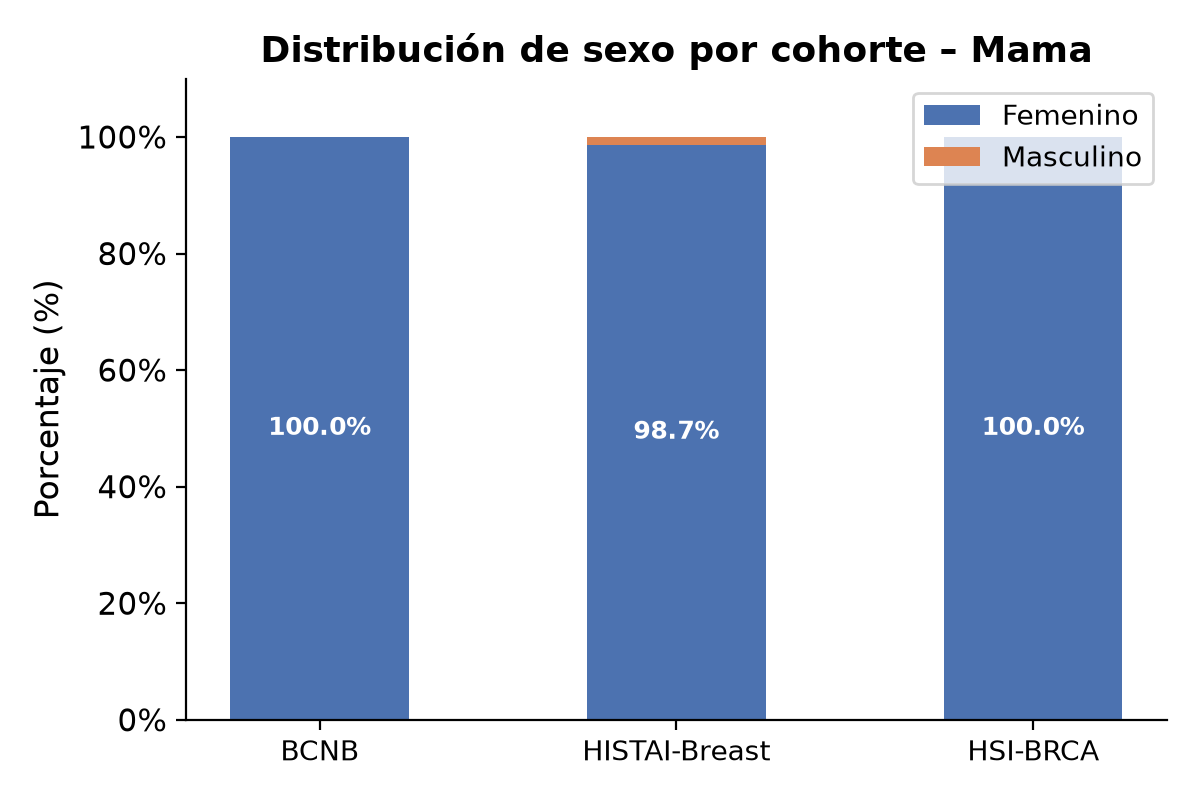
\includegraphics[width=0.65\textwidth]{images/fig_sexo_mama.png}
\caption{Distribución por sexo en los conjuntos de datos de cáncer de mama.}
\label{fig:sexo_mama}
\end{figure}

\begin{figure}[htbp]
\centering
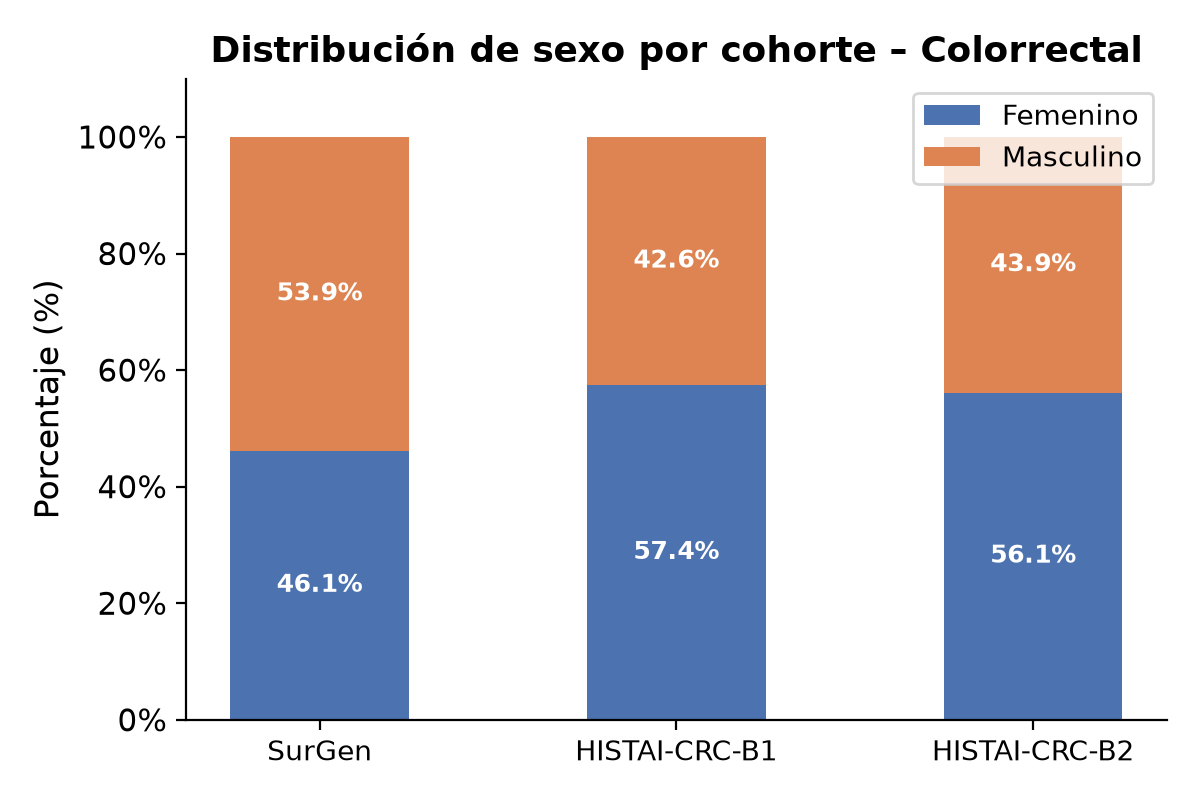
\includegraphics[width=0.65\textwidth]{images/fig_sexo_colorrectal.png}
\caption{Distribución por sexo en los conjuntos de datos de cáncer colorrectal.}
\label{fig:sexo_colorrectal}
\end{figure}

\begin{figure}[htbp]
\centering
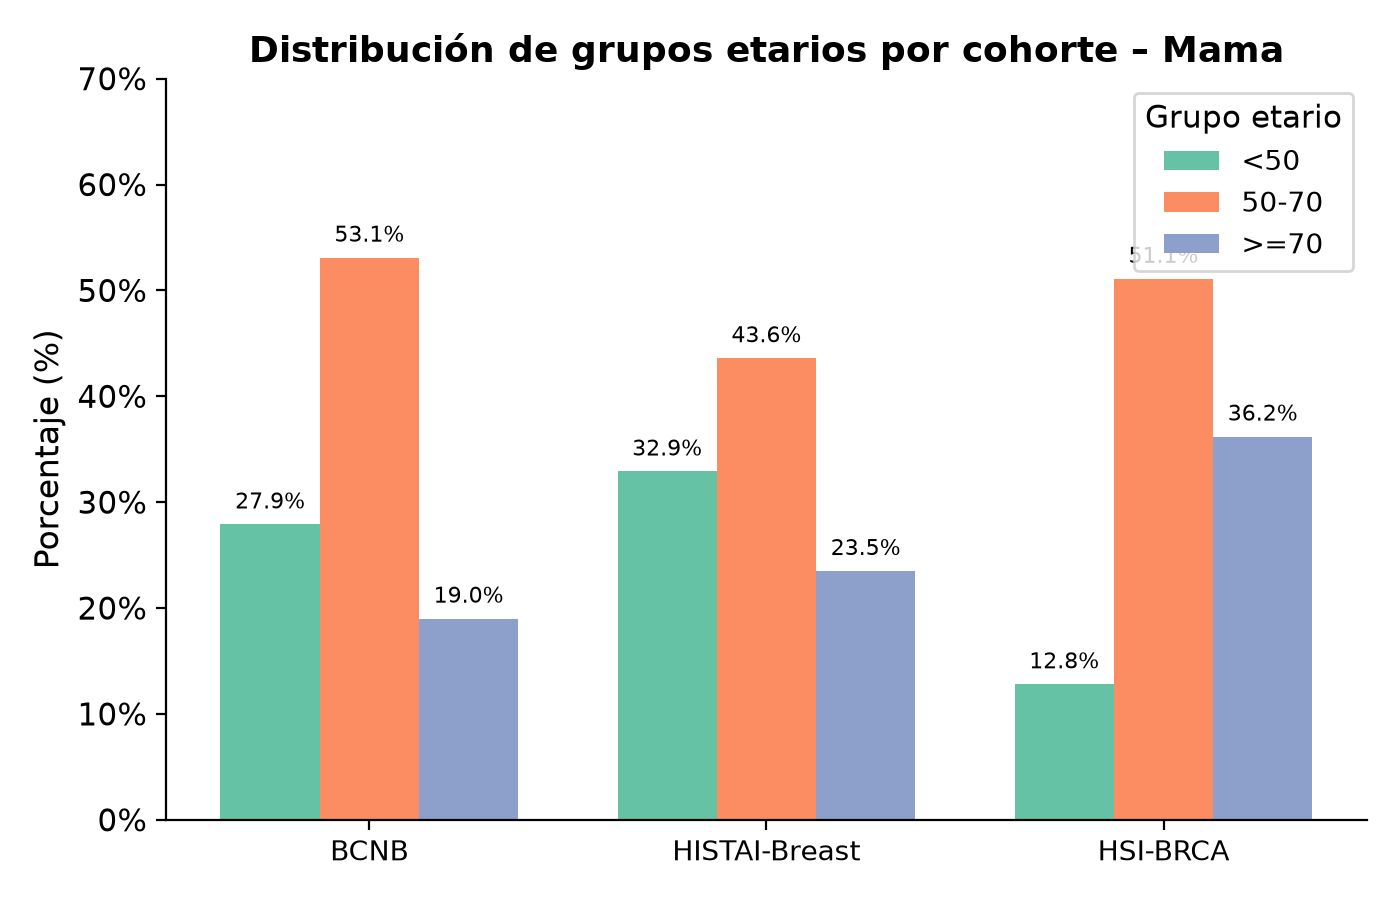
\includegraphics[width=0.65\textwidth]{images/fig_edad_mama.png}
\caption{Distribución por grupos etarios en los conjuntos de datos de cáncer de mama.}
\label{fig:edad_mama}
\end{figure}

\begin{figure}[htbp]
\centering
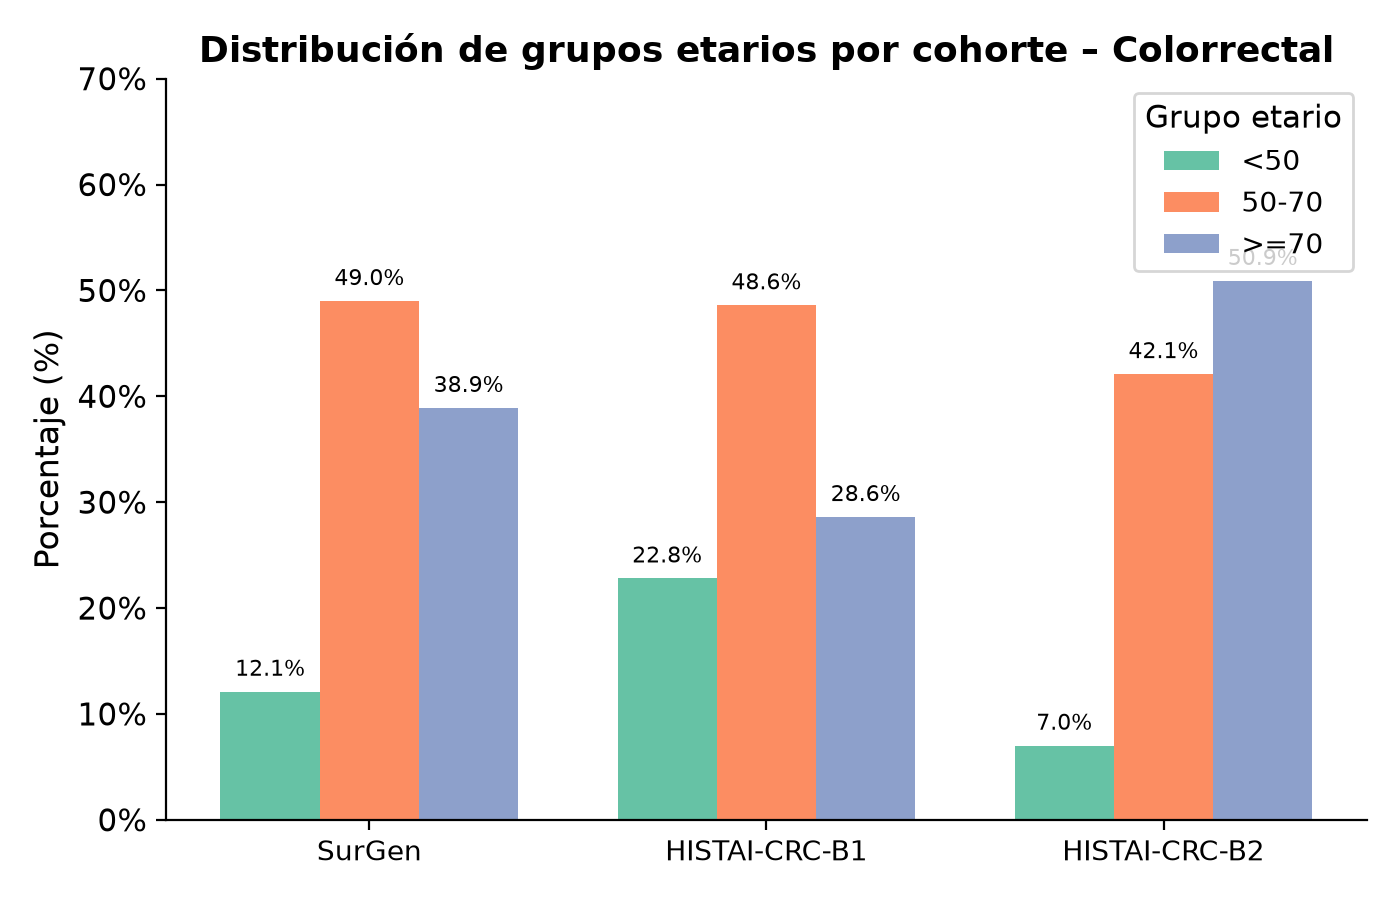
\includegraphics[width=0.65\textwidth]{images/fig_edad_colorrectal.png}
\caption{Distribución por grupos etarios en los conjuntos de datos de cáncer colorrectal.}
\label{fig:edad_colorrectal}
\end{figure}

En mama, las tres cohortes muestran un patrón consistente: distribuciones etarias desplazadas hacia la adultez mayor (medianas entre 57 y 65 años) y una proporción creciente de pacientes de 70 años o más a medida que disminuye el tamaño de la cohorte (19--36\%, Figura~\ref{fig:edad_mama}), lo que constituye una fuente potencial de \textit{bias} de representación. En colorrectal, SurGen e HISTAI-CRC-B2 concentran una proporción considerable de pacientes mayores de 70 años (39\% y 51\%, Figura~\ref{fig:edad_colorrectal}), mientras HISTAI-CRC-B1 es más joven (mediana 63 años); esta heterogeneidad es relevante porque la edad podría correlacionarse con el sitio anatómico y el estado mutacional, introduciendo confusión en análisis comparativos.

\subsection{Distribución de variables objetivo en el dominio de mama}

Se consideraron dos variables objetivo: HER2 (tres clases) y subtipo molecular (cuatro clases), disponibles en las tres cohortes con diferencias de cobertura y forma de reporte (Tabla~\ref{tab:resumen_frecuencias_mama}; cobertura por cohorte en la Tabla~\ref{tab:trazabilidad_mama}).

\subsubsection*{HER2}

La distribución difiere marcadamente entre cohortes: BCNB concentra sus casos entre negativo/bajo y equívoco con baja proporción de positivos; HISTAI-Breast muestra un patrón similar pero con una fracción considerable sin dato recuperable desde texto libre; y HSI-BC presenta fuerte predominio de la categoría negativa, sin equívocos registrados. Estas diferencias podrían reflejar tanto variación real en prevalencia como diferencias en criterios de reporte. En HISTAI-Breast existe además una representación masculina marginal (1,3\%) que, junto con la ausencia total de varianza en sexo en BCNB y HSI-BC, impide el análisis estratificado por sexo en este dominio.

\subsubsection*{Subtipo molecular}

BCNB reporta subtipo para la totalidad de los casos, con predominio de Luminal B y Luminal A. HISTAI-Breast, extraído desde texto libre con 57,2\% de cobertura, muestra un patrón similar pero más concentrado en Luminal B y HER2+. HSI-BC (n=47) presenta predominio de Luminal B con baja representación de HER2+ y Triple negativo, por lo que sus estimaciones deben interpretarse con cautela. En consecuencia, la edad queda como único atributo demográfico utilizable para estratificar comparaciones de \textit{bias} en mama.

\subsection{Distribución de variables objetivo en el dominio colorrectal}

Se consideraron el sitio anatómico del tumor y la lateralidad, armonizados en la curación (Sección~\ref{sec:caracterizacion_datasets}) y reportados en la Tabla~\ref{tab:resumen_frecuencias_colorrectal} (desglose completo en la Tabla~\ref{tab:frecuencias_colorrectal} del Apéndice~\ref{appendix:tablasdatasets}).

\subsubsection*{Sitio anatómico}

Recto, sigmoide y colon derecho concentran la mayoría de los casos en las tres cohortes, con diferencias en la granularidad reportada. Las categorías de baja frecuencia relevantes para \textit{fairness}, rectosigmoide en SurGen (2,3\%) y metástasis hepática en HISTAI-CRC-B1 (2,1\%), concentran pocos casos, implicando mayor variabilidad en esos subgrupos; en HISTAI-CRC-B2 (n=57), cualquier desagregación por sitio debe interpretarse con cautela.

\subsubsection*{Lateralidad}

Definida como simplificación del sitio anatómico (izquierdo, derecho, recto, transverso, rectosigmoide), presenta cobertura parcial (75,0\% en SurGen, 70,0\% en HISTAI-CRC-B1, 80,7\% en HISTAI-CRC-B2). Predominan izquierdo, derecho y recto, mientras transverso y rectosigmoide concentran sistemáticamente menos casos; la lateralidad muestra en general menos desbalance que el sitio anatómico, pero estas categorías de baja frecuencia deben considerarse especialmente en las cohortes más pequeñas.

\subsection{Trazabilidad de muestras a lo largo del pipeline}
\label{sec:trazabilidad_muestras}

Las secciones anteriores describieron las distribuciones demográficas y de variables objetivo sobre la cohorte curada (\textit{post-curation}). Sin embargo, la población efectivamente disponible para una tarea de clasificación puede ser menor, debido a filtros sucesivos: disponibilidad de etiqueta objetivo y completitud de atributos de estratificación (edad, sexo).

Las Tablas~\ref{tab:trazabilidad_mama}~y~\ref{tab:trazabilidad_colorrectal} documentan esta transición para los dominios de mama y colorrectal, respectivamente. Se reportan tres hitos: el tamaño bruto del recurso original (N\textsubscript{raw}), el tamaño después de la curación y armonización (N\textsubscript{curation}), y, para cada variable objetivo, el número de casos de la cohorte analítica final (N\textsubscript{elegible}) y el porcentaje de retención respecto a la cohorte curada. Estos tamaños corresponden exactamente a las poblaciones utilizadas en los experimentos del Capítulo~\ref{cap:evaluacion_modelos}.

\begin{table}[htbp]
\centering
\caption{Trazabilidad de muestras en el dominio de mama.}
\label{tab:trazabilidad_mama}
\footnotesize
\setlength{\tabcolsep}{4pt}
\begin{tabular}{lcccccc}
\toprule
\multirow{2}{*}{\textbf{Dataset}} & \multirow{2}{*}{\textbf{N\textsubscript{raw}}} & \multirow{2}{*}{\textbf{N\textsubscript{cur}}}
  & \multicolumn{2}{c}{\textbf{HER2}} & \multicolumn{2}{c}{\textbf{Subtipo mol.}} \\
\cmidrule(lr){4-5} \cmidrule(lr){6-7}
& & & \textbf{N\textsubscript{ele}} & \textbf{\% ret.} & \textbf{N\textsubscript{ele}} & \textbf{\% ret.} \\
\midrule
BCNB & 1058 & 1058 & 1058 & 100,0 & 1058 & 100,0 \\
HISTAI-Breast & 1489 & 1489 & 870 & 58,4 & 842 & 56,5 \\
HSI-BC & 47 & 47 & 44 & 93,6 & 44 & 93,6 \\
\bottomrule
\end{tabular}
\end{table}

\begin{table}[htbp]
\centering
\caption{Trazabilidad de muestras en el dominio colorrectal.}
\label{tab:trazabilidad_colorrectal}
\footnotesize
\setlength{\tabcolsep}{4pt}
\begin{tabular}{lcccccc}
\toprule
\multirow{2}{*}{\textbf{Dataset}} & \multirow{2}{*}{\textbf{N\textsubscript{raw}}} & \multirow{2}{*}{\textbf{N\textsubscript{cur}}}
  & \multicolumn{2}{c}{\textbf{Sitio}} & \multicolumn{2}{c}{\textbf{Lateralidad}} \\
\cmidrule(lr){4-5} \cmidrule(lr){6-7}
& & & \textbf{N\textsubscript{ele}} & \textbf{\% ret.} & \textbf{N\textsubscript{ele}} & \textbf{\% ret.} \\
\midrule
SurGen & 843 & 841 & 765 & 91,0 & 631 & 75,0 \\
HISTAI-CRC-B1 & 878 & 878 & 878 & 100,0 & 615 & 70,0 \\
HISTAI-CRC-B2 & 57 & 57 & 57 & 100,0 & 46 & 80,7 \\
\bottomrule
\end{tabular}
\end{table}

Como se observa en las tablas, HISTAI-Breast presenta la mayor pérdida de casos en mama (56--58\% de retención), debido a la naturaleza no estructurada de los informes desde los que se extrajeron los biomarcadores. En colorrectal, la lateralidad tiene sistemáticamente menor cobertura que el sitio anatómico, reflejando que no todos los casos con sitio clasificable admiten una lateralidad definida (por ejemplo, sitios inespecíficos o metastásicos). La descripción de las reglas de extracción empleadas, sus criterios de resolución de conflictos y sus errores esperables se presenta en el Apéndice~\ref{appendix:extraccion_histai}.

Esta pérdida puede además alterar la composición demográfica de la población analizable: en HISTAI-Breast, la mediana de edad se desplaza de 58 a 63 años al filtrar por HER2 o subtipo molecular, con menos casos menores de 50 años y más mayores de 70, lo que sugiere que los pacientes mayores tienen mayor probabilidad de contar con biomarcadores extraíbles, un sesgo de selección indirecto por edad en la cohorte elegible.

\subsection{Condiciones de adquisición y potencial de confusión}
\label{sec:adquisicion}

La Tabla~\ref{tab:adquisicion_bias} resume los parámetros de adquisición documentados para cada conjunto de datos seleccionado. Como puede observarse, existe una asociación casi perfecta entre dataset y condiciones de adquisición: todos los casos de un mismo recurso fueron digitalizados con el mismo escáner (o un conjunto acotado de ellos), bajo la misma magnificación y tinción. Esto implica que, en cualquier comparación entre cohortes, la variable \textit{dataset} puede estar confundida con el equipo de digitalización, el protocolo de tinción y el período de recolección.

\begin{table}[htbp]
\centering
\caption{Parámetros de adquisición y riesgo de confusión entre cohortes.}
\label{tab:adquisicion_bias}
\small
\setlength{\tabcolsep}{4pt}
\resizebox{\textwidth}{!}{%
\begin{tabular}{lllll}
\toprule
\textbf{Dataset} & \textbf{Escáner} & \textbf{Magnif.} & \textbf{Tinción} & \textbf{Período} \\
\midrule
BCNB & No reportado & 20x & H\&E & No reportado \\
HISTAI-Breast & Leica Aperio GT450/AT2 & 20x (40x frac.) & H\&E (mayoría) & No reportado \\
HSI-BC & 3DHISTECH P250 Flash III & 20x & H\&E + hiperesp. & 2006--2015 \\
SurGen & ZEISS AxioScan.Z1 & 40x & H\&E & No reportado \\
HISTAI-CRC-B1 & Leica Aperio GT450/AT2 & 20x (40x frac.) & H\&E (mayoría) & No reportado \\
HISTAI-CRC-B2 & Leica Aperio GT450/AT2 & 20x (40x frac.) & H\&E (mayoría) & No reportado \\
\bottomrule
\end{tabular}%
}
\end{table}

Esta confusión tiene implicancias directas para comparaciones \textit{cross-dataset}: una diferencia de desempeño entre BCNB e HISTAI-Breast no podrá atribuirse solo a edad o subtipo molecular, ya que ambas cohortes difieren en escáner, institución y método de determinación de biomarcadores (estructurado vs. extraído de texto libre, con la pérdida selectiva documentada en la Sección~\ref{sec:trazabilidad_muestras}). En colorrectal, aunque las tres cohortes comparten tinción H\&E, persiste diferencia de escáner y magnificación (40x en SurGen vs. 20x en HISTAI); por ello se utilizará la versión a 20x de SurGen, unificando la resolución de trabajo. Esta confusión entre \textit{dataset} y condiciones técnicas corresponde a la principal fuente de sobreestimación de desempeño identificada en patología computacional: cuando \textit{dataset} y centro de origen coinciden, un modelo puede explotar la firma técnica del centro en lugar de la morfología de interés, ventaja que no se transfiere a cohortes externas \parencite{howard2021site}. Este estudio documenta la condición a nivel de metadatos; su efecto sobre el desempeño y las brechas entre subgrupos se evalúa experimentalmente en los Capítulos~\ref{cap:seleccion_modelos}~y~\ref{cap:evaluacion_modelos}.

\subsection{Síntesis de indicadores de \textit{bias} por conjunto de datos}
\label{sec:sintesis_bias}

A modo de síntesis, la Tabla~\ref{tab:matriz_riesgo_unificada} presenta una visión consolidada de los indicadores de \textit{bias} identificados para cada conjunto de datos seleccionado, organizados según los tres mecanismos definidos en la Sección~\ref{sec:marco_bias}: representación, adquisición y documentación/selección. Para cada mecanismo se asigna un nivel de riesgo cualitativo (bajo, medio, alto) basado en la evidencia presentada a lo largo del capítulo, junto con una columna de riesgo global que integra los tres ejes. Los criterios de asignación de cada nivel se detallan en el Apéndice~\ref{appendix:criterios_preseleccion}.

\begin{table}[htbp]
\centering
\caption{Matriz unificada de riesgo de \textit{bias} por conjunto de datos seleccionado.}
\label{tab:matriz_riesgo_unificada}
\small
\setlength{\tabcolsep}{5pt}
\begin{tabular}{lcccc}
\toprule
\textbf{Dataset} &
  \textbf{Representación} &
  \textbf{Adquisición} &
  \textbf{Documentación} &
  \textbf{Riesgo global} \\
\midrule
BCNB &
  \cellcolor{riesgobajo}Bajo &
  \cellcolor{riesgomedio}Medio &
  \cellcolor{riesgobajo}Bajo &
  \cellcolor{riesgobajo}Bajo--Medio \\
HISTAI-Breast &
  \cellcolor{riesgomedio}Medio &
  \cellcolor{riesgomedio}Medio &
  \cellcolor{riesgoalto}Alto &
  \cellcolor{riesgomedio}Medio--Alto \\
HSI-BC &
  \cellcolor{riesgoalto}Alto &
  \cellcolor{riesgobajo}Bajo &
  \cellcolor{riesgobajo}Bajo &
  \cellcolor{riesgoalto}Alto \\
SurGen &
  \cellcolor{riesgobajo}Bajo--Medio &
  \cellcolor{riesgomedio}Medio &
  \cellcolor{riesgomedio}Medio &
  \cellcolor{riesgomedio}Medio \\
HISTAI-CRC-B1 &
  \cellcolor{riesgomedio}Medio &
  \cellcolor{riesgomedio}Medio &
  \cellcolor{riesgomedio}Medio &
  \cellcolor{riesgomedio}Medio \\
HISTAI-CRC-B2 &
  \cellcolor{riesgoalto}Alto &
  \cellcolor{riesgomedio}Medio &
  \cellcolor{riesgobajo}Bajo &
  \cellcolor{riesgoalto}Alto \\
\bottomrule
\end{tabular}
\end{table}

Esto permite identificar patrones transversales: los riesgos más altos se concentran en cohortes de tamaño muy reducido (HSI-BC, HISTAI-CRC-B2), donde la capacidad de realizar análisis estratificados es limitada y cualquier estimación por subgrupo presentará intervalos de confianza amplios. En el extremo opuesto, BCNB destaca como el conjunto de datos con perfil de riesgo más bajo, debido a su tamaño adecuado, completitud casi perfecta y disponibilidad de múltiples variables clínicas estructuradas. HISTAI-Breast presenta un perfil mixto: si bien su tamaño es moderado, el sesgo de selección inducido por la extracción desde texto libre eleva su riesgo de documentación a niveles que deben considerarse al interpretar cualquier análisis basado en esta cohorte.

En cuanto a los mecanismos de \textit{bias}, el de adquisición es el más uniforme entre cohortes: prácticamente todos los conjuntos presentan confusión entre dataset y condiciones técnicas, lo que obliga a considerar este factor en cualquier comparación \textit{cross-dataset}. El \textit{bias} de representación, en cambio, es más variable y depende del dominio: en mama está acotado principalmente a la edad, mientras que en colorrectal permite análisis más ricos al contar con variabilidad en sexo y edad simultáneamente.

\subsection{Implicancias para el análisis de \textit{bias} en etapas posteriores}
\label{sec:implicancias_bias}

El análisis cuantitativo realizado permite extraer varias conclusiones relevantes para la formulación de tareas y la interpretación de resultados en los capítulos siguientes.

En primer lugar, la variable sexo no puede utilizarse como atributo sensible en el dominio de mama, dado que las tres cohortes son abrumadoramente femeninas. Esto no elimina la posibilidad de que existan sesgos de representación por sexo, especialmente si los modelos entrenados exclusivamente con datos femeninos se aplican a pacientes masculinos, pero sí significa que no es posible construir grupos de comparación intra-dataset. En colorrectal, en cambio, el sexo presenta una distribución suficientemente equilibrada como para permitir análisis estratificados, aunque algunas combinaciones de sitio anatómico y sexo presentan tamaños muestrales reducidos.

En segundo lugar, la edad emerge como la variable demográfica más prometedora para el análisis estratificado, al estar disponible con completitud total dentro de la cohorte curada en los seis conjuntos de datos y presentar una distribución con varianza suficiente en todos ellos. Sin embargo, las diferencias en la distribución etaria entre cohortes de un mismo dominio deben ser consideradas al interpretar comparaciones entre conjuntos de datos, ya que podrían reflejar diferencias reales en la población de origen o sesgos de selección en los criterios de inclusión de cada estudio.

En tercer lugar, el análisis de las variables objetivo en cada dominio reveló que ciertas categorías presentan una prevalencia muy baja. Esta condición implica que cualquier análisis estratificado sobre dichos subgrupos producirá estimaciones con intervalos de confianza más amplios y, por lo tanto, con menor capacidad para distinguir una brecha real de una fluctuación muestral. Esta limitación es reconocida en la literatura de \textit{fairness} en imagen médica, donde la escasa representación de determinados subgrupos restringe tanto la fiabilidad de las métricas desagregadas como la aplicabilidad de las técnicas de evaluación de equidad, que en su mayoría requieren subgrupos de tamaño suficiente \parencite{riccilara2022fairness,wastvedt2024small}. El manejo experimental de estas categorías se retoma en el Capítulo~\ref{cap:seleccion_modelos}.

La heterogeneidad observada no invalida el uso de estos conjuntos de datos, sino que define los límites dentro de los cuales pueden realizarse inferencias válidas, límites que se retoman en la formulación experimental de los Capítulos~\ref{cap:seleccion_modelos}~y~\ref{cap:evaluacion_modelos}.

El análisis de sesgo racial/étnico se declara fuera de alcance (ver §\ref{sec:conclusiones_capitulo4}).

\section{Conclusiones del capítulo}
\label{sec:conclusiones_capitulo4}

Este capítulo cumplió el objetivo específico~1 de la tesis: caracterizar los conjuntos de datos disponibles para el estudio de \textit{bias} en patología digital, identificando condiciones de representación, calidad de metadatos y limitaciones de comparabilidad entre cohortes. Los hallazgos obtenidos permiten establecer una base empírica sobre la cual formular tareas de clasificación y diseñar experimentos de evaluación de \textit{fairness} en los capítulos siguientes.

La revisión de nueve recursos públicos iniciales permitió constatar la heterogeneidad estructural que caracteriza al panorama actual de conjuntos de datos de patología digital. Esta heterogeneidad se manifestó en múltiples dimensiones: tamaño de las cohortes (desde 47 hasta más de mil registros), nivel de estructuración de los metadatos, completitud de variables clínicas y parámetros de adquisición. Tras aplicar un proceso sistemático de curación y armonización, se priorizaron seis conjuntos de datos en dos dominios clínicos, mama y colorrectal, seleccionados por presentar variables comparables entre cohortes y viabilidad para formular tareas supervisadas con al menos dos conjuntos por dominio.

La aplicación del marco de \textit{bias} basado en tres mecanismos (representación, adquisición y documentación/selección) reveló que todos los conjuntos de datos presentan algún grado de riesgo potencial, aunque de distinta naturaleza e intensidad. En el dominio de mama, la principal limitación para el análisis de \textit{fairness} es la variabilidad insuficiente de la variable sexo: BCNB y HSI-BC son exclusivamente femeninos, e HISTAI-Breast contiene una fracción masculina marginal (n=20; 1,3\%), insuficiente para un análisis estratificado estable, lo que restringe los atributos sensibles disponibles exclusivamente a la edad. Este hallazgo es consistente con la literatura sobre cáncer de mama, donde la incidencia masculina es sustancialmente menor, y obliga a considerar la edad como el único eje de estratificación demográfica en este dominio. En el dominio colorrectal, en cambio, tanto sexo como edad presentan distribuciones con varianza suficiente, lo que habilita análisis estratificados más ricos.

En cuanto al eje racial/étnico, dos de los recursos revisados (HSI-BC y NDB-UFES) registran información de raza y etnia, pero ninguna de estas cohortes es susceptible de estratificación: NDB-UFES fue excluida en la preselección y HSI-BC (n=47) no proporciona potencia estadística para desagregar. El resto de las cohortes no contienen esta variable, por lo que el sesgo racial/étnico queda fuera de alcance en este diagnóstico.

La trazabilidad de las muestras a lo largo del \textit{pipeline} de datos evidenció que el proceso de extracción de etiquetas no es neutro: en HISTAI-Breast, la necesidad de recuperar biomarcadores desde texto libre introdujo un sesgo de selección etario, desplazando la mediana de edad de 58 a 63 años. Este resultado constituye una advertencia metodológica importante, ya que sugiere que la calidad de la documentación de un conjunto de datos no solo afecta la cantidad de casos utilizables, sino también la composición demográfica de la cohorte analítica. Trabajos recientes han señalado que este tipo de sesgos de documentación suele estar infrarreportado en la literatura de patología computacional \parencite{galanty2024}, lo que refuerza la necesidad de hacerlos explícitos. La metodología de dicha extracción y sus límites de validación se detallan en el Apéndice~\ref{appendix:extraccion_histai}.

En términos de condiciones de adquisición, se documentó una asociación casi perfecta entre conjunto de datos y parámetros técnicos (escáner, magnificación, tinción), lo que implica que cualquier comparación entre cohortes confunde necesariamente diferencias poblacionales con diferencias técnicas. Esta confusión conecta con dos hallazgos distintos de la literatura, que conviene diferenciar. Por una parte, se ha demostrado que el sitio de adquisición puede ser \textbf{inferido} a partir de imágenes histopatológicas digitalizadas, lo que evidencia la existencia de una firma institucional detectable en la propia imagen \parencite{alsaafin2023biased}. Por otra parte, se ha documentado que dichas firmas específicas de sitio \textbf{afectan el desempeño de los modelos}: persisten pese a la normalización de tinción y a las estrategias habituales de aumentación de datos, inducen estimaciones sesgadas de exactitud cuando muestras de un mismo centro aparecen simultáneamente en entrenamiento y validación, y permiten incluso inferir atributos demográficos como la etnia a partir de la procedencia institucional \parencite{howard2021site}. Este segundo fenómeno es el que la literatura denomina \textit{center effect} o \textit{batch effect} propiamente tal.

La distinción es relevante para esta tesis: el presente capítulo documenta únicamente la condición estructural que hace posible ambos fenómenos, la asociación entre cohorte y parámetros técnicos (Sección~\ref{sec:adquisicion}), pero no demuestra que dicha confusión se traduzca efectivamente en un sesgo de desempeño en los modelos evaluados. La existencia de esta confusión no invalida las comparaciones entre cohortes, pero exige interpretar con cautela cualquier diferencia de desempeño \textit{cross-dataset}. La verificación empírica de este riesgo se aborda en el Capítulo~\ref{cap:evaluacion_modelos}, donde se evalúa experimentalmente la magnitud del \textit{center effect} en las comparaciones entre conjuntos de datos.

Los resultados de esta caracterización tienen implicancias directas para el diseño experimental de los capítulos siguientes. En primer lugar, las tareas de clasificación deberán definirse considerando la cobertura real de etiquetas por cohorte, particularmente en HISTAI-Breast donde la extracción desde texto libre limitó la disponibilidad de biomarcadores. En segundo lugar, la comparabilidad semántica de las categorías entre cohortes deberá verificarse explícitamente, especialmente en lo relativo a HER2, donde los criterios de reporte difieren entre conjuntos de datos. En tercer lugar, la evaluación de \textit{fairness} se centrará en la edad como atributo sensible en mama, y en edad y sexo en colorrectal, con la advertencia de que los subgrupos con menor representación muestral producirán estimaciones con intervalos de confianza más amplios, lo que limita la potencia del análisis desagregado \parencite{riccilara2022fairness}.

Lo que este capítulo no permite concluir es igualmente relevante: los indicadores observables aquí identificados no constituyen una prueba de que los modelos entrenados con estos datos exhibirán disparidades de rendimiento. La traducción de estos indicadores en \textit{bias} efectivo depende de la interacción entre las distribuciones de los datos, la arquitectura del modelo y el algoritmo de optimización. Esta distinción entre \textit{bias} potencial en los datos y \textit{bias} efectivo en los modelos es central en la literatura de \textit{fairness} en inteligencia artificial \parencite{mehrabi2021survey}, y será retomada en el Capítulo~\ref{cap:evaluacion_modelos} al contrastar los resultados experimentales con las condiciones de representación documentadas en esta caracterización.

	\chapter{Selección de Modelos Fundacionales y Definición de Tareas}
\label{cap:seleccion_modelos}

El Capítulo \ref{cap:caracterizacion_datasets} presentó la caracterización, preselección y armonización de los conjuntos de datos considerados en este estudio. A partir de dicho proceso, se priorizaron los dominios de cáncer de mama y cáncer colorrectal, debido a la disponibilidad de más de una cohorte por dominio y a la posibilidad de construir espacios de comparación mediante variables clínicas, demográficas y anatómicas armonizadas.

De esta forma, el presente capítulo aborda la selección de modelos fundacionales representativos para las tareas definidas en el ámbito del análisis de \textit{Whole Slide Images} de patología digital, de acuerdo con las características de los conjuntos de datos analizados. La selección no busca identificar un modelo universalmente superior, sino construir un conjunto de modelos que permita realizar una comparación experimental controlada de sus representaciones y de su comportamiento frente a variaciones entre cohortes y subgrupos. Este capítulo se limita a la selección de modelos y la definición de las tareas de evaluación.

Los modelos fundacionales en patología digital han demostrado que el preentrenamiento auto-supervisado a gran escala permite obtener representaciones visuales transferibles a múltiples tareas posteriores. Sin embargo, las diferencias entre los datos de preentrenamiento, las arquitecturas utilizadas, las estrategias de aprendizaje y el grado de documentación disponible pueden afectar tanto la reproducibilidad de los experimentos como la interpretación de sus resultados.

\section{Criterios de selección}
\label{sec:criterios_seleccion}

\begin{table}[htbp]
\centering
\caption{Criterios empleados para la selección de modelos fundacionales.}
\label{tab:criterios_seleccion_modelos}
\small
\renewcommand{\arraystretch}{1.12}
\begin{tabular}{p{3.7cm} p{10.3cm}}
\toprule
\textbf{Criterio} & \textbf{Descripción y relevancia para el estudio} \\
\midrule

Pertinencia de dominio &
Se priorizaron modelos preentrenados para patología computacional o con uso predominante de imágenes histopatológicas. Esto permite mantener coherencia entre el dominio de preentrenamiento y las WSI de patología digital empleadas en el estudio. \\

Compatibilidad con WSI H\&E &
Se consideró la capacidad de procesar parches provenientes de WSI teñidas principalmente con hematoxilina y eosina (H\&E), modalidad predominante en las cohortes seleccionadas. Además, los modelos debían poder utilizarse como extractores de representaciones bajo un protocolo experimental común. \\

Accesibilidad y reproducibilidad &
Se requirió acceso público a pesos preentrenados e implementación documentada, mediante repositorios oficiales, código de referencia o interfaces de uso. Esto permite reproducir los experimentos sin reentrenar los modelos desde cero y reduce ambigüedades de implementación. \\

Documentación técnica &
Se evaluó la disponibilidad de artículos, \textit{model cards} o documentación oficial que describiera la arquitectura, los requisitos de entrada, el preprocesamiento y la estrategia de preentrenamiento. Esta información permite utilizar los modelos de manera consistente e interpretar sus resultados. \\

Trazabilidad del preentrenamiento &
Se revisó la información pública sobre procedencia, modalidad y escala de los datos de preentrenamiento, incluyendo posibles solapamientos con las cohortes de evaluación. Las limitaciones de documentación se registran explícitamente, debido a su relevancia para interpretar generalización y sesgo. \\

Diversidad metodológica controlada &
Se buscaron diferencias en arquitectura, estrategia de aprendizaje, escala o procedencia de los datos de preentrenamiento. Sin embargo, se exigió compatibilidad con una comparación homogénea basada en embeddings, evitando que componentes adicionales del \textit{pipeline} condicionen los resultados. \\

Viabilidad computacional &
Se evaluó la factibilidad de ejecutar la inferencia en la infraestructura disponible, considerando memoria GPU, tiempo de procesamiento y almacenamiento. Se priorizó el uso de los modelos como extractores de representaciones, sin realizar reentrenamiento completo. \\

\bottomrule
\end{tabular}
\end{table}

Los criterios se orientan a equilibrar la representatividad de los modelos con la reproducibilidad del estudio. En particular, la disponibilidad de código y pesos constituye una condición práctica necesaria para construir un protocolo de evaluación homogéneo. Por otra parte, la trazabilidad de los datos de preentrenamiento es especialmente relevante en un estudio de \textit{bias} y \textit{fairness}, ya que un posible solapamiento entre los datos usados para preentrenar un modelo y las cohortes de evaluación podría sobreestimar su capacidad de generalización.

\section{Modelos seleccionados}
\label{sec:modelos_seleccionados}

Como resultado del proceso descrito, se seleccionaron los modelos Phikon-v2 \parencite{filiot2024phikonv2}, UNI2 \parencite{chen2024uni}, Prov-GigaPath \parencite{xu2024provgigapath} y Virchow2 \parencite{vorontsov2024virchow}. Los cuatro modelos fueron diseñados para el dominio de patología computacional y disponen de mecanismos de acceso documentados a sus pesos e implementación, ya sea abierto o mediante registro y aceptación de términos. Esto permite utilizarlos como extractores de representaciones visuales dentro de un protocolo experimental común.

La selección busca mantener un equilibrio entre diversidad metodológica y factibilidad experimental. Los modelos seleccionados difieren en la escala y composición reportada de sus datos de preentrenamiento, en sus arquitecturas base y en sus estrategias de aprendizaje auto-supervisado. Sin embargo, comparten una característica central para este estudio: pueden utilizarse como extractores de representaciones visuales para parches provenientes de WSI.

La comparación experimental se realizará manteniendo constante el protocolo posterior al \textit{encoder}. Para cada tarea se utilizarán procedimientos equivalentes de preparación de datos, extracción de embeddings, agregación a nivel de WSI y entrenamiento del clasificador final. De esta manera, las diferencias observadas en utilidad predictiva, estabilidad entre cohortes y disparidades entre subgrupos podrán atribuirse con mayor claridad a las representaciones generadas por cada modelo.

La Tabla~\ref{tab:atributos_modelos}, presentada en el Anexo~\ref{apx:atributos_modelos}, resume los atributos técnicos y de trazabilidad de cada modelo. La disponibilidad desigual de información sobre los datos de preentrenamiento se registrará explícitamente como limitación, particularmente ante la posibilidad de solapamiento entre dichos datos y las cohortes de evaluación. Esta limitación no invalida el análisis, pero restringe la atribución causal de las diferencias de rendimiento y debe considerarse al discutir los resultados obtenidos.

Con el fin de complementar la Tabla~\ref{tab:atributos_modelos} (Anexo~\ref{apx:atributos_modelos}),
a continuación se describe brevemente la arquitectura y el
esquema de preentrenamiento de cada modelo seleccionado.

\textbf{Phikon-v2} corresponde a un \textit{Vision Transformer} de tipo ViT-L/16
(aproximadamente 0.3 mil millones de parámetros), preentrenado mediante la receta
auto-supervisada DINOv2 sobre el corpus público PANCAN-XL, compuesto por 456
millones de parches de $224\times224$ píxeles a 20x de magnificación, extraídos de
más de 58.000 WSI provenientes de TCGA, CPTAC y GTEx \citep{filiot2024phikonv2}.
El token \texttt{[CLS]} resultante entrega un embedding de 1024 dimensiones por parche.

\textbf{UNI2-h} utiliza una variante personalizada ViT-H/14 (681 millones de
parámetros), entrenada con la receta DINOv2 sobre más de 200 millones de parches
H\&E e IHC muestreados de 350.000 WSI institucionales de Mass General Brigham
\citep{chen2024uni}. Entrega un embedding de 1536 dimensiones.

\textbf{Prov-GigaPath} adopta una arquitectura jerárquica de dos etapas: un
encoder de parche ViT-g/14 preentrenado con DINOv2 sobre 1.300 millones de
parches de $256\times256$ píxeles provenientes de 171.189 WSI H\&E e IHC del
sistema de salud Providence, seguido de un encoder de \textit{slide} basado en
LongNet, un transformer con atención dilatada de complejidad lineal, entrenado
mediante un autoencoder enmascarado \citep{xu2024provgigapath}. En esta tesis se
utiliza únicamente el encoder de parche como extractor de representaciones
(1536 dimensiones), sin emplear el agregador de \textit{slide} completo.

\textbf{Virchow2} corresponde a un ViT-H/14 (632 millones de parámetros)
entrenado con una variante multiescala de DINOv2 sobre 3.1 millones de WSI
H\&E y 400.000 WSI IHC que abarcan 40 tipos de tejido, incorporando durante el
preentrenamiento parches muestreados a 5x, 10x, 20x y 40x de magnificación
\citep{vorontsov2024virchow}. Entrega un embedding de 2560 dimensiones por parche, compuesto por la
concatenación del token \texttt{[CLS]} y el promedio de los tokens de parche
de la última capa del transformer.

La Figura~\ref{fig:arquitecturas_modelos} resume de forma esquemática las
cuatro arquitecturas descritas, destacando las diferencias en unidad de
entrada (parche vs.\ parche + slide), mecanismo de agregación de contexto y
dimensión del embedding resultante.

% Borrador de la Figura "fig:arquitecturas_modelos"
% Resume esquemáticamente las cuatro arquitecturas descritas en la Sección 5.2:
% unidad de entrada, encoder/estrategia de preentrenamiento, mecanismo de
% agregación de contexto y dimensión del embedding resultante.
%
% Requiere en el preámbulo del documento:
% \usepackage{tikz}
% \usetikzlibrary{shapes.geometric, arrows.meta, positioning, fit}

\begin{figure}[htbp]
\centering
\resizebox{\textwidth}{!}{%
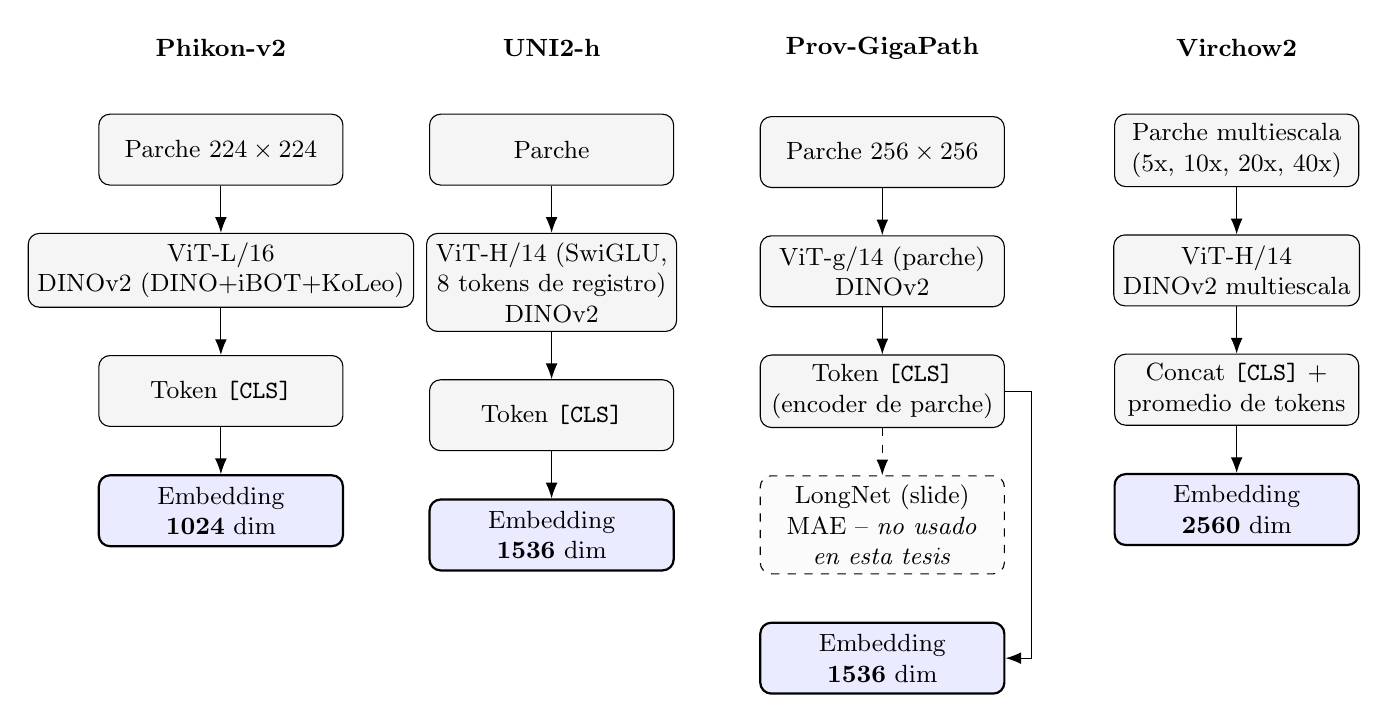
\begin{tikzpicture}[
  font=\small,
  node distance=6mm,
  box/.style={draw, rounded corners, minimum width=3.1cm, minimum height=0.9cm,
              align=center, fill=gray!8},
  boxdashed/.style={box, dashed, fill=gray!3},
  embed/.style={draw, rounded corners, minimum width=3.1cm, minimum height=0.9cm,
                align=center, fill=blue!8, thick},
  title/.style={font=\small\bfseries},
  arr/.style={-{Latex[length=2mm]}}
]

% ---------- Columna 1: Phikon-v2 ----------
\node[title] (t1) at (0,0) {Phikon-v2};
\node[box, below=of t1] (in1) {Parche $224\times224$};
\node[box, below=of in1] (enc1) {ViT-L/16\\DINOv2 (DINO+iBOT+KoLeo)};
\node[box, below=of enc1] (agg1) {Token \texttt{[CLS]}};
\node[embed, below=of agg1] (emb1) {Embedding\\\textbf{1024} dim};
\draw[arr] (in1)--(enc1); \draw[arr] (enc1)--(agg1); \draw[arr] (agg1)--(emb1);

% ---------- Columna 2: UNI2-h ----------
\node[title] (t2) at (4.2,0) {UNI2-h};
\node[box, below=of t2] (in2) {Parche};
\node[box, below=of in2] (enc2) {ViT-H/14 (SwiGLU,\\8 tokens de registro)\\DINOv2};
\node[box, below=of enc2] (agg2) {Token \texttt{[CLS]}};
\node[embed, below=of agg2] (emb2) {Embedding\\\textbf{1536} dim};
\draw[arr] (in2)--(enc2); \draw[arr] (enc2)--(agg2); \draw[arr] (agg2)--(emb2);

% ---------- Columna 3: Prov-GigaPath ----------
\node[title] (t3) at (8.4,0) {Prov-GigaPath};
\node[box, below=of t3] (in3) {Parche $256\times256$};
\node[box, below=of in3] (enc3) {ViT-g/14 (parche)\\DINOv2};
\node[box, below=of enc3] (agg3) {Token \texttt{[CLS]}\\(encoder de parche)};
\node[boxdashed, below=of agg3] (slide3) {LongNet (slide)\\MAE -- \emph{no usado}\\\emph{en esta tesis}};
\node[embed, below=of slide3] (emb3) {Embedding\\\textbf{1536} dim};
\draw[arr] (in3)--(enc3); \draw[arr] (enc3)--(agg3);
\draw[arr, dashed] (agg3)--(slide3);
\draw[arr] (agg3) -- ++(1.9,0) |- (emb3.east);

% ---------- Columna 4: Virchow2 ----------
\node[title] (t4) at (12.9,0) {Virchow2};
\node[box, below=of t4] (in4) {Parche multiescala\\(5x, 10x, 20x, 40x)};
\node[box, below=of in4] (enc4) {ViT-H/14\\DINOv2 multiescala};
\node[box, below=of enc4] (agg4) {Concat \texttt{[CLS]} +\\promedio de tokens};
\node[embed, below=of agg4] (emb4) {Embedding\\\textbf{2560} dim};
\draw[arr] (in4)--(enc4); \draw[arr] (enc4)--(agg4); \draw[arr] (agg4)--(emb4);

\end{tikzpicture}
}
\caption{Comparación esquemática de las arquitecturas de los cuatro modelos fundacionales seleccionados, destacando la unidad de entrada, el mecanismo de agregación de contexto y la dimensión del embedding resultante. El bloque punteado en Prov-GigaPath indica el agregador de \textit{slide} basado en LongNet, no utilizado en esta tesis.}
\label{fig:arquitecturas_modelos}
\end{figure}


Los cuatro modelos se utilizaron como extractores de representaciones congelados (\textit{frozen}), sin realizar ajuste fino (\textit{fine-tuning}) de sus pesos durante el entrenamiento de los clasificadores posteriores. Esta decisión, consistente con el protocolo experimental del Capítulo~\ref{cap:evaluacion_modelos}, garantiza que las diferencias observadas en las métricas de evaluación sean atribuibles a las representaciones preentrenadas y no a adaptaciones específicas del clasificador a cada tarea. El registro de versiones de \textit{checkpoints}, repositorios y entorno de ejecución de cada modelo se documenta en el registro de modelos del estudio (Sección~\ref{sec:protocolo-inferencia}, Capítulo~\ref{cap:evaluacion_modelos}).

\section{Definición de tareas de evaluación}
\label{sec:definicion_tareas}

La selección de modelos se complementa con la definición de tareas de evaluación, dado que el valor de una representación fundacional depende de su desempeño en problemas concretos y de su comportamiento frente a variaciones entre cohortes y subgrupos. Las tareas se definieron utilizando las variables armonizadas en el Capítulo \ref{cap:caracterizacion_datasets}, priorizando aquellas que presentan significado clínico, cobertura suficiente y potencial de comparación entre conjuntos de datos.

En el dominio de cáncer de mama, las variables armonizadas incluyeron, entre otras, edad, estado de receptores hormonales, HER2, Ki-67 y subtipo molecular. Esta disponibilidad permite plantear tareas de clasificación basadas en biomarcadores relevantes, en particular la predicción del estado de HER2 y la clasificación del subtipo molecular.

La variable HER2 se define en tres categorías: negativo (HER2 0/1+), equívoco (HER2 2+) y positivo (HER2 3+), de acuerdo con los criterios de reporte de cada cohorte. El subtipo molecular incluye cuatro categorías (Luminal A, Luminal B, HER2+ y Triple negativo), aunque en HISTAI-Breast dicha variable se extrajo desde texto libre no estructurado, lo que introduce incertidumbre en la comparabilidad semántica entre cohortes.

En el dominio de cáncer colorrectal, el espacio común de variables resultó más acotado y se concentró principalmente en edad, sexo, sitio anatómico y lateralidad. Por esta razón, son las escogidas para su análisis. Además, estas variables se encuentran disponibles de manera más consistente entre las cohortes seleccionadas. Cabe notar que la lateralidad se deriva directamente del sitio anatómico, por lo que ambas tareas capturan en gran medida la misma señal morfológica, con distinto nivel de granularidad.

La Tabla \ref{tab:tareas_evaluacion_preliminares} resume las tareas propuestas. Su definición final dependerá de la disponibilidad efectiva de WSI asociadas a cada registro, de la cobertura de las etiquetas y de la cantidad de casos por clase una vez aplicados los criterios de inclusión experimental.

\begin{table}[htbp]
\centering
\caption{Tareas de evaluación definidas a partir de las variables armonizadas.}
\label{tab:tareas_evaluacion_preliminares}
\small
\resizebox{\textwidth}{!}{
\begin{tabular}{p{1.9cm} p{2.4cm} p{2.4cm} p{2.4cm} p{3.0cm} c}
\hline
\textbf{Código} &
\textbf{Dominio} &
\textbf{Tarea} &
\textbf{Variable objetivo} &
\textbf{Cohortes candidatas} &
\textbf{Tipo} \\
\hline

T1-HER2 &
Cáncer de mama &
Clasificación de estado HER2 &
Estado de HER2 &
BCNB, HSI-BC e HISTAI-Breast &
Multiclase \\ \\

T2-MOLSUB &
Cáncer de mama &
Clasificación de subtipo molecular &
Subtipo molecular &
BCNB, HSI-BC, HISTAI-Breast &
Multiclase \\ \\

T3-SITE &
Cáncer colorrectal &
Clasificación de sitio anatómico &
Sitio tumoral &
SurGen, HISTAI-CRC-B1, HISTAI-CRC-B2 &
Multiclase \\ \\

T4-SIDE &
Cáncer colorrectal &
Clasificación de lateralidad &
Lateralidad (derivada del sitio tumoral) &
SurGen, HISTAI-CRC-B1, HISTAI-CRC-B2 &
Multiclase \\ \\

T5-ORGAN &
Transversal (Órgano) &
Clasificación de órgano (Mama vs.\ Colorrectal) &
Mama o Colorrectal &
BCNB, HSI-BC, HISTAI-Breast, HISTAI-CRC-B1, HISTAI-CRC-B2, SurGen &
Binaria \\ \\

\hline
\end{tabular}
}
\end{table}

Las tareas se entrenan y evalúan de forma independiente para cada conjunto de datos; el Capítulo~\ref{cap:evaluacion_modelos} describe el protocolo común de entrenamiento y las métricas aplicadas a cada combinación de tarea, modelo y cohorte.

Las tareas propuestas no deben interpretarse únicamente como problemas de clasificación aislados. Su propósito es generar escenarios controlados para estudiar tres dimensiones del comportamiento de los modelos: la utilidad predictiva global, las diferencias de desempeño entre subgrupos y la estabilidad ante cambios de distribución entre cohortes. En particular, las variables demográficas, como edad y sexo cuando estén disponibles, se utilizarán principalmente para estratificar las métricas de desempeño. Cabe señalar que el sexo no puede utilizarse como estratificador en las tareas de cáncer de mama: BCNB e HSI-BC son exclusivamente femeninos, e HISTAI-Breast contiene una fracción masculina marginal (n=20; 1,3\%), insuficiente para un análisis estratificado estable; en esos casos, la estratificación demográfica se limitará a la edad. En contraste, los biomarcadores y las variables anatómicas pueden actuar como etiquetas objetivo o como factores clínicos de análisis, según la tarea considerada.

Adicionalmente, se incluye una tarea transversal de clasificación de órgano (mama vs.\ colorrectal) que integra las seis cohortes del estudio en una evaluación única. Dado que ninguna cohorte contiene ambos órganos, la etiqueta de órgano está perfectamente correlacionada con el conjunto de datos de origen; en consecuencia, la señal disponible para el clasificador puede combinar diferencias morfológicas entre tejidos con firmas de adquisición específicas de cada cohorte (escáner, tinción y magnificación), aspecto que debe considerarse al interpretar los resultados. El sexo permanece además como confusor estructural, ya que las cohortes de mama son femeninas en su práctica totalidad (fracción masculina marginal del 1,3\% en HISTAI-Breast) mientras que las colorrectales incluyen ambos sexos. La Sección~\ref{sec:resultado_organ} describe en detalle esta tarea.

% La evaluación de cohortes con tamaño reducido, como HISTAI-CRC-B2 ($n=57$), requiere un tratamiento especial. Para estas cohortes se emplea un esquema de validación cruzada de $k=5$ pliegues con agrupación por paciente (\texttt{StratifiedGroupKFold}), que maximiza el uso de los datos disponibles generando $k$ predicciones de prueba por observación. Este esquema se describe en detalle en la Sección~6.3.2.

\section{Conclusiones del capítulo}

Este capítulo abordó la selección de modelos fundacionales y la definición
de tareas de evaluación, dando continuidad a la caracterización de conjuntos
de datos presentada en el Capítulo~\ref{cap:caracterizacion_datasets}. Se seleccionaron
cuatro encoders visuales: Phikon-v2, UNI2-h, Prov-GigaPath y Virchow2, que,
si bien comparten el paradigma de preentrenamiento auto-supervisado basado en
DINOv2, difieren sustancialmente en escala de parámetros (desde 0.3B hasta
más de 1B), volumen y procedencia de los datos de preentrenamiento, y grado
de transparencia documental \citep{filiot2024phikonv2,chen2024uni,xu2024provgigapath,vorontsov2024virchow}.

Esta heterogeneidad responde a un criterio deliberado de selección: la literatura
reciente sobre evaluación comparativa de modelos fundacionales en patología digital
respalda priorizar la coherencia entre el dominio de preentrenamiento y las tareas
de evaluación por sobre la escala nominal del modelo \citep{filiot2024phikonv2},
criterio que guio la selección realizada en este capítulo. Su comportamiento frente
a subgrupos demográficos es precisamente el objeto de estudio de esta tesis: si bien
existen evaluaciones de equidad en modelos fundacionales de patología~\parencite{lin2025fairpath, huang2025flex},
no se ha realizado una comparación sistemática de estos cuatro encoders específicos
sobre las tareas y cohortes aquí definidas.

Los cuatro encoders difieren en escala, datos de preentrenamiento y transparencia documental, por lo que sus resultados no permiten atribuciones causales simples a la arquitectura o al tamaño del modelo. Persisten riesgos de solapamiento no documentado entre datos de preentrenamiento y evaluación, así como limitaciones por la procedencia predominantemente institucional de los datos. El Capítulo~\ref{cap:evaluacion_modelos} controla el protocolo posterior y compara los modelos bajo las mismas tareas, pero no elimina estas incertidumbres de origen.

Las tareas definidas en este capítulo abarcan cinco problemas de clasificación distribuidos en tres dominios (mama, colorrectal y transversal), respaldados por un total de seis conjuntos de datos. Para cada tarea, la evaluación se realiza de forma independiente por cohorte, salvo la tarea transversal, que integra todas las cohortes en una evaluación única, generando 13 pares tarea-dataset válidos (tres por tarea en T1--T4 y la evaluación combinada de T5-ORGAN). Los atributos sensibles disponibles para el análisis de equidad son la edad (en todos los dominios) y el sexo (en colorrectal). Las covariables técnicas de adquisición (escáner, magnificación, tinción) no se controlan estadísticamente en el diseño intra-cohorte, pero su influencia se evalúa indirectamente mediante el protocolo \textit{cross-dataset} del Capítulo~\ref{cap:evaluacion_modelos}.

	% =====================================================================
% CAPÍTULO 6 — Evaluación de modelos fundacionales
% Versión expandida según indicación de la profesora guía (cuerpo
% objetivo 85–100 páginas). El detalle exhaustivo (tablas completas,
% figuras de distribución y parches ejemplares) se encuentra en el
% Apéndice F.
% =====================================================================

\chapter{Evaluación de modelos fundacionales}
\label{cap:evaluacion_modelos}

El presente capítulo evalúa Phikon-v2, UNI2-h, Prov-GigaPath y Virchow2 en las cinco tareas definidas en el Capítulo~\ref{cap:seleccion_modelos}. El protocolo experimental se estructura en cuatro etapas: preprocesamiento de las \textit{Whole Slide Images} (WSI), extracción de representaciones visuales mediante los modelos fundacionales, entrenamiento de un clasificador sobre dichas representaciones y evaluación cuantitativa mediante métricas de utilidad, equidad y generalización. Cada etapa se describe con el nivel de detalle necesario para la reproducibilidad del estudio; los detalles de implementación y trazabilidad se documentan además en el material reproducible.

La evaluación se centra en tres dimensiones complementarias. La primera corresponde a la utilidad predictiva global, medida mediante \textit{balanced accuracy} (BA), macro-F1 y AUC, complementada con la sensibilidad (\textit{recall}) por clase para identificar qué clases se detectan de forma confiable. La segunda analiza la equidad del rendimiento entre subgrupos demográficos, particularmente sexo y grupo de edad, mediante brechas de desempeño. La tercera evalúa la generalización ante cambios de distribución, comparando el rendimiento \textit{in-distribution} (ID) y \textit{out-of-distribution} (OOD). Estas dimensiones se evalúan de forma conjunta para cada combinación de tarea, modelo y dataset, permitiendo una comparación sistemática del comportamiento de los modelos fundacionales en contextos clínicos diversos.

La interpretación integra BA, macro-F1, AUC, sensibilidad por clase e intervalos de confianza al 95\%. Las comparaciones entre tareas deben realizarse considerando sus diferencias en número de clases, prevalencias, tamaño muestral y disponibilidad de atributos demográficos; en particular, una \textit{balanced accuracy} similar puede tener implicancias distintas en una tarea binaria y en una tarea multiclase con categorías escasas.

\section{Protocolo experimental}
\label{sec:protocolo}

\subsection{Preprocesamiento y representaciones}
\label{sec:preprocesamiento_representaciones}
\label{sec:protocolo-inferencia}

Las WSI pueden alcanzar dimensiones de varios gigapíxeles y tamaños de archivo de entre 1 y 8 GB, lo que hace computacionalmente inviable procesarlas de manera directa y obliga a dividirlas en parches (\textit{patches}) de tamaño manejable para las arquitecturas basadas en \textit{Vision Transformers} (ViT). La extracción se realizó mediante un esquema de \textit{tiling} con ventana deslizante en tres etapas: apertura de la WSI y determinación del nivel de la pirámide de resolución más cercano a la magnificación objetivo, generación vectorizada de coordenadas de parches sobre la dimensión completa del \textit{slide}, y lectura de cada parche en su resolución correspondiente. Se generaron parches cuadrados no superpuestos de $224 \times 224$ px a una magnificación de $20\times$. El tamaño de parche corresponde a la entrada estándar de los \textit{encoders} ViT de los modelos fundacionales de patología digital publicados recientemente~\parencite{chen2024uni, filiot2024phikonv2}; utilizar el mismo tamaño que durante el preentrenamiento evita distorsiones por \textit{resize} adicional. La magnificación de $20\times$ se seleccionó por ser la predominante en los metadatos de adquisición de las cohortes, minimizando reescalados y la desalineación de dominio con la escala de entrenamiento de los \textit{encoders}.

Los parches extraídos se almacenaron en formato HDF5, organizados por WSI y agrupados dentro de un archivo por \textit{slide}. Este formato permite un acceso indexado eficiente a subconjuntos de parches sin descomprimir archivos individuales, soporta compresión interna (se utilizó el esquema \texttt{lzf}, que prioriza la velocidad de lectura/escritura sobre la tasa de compresión), permite escritura asíncrona mediante un hilo dedicado y evita la sobrecarga del sistema de archivos asociada a almacenar potencialmente millones de imágenes individuales por conjunto de datos. La Tabla~\ref{tab:patch_params} resume los parámetros de extracción, que se mantuvieron uniformes para todos los conjuntos de datos con el fin de reducir la variación atribuible al preprocesamiento.

\begin{table}[htbp]
    \centering
    \caption{Parámetros utilizados en la extracción de parches desde WSI.}
    \label{tab:patch_params}
    \begin{tabular}{p{4cm} p{3cm} p{7cm}}
        \toprule
        \textbf{Parámetro} & \textbf{Valor} & \textbf{Justificación} \\
        \midrule
        Tamaño de parche & $224 \times 224$ px & Tamaño de entrada estándar en modelos fundacionales de patología digital pre-entrenados  \\
        Magnificación & $20\times$ & Magnificación predominante en las cohortes evaluadas \\
        Desplazamiento & $224$ px & Sin solapamiento; prioriza eficiencia computacional y de almacenamiento sobre cobertura redundante \\
        Formato de salida & HDF5 & Acceso indexado eficiente, compresión interna (\texttt{lzf}), evita sobrecarga de sistema de archivos por millones de imágenes individuales \\
        \bottomrule
    \end{tabular}
\end{table}

Tras la extracción se aplicó un proceso de filtrado destinado a descartar parches sin tejido informativo o con artefactos de adquisición, que podrían afectar negativamente la extracción de representaciones. El filtrado opera sobre una miniatura de baja resolución de cada WSI (512$\times$512 o 1024$\times$1024 px, según configuración): sobre la miniatura convertida a escala de grises se calcula automáticamente un umbral mediante el método de Otsu, que maximiza la varianza entre clases (tejido/fondo) a partir del histograma de intensidades. A diferencia de un umbral fijo definido manualmente, el método de Otsu se adapta a la distribución de intensidades de cada imagen, lo que resulta más robusto frente a la variabilidad de tinción e iluminación entre cohortes; Prov-GigaPath aplica este método sobre imágenes reducidas para segmentar tejido y seleccionar los \textit{tiles} que serán procesados~\parencite{xu2024provgigapath}. Una vez generada la máscara binaria de tejido, cada parche candidato se proyecta sobre ella y se calcula la fracción de píxeles de tejido contenida en su área mediante una tabla de suma acumulada, lo que permite evaluar todos los parches de una WSI en una única operación vectorizada en lugar de iterar parche por parche. El umbral de tejido se fijó en 0,5 para todas las cohortes, en función de la proporción típica de tejido observada visualmente durante un proceso de calibración que incluyó un barrido de umbrales candidatos y la inspección visual de parches retenidos y descartados sobre muestras representativas de cada conjunto de datos.

El impacto del filtrado fue variable entre cohortes: la reducción del número de parches osciló entre 54,4\% en SurGen y 84,5\% en BCNB, reflejando diferencias en la calidad de las WSI y en las condiciones de adquisición de las imágenes (Tabla~\ref{tab:anexo_impacto_filtrado}, Apéndice~\ref{anexo:resultados_completos}).

Los parches retenidos se procesaron con Phikon-v2, UNI2-h, Prov-GigaPath y Virchow2 como extractores congelados, es decir, sin ajuste fino (\textit{fine-tuning}) de sus parámetros, con el objetivo de evaluar directamente la calidad de las representaciones aprendidas durante el preentrenamiento, siguiendo la práctica estándar de evaluación de modelos fundacionales mediante \textit{feature extraction}. Cada imagen se normalizó con las medias y desviaciones estándar asociadas al \textit{encoder} correspondiente, la extracción se ejecutó en modo de evaluación dentro de un contexto \texttt{torch.inference\_mode()} (evitando el cálculo y almacenamiento de gradientes) y los \textit{embeddings} se almacenaron junto con las coordenadas espaciales de sus parches, conservando la correspondencia entre cada representación y su ubicación original en la WSI. Cabe señalar que Prov-GigaPath fue preentrenado con parches de $256 \times 256$ px~\parencite{xu2024provgigapath}, mientras que en este estudio todos los modelos se evaluaron a $224 \times 224$ px; las representaciones de Prov-GigaPath se obtienen, por tanto, a una resolución menor que la de su preentrenamiento, una diferencia metodológica que debe considerarse al comparar su desempeño con el de los demás encoders.

La agregación desde el nivel de parche hasta el nivel de paciente se realizó en dos etapas de promedio aritmético: en primer lugar se promediaron los \textit{embeddings} de los parches de cada WSI y, en segundo lugar, los vectores de las WSI de un mismo paciente, de modo que cada paciente queda representado por un único vector de dimensión $D$ independientemente del número de parches y WSI disponibles. La verificación de integridad incluyó la confirmación de que la dimensión del \textit{embedding} coincide con la reportada por cada modelo en su documentación oficial, la detección de valores faltantes (\texttt{NaN}) o infinitos, y la validación de que cada paciente posee exactamente un \textit{embedding} final tras la etapa de agregación; los resultados se registraron en archivos de log para trazabilidad. Las dimensiones y entradas de los encoders se resumen en la Tabla~\ref{tab:embedding_models}.

\begin{table}[h]
\centering
\caption{Características de los modelos fundacionales utilizados para extracción de representaciones.}
\label{tab:embedding_models}
\begin{tabular}{lccc}
\hline
\textbf{Modelo} & \textbf{Arquitectura} & \textbf{Dim. embedding} & \textbf{Entrada} \\
\hline
UNI2-h        & ViT-H/14 & 1536 & 224$\times$224 \\
Virchow2      & ViT-H/14 & 2560 & 224$\times$224 \\
Phikon-v2     & ViT-L/16 & 1024 & 224$\times$224 \\
Prov-GigaPath & ViT-g/14 & 1536 & 224$\times$224 \\
\hline
\end{tabular}
\end{table}

\subsection{Clasificador, particiones y métricas}
\label{sec:clasificador_particiones_metricas}

Sobre cada \textit{embedding} de paciente se entrenó un \texttt{MLPClassifier} con una capa oculta de 256 unidades ReLU, regularización L2 ($\alpha=10^{-4}$), hasta 500 iteraciones y semilla 42. Dado el desbalance de clases presente en varias tareas, las clases minoritarias del conjunto de entrenamiento se sobremuestrearon con reposición hasta igualar el tamaño de la clase mayoritaria, evitando que el clasificador ignore las clases escasas. El \textit{early stopping}, con una fracción de validación interna de 10\%, se utilizó sólo en HSI-BC e HISTAI-CRC-B2 como regularización implícita frente al sobreajuste en las cohortes pequeñas; en las cohortes grandes el entrenamiento se ejecutó por el número completo de iteraciones. El propósito de este clasificador no es construir un modelo clínico final, sino utilizar una estrategia común para comparar la calidad de las representaciones generadas por los distintos modelos fundacionales: un mejor desempeño del clasificador sugiere que el \textit{embedding} contiene información más útil para resolver la tarea evaluada.

La estrategia de partición se adaptó al tamaño muestral de cada tarea, garantizando en todos los casos dos propiedades mediante \texttt{StratifiedGroupKFold}: la estratificación por etiqueta, que preserva la proporción de clases en cada partición, y la agrupación por paciente, que asegura que cada paciente aparezca en una única partición y evita fugas de información (\textit{data leakage}) cuando un mismo paciente puede tener múltiples WSI. Para las tareas T1--T4 se empleó validación cruzada de cinco pliegues (CV5): en cada iteración el 80\% de los pacientes se destinó al entrenamiento y el 20\% restante a prueba, y las métricas finales se reportan sobre las predicciones de prueba combinadas de los pliegues, de modo que cada paciente contribuye exactamente una vez al conjunto de prueba. Este esquema maximiza el aprovechamiento de los datos y resulta esencial para disponer de tamaños de subgrupo suficientes en el análisis de equidad, especialmente en las cohortes pequeñas (p.\ ej., HSI-BC, $n=44$; HISTAI-CRC-B2, $n=46$--$57$). Para T5-ORGAN, que integra las seis cohortes ($n=3.675$), se empleó en cambio una partición fija en entrenamiento (70\%), validación (15\%) y prueba (15\%), con 2.625, 525 y 525 pacientes, respectivamente, suficiente para sostener un conjunto de prueba amplio ($n=525$) sin la complejidad adicional de la validación cruzada. Todas las particiones se ejecutaron con una semilla fija (\texttt{seed=42}); el conjunto de validación se utilizó exclusivamente para monitorear la convergencia del clasificador, mientras que el conjunto de prueba se reservó para la evaluación final.

La utilidad predictiva global se midió mediante tres métricas complementarias, cada una capturando un aspecto diferente del rendimiento del clasificador en escenarios con desbalance de clases. La \textit{balanced accuracy} corresponde a la media aritmética del \textit{recall} (sensibilidad) por clase:

\begin{equation}
    \text{BA} = \frac{1}{K} \sum_{k=1}^{K} \frac{TP_k}{TP_k + FN_k}
    \label{eq:balanced_accuracy}
\end{equation}

donde $K$ es el número de clases, $TP_k$ los verdaderos positivos y $FN_k$ los falsos negativos de la clase $k$. Esta métrica asigna igual peso a cada clase independientemente de su frecuencia, lo que la hace robusta al desbalance; su valor varía entre 0 (rendimiento aleatorio uniforme) y 1 (clasificación perfecta). La \textit{balanced accuracy} fue elegida como métrica principal de utilidad por su amplia adopción en evaluaciones de \textit{fairness} en IA clínica~\parencite{tertytchny2024balanced}. El macro-F1 calcula el F1-score (media armónica de precisión y \textit{recall}) por clase y luego promedia sin ponderar:

\begin{equation}
    \text{Macro-F1} = \frac{1}{K} \sum_{k=1}^{K} \frac{2 \cdot P_k \cdot R_k}{P_k + R_k}
    \label{eq:macro_f1}
\end{equation}

donde $P_k$ es la precisión y $R_k$ el \textit{recall} de la clase $k$. A diferencia de la \textit{balanced accuracy}, el macro-F1 penaliza tanto falsos positivos como falsos negativos, proporcionando una visión más completa del rendimiento; su complementariedad con la BA permite detectar patrones de error distintos~\parencite{chen2023algorithmic}. El AUC macro corresponde al área bajo la curva ROC calculada mediante la estrategia \textit{one-vs-rest} y promediada macro:

\begin{equation}
    \text{AUC}_{\text{OVR}} = \frac{1}{K} \sum_{k=1}^{K} \text{AUC}_k
    \label{eq:macro_auc}
\end{equation}

El AUC mide la capacidad de discriminación del clasificador independientemente del umbral de decisión, lo que la hace útil para comparar modelos en escenarios con distribuciones de clase desiguales~\parencite{NEURIPS2024_c9826b9e}. Complementariamente, se reporta la sensibilidad de cada clase, definida como la proporción de muestras de esa clase correctamente clasificadas:

\begin{equation}
    \text{Sens}_k = \frac{TP_k}{TP_k + FN_k}
    \label{eq:sensibilidad}
\end{equation}

La sensibilidad por clase permite identificar qué clases se detectan de forma confiable y cuáles quedan sistemáticamente omitidas, un aspecto relevante en contexto clínico donde un falso negativo puede tener consecuencias graves. Dado que la \textit{balanced accuracy} (Ecuación~\ref{eq:balanced_accuracy}) corresponde a la media aritmética de estas sensibilidades, su desglose por clase no constituye una métrica global nueva, pero sí visibiliza la heterogeneidad que la BA promedia. Los intervalos de confianza al 95\% de cada sensibilidad se estimaron mediante bootstrap (percentiles 2,5 y 97,5) remuestreando pacientes con reposición, conforme al protocolo descrito más adelante.

La equidad entre subgrupos se evaluó mediante métricas de \textit{group fairness}, que cuantifican las diferencias de rendimiento entre grupos demográficos definidos por sexo y edad. La brecha de rendimiento (\textit{gap}) se define como la diferencia máxima de rendimiento entre el subgrupo con mejor desempeño y el de peor desempeño:

\begin{equation}
    \Delta M = \max_{g \in G} M(g) - \min_{g \in G} M(g)
    \label{eq:gap}
\end{equation}

donde $M$ es la métrica de rendimiento (\textit{balanced accuracy} o macro-F1) y $G$ el conjunto de subgrupos; se calcula tanto para BA como para macro-F1, manteniendo coherencia con las métricas de utilidad global~\parencite{huang2025flex}. La brecha de AUC mide la diferencia máxima de AUC entre cualquier par de subgrupos:

\begin{equation}
    \Delta\text{AUC} = \max_{g \in G} \text{AUC}(g) - \min_{g \in G} \text{AUC}(g)
    \label{eq:delta_auc}
\end{equation}

Un valor elevado de $\Delta$AUC indica que el modelo discrimina de forma desigual entre grupos demográficos, lo que constituye una forma de inequidad algorítmica~\parencite{obermeyer2019dissecting}. Complementariamente, se reportan las tasas de verdaderos positivos (TPR) y falsos positivos (FPR) por subgrupo como evidencia de \textit{equalized odds}. En tareas multiclase, el TPR y el FPR por subgrupo se definen como el promedio sobre clases del \textit{recall} y del \textit{false positive rate} \textit{one-vs-rest}, respectivamente; cuando todas las clases están presentes en el subgrupo, el TPR promedio coincide con la \textit{balanced accuracy} del subgrupo. En este trabajo la brecha agregada de \textit{equalized odds} no se reporta como métrica resumen, porque su extensión a escenarios multiclase requiere adaptaciones no triviales; la información que la sustenta (TPR y FPR por subgrupo) se presenta directamente en las tablas de \textit{fairness} del Apéndice~\ref{anexo:resultados_completos}~\parencite{matos2025critical}.

Los subgrupos evaluados fueron sexo (masculino vs.\ femenino, cuando la variable estuvo disponible: en las tareas de cáncer de mama las cohortes son femeninas en su práctica totalidad, BCNB y HSI-BC exclusivamente, e HISTAI-Breast con una fracción masculina marginal del 1,3\%, por lo que esta dimensión no se evaluó en dichas tareas) y edad en tres grupos ($<50$, 50--70 y $\geq 70$ años), basados en rangos clínicamente relevantes para cáncer de mama~\parencite{lin2025fairpath}. Los mismos cortes se aplicaron a las tareas colorrectales para mantener la comparabilidad entre tareas y con la literatura, aunque no derivan de una justificación clínica específica para ese dominio; esta es una limitación del análisis de equidad por edad en colorrectal. Los subgrupos con menos de diez pacientes se excluyeron del análisis de equidad: con tamaños inferiores, la \textit{balanced accuracy} por subgrupo puede tomar un número muy reducido de valores posibles y los intervalos bootstrap resultan demasiado amplios o degenerados para sostener comparaciones entre grupos. Los resultados de equidad se reportan en las tablas de \textit{fairness} del Apéndice~\ref{anexo:resultados_completos}. En HISTAI-Breast, además, la cohorte analítica presenta un sesgo de selección hacia pacientes mayores: la mediana de edad se desplaza de 58 a 63 años al filtrar por la disponibilidad de biomarcadores (Capítulo~\ref{cap:caracterizacion_datasets}). Este sesgo debe considerarse al interpretar las comparaciones por grupo etario de las tareas T1 y T2, donde el grupo $<50$ años es el menos representado.

La generalización se cuantificó mediante la caída absoluta y relativa entre el rendimiento \textit{in-distribution} y \textit{out-of-distribution}:

\begin{equation}
\Delta M = M_{ID} - M_{OOD},
\qquad
\Delta M_{rel} = \frac{M_{ID} - M_{OOD}}{M_{ID}} \times 100.
\label{eq:delta_m}
\end{equation}

Una caída elevada indica que el modelo aprendió representaciones específicas del sitio de entrenamiento que no se generalizan a otros centros o cohortes, un fenómeno ampliamente documentado en patología computacional~\parencite{huang2025flex, openmibood2025} y una de las principales amenazas al despliegue clínico de modelos de IA. Una consideración metodológica necesaria se refiere al número de clases efectivamente presentes en cada conjunto de prueba, ya que la \textit{balanced accuracy} se calcula sobre las clases presentes en el conjunto evaluado: en las transferencias hacia HSI-BC, la cohorte solo contiene dos de las tres clases de HER2 (0/1+ y 3+), de modo que la evaluación OOD se realiza con un denominador $K=2$ frente al $K=3$ de la evaluación ID; las caídas hacia esta cohorte combinan, por tanto, un cambio de distribución con un cambio de denominador. En la dirección inversa, cuando HSI-BC actúa como fuente, la evaluación OOD se restringe a los pacientes de las clases compartidas ($n=575$ en BCNB y $n=320$ en HISTAI-Breast, Tabla~\ref{tab:anexo_her2_crossdataset}); los deltas negativos que se observan en esa dirección se discuten en la Sección~\ref{sec:resultado_her2}.

Las métricas principales de utilidad (\textit{balanced accuracy} y macro-F1), la sensibilidad por clase y las brechas derivadas ($\Delta$BA) se acompañaron de intervalos de confianza al 95\% calculados mediante bootstrap no paramétrico~\parencite{riley2025uncertainty}: se remuestreó con reemplazo el conjunto de prueba a nivel de paciente (1.000 remuestreos del mismo tamaño que el original), se recalcularon las métricas en cada muestra y se obtuvieron los intervalos a partir de los percentiles 2,5 y 97,5 de la distribución bootstrap. El AUC y su brecha $\Delta$AUC se reportan como estimaciones puntuales, complementarias de la BA y su incertidumbre. Esta estrategia es especialmente relevante en las evaluaciones por subgrupos, donde los tamaños de muestra son más pequeños y la varianza de las métricas es mayor~\parencite{matos2025critical}, y permite distinguir entre diferencias de rendimiento estadísticamente significativas y fluctuaciones debidas al azar: una brecha de \textit{fairness} de cinco puntos en BA puede ser estadísticamente indistinguible de cero en cohortes pequeñas.

\section{Resultados}
\label{sec:resultados}

Los resultados se organizan por tarea. Para cada tarea se presenta la descripción de la tarea y la distribución de clases de las cohortes analíticas, con ejemplos representativos de parches por clase, la utilidad predictiva por modelo y dataset, el análisis de equidad entre subgrupos demográficos cuando el tamaño muestral lo permite, y la evaluación de generalización entre conjuntos de datos. Las figuras de distribución de clases se incluyen en el Apéndice~\ref{anexo:figuras_distribucion}, y las tablas numéricas completas de utilidad, sensibilidad por clase, equidad y transferencias entre cohortes en el Apéndice~\ref{anexo:resultados_completos}; el texto siguiente reporta únicamente los valores necesarios para sostener la interpretación.

\subsection{T1: Estado HER2}
\label{sec:resultado_her2}

\paragraph{Descripción de la tarea y distribución de clases.} T1 clasifica el estado del receptor HER2 del cáncer de mama en tres categorías: negativo/bajo (0--1), equívoco (2) y positivo (3), a partir de la expresión detectada por inmunohistoquímica. En BCNB ($n=1.058$) la clase 2+ concentra el 45,7\% de los casos, seguida de 0/1+ (34,9\%) y 3+ (19,5\%); en HISTAI-Breast ($n=870$) la clase 2+ es aún más predominante (63,2\%); en HSI-BC ($n=44$) solo están representadas las clases 0/1+ (81,8\%) y 3+ (18,2\%), sin casos de 2+, por lo que sus resultados no son directamente comparables con los de tres clases. La Figura~\ref{fig:ejemplos_her2} muestra parches ejemplares representativos de cada clase, y la Figura~\ref{fig:anexo_dist_her2} del Apéndice~\ref{anexo:figuras_distribucion}, la distribución de clases por conjunto de datos.

\begin{figure}[htbp]
\centering
\begin{subfigure}[b]{0.3\textwidth}
\centering
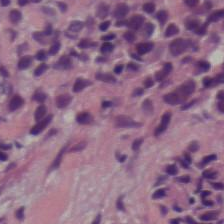
\includegraphics[width=\textwidth]{figures/ejemplos_clase/parches/her2_01plus}
\caption{0/1+}
\end{subfigure}\hfill
\begin{subfigure}[b]{0.3\textwidth}
\centering
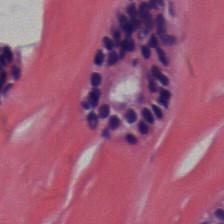
\includegraphics[width=\textwidth]{figures/ejemplos_clase/parches/her2_2plus}
\caption{2+}
\end{subfigure}\hfill
\begin{subfigure}[b]{0.3\textwidth}
\centering
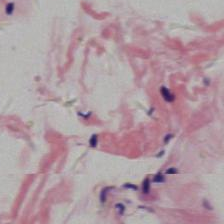
\includegraphics[width=\textwidth]{figures/ejemplos_clase/parches/her2_3plus}
\caption{3+}
\end{subfigure}
\caption{Ejemplos representativos de parches para cada clase de HER2.}
\label{fig:ejemplos_her2}
\end{figure}

\paragraph{Desempeño por modelo y dataset.} En BCNB, la BA osciló entre 0,418 (Phikon-v2) y 0,455 (UNI2), con AUC macro entre 0,602 y 0,632: todos los modelos superan el nivel de referencia de 0,333 correspondiente a tres clases, aunque con una ganancia limitada. En HISTAI-Breast el desempeño desciende a 0,364--0,381, también cercano al nivel de referencia. En HSI-BC, donde solo están presentes dos clases y el nivel de referencia es 0,5, UNI2 (0,438), Virchow2 (0,417) y Phikon-v2 (0,278) quedan por debajo de él, mientras que Prov-GigaPath alcanza 0,562 con IC95\% de [0,359, 0,762]; la amplitud de este intervalo, junto con el tamaño de cohorte de $n=44$, impide establecer una ventaja concluyente (Figura~\ref{fig:ba_her2}).

El análisis por clase muestra una marcada heterogeneidad. En las cohortes grandes, la categoría 2+ es la mejor detectada (sensibilidad de 0,573--0,625 en BCNB y 0,709--0,747 en HISTAI-Breast), en línea con su condición de clase mayoritaria (45,7\% y 63,2\% de los casos, respectivamente), mientras que 0/1+ y 3+ se detectan de forma deficiente (0,140--0,403). En HSI-BC, Virchow2 y Phikon-v2 no identifican ningún caso de 3+ (sensibilidad 0,000), aunque esta observación se basa en un número reducido de pacientes. El AUC es coherente con este patrón: sobre HSI-BC, UNI2 (0,389) y Phikon-v2 (0,184) presentan valores por debajo del azar, lo que, dado el reducido tamaño de la cohorte, indica ausencia de señal aprendida o ruido muestral extremo. Los valores numéricos completos se presentan en las Tablas~\ref{tab:anexo_her2_utilidad}, \ref{tab:anexo_her2_sensibilidad}--\ref{tab:anexo_her2_sensibilidad_hsibc}, \ref{tab:anexo_her2_fairness}--\ref{tab:anexo_her2_fairness_hsibc} y \ref{tab:anexo_her2_crossdataset} del Apéndice~\ref{anexo:resultados_completos}.

\begin{figure}[htbp]
\centering
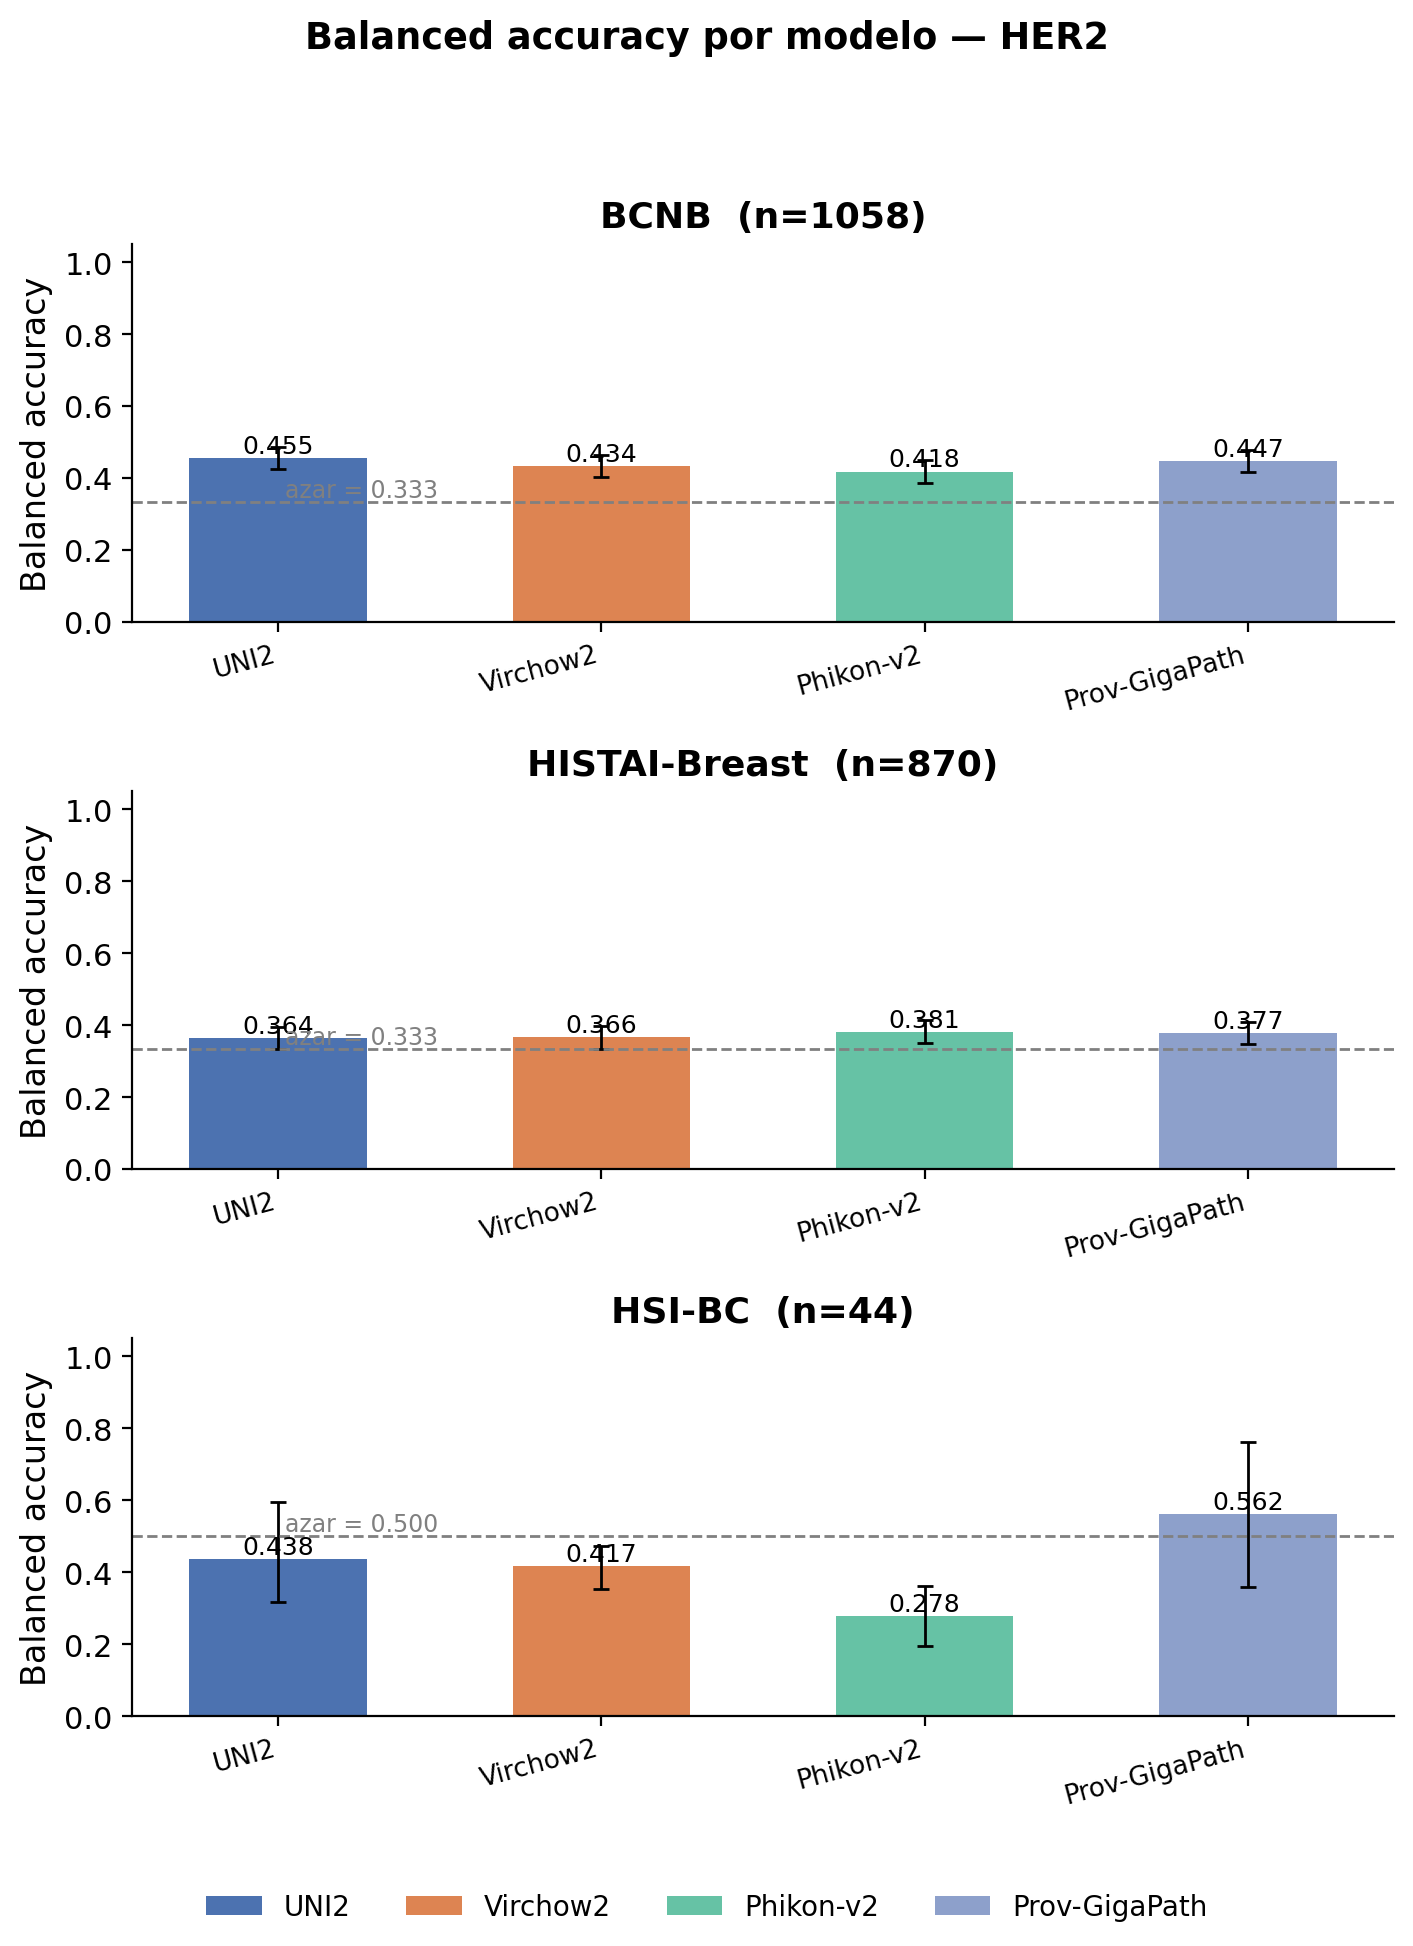
\includegraphics[width=0.75\textwidth]{figures/balanced_accuracy/her2}
\caption{Balanced accuracy por modelo y conjunto de datos en la tarea HER2. Barras de error: IC 95\% bootstrap.}
\label{fig:ba_her2}
\end{figure}

\paragraph{Equidad entre subgrupos.} En BCNB, las brechas de BA por edad variaron entre modelos: UNI2 y Phikon-v2 presentaron las brechas más altas (0,113 y 0,105, respectivamente, con el grupo de $\geq 70$ años como el de mayor desempeño y el de $<50$ años como el de menor), mientras que Virchow2 y Prov-GigaPath presentaron brechas menores (0,032 y 0,019). En HISTAI-Breast, las brechas oscilaron entre 0,022 y 0,065, pero la dirección de la diferencia no fue consistente entre encoders: el grupo de mayor desempeño varía según el modelo evaluado. En HSI-BC, solo los grupos de 50--70 y $\geq 70$ años cumplen el umbral mínimo de inclusión ($n=26$ y $n=14$); las brechas estimadas varían entre 0,003 y 0,123, pero los intervalos de confianza son amplios, por lo que los resultados deben considerarse exploratorios y no permiten inferir de manera robusta la presencia o ausencia de disparidad por edad. No se observó una dirección de favorecimiento consistente entre encoders en las cohortes grandes.

\paragraph{Generalización cross-dataset.} La transferencia BCNB $\rightarrow$ HISTAI-Breast redujo la BA en 0,075--0,108 (16,5--24,1\%), y la transferencia inversa en 0,031--0,055 (8,4--14,4\%). Este patrón es compatible con una mayor proximidad entre ambas cohortes que la observada respecto de HSI-BC; sin embargo, el diseño no permite atribuir esta diferencia exclusivamente a similitudes morfológicas, ya que pueden intervenir factores de adquisición, composición clínica, prevalencia de clases y calidad de las etiquetas. Las transferencias que involucran HSI-BC combinan un cambio de cohorte con un cambio en el número de clases efectivamente evaluadas (la cohorte no contiene la categoría 2+) y, por ello, no son directamente comparables con las transferencias entre BCNB e HISTAI-Breast. Cuando HSI-BC actúa como fuente de entrenamiento, algunos modelos presentan valores OOD superiores a sus valores ID (p.\ ej., $\Delta M = -0{,}249$ para Phikon-v2 al evaluar en BCNB); este resultado no debe interpretarse como generalización superior, sino como una consecuencia posible de la estimación inestable del desempeño ID en una cohorte pequeña y con dos clases.

\paragraph{Síntesis.} En conjunto, T1 muestra una utilidad predictiva limitada bajo el protocolo de extracción de características congeladas y clasificación a nivel de paciente utilizado en este estudio: incluso en las cohortes de mayor tamaño, la BA supera el nivel de referencia por un margen acotado y la sensibilidad se concentra en la categoría 2+. Este comportamiento es compatible con la relación indirecta entre la morfología H\&E y un biomarcador definido mediante inmunohistoquímica, así como con el efecto del desbalance de clases, aunque el diseño no permite separar la contribución de ambos factores. Las diferencias entre cohortes son coherentes con las limitaciones documentadas en el Capítulo~\ref{cap:caracterizacion_datasets}: BCNB presenta el desempeño más alto y estable; HISTAI-Breast alcanza resultados menores en un contexto donde la obtención de biomarcadores desde texto libre puede introducir incertidumbre de etiquetado; y HSI-BC concentra la mayor inestabilidad debido a su tamaño reducido y su limitada representación de clases. Respecto de la equidad, no se observa una dirección de favorecimiento consistente entre modelos y cohortes, por lo que los resultados constituyen una caracterización exploratoria de posibles disparidades, no evidencia definitiva de equidad o inequidad por edad.

\subsection{T2: Subtipo molecular}
\label{sec:resultado_molsub}

\paragraph{Descripción de la tarea y distribución de clases.} T2 clasifica el subtipo molecular del cáncer de mama en cuatro categorías: Luminal A, Luminal B, HER2+ y triple negativo. En BCNB ($n=1.058$) la distribución es relativamente equilibrada (Luminal B 35,2\%, Luminal A 27,2\%, HER2+ 25,8\%, triple negativo 11,8\%); en HISTAI-Breast ($n=842$) domina Luminal B (41,6\%) y triple negativo es minoritaria (8,8\%); en HSI-BC ($n=44$) Luminal B concentra el 63,6\% de los casos y HER2+ cuenta con solo tres casos. La Figura~\ref{fig:ejemplos_molsub} muestra parches ejemplares representativos de cada clase, y la Figura~\ref{fig:anexo_dist_molsub} del Apéndice~\ref{anexo:figuras_distribucion}, la distribución de clases por conjunto de datos.

\begin{figure}[htbp]
\centering
\begin{subfigure}[b]{0.45\textwidth}
\centering
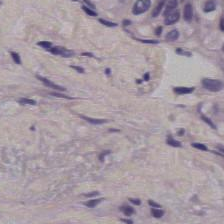
\includegraphics[width=\textwidth]{figures/ejemplos_clase/parches/molsub_her2plus}
\caption{HER2+}
\end{subfigure}\hfill
\begin{subfigure}[b]{0.45\textwidth}
\centering
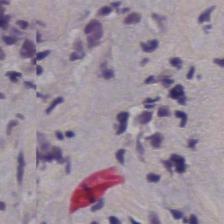
\includegraphics[width=\textwidth]{figures/ejemplos_clase/parches/molsub_luminal_a}
\caption{Luminal A}
\end{subfigure}
\\[2ex]
\begin{subfigure}[b]{0.45\textwidth}
\centering
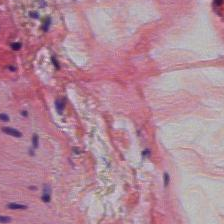
\includegraphics[width=\textwidth]{figures/ejemplos_clase/parches/molsub_luminal_b}
\caption{Luminal B}
\end{subfigure}\hfill
\begin{subfigure}[b]{0.45\textwidth}
\centering
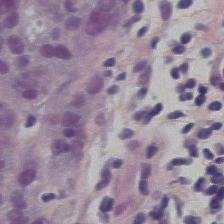
\includegraphics[width=\textwidth]{figures/ejemplos_clase/parches/molsub_triple_neg}
\caption{Triple Negative}
\end{subfigure}
\caption{Ejemplos representativos de parches para cada clase de MolSub.}
\label{fig:ejemplos_molsub}
\end{figure}

\paragraph{Desempeño por modelo y dataset.} BCNB presentó la mayor utilidad: UNI2 alcanzó la mayor BA (0,482; IC95\%: 0,450--0,514), seguido de Prov-GigaPath (0,472), Phikon-v2 (0,434) y Virchow2 (0,427), con AUC macro entre 0,697 y 0,740, superiores a los observados en T1 sobre la misma cohorte. Bajo el protocolo utilizado, este resultado indica una mayor capacidad discriminativa para T2 que para T1; sin embargo, la diferencia también puede estar influida por la definición de las etiquetas, su distribución y su calidad. En HISTAI-Breast, la BA disminuyó a 0,327--0,361. En HSI-BC, donde el nivel de referencia para cuatro clases es 0,25, UNI2 y Prov-GigaPath alcanzaron 0,317 y 0,334, mientras que Virchow2 y Phikon-v2 quedaron por debajo de este valor; dado que la cohorte contiene solo 44 pacientes y presenta categorías con escasa representación, estas diferencias deben interpretarse como estimaciones inestables y no como un ordenamiento concluyente entre modelos (Figura~\ref{fig:ba_molsub}).

El análisis por clase evidenció una heterogeneidad relevante. Luminal B fue la categoría con mayor sensibilidad en BCNB y en HISTAI-Breast (0,492--0,617); HER2+ presentó sensibilidades de 0,262--0,403 en las cohortes grandes; triple negativo alcanzó 0,448--0,568 en BCNB, pero disminuyó a 0,216--0,230 en HISTAI-Breast. En HSI-BC, ningún modelo identificó los tres casos de HER2+, por lo que esa sensibilidad igual a cero debe interpretarse principalmente en función del tamaño extremadamente reducido de la categoría. Los valores numéricos completos se presentan en las Tablas~\ref{tab:anexo_molsub_utilidad}, \ref{tab:anexo_molsub_sensibilidad}--\ref{tab:anexo_molsub_sensibilidad_hsibc}, \ref{tab:anexo_molsub_fairness}--\ref{tab:anexo_molsub_fairness_hsibc} y \ref{tab:anexo_molsub_crossdataset} del Apéndice~\ref{anexo:resultados_completos}.

\begin{figure}[htbp]
\centering
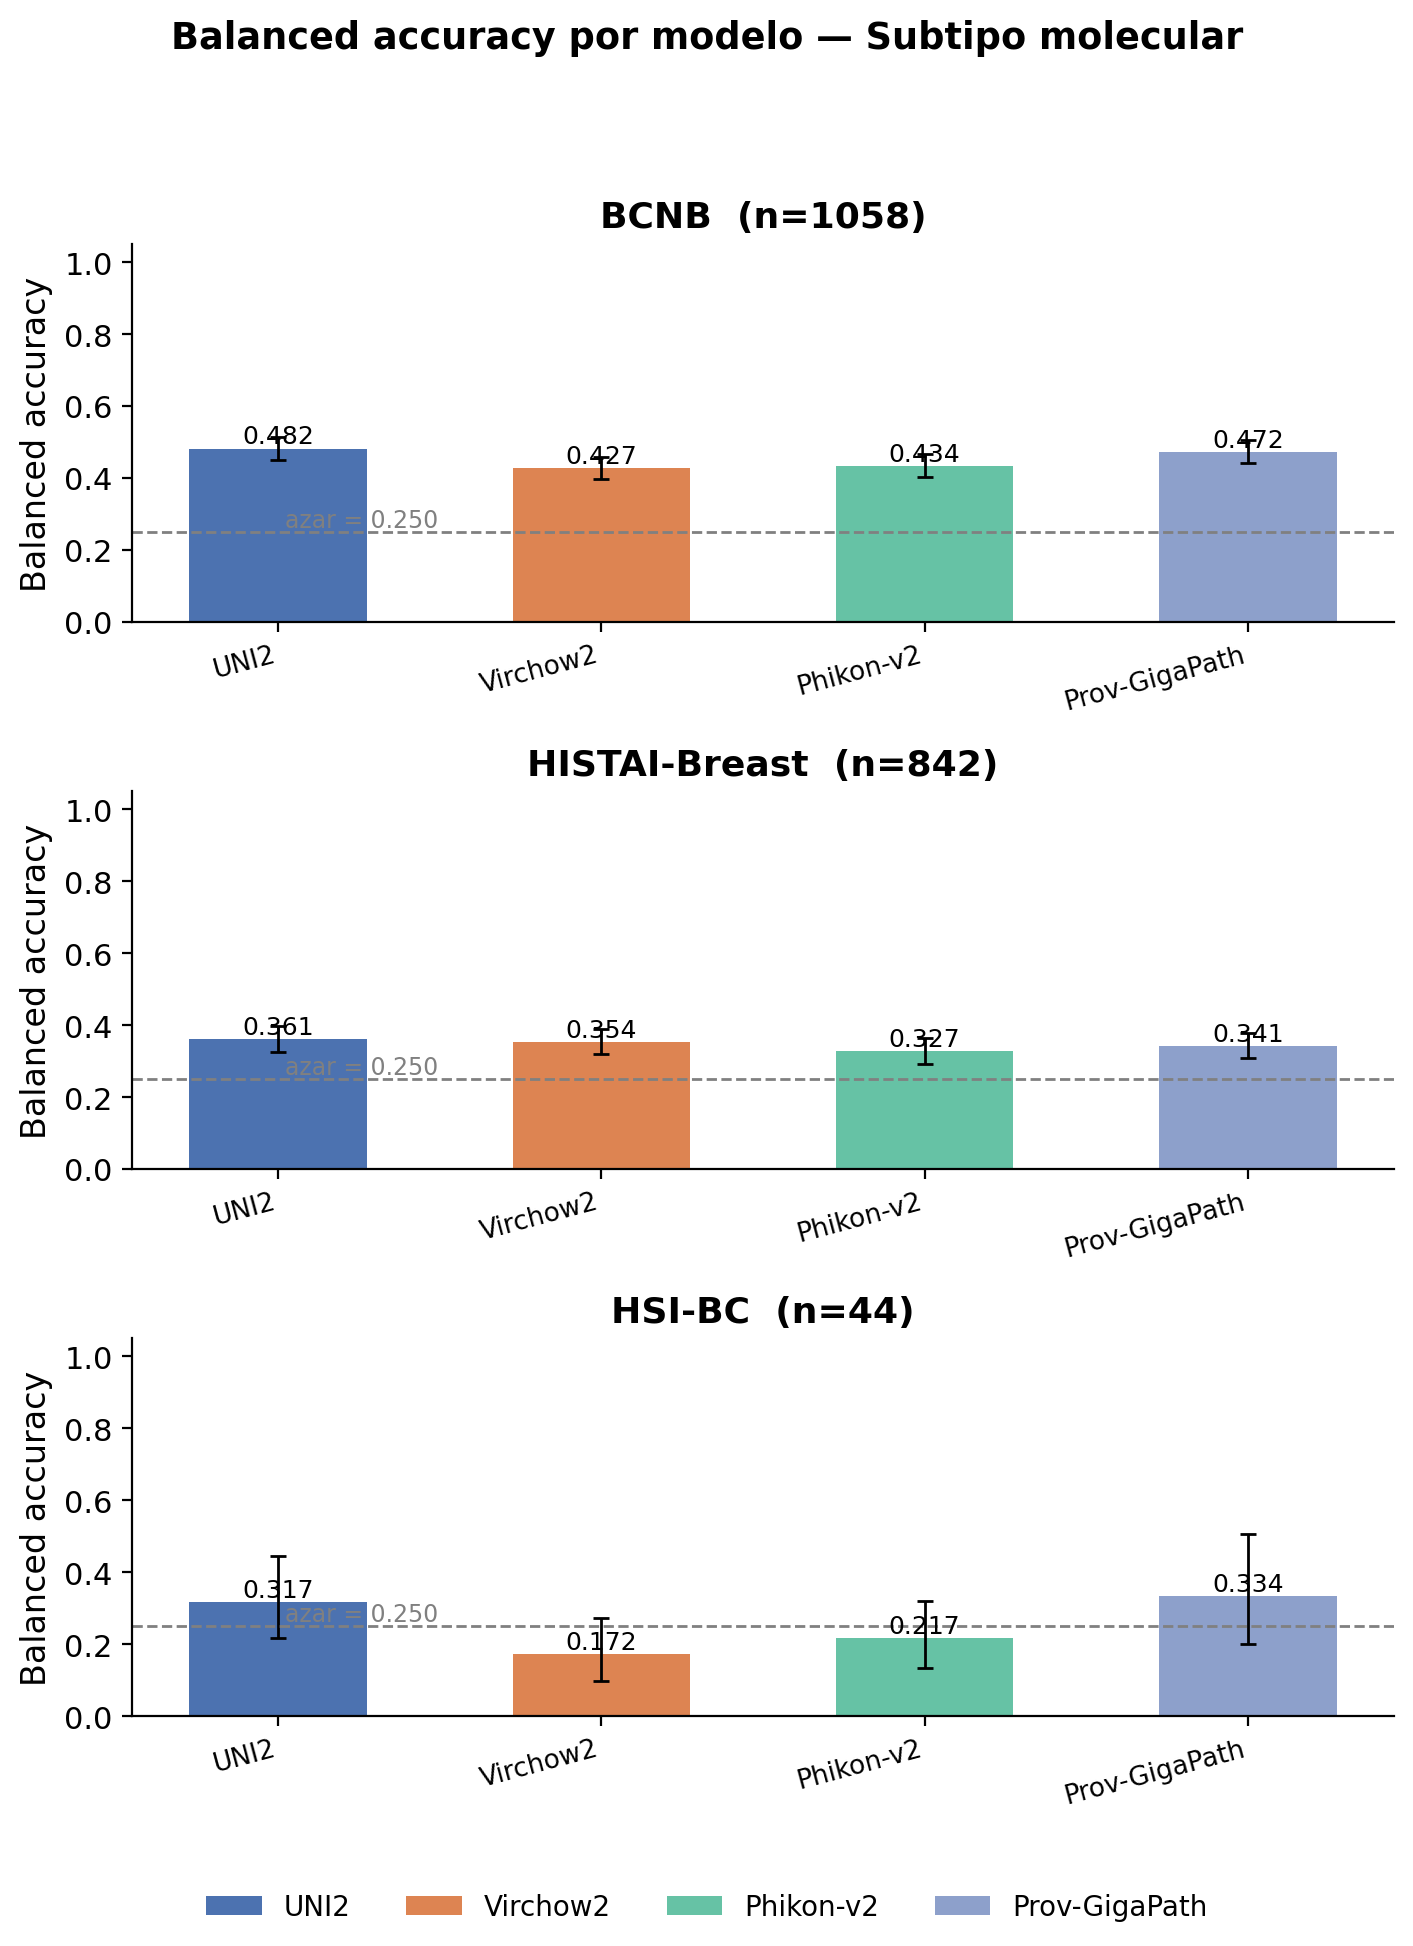
\includegraphics[width=0.72\textwidth]{figures/balanced_accuracy/molsub}
\caption{Balanced accuracy por modelo y conjunto de datos en la tarea MolSub. Barras de error: IC 95\% bootstrap.}
\label{fig:ba_molsub}
\end{figure}

\paragraph{Equidad entre subgrupos.} En BCNB, las brechas de BA por edad variaron entre modelos: Virchow2 y Phikon-v2 presentaron las brechas más bajas (0,010 y 0,023, respectivamente), mientras que UNI2 y Prov-GigaPath alcanzaron 0,078 y 0,041. La dirección de las diferencias no fue uniforme: el grupo de menor edad obtiene el mayor desempeño en UNI2, mientras que en Phikon-v2 el grupo de $\geq 70$ años registra el mayor desempeño; el grupo de $\geq 70$ años registra el menor desempeño en UNI2 y Prov-GigaPath. Por tanto, no se observa un grupo etario favorecido de manera consistente entre los cuatro modelos. En HISTAI-Breast, las brechas variaron entre 0,063 (UNI2) y 0,107 (Virchow2), con grupos de mejor desempeño que cambian según el modelo; estas diferencias deben interpretarse considerando el sesgo de selección hacia pacientes mayores en la cohorte analítica. En HSI-BC, las brechas variaron entre 0,074 y 0,426; la mayor correspondió a Prov-GigaPath, con BA de 0,593 en el grupo de 50--70 años y de 0,190 en el de $\geq 70$, sobre subgrupos de $n=26$ y $n=14$. Además, en cohortes pequeñas y tareas multiclase, la comparación de BA por subgrupo puede estar condicionada por la ausencia o escasa presencia de algunas categorías dentro de cada grupo etario. Por esta razón, las brechas reportadas describen diferencias observadas en esta muestra, pero no deben interpretarse como estimaciones estables de equidad poblacional.

\paragraph{Generalización cross-dataset.} La transferencia desde BCNB hacia HISTAI-Breast redujo la BA en 0,070--0,163, equivalentes a pérdidas relativas de 16,5\% a 34,6\%; la magnitud de la caída varió entre modelos: Virchow2 presentó la menor reducción, mientras que Prov-GigaPath y UNI2 registraron las mayores. Estos resultados indican una pérdida de rendimiento al trasladar el clasificador a una cohorte externa, aunque el diseño no permite separar la contribución de las diferencias de adquisición, composición clínica, prevalencia de subtipos y calidad de las etiquetas. La transferencia hacia HSI-BC presentó resultados más variables: UNI2 y Virchow2 registraron caídas de 0,253 y 0,205, Phikon-v2 de 0,108, y Prov-GigaPath una diferencia reducida de 0,004; este último resultado no debe interpretarse por sí solo como evidencia de robustez superior, ya que HSI-BC es una cohorte pequeña, con distribución de clases distinta y categorías muy escasas. Cuando HSI-BC se utilizó como conjunto de entrenamiento, algunos modelos presentaron valores OOD superiores a su desempeño ID (p.\ ej., $\Delta M = -0{,}096$ para Virchow2 al evaluar en BCNB), patrón compatible con la inestabilidad de la estimación ID en una cohorte pequeña. Los resultados completos se presentan en la Tabla~\ref{tab:anexo_molsub_crossdataset} del Apéndice~\ref{anexo:resultados_completos}.

\paragraph{Síntesis.} T2 presenta una utilidad predictiva mayor que T1 en BCNB, particularmente al considerar el AUC macro: bajo este protocolo, las representaciones fundacionales contienen información más útil para discriminar subtipos moleculares que para clasificar el estado HER2 aislado. Sin embargo, este resultado no permite concluir que la diferencia provenga exclusivamente de una señal morfológica más fuerte, dado que las tareas también difieren en definición de etiquetas, distribución de clases y posibles fuentes de incertidumbre en los metadatos clínicos, en especial la extracción de biomarcadores desde texto libre en HISTAI-Breast. El desempeño disminuye de forma consistente desde BCNB hacia HISTAI-Breast y, con mayor inestabilidad, hacia HSI-BC, un gradiente compatible con las limitaciones documentadas en la caracterización de las cohortes. Respecto de la equidad, no se observa un patrón de favorecimiento consistente entre modelos ni entre cohortes; la brecha elevada de Prov-GigaPath en HSI-BC requiere validación en una cohorte mayor. Los resultados caracterizan posibles disparidades bajo las condiciones evaluadas, pero no permiten afirmar de manera definitiva ni la presencia ni la ausencia de inequidad por edad.

\subsection{T3: Sitio anatómico}
\label{sec:resultado_site}

\paragraph{Descripción de la tarea y distribución de clases.} T3 clasifica el sitio anatómico del tumor colorrectal en nueve categorías: colon derecho, colon transverso, colon izquierdo, sigmoide, rectosigmoide, recto, colon sin especificar, otro y metástasis hepática. En HISTAI-CRC-B1 ($n=878$) predominan sigmoide (24,0\%), recto (18,2\%) y colon derecho (15,4\%); en SurGen ($n=765$) dominan recto (29,8\%) y colon derecho (22,9\%); en HISTAI-CRC-B2 ($n=57$) la clase metástasis hepática está ausente, por lo que la tarea se evalúa con ocho clases, y varias clases cuentan con menos de cinco casos (colon izquierdo 2, rectosigmoide 1, transverso 1). La Figura~\ref{fig:ejemplos_site} muestra parches ejemplares representativos de cada clase, y la Figura~\ref{fig:anexo_dist_site} del Apéndice~\ref{anexo:figuras_distribucion}, la distribución de clases por conjunto de datos.

\begin{figure}[htbp]
\centering
\begin{subfigure}[b]{0.3\textwidth}
\centering
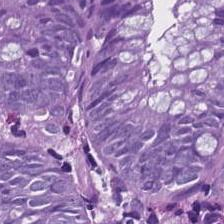
\includegraphics[width=\textwidth]{figures/ejemplos_clase/parches/site_colon_sin_especificar}
\caption{Colon sin especificar}
\end{subfigure}\hfill
\begin{subfigure}[b]{0.3\textwidth}
\centering
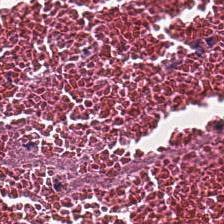
\includegraphics[width=\textwidth]{figures/ejemplos_clase/parches/site_colon_izquierdo}
\caption{Colon izquierdo}
\end{subfigure}\hfill
\begin{subfigure}[b]{0.3\textwidth}
\centering
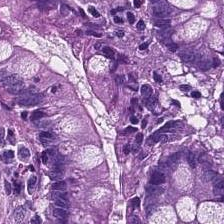
\includegraphics[width=\textwidth]{figures/ejemplos_clase/parches/site_met_higado}
\caption{Metástasis hepática}
\end{subfigure}
\\[2ex]
\begin{subfigure}[b]{0.3\textwidth}
\centering
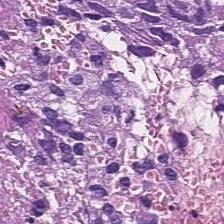
\includegraphics[width=\textwidth]{figures/ejemplos_clase/parches/site_otro}
\caption{Otro}
\end{subfigure}\hfill
\begin{subfigure}[b]{0.3\textwidth}
\centering
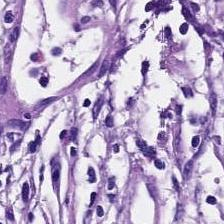
\includegraphics[width=\textwidth]{figures/ejemplos_clase/parches/site_rectosigmoide}
\caption{Rectosigmoide}
\end{subfigure}\hfill
\begin{subfigure}[b]{0.3\textwidth}
\centering
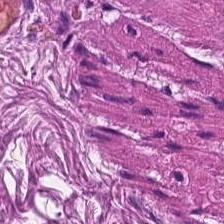
\includegraphics[width=\textwidth]{figures/ejemplos_clase/parches/site_recto}
\caption{Recto}
\end{subfigure}
\\[2ex]
\begin{subfigure}[b]{0.3\textwidth}
\centering
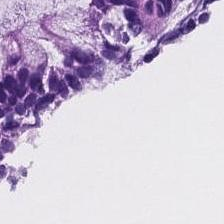
\includegraphics[width=\textwidth]{figures/ejemplos_clase/parches/site_colon_derecho}
\caption{Colon derecho}
\end{subfigure}\hfill
\begin{subfigure}[b]{0.3\textwidth}
\centering
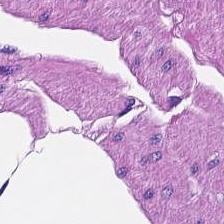
\includegraphics[width=\textwidth]{figures/ejemplos_clase/parches/site_sigmoide}
\caption{Sigmoide}
\end{subfigure}\hfill
\begin{subfigure}[b]{0.3\textwidth}
\centering
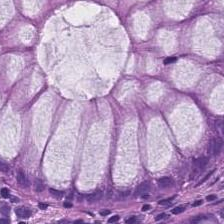
\includegraphics[width=\textwidth]{figures/ejemplos_clase/parches/site_colon_transverso}
\caption{Colon transverso}
\end{subfigure}
\caption{Ejemplos representativos de parches para cada clase de Site.}
\label{fig:ejemplos_site}
\end{figure}

\paragraph{Desempeño por modelo y dataset.} El nivel de referencia de la BA depende del número de clases presentes en cada cohorte: aproximadamente 0,111 para HISTAI-CRC-B1 y SurGen (nueve categorías) y 0,125 para HISTAI-CRC-B2 (ocho categorías). SurGen presentó el mayor desempeño absoluto, con BA de 0,309--0,367 (UNI2 = 0,367; IC95\%: 0,331--0,403); en HISTAI-CRC-B1 los cuatro modelos obtuvieron valores de 0,203--0,210, por sobre el nivel de referencia de una tarea con nueve clases; en HISTAI-CRC-B2, los valores variaron entre 0,094 y 0,138, cercanos al nivel de referencia de ocho clases y acompañados de intervalos de confianza amplios, por lo que esta cohorte no permite una estimación precisa de la utilidad predictiva de los modelos (Figura~\ref{fig:ba_site}).

La sensibilidad por clase fue heterogénea entre cohortes. En SurGen, recto, colon derecho y metástasis hepática alcanzaron máximos de 0,684, 0,480 y 0,886, respectivamente; en HISTAI-CRC-B1, colon derecho y sigmoide alcanzaron sensibilidades de 0,384--0,459, mientras que metástasis hepática no fue identificada por ninguno de los modelos a pesar de estar presente en 18 pacientes. El contraste entre la sensibilidad de metástasis hepática en SurGen y en HISTAI-CRC-B1 es compatible con una influencia de la frecuencia de la clase y de su representatividad dentro de cada cohorte, aunque las cohortes también difieren en adquisición, composición clínica y posibles criterios de anotación. Las categorías rectosigmoide y colon transverso mostraron sensibilidades bajas en las cohortes evaluadas, coherentes con su baja representación. Los valores numéricos completos se presentan en las Tablas~\ref{tab:anexo_site_utilidad}, \ref{tab:anexo_site_sensibilidad}--\ref{tab:anexo_site_sensibilidad_surgen}, \ref{tab:anexo_site_fairness_edad}--\ref{tab:anexo_site_fairness_edad_surgen}, \ref{tab:anexo_site_fairness_sexo}--\ref{tab:anexo_site_fairness_sexo_surgen} y \ref{tab:anexo_site_crossdataset} del Apéndice~\ref{anexo:resultados_completos}.

\begin{figure}[htbp]
\centering
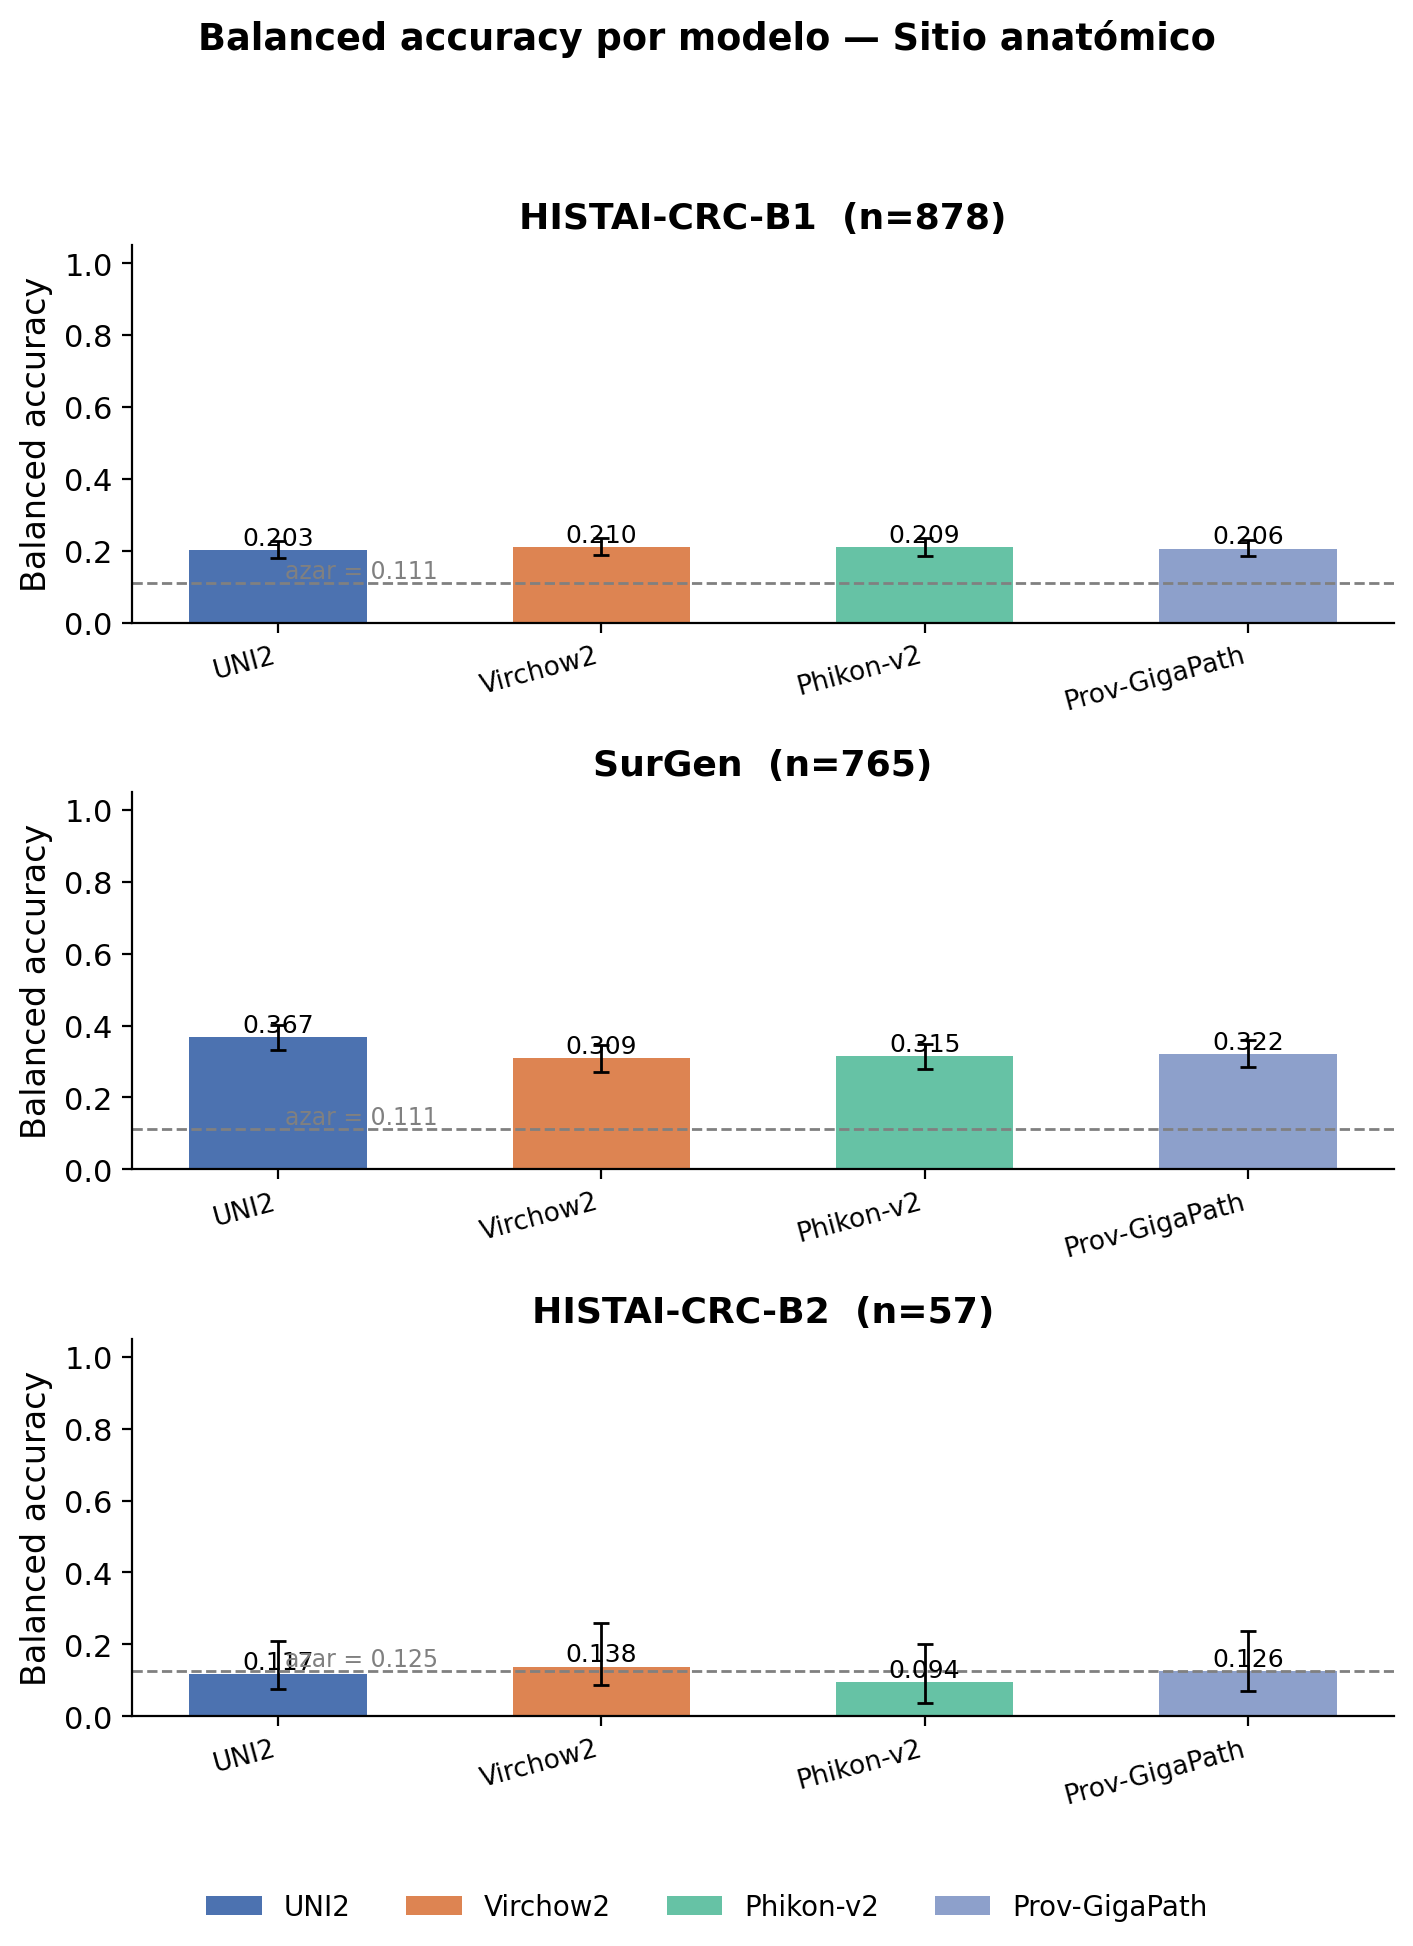
\includegraphics[width=0.72\textwidth]{figures/balanced_accuracy/site}
\caption{Balanced accuracy por modelo y conjunto de datos en la tarea Site. Barras de error: IC 95\% bootstrap.}
\label{fig:ba_site}
\end{figure}

\paragraph{Equidad entre subgrupos.} En las cohortes grandes, las brechas por edad fueron de magnitud reducida a moderada: entre 0,018 y 0,049 en HISTAI-CRC-B1 y entre 0,026 y 0,072 en SurGen. Las brechas por sexo también fueron acotadas en estas cohortes, con valores entre 0,026 y 0,046 en HISTAI-CRC-B1 y entre 0,002 y 0,063 en SurGen. La dirección de las diferencias varió entre modelos, por lo que no se observa un subgrupo de edad o sexo favorecido de manera consistente. En HISTAI-CRC-B2, los análisis por edad incluyeron únicamente los grupos de 50--70 y $\geq 70$ años ($n=25$ y $n=27$, respectivamente): las brechas estimadas variaron entre 0,053 y 0,360, con la mayor correspondiente a Phikon-v2 (IC95\%: [0,015, 0,778]); por sexo ($n=32$ mujeres y $n=25$ hombres), Phikon-v2 presentó una diferencia de 0,201, con BA de 0,201 en mujeres y 0,000 en hombres. Estas estimaciones deben interpretarse de forma exploratoria: el tamaño total de la cohorte es reducido, algunas categorías tienen muy pocos pacientes y la composición de clases puede diferir entre subgrupos, por lo que las diferencias observadas no permiten establecer de manera robusta si existe una disparidad real por edad o sexo.

\paragraph{Generalización cross-dataset.} La generalización entre cohortes colorrectales mostró caídas relevantes. Cuando SurGen actuó como conjunto de entrenamiento, la transferencia hacia HISTAI-CRC-B1 redujo la BA entre 0,166 y 0,238 (51,6--73,4\%), y hacia HISTAI-CRC-B2 entre 0,107 y 0,195, aunque esta última debe interpretarse con especial cautela por el tamaño reducido de la cohorte de destino y la ausencia de una de las categorías anatómicas. En la dirección HISTAI-CRC-B1 hacia SurGen, las caídas se situaron entre 0,081 y 0,106 (38,8--50,3\%). La asimetría entre direcciones muestra que la transferibilidad depende tanto de la cohorte de entrenamiento como de la de evaluación, resultado compatible con diferencias de distribución entre datasets, sin que el diseño permita identificar si estas provienen principalmente de factores técnicos, composición clínica, distribución de sitios anatómicos o procedimientos de anotación. Cuando HISTAI-CRC-B2 se utilizó como fuente de entrenamiento, algunos resultados OOD superaron el desempeño ID; dado que el desempeño ID de esta cohorte es cercano al nivel de referencia y se estima sobre solo 57 pacientes, los deltas negativos deben interpretarse como evidencia de inestabilidad de la estimación ID, no como una demostración de generalización externa. Los resultados completos se presentan en la Tabla~\ref{tab:anexo_site_crossdataset} del Apéndice~\ref{anexo:resultados_completos}.

\paragraph{Síntesis.} T3 es una tarea de alta complejidad: combina un número elevado de categorías anatómicas, distribuciones de clase asimétricas y clases con soporte muy reducido. Por ello, su BA debe interpretarse en relación con el nivel de referencia de una tarea de ocho o nueve clases, y no compararse de manera directa con las tareas binarias o de menor granularidad del capítulo. SurGen alcanza el mejor desempeño absoluto, HISTAI-CRC-B1 obtiene resultados moderados sobre el nivel de referencia, y HISTAI-CRC-B2 no proporciona evidencia suficiente para una evaluación estable de utilidad predictiva, equidad o generalización. La detección desigual de metástasis hepática entre SurGen e HISTAI-CRC-B1 ilustra que el desempeño por clase puede estar condicionado simultáneamente por prevalencia, representatividad de las muestras y diferencias entre cohortes. Respecto de la equidad, las cohortes grandes no muestran un patrón consistente de favorecimiento por edad o sexo; sin embargo, la utilidad predictiva global es limitada en esta tarea, por lo que brechas pequeñas no deben interpretarse por sí solas como evidencia de un desempeño equitativo clínicamente satisfactorio.

\subsection{T4: Lateralidad}
\label{sec:resultado_side}

\paragraph{Descripción de la tarea y distribución de clases.} T4 agrupa la localización del tumor colorrectal en cinco categorías: izquierdo, derecho, recto, rectosigmoide y transverso. En HISTAI-CRC-B1 ($n=615$) predominan izquierdo (39,7\%) y recto (26,0\%); en SurGen ($n=631$) la distribución es más equilibrada (recto 36,1\%, derecho 27,7\%, izquierdo 26,9\%); en HISTAI-CRC-B2 ($n=46$) las clases rectosigmoide y transverso cuentan con un caso cada una. La Figura~\ref{fig:ejemplos_side} muestra parches ejemplares representativos de cada clase, y la Figura~\ref{fig:anexo_dist_side} del Apéndice~\ref{anexo:figuras_distribucion}, la distribución de clases por conjunto de datos.

\begin{figure}[htbp]
\centering
\begin{subfigure}[b]{0.3\textwidth}
\centering
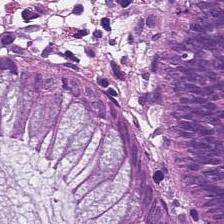
\includegraphics[width=\textwidth]{figures/ejemplos_clase/parches/side_izquierdo}
\caption{Izquierdo}
\end{subfigure}\hfill
\begin{subfigure}[b]{0.3\textwidth}
\centering
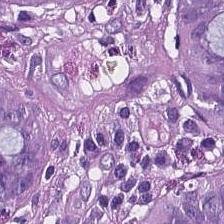
\includegraphics[width=\textwidth]{figures/ejemplos_clase/parches/side_rectosigmoide}
\caption{Rectosigmoide}
\end{subfigure}\hfill
\begin{subfigure}[b]{0.3\textwidth}
\centering
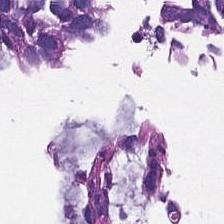
\includegraphics[width=\textwidth]{figures/ejemplos_clase/parches/side_recto}
\caption{Recto}
\end{subfigure}
\\[2ex]
\begin{minipage}{0.62\textwidth}
\centering
\begin{subfigure}[b]{0.48\textwidth}
\centering
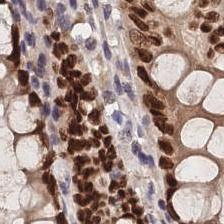
\includegraphics[width=\textwidth]{figures/ejemplos_clase/parches/side_derecho}
\caption{Derecho}
\end{subfigure}\hfill
\begin{subfigure}[b]{0.48\textwidth}
\centering
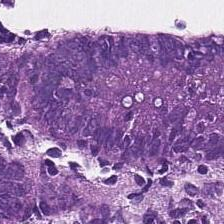
\includegraphics[width=\textwidth]{figures/ejemplos_clase/parches/side_transverso}
\caption{Transverso}
\end{subfigure}
\end{minipage}
\caption{Ejemplos representativos de parches para cada clase de Side.}
\label{fig:ejemplos_side}
\end{figure}

\paragraph{Desempeño por modelo y dataset.} La tarea comprende cinco categorías, por lo que el nivel de referencia uniforme de la BA corresponde a 0,2. En SurGen, UNI2 alcanzó la mayor BA (0,372; IC95\%: 0,329--0,415), seguido de Virchow2 (0,339), Phikon-v2 (0,321) y Prov-GigaPath (0,318); en HISTAI-CRC-B1, los resultados variaron entre 0,293 (Phikon-v2) y 0,331 (Prov-GigaPath). Ambas cohortes superan el nivel de referencia, aunque con una utilidad predictiva todavía moderada (Figura~\ref{fig:ba_side}). En HISTAI-CRC-B2, los cuatro modelos obtuvieron valores entre 0,115 y 0,174, inferiores al nivel de referencia; con solo 46 pacientes y dos categorías con un único caso, la BA y las sensibilidades por clase tienen una elevada variabilidad y no permiten establecer un ordenamiento confiable entre modelos.

El análisis por clase mostró diferencias relevantes entre cohortes: en HISTAI-CRC-B1, la categoría izquierdo presentó sensibilidades entre 0,607 y 0,660 y la categoría derecho entre 0,481 y 0,519; en SurGen, recto fue la categoría mejor detectada (0,675--0,737), seguida de derecho (0,434--0,560). En cambio, transverso y rectosigmoide presentaron sensibilidades bajas en las cohortes evaluadas, coherentes con su representación limitada. Los valores numéricos completos se presentan en las Tablas~\ref{tab:anexo_side_utilidad}, \ref{tab:anexo_side_sensibilidad}--\ref{tab:anexo_side_sensibilidad_surgen}, \ref{tab:anexo_side_fairness_edad}--\ref{tab:anexo_side_fairness_edad_surgen}, \ref{tab:anexo_side_fairness_sexo}--\ref{tab:anexo_side_fairness_sexo_surgen} y \ref{tab:anexo_side_crossdataset} del Apéndice~\ref{anexo:resultados_completos}.

\begin{figure}[htbp]
\centering
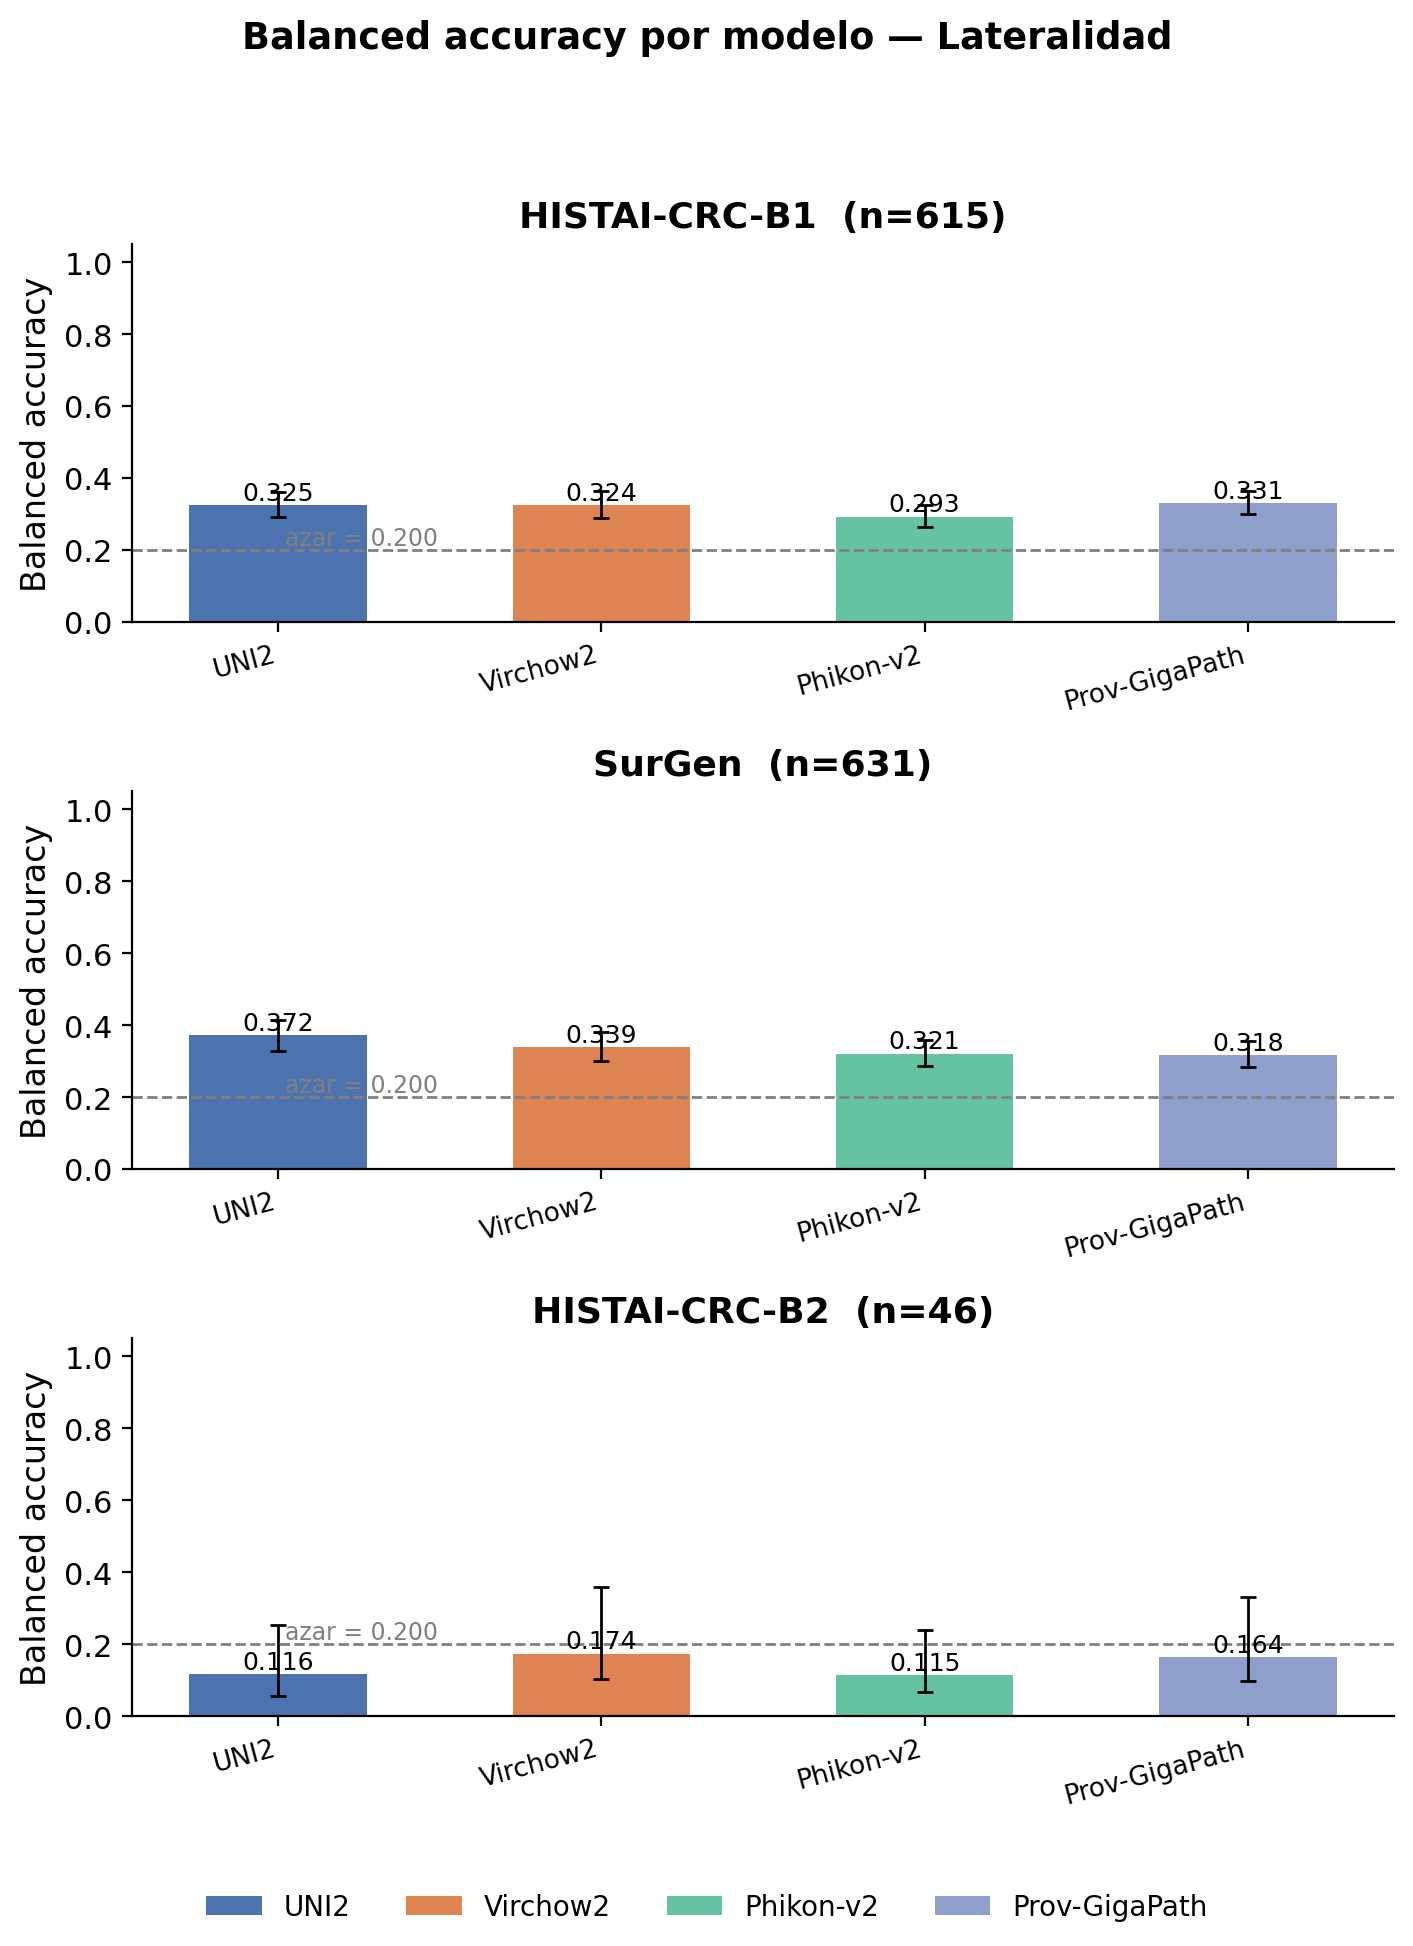
\includegraphics[width=0.72\textwidth]{figures/balanced_accuracy/side}
\caption{Balanced accuracy por modelo y conjunto de datos en la tarea Side. Barras de error: IC 95\% bootstrap.}
\label{fig:ba_side}
\end{figure}

\paragraph{Equidad entre subgrupos.} En HISTAI-CRC-B1, las brechas por edad variaron entre 0,028 y 0,074; en SurGen, entre 0,011 y 0,115 (Phikon-v2 presentó la mayor diferencia por edad y Prov-GigaPath la menor). Las brechas por sexo en las cohortes de mayor tamaño también fueron acotadas, con valores entre 0,032 y 0,061 en HISTAI-CRC-B1 y entre 0,024 y 0,057 en SurGen. La dirección de las diferencias cambia entre modelos, por lo que no se identifica un grupo de edad o sexo favorecido de manera consistente. En HISTAI-CRC-B2, los grupos de edad de 50--70 y $\geq 70$ años incluyen $n=21$ y $n=22$ pacientes: las brechas por edad variaron entre 0,076 y 0,193; por sexo, la cohorte incluye $n=26$ mujeres y $n=20$ hombres, con brechas entre 0,136 y 0,306 (Prov-GigaPath presentó la diferencia más alta, con BA de 0,373 en mujeres y de 0,067 en hombres). Las diferencias observadas en HISTAI-CRC-B2 deben interpretarse de manera exploratoria: en este contexto, una BA cercana a cero en un grupo no permite por sí sola concluir que exista sesgo por sexo o edad; se requiere una cohorte externa de mayor tamaño y con soporte suficiente por categoría para evaluar esa hipótesis.

\paragraph{Generalización cross-dataset.} La transferencia entre las cohortes colorrectales mostró caídas relevantes de rendimiento. Cuando SurGen actuó como conjunto de entrenamiento, la transferencia hacia HISTAI-CRC-B1 redujo la BA entre 0,085 y 0,166 (26,8--46,0\%); en la dirección inversa, desde HISTAI-CRC-B1 hacia SurGen, las caídas variaron entre 0,080 y 0,115 (24,6--39,1\%). La transferencia hacia HISTAI-CRC-B2 presentó mayor incertidumbre: UNI2 disminuyó 0,145 y Virchow2 0,205, mientras que Phikon-v2 y Prov-GigaPath presentaron diferencias pequeñas o negativas; dado que HISTAI-CRC-B2 contiene solo 46 pacientes y presenta categorías con soporte mínimo, estas diferencias no permiten comparar de forma confiable la robustez de los modelos frente a cambios de cohorte. Cuando HISTAI-CRC-B2 se utilizó como fuente de entrenamiento, se observaron nuevamente deltas negativos hacia HISTAI-CRC-B1, patrón compatible con una estimación ID inestable en una cohorte pequeña y con desempeño limitado. Los resultados completos se presentan en la Tabla~\ref{tab:anexo_side_crossdataset} del Apéndice~\ref{anexo:resultados_completos}.

\paragraph{Síntesis.} T4 presentó una utilidad predictiva mayor que T3 en las cohortes colorrectales de mayor tamaño, resultado compatible con la menor granularidad de la etiqueta (cinco categorías frente a nueve), aunque ambas tareas no contienen exactamente los mismos pacientes ni la misma distribución de clases. Los resultados por clase muestran que las categorías más representadas, izquierdo, derecho y recto, concentran las sensibilidades más altas, mientras que transverso y rectosigmoide mantienen sensibilidades bajas, patrón compatible con una influencia conjunta de la prevalencia de clases, la heterogeneidad morfológica y la definición de las categorías anatómicas. Respecto de la equidad, HISTAI-CRC-B1 y SurGen no muestran un patrón consistente de favorecimiento por edad o sexo, pero las brechas deben interpretarse junto con la utilidad predictiva global, que sigue siendo moderada; en HISTAI-CRC-B2, las diferencias por edad y sexo son exploratorias y no permiten confirmar ni descartar una disparidad real.

\subsection{T5: Órgano y separabilidad entre cohortes}
\label{sec:resultado_organ}
\label{sec:verificacion_center_effect}

\paragraph{Descripción de la tarea.} T5 clasifica el órgano de origen (mama vs.\ colorrectal) en los 3.675 pacientes integrados (para HSI-BC se usa su cohorte curada completa, $n=47$, pues la etiqueta de órgano está disponible en todos sus casos), con una distribución de 53,7\% para mama y 46,3\% para colorrectal. La tarea debe interpretarse como un experimento auxiliar de separabilidad entre cohortes: ninguna cohorte incluida contiene muestras de ambos órganos, por lo que la etiqueta de órgano está asociada al origen de la cohorte y el clasificador puede utilizar tanto diferencias entre tejidos como señales técnicas o institucionales asociadas al dataset, tales como tinción, escáner, preparación de la muestra o composición clínica.

\paragraph{Desempeño por modelo y dataset.} Los cuatro modelos resolvieron la tarea con desempeño casi perfecto: BA entre 0,996 (Prov-GigaPath) y 1,000 (Virchow2), AUC = 1,000 para los cuatro encoders, sensibilidad de 1,000 para mama en todos los casos y de 0,992--1,000 para colorrectal. Este resultado no debe interpretarse como una validación aislada de clasificación de órgano: demuestra la separabilidad de las cohortes integradas, no una capacidad de clasificación de órgano independiente de los factores de adquisición, institución, composición clínica, anotación y curación, que varían simultáneamente con el órgano. Las brechas por edad (0,000--0,010) están dominadas por un efecto de techo: cuando el desempeño es prácticamente perfecto para todos los grupos, la brecha de rendimiento queda limitada y aporta poca información sobre la capacidad del modelo para mantener un desempeño equitativo en una tarea clínicamente más exigente. La equidad por sexo no se evaluó debido a la cobertura incompleta de esta variable en la cohorte integrada. Los valores numéricos completos se presentan en las Tablas~\ref{tab:anexo_organ_utilidad}, \ref{tab:anexo_organ_sensibilidad} y \ref{tab:anexo_organ_fairness} del Apéndice~\ref{anexo:resultados_completos}.

\paragraph{Verificación experimental del \textit{center effect}.} Para evaluar directamente la señal de origen, se entrenaron clasificadores de dataset sobre los \textit{embeddings}, reutilizando la configuración del protocolo: MLP con 256 unidades ocultas y activación ReLU, $\alpha = 10^{-4}$, \texttt{max\_iter = 500}, sobremuestreo de las clases minoritarias y validación cruzada de cinco pliegues mediante \texttt{StratifiedGroupKFold}, agrupada por paciente y con \texttt{seed = 42}. El Experimento A evalúa la separabilidad entre datasets dentro de cada dominio clínico mediante clasificación de tres cohortes (nivel de referencia 1/3); el Experimento B compara pares de cohortes colorrectales (nivel de referencia 0,5). En el dominio de mama, BCNB, HISTAI-Breast y HSI-BC presentaron una separabilidad prácticamente perfecta dentro de la cohorte común de 1.944 pacientes utilizada en este experimento: los cuatro modelos alcanzaron BA y AUC de 1,000 para clasificar el dataset de origen. Este resultado muestra que los \textit{embeddings} contienen una firma de cohorte muy marcada; sin embargo, las tres cohortes difieren simultáneamente en institución, condiciones de adquisición, composición de pacientes, disponibilidad de metadatos y procesos de curación, por lo que esta comparación no permite atribuir la separación a un factor técnico o biológico específico.

El dominio colorrectal permite un contraste más informativo. HISTAI-CRC-B1 e HISTAI-CRC-B2 comparten el escáner Leica Aperio GT450 AT2, pero su origen sigue siendo altamente recuperable: la clasificación conjunta de SurGen, HISTAI-CRC-B1 e HISTAI-CRC-B2 alcanzó BA de 0,856--0,928 y AUC de 0,991--0,998; incluso HISTAI-CRC-B1 frente a HISTAI-CRC-B2 alcanzó BA de 0,821--0,864 y AUC de 0,970--0,986, mientras que los pares que incluyen SurGen (escáner diferente) alcanzaron BA y AUC de 1,000 (Tabla~\ref{tab:center_effect}). Esto muestra que existen diferencias entre cohortes que permanecen disponibles en las representaciones incluso cuando el escáner es compartido, posiblemente asociadas a tinción, preparación y manejo del tejido, distribución clínica, anotación, calidad de las imágenes u otros factores no observados; a la vez, la diferencia entre la separabilidad de B1 frente a B2 y la separabilidad perfecta de los pares que incluyen SurGen no permite cuantificar una contribución causal específica del escáner.

\begin{table}[htbp]
\centering
\caption{Resumen de la separabilidad entre cohortes mediante clasificación de origen de dataset. Los rangos de \textit{balanced accuracy} corresponden a los cuatro modelos fundacionales evaluados. El detalle completo se presenta en las Tablas~\ref{tab:anexo_center_effect_a} y \ref{tab:anexo_center_effect_b} del Apéndice~\ref{anexo:resultados_completos}.}
\label{tab:center_effect}
\small
\begin{tabular}{p{3.0cm} p{5.6cm} c c}
\toprule
\textbf{Dominio} & \textbf{Comparación} &
\textbf{$n_{\text{eval}}$} & \textbf{BA} \\
\midrule
Mama &
BCNB, HISTAI-Breast y HSI-BC &
1944 &
1.000 \\

Colorrectal &
SurGen, HISTAI-CRC-B1 e HISTAI-CRC-B2 &
1700 &
0.856 a 0.928 \\

Colorrectal &
HISTAI-CRC-B1 frente a HISTAI-CRC-B2, escáner compartido &
935 &
0.821 a 0.864 \\

Colorrectal &
SurGen frente a HISTAI-CRC-B1, escáner diferente &
1643 &
1.000 \\

Colorrectal &
SurGen frente a HISTAI-CRC-B2, escáner diferente &
822 &
1.000 \\
\bottomrule
\end{tabular}

\medskip
\footnotesize
\parbox{0.95\textwidth}{\textit{Nota:} La comparación de mama utiliza la cohorte común de 1944 pacientes disponible para los cuatro encoders, correspondiente a la cohorte analítica de T2-MOLSUB. Por ello, su tamaño difiere del reportado en T1-HER2.}
\end{table}

\paragraph{Síntesis.} Estos experimentos demuestran que el origen de la cohorte es altamente recuperable desde los \textit{embeddings} evaluados, hallazgo consistente con las caídas OOD observadas en T1--T4 y que refuerza la necesidad de interpretar tales caídas como el resultado potencial de múltiples fuentes de cambio de distribución. No permiten asignar causalmente esa separabilidad al escáner ni a un único factor, porque adquisición, institución, composición clínica, anotación y curación varían simultáneamente; el diseño actual no permite determinar qué proporción corresponde a diferencias morfológicas reales, factores técnicos de adquisición o características institucionales y clínicas de las cohortes. El detalle completo de las métricas e intervalos de confianza se presenta en las Tablas~\ref{tab:anexo_center_effect_a} y \ref{tab:anexo_center_effect_b} del Apéndice~\ref{anexo:resultados_completos}.

\section{Síntesis del capítulo}
\label{sec:sintesis_cap6}

La utilidad predictiva dependió principalmente de la tarea y de la cohorte. T2-MOLSUB superó a T1-HER2 en BCNB; en colorrectal, T4-SIDE obtuvo mayor utilidad que T3-SITE, coherente con su menor granularidad. T5-ORGAN fue casi perfecto, pero su interpretación está limitada por la confusión estructural entre órgano y origen de cohorte. La Tabla~\ref{tab:sintesis_utilidad_equidad} resume cualitativamente la utilidad predictiva, la estabilidad de las estimaciones de equidad y la generalización entre cohortes; los colores representan la interpretabilidad de los resultados bajo las condiciones de evaluación y no una clasificación definitiva de equidad, inequidad o sesgo.

\begin{table}[htbp]
\centering
\caption{Síntesis cualitativa de utilidad predictiva, equidad y generalización por tarea y cohorte. Los colores representan la estabilidad e interpretabilidad de los resultados, no una clasificación definitiva de sesgo o equidad.}
\label{tab:sintesis_utilidad_equidad}
\small
\resizebox{\textwidth}{!}{%
\begin{tabular}{l l p{3.2cm} p{3.6cm} p{3.4cm}}
\toprule
\textbf{Tarea} &
\textbf{Cohorte} &
\textbf{Utilidad predictiva} &
\textbf{Equidad por subgrupos} &
\textbf{Generalización} \\
\midrule

T1-HER2 &
BCNB &
\cellcolor{yellow!25}Limitada &
\cellcolor{yellow!25}Brechas variables por edad &
\cellcolor{yellow!25}Caída moderada hacia HISTAI-Breast \\

T1-HER2 &
HISTAI-Breast &
\cellcolor{yellow!25}Limitada &
\cellcolor{green!20}Sin patrón etario consistente &
\cellcolor{yellow!25}Caída moderada hacia BCNB \\

T1-HER2 &
HSI-BC &
\cellcolor{red!25}Exploratoria, $n=44$ &
\cellcolor{red!25}No concluyente &
\cellcolor{red!25}No interpretable de forma estable \\
\midrule

T2-MOLSUB &
BCNB &
\cellcolor{green!20}Mayor utilidad en mama &
\cellcolor{yellow!25}Brechas variables por edad &
\cellcolor{yellow!25}Caída hacia cohortes externas \\

T2-MOLSUB &
HISTAI-Breast &
\cellcolor{yellow!25}Moderada &
\cellcolor{yellow!25}Brechas variables por edad &
\cellcolor{yellow!25}Caída desde BCNB \\

T2-MOLSUB &
HSI-BC &
\cellcolor{red!25}Exploratoria, $n=44$ &
\cellcolor{red!25}No concluyente &
\cellcolor{red!25}No interpretable de forma estable \\
\midrule

T3-SITE &
HISTAI-CRC-B1 &
\cellcolor{yellow!25}Moderada para nueve clases &
\cellcolor{green!20}Sin patrón consistente &
\cellcolor{yellow!25}Caída relevante hacia SurGen \\

T3-SITE &
SurGen &
\cellcolor{green!20}Mayor utilidad de T3 &
\cellcolor{green!20}Sin patrón consistente &
\cellcolor{yellow!25}Caída relevante hacia otras cohortes \\

T3-SITE &
HISTAI-CRC-B2 &
\cellcolor{red!25}Exploratoria, $n=57$ &
\cellcolor{red!25}No concluyente &
\cellcolor{red!25}No interpretable de forma estable \\
\midrule

T4-SIDE &
HISTAI-CRC-B1 &
\cellcolor{yellow!25}Moderada &
\cellcolor{green!20}Sin patrón consistente &
\cellcolor{yellow!25}Caída hacia SurGen \\

T4-SIDE &
SurGen &
\cellcolor{green!20}Mayor utilidad de T4 &
\cellcolor{yellow!25}Brechas variables por edad &
\cellcolor{yellow!25}Caída hacia HISTAI-CRC-B1 \\

T4-SIDE &
HISTAI-CRC-B2 &
\cellcolor{red!25}Exploratoria, $n=46$ &
\cellcolor{red!25}No concluyente &
\cellcolor{red!25}No interpretable de forma estable \\
\midrule

T5-ORGAN &
Cohorte combinada &
\cellcolor{blue!20}Casi perfecta, pero confundida &
\cellcolor{blue!20}Efecto de techo &
\cellcolor{blue!20}No aplica \\
\bottomrule
\end{tabular}%
}

\medskip
\footnotesize
\parbox{0.97\textwidth}{\textit{Nota:} Verde indica resultados relativamente estables y sin un patrón demográfico consistente entre modelos. Amarillo indica resultados interpretables con limitaciones de utilidad, variabilidad entre modelos o caída de generalización. Rojo indica resultados exploratorios, condicionados por tamaño muestral reducido o soporte insuficiente de clases y subgrupos. Azul indica una dimensión no evaluable, no aplicable o dominada por confusión estructural. Los colores no constituyen una clasificación definitiva de equidad, inequidad o sesgo.}
\end{table}

No se identificó un patrón de favorecimiento por edad o sexo que fuese consistente entre encoders y cohortes grandes. Las brechas pequeñas no prueban por sí mismas equidad clínicamente satisfactoria cuando la utilidad global es limitada; las estimaciones de HSI-BC e HISTAI-CRC-B2 son exploratorias por tamaño y soporte de clases.

Las diferencias entre cohortes fueron más consistentes que las diferencias entre modelos fundacionales: ningún encoder dominó de manera transversal en todas las tareas y cohortes. BCNB, SurGen e HISTAI-CRC-B1 presentaron resultados más estables, mientras que HSI-BC e HISTAI-CRC-B2 concentraron la mayor incertidumbre debido a su tamaño reducido, la representación limitada de algunas clases y la menor estabilidad de las estimaciones; HISTAI-Breast presentó resultados intermedios, en un contexto donde la disponibilidad y trazabilidad de biomarcadores constituye una fuente adicional de incertidumbre.

La transferencia entre cohortes produjo caídas relevantes y el origen de dataset fue altamente separable desde los \textit{embeddings}. En consecuencia, la evaluación de modelos fundacionales en patología debe interpretar conjuntamente la tarea clínica, la calidad y trazabilidad de las cohortes, la estabilidad de las métricas por subgrupo y el cambio de distribución entre centros.
	\chapter{Conclusiones}
\label{cap:conclusiones}

Esta investigación abordó el problema del \textit{bias} y la \textit{fairness} en modelos fundacionales aplicados a \textit{Whole Slide Images} (WSI) de patología digital. El trabajo se sustentó en la premisa de que el buen desempeño agregado de estos modelos no basta para establecer su utilidad clínica: es necesario examinar la composición, procedencia y documentación de los datos, así como su comportamiento ante subgrupos y cambios de distribución. A partir del marco teórico y del estado del arte, se estableció que la variabilidad de las WSI, asociada a la población, los protocolos de preparación, la tinción, la digitalización y la institución de origen, puede afectar la transferencia de las representaciones aprendidas y ocultar disparidades que no son visibles mediante métricas globales \parencite{Basak2023,NEURIPS2024_c9826b9e}.

En respuesta a esta problemática, se revisaron y sistematizaron nueve recursos públicos de patología digital y se construyó un marco operativo para identificar indicadores observables de tres mecanismos potenciales de \textit{bias}: representación, adquisición, y documentación y selección. Posteriormente, se priorizaron seis cohortes de los dominios de cáncer de mama y colorrectal, para las cuales fue posible armonizar variables clínicas, demográficas y técnicas suficientes para definir espacios de evaluación comparables. Sobre esta base, se seleccionaron los modelos Phikon-v2, UNI2-h, Prov-GigaPath y Virchow2 como extractores de representaciones congelados, y se definieron cinco tareas de clasificación orientadas a examinar utilidad predictiva, desempeño por subgrupo y generalización entre cohortes. De este modo, la principal contribución metodológica del estudio consiste en vincular explícitamente la auditoría de los datos con un protocolo de evaluación homogéneo para modelos fundacionales de patología digital.

\paragraph{Objetivo general} El objetivo general, orientado a evaluar distintos niveles de \textit{bias} en modelos fundacionales clínicos mediante una caracterización sistemática de conjuntos de datos de WSI en términos de \textit{fairness} y \textit{bias}, se considera cumplido de manera parcial y en etapa de consolidación. Se completó la construcción de la base conceptual, la caracterización de las cohortes, la selección justificada de modelos y el diseño del protocolo experimental que articula desempeño global, brechas por subgrupo y generalización entre conjuntos de datos. Esta aproximación es coherente con la literatura que advierte que las métricas agregadas pueden ocultar diferencias relevantes entre grupos y que la evaluación de modelos fundacionales debe considerar simultáneamente utilidad y equidad \parencite{NEURIPS2024_c9826b9e}. La evaluación empírica desarrollada en el Capítulo~6 confirma esta aproximación: el riesgo de \textit{bias} documentado por dataset en la Tabla~\ref{tab:matriz_riesgo_unificada} predijo, de forma más consistente que la elección de modelo fundacional, tanto el nivel de utilidad alcanzado como la estabilidad de las conclusiones de equidad en las cinco tareas evaluadas (Sección~\ref{sec:sintesis_cap6}). Por lo tanto, el objetivo general se considera cumplido: se logró evaluar sistemáticamente distintos niveles de \textit{bias} en modelos fundacionales clínicos, articulando la caracterización de datos con un protocolo experimental común.

\paragraph{Objetivo específico 1} El primer objetivo específico, consistente en caracterizar conjuntos de datos de imágenes médicas de patología digital mediante la identificación de variables demográficas y parámetros de adquisición críticos para el estudio de \textit{bias}, se considera cumplido. La revisión de nueve recursos públicos permitió evidenciar una marcada heterogeneidad en tamaño de cohorte, estructura y completitud de metadatos. Tras el proceso de curación y armonización, se identificó que la edad constituye el atributo demográfico más viable para el análisis estratificado en los dominios seleccionados, mientras que el sexo no es utilizable como atributo sensible en cáncer de mama debido a la homogeneidad casi absoluta de las cohortes. Asimismo, se observó una asociación estructural entre la cohorte de origen y los parámetros técnicos de adquisición, tales como escáner, magnificación y tinción, lo cual limita la atribución de diferencias de desempeño exclusivamente a las variables clínicas. Este hallazgo es consistente con la evidencia que señala que la procedencia institucional puede dejar firmas visuales en imágenes histopatológicas y favorecer el aprendizaje de señales ajenas a la morfología de interés \parencite{alsaafin2023biased,howard2021site}. La caracterización desarrollada no demuestra por sí sola una brecha de \textit{fairness}, pero establece las condiciones necesarias para interpretar con cautela los resultados experimentales posteriores.

\paragraph{Objetivo específico 2} El segundo objetivo específico, referido a seleccionar modelos fundacionales representativos y definir tareas específicas acordes con los conjuntos de datos analizados, se considera cumplido. La selección de Phikon-v2, UNI2-h, Prov-GigaPath y Virchow2 se fundamentó en criterios de pertinencia para patología computacional, compatibilidad con WSI teñidas con hematoxilina y eosina, accesibilidad de pesos e implementación, documentación técnica, trazabilidad del preentrenamiento, diversidad metodológica y viabilidad computacional. Al emplear los cuatro modelos como extractores de representaciones congelados y mantener constante el procesamiento posterior, el protocolo reduce la influencia de adaptaciones específicas y favorece una comparación controlada de las representaciones preentrenadas. Además, la definición de tareas de clasificación de estado HER2, subtipo molecular, sitio anatómico, lateralidad y órgano permite examinar escenarios clínicos y anatómicos con distintos niveles de comparabilidad entre cohortes. Esta decisión se alinea con la literatura sobre modelos fundacionales en patología, que destaca la transferibilidad de representaciones auto-supervisadas, pero también la necesidad de evaluar sus supuestos de preentrenamiento y trazabilidad \parencite{chen2024uni,filiot2024phikonv2,xu2024provgigapath,vorontsov2024virchow}.

\paragraph{Objetivo específico 3} El tercer objetivo específico, correspondiente a evaluar el desempeño de los modelos seleccionados mediante métricas acordes con las tareas definidas y analizar el impacto del \textit{bias} sobre su capacidad de generalización, se encuentra en desarrollo. El protocolo ya establece una evaluación a nivel de paciente que incluye métricas de utilidad global, análisis por clase, brechas entre subgrupos, experimentos \textit{cross-dataset} e intervalos de confianza obtenidos mediante \textit{bootstrap} no paramétrico. Este diseño permite distinguir entre desempeño promedio, estabilidad de las estimaciones y variación asociada al cambio de cohorte, evitando interpretar una única métrica agregada como evidencia suficiente de robustez o equidad. De esta forma, se evaluaron cuatro modelos fundacionales en cinco tareas de clasificación, reportando utilidad global, brechas por subgrupo etario y de sexo, y generalización \textit{cross-dataset} con intervalos de confianza por \textit{bootstrap}. Las caídas de desempeño ante cambio de distribución fueron sustanciales y transversales (16--73\% de pérdida relativa en T1--T4), y el experimento dedicado de verificación del \textit{center effect} (Sección~\ref{sec:verificacion_center_effect}) cuantificó que una parte sustancial de estas caídas es atribuible a la firma de adquisición e institución, y no exclusivamente a un cambio morfológico real. El objetivo específico 3 se considera, por tanto, cumplido.

\paragraph{Hipótesis de investigación} La hipótesis planteó que los conjuntos de datos de imágenes médicas presentan \textit{bias} demográficos y de adquisición significativos, los cuales afectan negativamente la capacidad de generalización de modelos fundacionales para WSI y producen diferencias de desempeño entre subgrupos poblacionales. La evidencia disponible permite respaldar parcialmente su primer componente: la caracterización identificó desbalances de representación, restricciones de cobertura de metadatos y heterogeneidad técnica sistemáticamente asociada a las cohortes. Estos antecedentes son compatibles con mecanismos de \textit{bias} de representación y adquisición, y con el riesgo de \textit{domain shift} y \textit{shortcut learning} descrito en la literatura \parencite{suresh2021framework,mehrabi2021survey,geirhos2020shortcut,stacke2021domainshift}. Así, los sesgos de representación y adquisición documentados a lo largo del proyecto afectan la generalización, tal como confirma el experimento de verificación del \textit{center effect} (BA$\approx$0.85 entre cohortes de mismo escáner, BA=1.000 al introducir un escáner distinto), pero no respalda el segundo componente en las cohortes de tamaño adecuado: las brechas de equidad por edad y sexo fueron bajas y sin un grupo sistemáticamente desfavorecido en BCNB, HISTAI-Breast, SurGen y HISTAI-CRC-B1 ($<$0.10 en la mayoría de los casos). Las brechas elevadas observadas en HSI-BC e HISTAI-CRC-B2 no permiten distinguirse de ruido muestral dado el tamaño de esas cohortes y la amplitud de sus intervalos de confianza. En consecuencia, la hipótesis se considera aceptada parcialmente: se confirma que existen sesgos de adquisición con efecto medible sobre la generalización, pero no se encuentra evidencia de disparidades de desempeño sistemáticas entre subgrupos demográficos dentro del rango de datos evaluado.

\paragraph{Trabajo futuro}

El principal aprendizaje metodológico de este trabajo es que la evaluación de fairness y generalización en modelos fundacionales no depende únicamente de la elección del encoder, de la tarea predictiva o de las métricas empleadas. Depende de las características y limitaciones de los conjuntos de datos disponibles. La curación y armonización realizadas permitieron construir escenarios comparables para cáncer de mama y colorrectal; sin embargo, también evidenciaron que gran parte de los conjuntos de datos públicos de patología digital presenta documentación heterogénea, cobertura incompleta de variables clínicas y demográficas, tamaños muestrales desiguales y condiciones de adquisición estrechamente asociadas a cada cohorte.

Por otra parte, las diferencias de generalización entre cohortes no pueden atribuirse de forma aislada a un único factor. Cada dataset reúne simultáneamente variaciones en institución de origen, escáner, preparación de la muestra, protocolo de tinción, población clínica, criterios de anotación y proceso de curación de metadatos. La alta separabilidad del origen de las cohortes observada en los embeddings confirma que los modelos retienen información asociada al dataset; sin embargo, no permite determinar qué proporción de esta señal corresponde a características técnicas, clínicas o morfológicas reales.

A partir de ello, una línea de trabajo futuro prioritaria consiste en ampliar la disponibilidad y calidad de los datos antes de proponer mecanismos de mitigación a nivel de modelo. Sería especialmente valioso contar con cohortes multicéntricas que reporten de manera sistemática variables demográficas, atributos clínicos, detalles de adquisición, procedimientos de tinción, escáner utilizado y criterios de anotación. Además, sería necesario incorporar muestras que permitan desacoplar parcialmente estas fuentes de variación; por ejemplo, cohortes provenientes de distintas instituciones que compartan protocolos técnicos, o muestras obtenidas con distintos escáneres dentro de una misma institución.

También sería relevante evaluar los modelos sobre cohortes de mayor tamaño y con una representación más equilibrada de subgrupos demográficos y clases clínicas. Esto permitiría estimar métricas de fairness con menor incertidumbre, analizar posibles intersecciones entre atributos, por ejemplo, edad y sexo, y estudiar si las brechas se mantienen al modificar la composición de la población evaluada. En este contexto, la falta de una disparidad consistente en las cohortes analizadas no debe interpretarse como demostración de equidad clínica, sino como evidencia de que las diferencias observables están condicionadas por el soporte y la calidad de los datos disponibles.

Finalmente, se podrían evaluar estrategias de adaptación o mitigación, tales como normalización de tinción, adaptación de dominio, fine-tuning supervisado o aprendizaje federado \citep{Xu2025StainNormalization,Kumari2024DomainAdaptation,Zhang2024FederatedLearning}. No obstante, estas estrategias deberían evaluarse sobre datos suficientemente documentados y bajo escenarios externos bien definidos.
	
	% ----------------------------------------------------------
	% ----------- TERCERA PARTE --------------------------------
	% ### Bibliografía de este documento ###
	% La opción heading la coloca en la tabla de contenidos
	\printbibliography[heading=bibintoc]
	

	\printglossary[title=Glosario,toctitle=Glosario]

	% Alternativa de apéndices
	\appendix
	\chapter{Carta Gantt}
\label{appendix:carta}

Carta Gantt con planificación semana a semana para llevar a cabo el desarrollo del proyecto de tesis. Se especifican tareas junto a sus repectivas horas hombre.

\begin{figure}[htb]
\centering
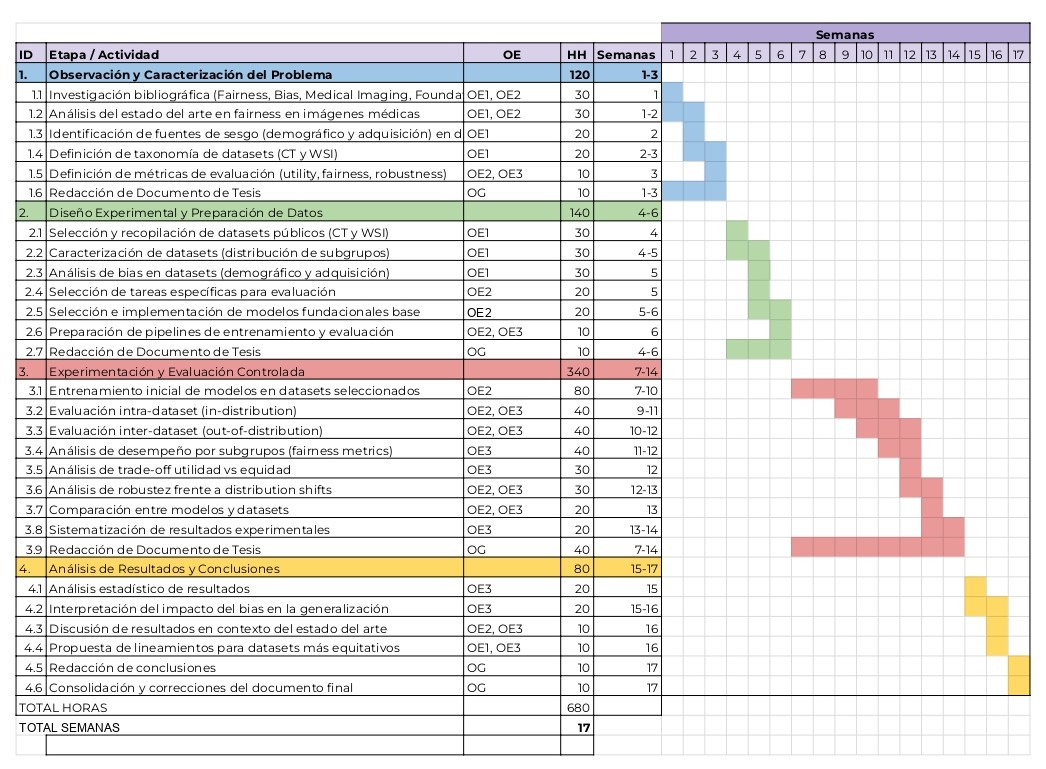
\includegraphics[width=1\textwidth]{images/cartagant.jpg}
\caption{Carta Gantt}
\end{figure}
	\chapter{Metadatos Reportados por los Conjuntos de Datos Analizados}
\label{appendix:tablasdatasets}

En este anexo se presentan las tablas resumidas de parámetros, variables y metadatos reportados por cada uno de los conjuntos de datos seleccionados en el Capítulo 4. Su objetivo es complementar la caracterización global de los datasets, proporcionando un detalle estructurado de los atributos clínicos, demográficos, diagnósticos, moleculares y de seguimiento disponibles en cada recurso. Adicionalmente, se incluyen la síntesis global de los recursos revisados con su desenlace en la preselección, las variables con mayor porcentaje de valores faltantes por dataset y los desgloses completos de frecuencias de las variables armonizadas en los dominios de mama y colorrectal; las versiones resumidas de estas tablas y su interpretación se presentan en el Capítulo~\ref{cap:caracterizacion_datasets}.

\begin{table}[ht]
\centering
\caption{Parámetros reportados por BCNB}
\label{tab:parametros_bcnb}
\renewcommand{\arraystretch}{1.2}
\begin{tabularx}{\textwidth}{lX}
\toprule
\textbf{Categoría} & \textbf{Variables reportadas} \\
\midrule
Identificación & Patient ID \\
Demográficas & Age(years) \\
Clínico-patológicas & Tumour Size(cm), Tumour Type, Histological grading, Number of lymph node metastases, ALN status \\
Biomarcadores / moleculares & ER, PR, HER2, HER2 Expression, Ki67, Molecular subtype \\
Tratamiento & Surgical \\
\bottomrule
\end{tabularx}
\end{table}

\begin{table}[ht]
\centering
\caption{Parámetros reportados por CLWD}
\label{tab:parametros_clwd}
\renewcommand{\arraystretch}{1.2}
\begin{tabularx}{\textwidth}{lX}
\toprule
\textbf{Categoría} & \textbf{Variables reportadas} \\
\midrule
Identificación & SampleNumber, WSI\_ID \\
Demográficas & Sex, Age \\
Clínico-patológicas & Pathological\_Diagnosis, Pathological\_Subspecies, Multi\_Subtypes, WHO2015\_GrowthPattern, WHO2021\_GrowthPattern, WHO2021\_category, WHO2021\_MucinousStatus \\
Etiquetas derivadas & Benchmark\_Label\_7class, Benchmark\_Label\_2021\_6class \\
\bottomrule
\end{tabularx}
\end{table}

\begin{table}[ht]
\centering
\caption{Parámetros reportados por NDB-UFES}
\label{tab:parametros_ndbufes}
\renewcommand{\arraystretch}{1.2}
\begin{tabularx}{\textwidth}{lX}
\toprule
\textbf{Categoría} & \textbf{Variables reportadas} \\
\midrule
Identificación & public\_id, lesion\_id, patient\_id, path \\
Demográficas & gender, skin\_color, age\_group \\
Clínico-patológicas & localization, larger\_size, diagnosis, dysplasia\_severity \\
Exposición / factores de riesgo & tobacco\_use, alcohol\_consumption, sun\_exposure \\
Tareas derivadas & TaskII, TaskIII, TaskIV \\
\bottomrule
\end{tabularx}
\end{table}

\begin{table}[ht]
\centering
\caption{Parámetros reportados por \textit{The Digital Brain Tumour Atlas}}
\label{tab:parametros_tdbta}
\renewcommand{\arraystretch}{1.2}
\begin{tabularx}{\textwidth}{lX}
\toprule
\textbf{Categoría} & \textbf{Variables reportadas} \\
\midrule
Identificación & uuid, pat\_id \\
Demográficas & age, sex \\
Clínico-patológicas & diagnosis, grade, subtype, secondary\_diagnosis, control, location, laterality, cellularity, tissue\_area \\
Desenlace / seguimiento & recurrence \\
Información adicional & comment \\
\bottomrule
\end{tabularx}
\end{table}

\begin{table}[ht]
\centering
\caption{Parámetros reportados por SurGen, diferenciando sus subcohortes SR386 y SR1482}
\label{tab:parametros_surgen}
\renewcommand{\arraystretch}{1.2}
\begin{tabularx}{\textwidth}{lX}
\toprule
\textbf{Subcohorte / categoría} & \textbf{Variables reportadas} \\
\midrule
SR386 -- Identificación & case\_id \\
SR386 -- Demográficas & age\_at\_diagnosis, sex \\
SR386 -- Clínico-patológicas & site\_of\_tumour, site\_of\_tumour\_grouping, primary\_metastatic, stage, stage\_subgroup, pT, pN, pM, tumour\_type, differentiation, peri\_surface\_involved, distance\_to\_peritoneum\_macroscopic\_measurement, em\_lvi, em\_lvi\_notes \\
SR386 -- Biomarcadores / moleculares & kras\_ex\_2, kras\_ex\_3, kras\_codon\_117, nras\_ex\_2, nras\_ex\_3, braf\_mutant\_status, mmr\_ihc, mmr\_loss\_binary \\
SR386 -- Tratamiento / desenlace & pre-op\_radio, pre-op\_chemo, died\_within\_5\_years, days\_till\_death, crc\_primary\_cause\_of\_death \\
\midrule
SR1482 -- Identificación & case\_id \\
SR1482 -- Demográficas & age, sex \\
SR1482 -- Clínico-patológicas & tumour\_site, stage\_notes, dukes, pT, pN, pM \\
SR1482 -- Biomarcadores / moleculares & MMR, MSI, KRAS, NRAS, BRAF \\
\bottomrule
\end{tabularx}
\end{table}

\begin{table}[ht]
\centering
\caption{Esquema de parámetros reportados para \textit{Histology HSI-BC-Recurrence}}
\label{tab:parametros_hsibrca}
\renewcommand{\arraystretch}{1.2}
\begin{tabularx}{\textwidth}{lX}
\toprule
\textbf{Categoría} & \textbf{Variables reportadas} \\
\midrule
Identificación & Case ID \\
Demográficas & Race, Ethnicity, Sex at Birth, Age at Diagnosis, Age UOM, Menopausalstatus \\
Diagnóstico y cirugía & Dxsurgery \\
Clínico-patológicas & Tumordiameter, Tumorhistologicgrade, LVI, PNI, T, N, M \\
Biomarcadores / moleculares & ER, PR, HER2, KI67, Molecularsubtype \\
Estado ganglionar & LNstatus, LNITCnumber, LNMICROnumber, LNMACROnumber, LNnumber, SLNnumber, SLNstatus \\
Tratamiento & Txhormonal, TxCT, Txtrastuzumab, TxRT \\
Desenlace / seguimiento & Relapse, Metastasistype, DFS, Vitalstatus, Deathcause, OS \\
\bottomrule
\end{tabularx}
\end{table}

\begin{table}[ht]
\centering
\caption{Parámetros reportados por SOPHIE}
\label{tab:parametros_sophie}
\renewcommand{\arraystretch}{1.2}
\begin{tabularx}{\textwidth}{lX}
\toprule
\textbf{Categoría} & \textbf{Variables reportadas} \\
\midrule
Identificación & ID \\
Demográficas & Age of diagnosis, Gender \\
Clínico-patológicas & DIAGNOSIS, Tumor location \\
Desenlace / seguimiento & Local recurrence, Regional relapse, Distant metastasis, Follow up, Time of follow up (months) \\
\bottomrule
\end{tabularx}
\end{table}

\begin{table}[ht]
\centering
\caption{Parámetros reportados por HISTAI}
\label{tab:parametros_histai}
\renewcommand{\arraystretch}{1.2}
\begin{tabularx}{\textwidth}{lX}
\toprule
\textbf{Categoría} & \textbf{Variables reportadas} \\
\midrule
Diagnóstico y descripción patológica & Diagnosis, Conclusion, Differential Diagnosis, Micro Protocol, Additional Information \\
Demográficas & Patient age, gender \\
Codificación clínica & ICD-10 Codes \\
Descripción macroscópica & Gross Examination Details \\
Organización del recurso & Subcolecciones por tejido u órgano, incluyendo hematologic, gastrointestinal, breast, thorax, skin y colorectal \\
\bottomrule
\end{tabularx}
\end{table}

\clearpage

\begin{table}[htbp]
\centering
\caption{Síntesis de los conjuntos de datos revisados y su desenlace en la preselección.}
\label{tab:resumen_datasets_global}
\small
\setlength{\tabcolsep}{4pt}
\resizebox{\textwidth}{!}{%
\begin{tabular}{lp{3.6cm}p{2.6cm}p{2.6cm}p{2.0cm}p{3.2cm}}
\toprule
\textbf{Dataset} & \textbf{Dominio clínico} & \textbf{Escala (N)} & \textbf{Origen / institución} & \textbf{Período} & \textbf{Desenlace en la preselección} \\
\midrule
NDB-UFES & Carcinoma oral de células escamosas y leucoplasia & 237 registros & Universidad Federal de Espírito Santo (Brasil) & 2011--2021 & Excluido (dominio sin repetición) \\
\addlinespace
Digital Brain Tumour Atlas & Tumores cerebrales & 3.115 registros & Plataforma EBRAINS & 1995--2019 & Excluido (missing elevada y dominio único) \\
\addlinespace
HISTAI & Multi-tejido (cólico, mama, etc.) & $>$60.000 WSI ($>$26.000 casos) & No reportado & No reportado & Subcolecciones de mama y colon seleccionadas \\
\addlinespace
SOPHIE & Tumores spitzoides & 61 WSI (58 pacientes) & No reportado & 1988--2020 & Excluido (dominio sin repetición) \\
\addlinespace
BCNB & Cáncer de mama (predicción de metástasis axilar) & 1.058 pacientes & No reportado & No reportado & Priorizado (mama) \\
\addlinespace
CLWD & Adenocarcinoma pulmonar & 408 WSI (210 pacientes) & Yunnan, China & 2020--2023 & Excluido (dominio sin repetición) \\
\addlinespace
SurGen & Cáncer colorrectal & 1.020 WSI (843 casos) & NHS Lothian (Escocia) & No reportado & Priorizado (colorrectal) \\
\addlinespace
Ovarian Bevacizumab Response & Cáncer de ovario & 288 WSI (78 pacientes) & No reportado & No reportado & Excluido (dominio sin repetición) \\
\addlinespace
Histology HSI-BC-Recurrence & Cáncer de mama (recurrencia) & 47 WSI, 677 imágenes hiperespectrales (47 pacientes) & No reportado & 2006--2015 & Priorizado (mama) \\
\bottomrule
\end{tabular}%
}
\end{table}

\begin{table}[htbp]
\centering
\caption{Variables con mayor porcentaje de \textit{missingness} por conjuntos de datos.}
\label{tab:missingness_top_variables}
\small
\setlength{\tabcolsep}{5pt}
\begin{tabular}{llrr}
\toprule
Dataset & Variable & \textit{n} faltantes & \% faltantes \\
\midrule
Ovarian       & Fecha de defunción              & 54    & 69.23 \\
Ovarian       & Fecha de recurrencia            & 28    & 35.90 \\
BCNB          & Grado histológico               & 132   & 12.48 \\
CLWD          & --                              & 0     & 0.00 \\
NDB-UFES      & Severidad de displasia          & 148   & 62.45 \\
TDBTA         & Diagnóstico secundario          & 3056  & 98.11 \\
TDBTA         & Comentario                      & 3031  & 97.30 \\
SurGen        & Etapa de Dukes                & 789   & 93.59 \\
SurGen        & pM                            & 767   & 90.98 \\
HSI-BC        & Estado del ganglio centinela    & 11    & 23.40 \\
SOPHIE        & Tiempo de seguimiento (meses)   & 30    & 49.18 \\
SOPHIE        & Metástasis a distancia          & 25    & 40.98 \\
HISTAI-Breast & Información adicional           & 1417  & 95.16 \\
HISTAI-CRC-B1 & Diagnóstico diferencial  & 870   & 99.09 \\
HISTAI-CRC-B2 & Información adicional    & 57    & 100 \\
\bottomrule
\end{tabular}
\end{table}

\clearpage

\begin{table}[htbp]
\centering
\caption{Frecuencias de variables armonizadas en los conjuntos de datos de cáncer de mama.}
\label{tab:frecuencias_mama}
\small
\begin{tabular}{lcccc}
\toprule
Variable & Categoría & BCNB (\%) & HSI-BC (\%) & HISTAI-Breast (\% sobre n=1489) \\
\midrule
\multirow{2}{*}{ER}
 & Positivo (+) & 831 (78,5\%) & 38 (80,9\%) & 542  (36,4\%) \\
 & Negativo (--)& 227 (21,5\%) & 9 (19,1\%) & 313  (21,0\%) \\
 & \textbf{Sin dato} & 0 (0,0\%) & 0 (0,0\%) & 634 (42,6\%) \\
 & \textbf{Total} & 1058 & 47 & 1489 \\
\addlinespace
\multirow{2}{*}{PR}
 & Positivo (+) & 790 (74,7\%) & 32 (68,1\%) & 483  (32,4\%) \\
 & Negativo (--)& 268 (25,3\%) & 15 (31,9\%) & 366  (24,6\%) \\
 & \textbf{Sin dato} & 0 (0,0\%) & 0 (0,0\%) & 640 (43,0\%) \\
 & \textbf{Total} & 1058 & 47 & 1489 \\
\addlinespace
\multirow{3}{*}{HER2}
 & Negativo/Bajo (0/1+) & 369 (34,9\%) & 37 (78,7\%) & 133  (8,9\%) \\
 & Equivoco (2+) & 483 (45,7\%) & -- & 554 (37,2\%) \\
 & Positivo (3+) & 206 (19,5\%) & 10 (21,3\%) & 191   (12,8\%) \\
 & \textbf{Sin dato} & 0 (0,0\%) & 0 (0,0\%) & 611 (41,0\%) \\
 & \textbf{Total} & 1058 & 47 & 1489 \\
\addlinespace
\multirow{3}{*}{Ki-67}
 & Bajo ($<$10\%) & 1003 (94,8\%) & 14 (29,8\%) & 377  (25,3\%) \\
 & Intermedio (10--20\%) & 8 (0,8\%) & 33 (70,2\%) & 145  (9,7\%) \\
 & Alto ($>$20\%) & 26 (2,5\%) & -- & 367 (24,6\%) \\
 & \textbf{Sin dato} & 21 (2,0\%) & 0 (0,0\%) & 600 (40,3\%) \\
 & \textbf{Total} & 1058 & 47 & 1489 \\
\addlinespace
\multirow{4}{*}{Subtipo molecular}
 & Luminal A & 288 (27,2\%) & 10 (21,3\%) & 143  (9,6\%) \\
 & Luminal B & 372 (35,2\%) & 29 (61,7\%) & 353  (23,7\%) \\
 & HER2+ & 273 (25,8\%) & 4 (8,5\%) & 281 (18,9\%) \\
 & Triple negativo & 125 (11,8\%) & 4 (8,5\%) & 75  (5,0\%) \\
 & \textbf{Sin dato} & 0 (0,0\%) & 0 (0,0\%) & 637 (42,8\%) \\
 & \textbf{Total} & 1058 & 47 & 1489 \\
\bottomrule
\end{tabular}
\end{table}

\begin{table}[htbp]
\centering
\caption{Distribución de variables armonizadas en los conjuntos de datos de cáncer colorrectal.}
\label{tab:frecuencias_colorrectal}
\small
\begin{tabular}{lcrrr}
\toprule
Variable & & SurGen & HISTAI-b1 & HISTAI-b2 \\
\midrule
\multirow{2}{*}{Sexo}
 & Femenino & 388 (46,1\%) & 504 (57,4\%) & 32 (56,1\%) \\
 & Masculino & 453 (53,9\%) & 374 (42,6\%) & 25 (43,9\%) \\
 & \textbf{Sin dato} & 0 (0,0\%) & 0 (0,0\%) & 0 (0,0\%) \\
 & \textbf{Total} & 841 & 878 & 57 \\
\addlinespace
\multirow{9}{*}{Sitio}
 & Recto & 254 (30,2\%) & 160 (18,2\%) & 15 (26,3\%) \\
 & Sigmoide & 145 (17,2\%) & 211 (24,0\%) & 17 (29,8\%) \\
 & Colon derecho & 194 (23,1\%) & 135 (15,4\%) & 10 (17,5\%) \\
 & Colon izquierdo & 50 (5,9\%) & 33 (3,8\%) & 2 (3,5\%) \\
 & Colon transverso & 45 (5,4\%) & 39 (4,4\%) & 1 (1,8\%) \\
 & Rectosigmoide & 19 (2,3\%) & 37 (4,2\%) & 1 (1,8\%) \\
 & Colon inespecífico & 26 (3,1\%) & 115 (13,1\%) & 5 (8,8\%) \\
 & Metástasis hepática & 35 (4,2\%) & 18 (2,1\%) & -- \\
 & Otros & 73 (8,7\%) & 130 (14,8\%) & 6 (10,5\%) \\
 & \textbf{Sin dato} & 0 (0,0\%) & 0 (0,0\%) & 0 (0,0\%) \\
 & \textbf{Total} & 841 & 878 & 57 \\
\addlinespace
\multirow{5}{*}{Lateralidad}
 & Izquierdo & 195 (23,2\%) & 244 (27,8\%) & 19 (33,3\%) \\
 & Derecho & 194 (23,1\%) & 135 (15,4\%) & 10 (17,5\%) \\
 & Recto & 254 (30,2\%) & 160 (18,2\%) & 15 (26,3\%) \\
 & Transverso & 45 (5,4\%) & 39 (4,4\%) & 1 (1,8\%) \\
 & Rectosigmoide & 19 (2,3\%) & 37 (4,2\%) & 1 (1,8\%) \\
 & \textbf{Sin dato} & 134 (15,9\%) & 263 (30,0\%) & 11 (19,3\%) \\
 & \textbf{Total} & 841 & 878 & 57 \\
\bottomrule
\end{tabular}
\end{table}
	\chapter{DatasetAnalyzer: implementación y visualizaciones descriptivas}
\label{appendix:visualizaciones_datasetanalyzer}

Este apéndice documenta, en conjunto, los aspectos de implementación de la clase \textit{DatasetAnalyzer} referenciados en la Sección~\ref{sec:caracterizacion_datasets} del Capítulo~\ref{cap:caracterizacion_datasets}, y las visualizaciones descriptivas que dicha clase generó tanto sobre los datos originales (\textit{raw}) como sobre las cohortes curadas de los dominios de mama y colorrectal.

\section{Detalles de implementación de DatasetAnalyzer}
\label{appendix:detalles_datasetanalyzer}

\subsection{Reglas de tipificación de variables}

La tipificación de variables del \textit{DatasetAnalyzer} se basó en reglas declarativas para variables conocidas (por ejemplo, edad tratada como numérica, sexo o diagnóstico como categóricos, y campos de fecha como variables temporales) y en un mecanismo de detección automática para el resto de las columnas. Este mecanismo automático utilizó proporciones de conversión numérica y temporal sobre los valores observados en cada columna, es decir, la fracción de valores que podían convertirse exitosamente a tipo numérico o a tipo fecha, además de la cardinalidad observada (número de categorías distintas) para distinguir entre variables categóricas, booleanas y de texto libre. Cuando la proporción de conversión numérica o temporal superaba un umbral predefinido, la columna se tipificaba en consecuencia; en caso contrario, se evaluaba la cardinalidad relativa al número de registros para decidir entre una codificación categórica (baja cardinalidad) o de texto libre (alta cardinalidad, valores mayoritariamente únicos).

\subsection{Procesamiento semántico de metadatos textuales en HISTAI}

Dado que gran parte de los metadatos clínicos de HISTAI se encontraba en campos de texto libre, especialmente en descripciones diagnósticas con abreviaturas, sinonimia y distintos niveles de especificidad clínica, no resultaba adecuado generar visualizaciones directas sobre este texto heterogéneo. Por ello, se incorporó una etapa intermedia de estructuración semántica, aplicada específicamente sobre las subcohortes HISTAI-Breast, HISTAI-CRC-B1 e HISTAI-CRC-B2, mediante \textit{scripts} de mapeo orientados a transformar los campos diagnósticos originales en variables derivadas.

En HISTAI-Breast, el procedimiento permitió normalizar variantes diagnósticas e identificar lateralidad anatómica, generando variables derivadas como diagnóstico normalizado, grupo taxonómico, subgrupo taxonómico, lateralidad y estado de revisión diagnóstica. En HISTAI-CRC-B1 y HISTAI-CRC-B2, además de la normalización textual, se incorporó la detección del sitio anatómico y la agrupación de diagnósticos en categorías amplias: lesiones inflamatorias o no neoplásicas, precursores benignos, neoplasias malignas, categorías inespecíficas y casos sospechosos. Esta etapa permitió transformar texto clínico heterogéneo en una representación más estable y comparable, sin modificar la información de base reportada por el \textit{dataset}.

\section{Visualizaciones descriptivas originales}
\label{sec:app_c_visualizaciones_originales}

En esta sección se presentan las visualizaciones descriptivas generadas automáticamente a partir de los metadatos tabulares de cada conjunto de datos analizado mediante la clase \textit{DatasetAnalyzer}, sobre los datos \textit{raw} previos a cualquier transformación.

El conjunto completo de figuras (numéricas y categóricas) para los doce recursos procesados está disponible en el siguiente enlace de Google Drive:

\medskip
\centerline{\url{https://drive.google.com/drive/folders/1KefjTu5jXc06eKCe9i1kOdYnaUsgZvvu?usp=sharing}}
\medskip

La estructura de la carpeta sigue la nomenclatura de cada dataset, con subcarpetas \texttt{plots\_numeric} y \texttt{plots\_categorical} que contienen, respectivamente, histogramas con \textit{boxplots} para variables numéricas y gráficos de barras para variables categóricas.

La Tabla~\ref{tab:appc_datasets_resumen} resume los datasets incluidos y la cantidad de figuras generadas para cada uno.

\begin{table}[htbp]
\centering
\caption{Resumen de visualizaciones generadas por dataset.}
\label{tab:appc_datasets_resumen}
\small
\begin{tabular}{lrr}
\toprule
Dataset & Numéricas & Categóricas \\
\midrule
Ovarian Bevacizumab Response & 3 & 6 \\
BCNB & 3 & 10 \\
CLWD & 1 & 9 \\
NDB-UFES & 1 & 12 \\
TDBTA & 3 & 8 \\
SurGen-SR386 & 1 & 25 \\
SurGen-SR1482 & 1 & 11 \\
HSI-BC (HSIBRCA) & -- & -- \\
SOPHIE & 1 & 8 \\
HISTAI-Breast & 1 & 11 \\
HISTAI-CRC-B1 & 1 & 12 \\
HISTAI-CRC-B2 & 1 & 12 \\
\bottomrule
\end{tabular}
\end{table}

A modo ilustrativo, la Figura~\ref{fig:bcnb-age} muestra la distribución de edad en BCNB tal como fue registrada originalmente, y la Figura~\ref{fig:bcnb-molecular-subtype} presenta los subtipos moleculares en el mismo conjunto. Estas distribuciones corresponden a los datos sin curar y se incluyen aquí como referencia de la línea base previa al proceso de armonización descrito en la Sección~\ref{sec:caracterizacion_datasets}.

\begin{figure}[htbp]
\centering
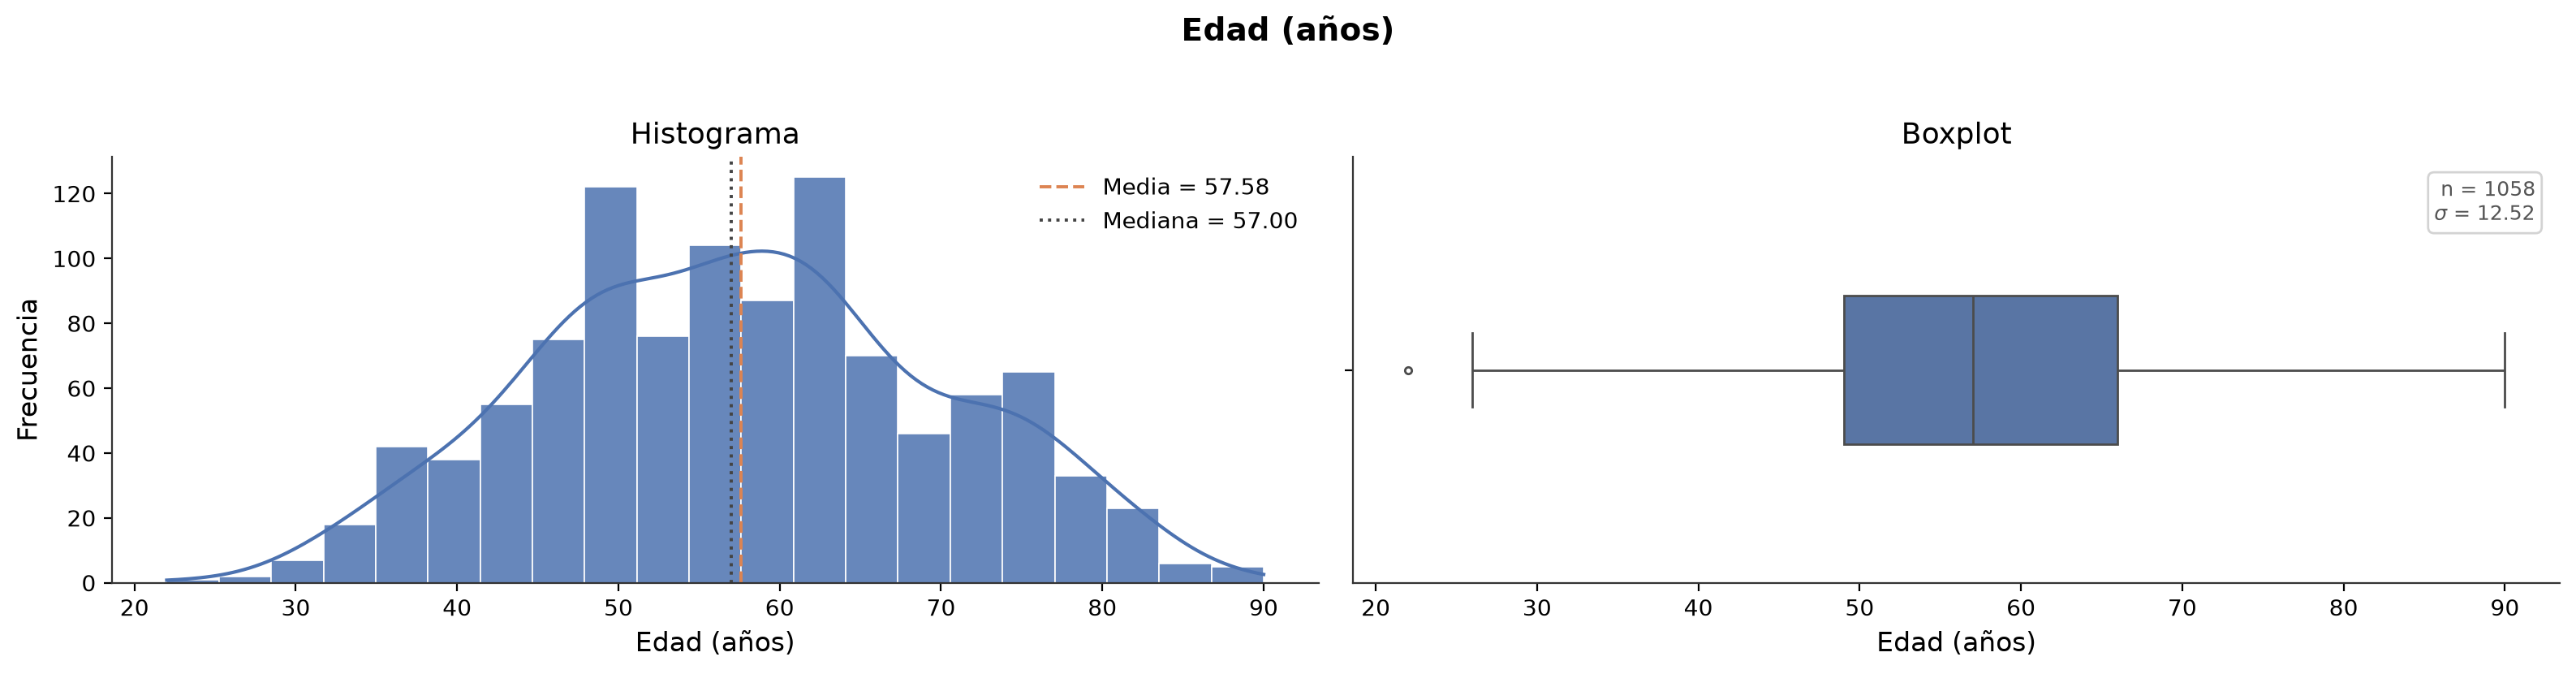
\includegraphics[width=0.75\textwidth]{images/fig41-bcnb-age.png}
\caption{Distribución de la variable \textit{Age} en BCNB (datos originales).}
\label{fig:bcnb-age}
\end{figure}

\begin{figure}[htbp]
\centering
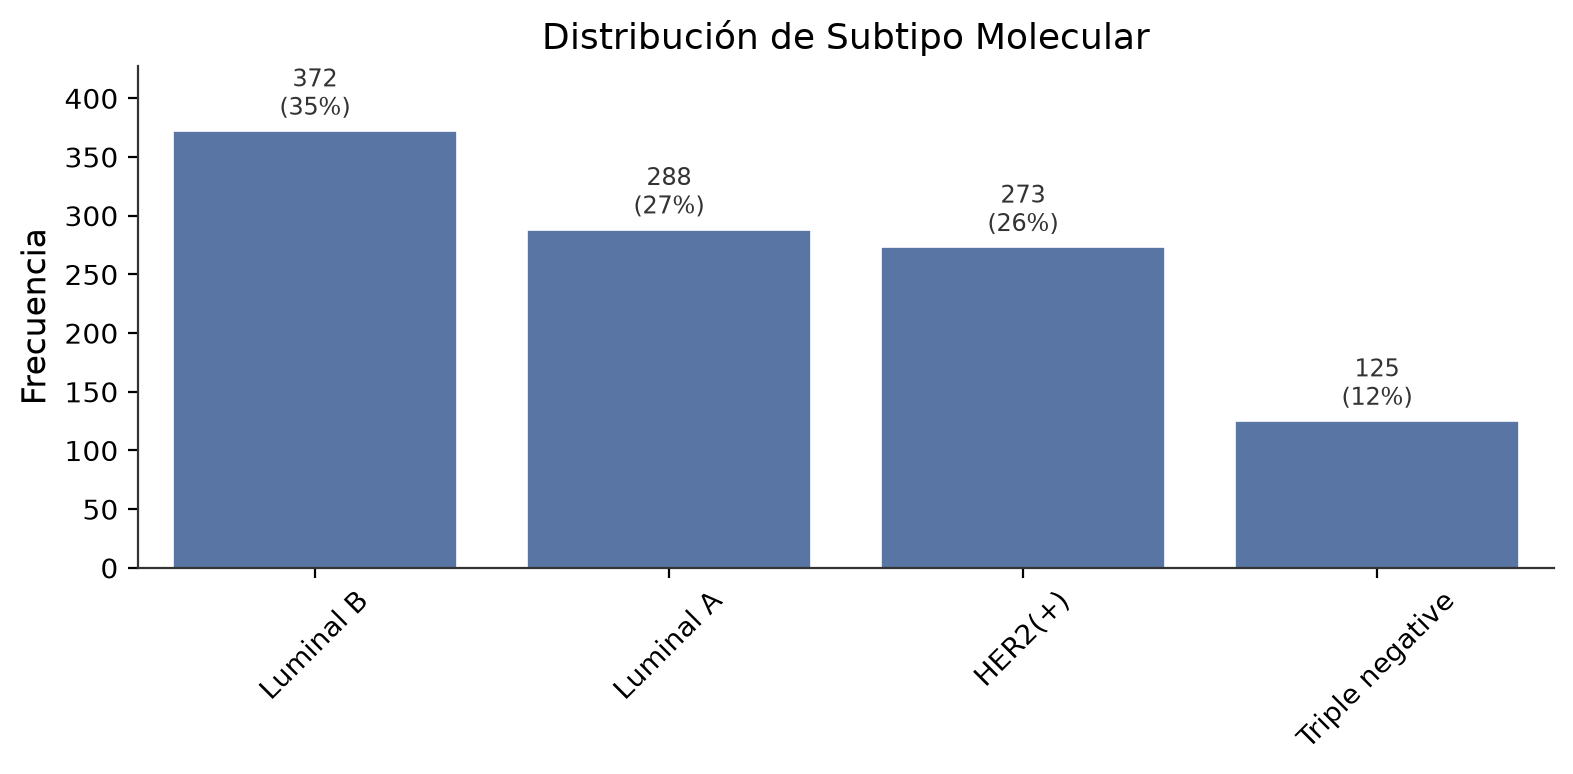
\includegraphics[width=0.75\textwidth]{images/fig43-bcnb-molecular-subtype.png}
\caption{Distribución de la variable \textit{Molecular subtype} en BCNB (datos originales).}
\label{fig:bcnb-molecular-subtype}
\end{figure}

% \section{Visualizaciones post-curación}
% \label{appendix:visualizaciones_postcuracion}

% Esta sección presenta las visualizaciones de las distribuciones post-curación referenciadas en la Sección~\ref{sec:visualizacion_distribuciones} del Capítulo~\ref{cap:caracterizacion_datasets}. Las Figuras~\ref{fig:surgen-site-total-curated}~y~\ref{fig:surgen-side-total-curated} presentan la distribución agregada del sitio tumoral y la lateralidad en SurGen (SR386 y SR1482 combinados), tras el proceso de armonización descrito en la Sección~\ref{sec:caracterizacion_datasets}.

% \begin{figure}[htbp]
% \centering
% 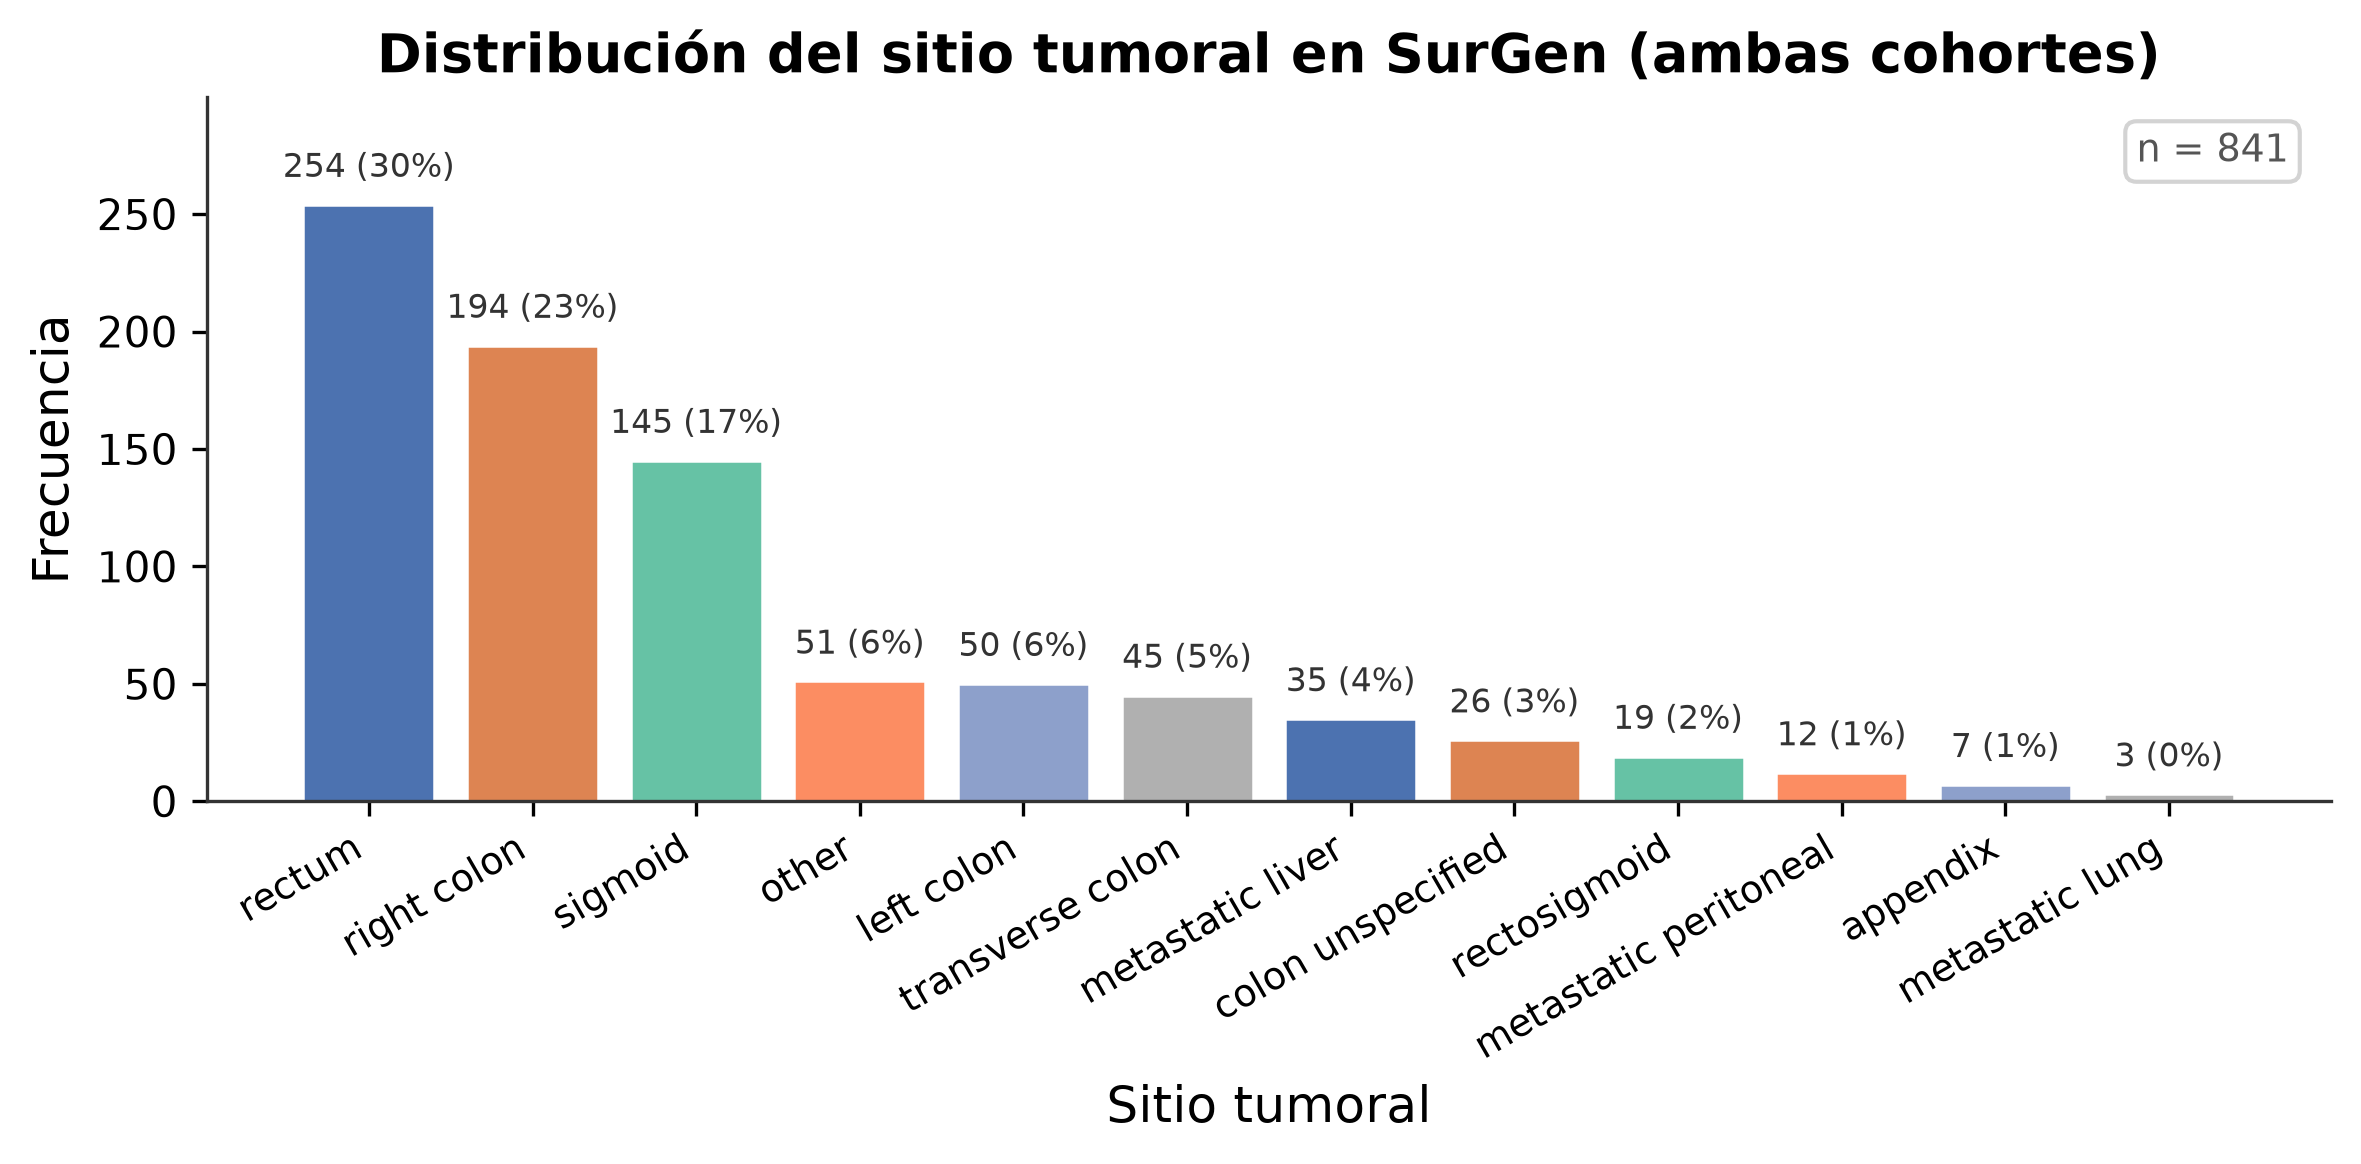
\includegraphics[width=0.8\textwidth]{images/fig47-surgen-site-total-curated.png}
% \caption{Distribución agregada del sitio tumoral en SurGen (SR386~+~SR1482 combinados, post-curación).}
% \label{fig:surgen-site-total-curated}
% \end{figure}

% \begin{figure}[htbp]
% \centering
% 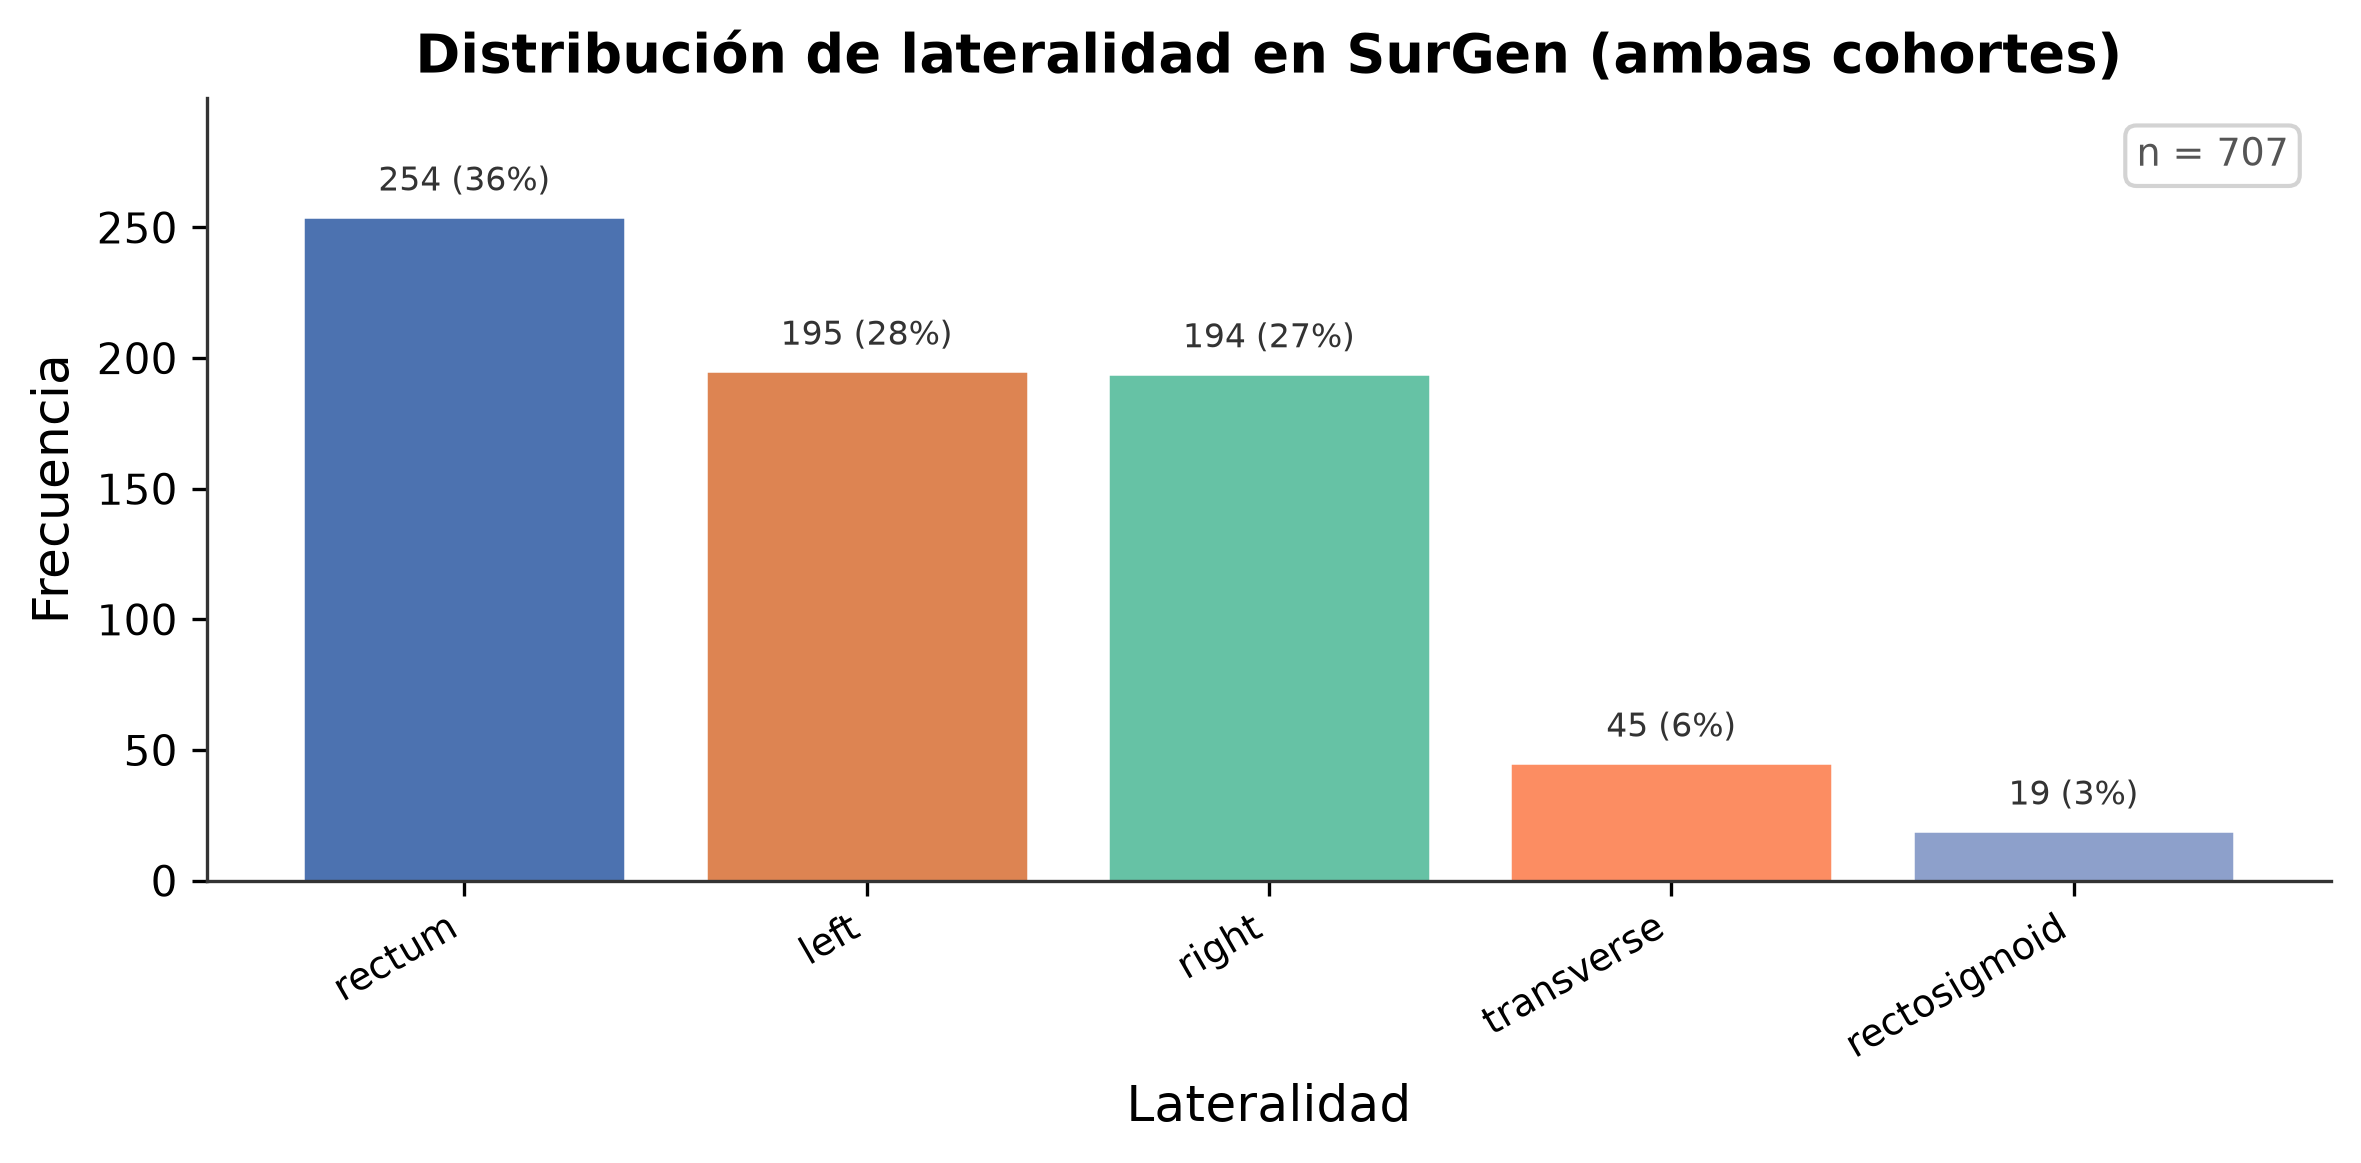
\includegraphics[width=0.8\textwidth]{images/fig48-surgen-side-total-curated.png}
% \caption{Distribución agregada de lateralidad en SurGen (SR386~+~SR1482 combinados, post-curación). La lateralidad se deriva del sitio tumoral y permite una comparación más compacta entre cohortes.}
% \label{fig:surgen-side-total-curated}
% \end{figure}


\section{Extracción de variables clínicas desde texto libre en HISTAI}
\label{appendix:extraccion_histai}

Los metadatos clínicos de HISTAI se encuentran mayormente en campos de texto libre dentro del informe histopatológico. Para recuperar variables comparables con los demás conjuntos de datos, se implementó un pipeline de extracción basado en expresiones regulares y recodificación explícita, ejecutado sobre un campo de texto unificado por caso. Esta sección documenta las fuentes textuales utilizadas, los patrones aplicados por variable, los criterios de resolución de conflictos, el tratamiento de los casos no parseables, la cobertura resultante y las limitaciones del proceso, incluyendo la ausencia de una validación manual con muestra independiente.

\subsection{Fuentes textuales y composición del texto analizado}

Para cada subcohorte se concatenaron los campos narrativos disponibles en el orden indicado (Tabla~\ref{tab:anexo_campos_histai}), generando el campo \texttt{full\_text} sobre el cual se ejecutaron todas las reglas. El orden de concatenación es relevante porque, salvo indicación contraria, las reglas recuperan la \emph{primera} coincidencia en el texto resultante: los campos que aparecen primero adquieren prioridad de facto.

\begin{table}[htbp]
\centering
\caption{Campos narrativos considerados en la extracción por subcohorte HISTAI.}
\label{tab:anexo_campos_histai}
\small
\begin{tabular}{lccl}
\toprule
Subcohorte & N & Campos concatenados (en orden) \\
\midrule
HISTAI-Breast & 1489 & diagnosis, conclusion, additional\_info, micro\_protocol  \\
HISTAI-CRC-B1 & 878 & diagnosis, conclusion, grossing, micro\_protocol, additional\_info  \\
HISTAI-CRC-B2 & 57 & diagnosis, conclusion, grossing, micro\_protocol, additional\_info  \\
\bottomrule
\end{tabular}
\end{table}

Además, la etapa de mapeo semántico previa (descrita en la Sección~\ref{appendix:detalles_datasetanalyzer}) generó, a partir del campo \texttt{diagnosis}, las variables derivadas de diagnóstico (grupo taxonómico y sitio/lateralidad taxonómicos), que sirven de base para la clasificación de sitio y lateralidad del dominio colorrectal.

\subsection{Reglas de extracción en el dominio de mama}

La Tabla~\ref{tab:anexo_reglas_mama} resume los patrones aplicados sobre \texttt{full\_text} en HISTAI-Breast y su recodificación. Las menciones se realizan sobre texto en minúsculas; en ER/PR la búsqueda está acotada a la oración (el patrón considera texto hasta el primer punto), mientras en HER2 y Ki-67 la búsqueda es global al documento.

\begin{table}[htbp]
\centering
\caption{Reglas de extracción por biomarcador en HISTAI-Breast.}
\label{tab:anexo_reglas_mama}
\footnotesize
\setlength{\tabcolsep}{3pt}
\resizebox{\textwidth}{!}{%
\begin{tabular}{p{1.6cm}p{4.6cm}p{6.2cm}p{3.4cm}}
\toprule
Variable & Patrón aplicado & Lectura y recodificación & Ejemplo (abreviado) \\
\midrule
ER & \texttt{\textbackslash{}ber\textbackslash{}b[.\^{}]*negative} primero; si no, \texttt{\textbackslash{}ber\textbackslash{}b[.\^{}]*positive} & \emph{negative} $\rightarrow$ 0 (negativo); \emph{positive} $\rightarrow$ 1 (positivo); si ninguno en la oración, sin dato & ``\ldots ER: positive (more than 10\% of tumor cells) \ldots'' $\rightarrow$ 1 \\
PR & \texttt{\textbackslash{}bpr\textbackslash{}b[.\^{}]*negative} primero; si no, \texttt{\textbackslash{}bpr\textbackslash{}b[.\^{}]*positive} & idem ER & ``\ldots PR: positive \ldots'' $\rightarrow$ 1 \\
HER2 & \texttt{her2[.\^{}0-9]*([0-3])\textbackslash{}s*+?} & score 0 o 1 $\rightarrow$ 0 (negativo/bajo); 2 $\rightarrow$ 1 (equívoco); 3 $\rightarrow$ 2 (positivo) & ``\ldots anti-Her2 (c-erbB-2) antibody --- 3 points: strong complete membrane staining \ldots'' $\rightarrow$ 2 \\
HER2 (fallback) & si sin score: \texttt{her2} y \texttt{negative} en el documento; luego \texttt{her2} y (\texttt{undetermined} o \texttt{equivocal}) & \emph{negative} $\rightarrow$ 0; \emph{undetermined}/\emph{equivocal} $\rightarrow$ 1 (equívoco) & ``\ldots HER2 status undetermined \ldots'' $\rightarrow$ 1 \\
Ki-67 & \texttt{ki-?67[.\^{}0-9]*([0-9]+(?:\textbackslash{}.[0-9]+)?)} & primer número tras la mención; categorías: $<10$ baja, $10$--$20$ intermedia, $>20$ alta & ``\ldots Ki-67 proliferation index: 30\% \ldots'' $\rightarrow$ 30 (alta) \\
Subtipo & menciones directas en el orden: \texttt{triple negative}; \texttt{luminal a}; \texttt{luminal b}; \texttt{her2} + (\texttt{positive} o \texttt{3+}) & Triple negative; Luminal A; Luminal B; HER2+; sin derivación desde biomarcadores & ``\ldots Surrogate molecular subtype: Luminal A \ldots'' $\rightarrow$ Luminal A \\
\bottomrule
\end{tabular}%
}
\end{table}

Nota: la codificación de subtipo se basa exclusivamente en la mención explícita del subtipo en el informe; no se deriva de los biomarcadores extraídos. Como referencia de armonización, en BCNB los valores estructurados se recodificaron con la misma escala (ER/PR binarios; HER2 0/0+ y 1/1+ $\rightarrow$ 0, 2/2+ $\rightarrow$ 1, 3/3+ $\rightarrow$ 2; Ki-67 con rango promediado: \texttt{"15-20"} $\rightarrow$ 15) y en HSI-BC los códigos \texttt{0/1/2} se interpretaron como negativo/positivo/equívoco (HER2) y el código de Ki-67 se convirtió a porcentaje mediante una correspondencia heurística \texttt{\{0,1,2,3,4\}$\rightarrow$\{5,10,20,30,40\}}.

\subsection{Reglas de extracción en el dominio colorrectal}

\paragraph{Sitio anatómico.} La detección se realiza en dos pasos. Primero, sobre el diagnóstico normalizado (con expansión de códigos ICD-10 como C18.\textit{x}, C19, C20, D12.5 y D37.7), se aplica una lista ordenada de 11 reglas de sitio (rectosigmoide, recto, sigmoide, colon descendente, flexura esplénica, colon transverso, flexura hepática, colon ascendente, ciego, canal anal y colon inespecífico), devolviendo el primer patrón que coincide; si ninguno, la etiqueta \texttt{unspecified}. Segundo, las etiquetas resultantes se agrupan en el vocabulario de tarea de nueve clases que comparten HISTAI-CRC-B1, HISTAI-CRC-B2 y SurGen:

\begin{center}
\small
\texttt{\{rectum, sigmoid, right\_colon, left\_colon, transverse\_colon, rectosigmoid, colon\_unspecified, metastatic\_liver, other\}}
\end{center}

La categoría \emph{Otros} (\texttt{other}) queda definida por la regla de caída (sin coincidencia de ningún patrón). En HISTAI-CRC-B1 su composición observada es: diagnósticos sin mención de sitio (117 casos), flexura esplénica (11) y canal anal (2); en SurGen, la clase colapsa además las localizaciones de baja frecuencia declaradas en la Sección~\ref{sec:caracterizacion_datasets} (apéndice, metástasis peritoneales y pulmonares; n=12, 7 y 3, respectivamente). Cabe señalar una limitación del mapeo: al aplicarse sobre la etiqueta taxonómica normalizada (con guiones bajos) y no sobre el texto original, el literal \texttt{hepatic flexure} (con espacio) no activa la regla de colon derecho, y la subcadena \texttt{hepatic} activa la regla de metástasis hepática; por ello, 18 casos de flexura hepática del colon (C18.3) quedaron codificados como \texttt{metastatic\_liver} en HISTAI-CRC-B1. El impacto de esta decisión se limita a la composición de la clase \texttt{metastatic\_liver} (en la Tabla~\ref{tab:resumen_frecuencias_colorrectal}, 18 casos, 2,1\,\%).

\paragraph{Lateralidad.} Derivada del sitio agrupado: colon derecho $\rightarrow$ \texttt{right}; colon izquierdo y sigmoide $\rightarrow$ \texttt{left}; transverso $\rightarrow$ \texttt{transverse}; recto $\rightarrow$ \texttt{rectum}; rectosigmoide $\rightarrow$ \texttt{rectosigmoid}; el resto (colon inespecífico, \emph{Otros} y metástasis hepática) queda sin dato.

\paragraph{Estadificación y variables histopatológicas.} Sobre \texttt{full\_text} se extraen, con el mismo criterio de primera coincidencia: grado (G1--G3 por \texttt{g1}/\texttt{grade: 1}/\texttt{1-high grade differentiation} y equivalentes verbales \emph{well/moderately/poorly differentiated}); etapa patológica por patrones \texttt{pt([0-4][ab]?)}, \texttt{pn([0-2][abc]?)} y \texttt{pm([01][abcx]?)} (con variante clínica \texttt{cm1} $\rightarrow$ cM1); ganglios examinados y positivos mediante \texttt{total number:}, \texttt{number examined:}, \texttt{number of involved/affected lymph nodes:} y la notación \texttt{n\textit{X}(\textit{p}/\textit{e})}; estado ganglionar derivado del conteo de positivos (0 $\rightarrow$ N0; 1--3 $\rightarrow$ N+(1--3); $>$3 $\rightarrow$ N+(>3); en ausencia de conteo, desde pN); estadio simplificado derivado (M1 $\rightarrow$ IV; N1/N2 $\rightarrow$ III; T3/T4 $\rightarrow$ II; T1/T2 $\rightarrow$ I); e invasión linfovascular y perineural por patrones de presencia/ausencia explícitos. Estas variables se generaron para caracterización descriptiva y comparabilidad con SurGen, pero no fueron seleccionadas como tareas de clasificación en el Capítulo~\ref{cap:seleccion_modelos}. Los biomarcadores moleculares (MMR/MSI, KRAS/NRAS/BRAF) no fueron extraídos desde el texto en las subcohortes HISTAI, quedando como datos faltantes por estructura.

\subsection{Resolución de conflictos}

La política general es \emph{primera coincidencia sobre el texto concatenado}, lo que equivale a priorizar, en mama, \texttt{conclusion} sobre \texttt{additional\_info} sobre \texttt{micro\_protocol}, y en CRC, \texttt{diagnosis} sobre \texttt{conclusion} sobre \texttt{grossing} sobre \texttt{micro\_protocol} sobre \texttt{additional\_info}. Con ello, si un mismo marcador aparece con valores distintos en dos campos (por ejemplo, ``HER2: 2+'' en la conclusión y ``HER2: 3+'' en el protocolo microscópico), prevalece la primera mención. Las excepciones son: (i) ER y PR evalúan la mención negativa antes que la positiva dentro de la oración (ante ambas menciones en la misma oración prevalece \emph{negative}); (ii) en HER2, el score numérico prevalece sobre los fallbacks textuales; y (iii) en subtipo, el orden de evaluación de los patrones (\texttt{triple negative} antes que \texttt{luminal a} antes que \texttt{luminal b} antes que \texttt{her2+}) define la jerarquía.

\subsection{Cobertura resultante}

La Tabla~\ref{tab:anexo_cobertura_mama} reporta la cobertura por marcador en HISTAI-Breast (denominador: cohorte curada, N=1489). La pérdida se concentra en informes sin panel de inmunohistoquímica o sin mención explícita del marcador, no en fallas de parsing de menciones presentes.

\begin{table}[htbp]
\centering
\caption{Cobertura y distribución de clases por marcador en HISTAI-Breast tras la extracción textual.}
\label{tab:anexo_cobertura_mama}
\footnotesize
\setlength{\tabcolsep}{3pt}
\resizebox{\textwidth}{!}{%
\begin{tabular}{lcccl}
\toprule
Marcador & N con dato & Cobertura (\%) & Distribución de clases (n; \%) \\
\midrule
ER & 855 & 57,4 & Negativo 313 (36,6); Positivo 542 (63,4) \\
PR & 849 & 57,0 & Negativo 366 (43,1); Positivo 483 (56,9) \\
HER2 & 878 & 59,0 & Negativo/bajo 133 (15,1); Equívoco 554 (63,1); Positivo 191 (21,8) \\
Ki-67 (numérico) & 889 & 59,7 & Categorías $<10$ / $10$--$20$ / $>20$ \\
Subtipo molecular & 852 & 57,2 & Luminal A 143 (16,8); Luminal B 353 (41,4); HER2+ 281 (33,0); Triple negativo 75 (8,8) \\
\bottomrule
\end{tabular}%
}
\end{table}

En colorrectal, el sitio anatómico se extrae en el 100\,\% de los casos (la regla de caída siempre asigna una categoría), mientras la lateralidad queda sin dato en HISTAI-CRC-B1 para 263 casos (colon inespecífico 115, \emph{Otros} 130, metástasis hepática 18), resultando en una cobertura de 70,0\,\%; en HISTAI-CRC-B2 la cobertura es de 80,7\,\% (Tabla~\ref{tab:trazabilidad_colorrectal}).

	\chapter{Criterios de Asignación de Indicadores de Preselección}
\label{appendix:criterios_preseleccion}

En este apéndice se documentan los criterios utilizados para asignar los niveles cualitativos (bajo, medio, alto) a cada indicador de la Tabla~\ref{tab:indicadores_preseleccion} del Capítulo~\ref{cap:caracterizacion_datasets}. Su propósito es garantizar la reproducibilidad de la evaluación y explicitar los umbrales aplicados.

La clasificación de \textbf{Escala} se basa en el número de registros de la cohorte \textit{raw}. La \textbf{Completitud} se evalúa mediante el porcentaje global de celdas pobladas en los metadatos, complementado con el nivel de \textit{missingness} de variables clave cuando el valor global resulta limítrofe. La \textbf{Cobertura} considera la disponibilidad de variables demográficas y clínicas relevantes para el análisis de \textit{bias}. La \textbf{Compatibilidad} evalúa la existencia de otros conjuntos de datos del mismo dominio clínico con variables comparables.

\begin{table}[htbp]
\centering
\caption{Criterios de asignación de niveles por indicador de preselección.}
\label{tab:criterios_preseleccion}
\small
\setlength{\tabcolsep}{5pt}
\begin{tabular}{p{2.5cm} p{3.8cm} p{3.8cm} p{3.8cm}}
\toprule
\textbf{Indicador} & \textbf{Bajo} & \textbf{Medio} & \textbf{Alto} \\
\midrule

\textbf{Escala} &
$\geq$1500 registros &
100--1499 registros &
$<$100 registros \\
& (\textit{Grande}) & (\textit{Mediana}) & (\textit{Pequeña}) \\
\addlinespace

\textbf{Completitud} &
$\geq$90\% de celdas pobladas &
75--89\% de celdas pobladas &
$<$75\% de celdas pobladas \\
& Se considera \textit{Completa} cuando alcanza el 100\%. &
Si variables clave presentan $>$50\% de valores faltantes, la clasificación se degrada un nivel. &
\\
\addlinespace

\textbf{Cobertura} &
Dispone de edad, sexo y al menos un biomarcador relevante (HER2, subtipo molecular, estado mutacional). &
Dispone de edad y sexo, más variables clínicas básicas sin biomarcadores moleculares. &
Solo dispone de variables demográficas básicas sin biomarcadores ni variables clínicas específicas del dominio. \\
\addlinespace

\textbf{Compatibilidad} &
Existen al menos dos conjuntos de datos del mismo dominio clínico con variables comparables y armonizables. &
Existe un conjunto de datos del mismo dominio, pero la comparabilidad es parcial o requiere armonización adicional. &
No existe repetición del dominio clínico en otros conjuntos de datos de la revisión. \\
\bottomrule
\end{tabular}
\end{table}

La verificación de estos criterios contra los valores numéricos de cada conjunto de datos se realizó a partir de las tablas de caracterización global (Tabla~\ref{tab:dataset_global_summary} del Capítulo~\ref{cap:caracterizacion_datasets}) y de síntesis de recursos (Tabla~\ref{tab:resumen_datasets_global} del Apéndice~\ref{appendix:tablasdatasets}).

\begin{table}[htbp]
\centering
\caption{Verificación de la asignación de niveles para cada conjunto de datos.}
\label{tab:verificacion_preseleccion}
\small
\setlength{\tabcolsep}{4pt}
\begin{tabular}{lcccc}
\toprule
\textbf{Dataset} & \textbf{n} & \textbf{Completitud (\%)} & \textbf{Cobertura vars.} & \textbf{Compatibilidad} \\
\midrule
Ovarian          & 78   & 91,9  & Demográficas + clínicas bás.       & Ninguna \\
BCNB             & 1058 & 99,0  & Edad, sexo, HER2, subtipo mol.     & Mama (HSI-BC, HISTAI-Br) \\
CLWD             & 408  & 100   & Demográficas + clínicas bás.       & Ninguna \\
NDB-UFES         & 237  & 95,5  & Edad, sexo, etnia                  & Ninguna \\
TDBTA            & 3115 & 71,2  & Edad, sexo, diagnóstico, grado     & Ninguna \\
SurGen           & 843 & 53,4  & Edad, sexo, sitio, biomarcadores   & Colorrectal (HISTAI-CRC) \\
HSI-BC          & 47   & 99,3  & Edad, sexo, etnia, HER2, subtipo   & Mama (BCNB, HISTAI-Br) \\
SOPHIE           & 61   & 70,3  & Edad, sexo, diagnóstico            & Ninguna \\
HISTAI-Breast    & 1489 & 85,3  & Edad, sexo, HER2, subtipo mol.     & Mama (BCNB, HSI-BC) \\
HISTAI-CRC-B1    & 878  & 82,9  & Edad, sexo, sitio anatómico        & Colorrectal (SurGen) \\
HISTAI-CRC-B2    & 57   & 98,2  & Edad, sexo, sitio anatómico        & Colorrectal (SurGen) \\
\bottomrule
\end{tabular}
\end{table}

	\chapter{Atributos técnicos de los modelos fundacionales seleccionados}
\label{apx:atributos_modelos}

\begin{table}[htbp]
\centering
\caption{Atributos relevantes de los modelos fundacionales seleccionados.}
\label{tab:atributos_modelos}
\small
\begin{tabularx}{\textwidth}{>{\raggedright\arraybackslash}p{2.2cm} >{\raggedright\arraybackslash}X >{\raggedright\arraybackslash}X >{\raggedright\arraybackslash}X >{\raggedright\arraybackslash}X}
\toprule
\textbf{Atributo} & \textbf{Phikon-v2} & \textbf{UNI2-h} & \textbf{Prov-GigaPath} & \textbf{Virchow2} \\
\midrule
Tipo de modelo & Encoder visual fundacional & Encoder visual fundacional & Encoder de parche + agregador de slide (LongNet) & Encoder visual fundacional \\
Arquitectura base & ViT-L/16 & ViT-H/14 & ViT-g/14 (parche) + LongNetViT (slide) & ViT-H/14 \\
Parámetros & $\sim$0.3B & $\sim$0.68B & $\sim$1.1B (parche) & $\sim$0.63B \\
Estrategia de preentrenamiento & Auto-supervisado, DINOv2 (DINO+iBOT+KoLeo) & Auto-supervisado, DINOv2 & DINOv2 (parche) + MAE con LongNet (slide) & Auto-supervisado, DINOv2 multiescala \\
Escala de datos de preentrenamiento & 456M parches / $>$58k WSI (TCGA, CPTAC, GTEx) & 200M+ parches / 350k+ WSI institucionales & 1.3B parches / 171k WSI institucionales & 3.1M WSI H\&E + 400k IHC \\
Unidad de entrada & Parche & Parche & Parche\textsuperscript{1} & Parche \\
Dimensión del embedding & 1024 & 1536 & 1536 (encoder de parche) & 2560 \\
Acceso & Público (CC-BY-NC 4.0) & Restringido (AP\textsuperscript{2}) & Público (CC-BY-NC 4.0) & Restringido (AP\textsuperscript{2})\\
Transparencia de datos de preentrenamiento & Parcial; datos públicos reportados & Parcial; procedencia agregada, datos institucionales privados & Parcial; datos institucionales privados & Parcial; datos institucionales privados \\
\bottomrule
\end{tabularx}
\begin{flushleft}
\footnotesize{\textsuperscript{1}Se utiliza únicamente el encoder de parche de Prov-GigaPath como extractor de representaciones; el agregador de slide basado en LongNet no se emplea en esta tesis.}
\footnotesize{\textsuperscript{2}AP: Aprobación Institucional.}
\end{flushleft}
\end{table}

	\chapter{Resultados completos de la evaluación de modelos fundacionales}
\label{anexo:resultados_completos}

\section{Utilidad global}
\label{anexo:utilidad_global}

\subsection{T1 -- HER2}

\begin{table}[H]
\centering
\caption{Utilidad global por modelo, tarea T1-HER2. IC 95\% obtenido por bootstrap (1000 remuestreos, a nivel de paciente).}
\label{tab:anexo_her2_utilidad}
\resizebox{\textwidth}{!}{%
\begin{tabular}{l l c c c c c c}
\toprule
\textbf{Dataset} & \textbf{Modelo} & \textbf{n\_test} & \textbf{BA} & \textbf{IC95\% BA} & \textbf{Macro-F1} & \textbf{IC95\% F1} & \textbf{AUC (OVR macro)} \\
\midrule
BCNB & UNI2 & 1058 & 0.455 & [0.424, 0.487] & 0.457 & [0.426, 0.489] & 0.632 \\
BCNB & Virchow2 & 1058 & 0.434 & [0.404, 0.465] & 0.434 & [0.404, 0.466] & 0.620 \\
BCNB & Phikon-v2 & 1058 & 0.418 & [0.387, 0.449] & 0.415 & [0.384, 0.446] & 0.602 \\
BCNB & Prov-GigaPath & 1058 & 0.447 & [0.418, 0.477] & 0.445 & [0.415, 0.475] & 0.624 \\
HISTAI-Breast & UNI2 & 870 & 0.364 & [0.335, 0.394] & 0.365 & [0.332, 0.398] & 0.548 \\
HISTAI-Breast & Virchow2 & 870 & 0.366 & [0.335, 0.398] & 0.368 & [0.333, 0.402] & 0.543 \\
HISTAI-Breast & Phikon-v2 & 870 & 0.381 & [0.349, 0.414] & 0.384 & [0.349, 0.419] & 0.548 \\
HISTAI-Breast & Prov-GigaPath & 870 & 0.377 & [0.347, 0.410] & 0.378 & [0.345, 0.414] & 0.546 \\
HSI-BC & UNI2 & 44 & 0.438 & [0.318, 0.594] & 0.441 & [0.333, 0.581] & 0.389 \\
HSI-BC & Virchow2 & 44 & 0.417 & [0.353, 0.472] & 0.405 & [0.353, 0.450] & 0.483 \\
HSI-BC & Phikon-v2 & 44 & 0.278 & [0.194, 0.361] & 0.312 & [0.241, 0.380] & 0.184 \\
HSI-BC & Prov-GigaPath & 44 & 0.562 & [0.359, 0.762] & 0.547 & [0.382, 0.714] & 0.597 \\
\bottomrule
\end{tabular}
}
\end{table}

\begin{table}[H]
\centering
\caption{Sensibilidad (recall) por clase, tarea T1-HER2, dataset BCNB ($K=3$). Clases en filas y un modelo por columna; las clases ausentes en la cohorte se marcan con ``--''.}
\label{tab:anexo_her2_sensibilidad}
\begin{tabular}{l c c c c}
\toprule
\textbf{Clase} & \textbf{UNI2} & \textbf{Virchow2} & \textbf{Phikon-v2} & \textbf{Prov-GigaPath} \\
\midrule
\textbf{n\_test} & 1058 & 1058 & 1058 & 1058 \\
0/1+ & 0.360 & 0.358 & 0.325 & 0.331 \\
2+ & 0.625 & 0.590 & 0.573 & 0.607 \\
3+ & 0.379 & 0.354 & 0.354 & 0.403 \\
\bottomrule
\end{tabular}
\end{table}

\begin{table}[H]
\centering
\caption{Sensibilidad (recall) por clase, tarea T1-HER2, dataset HISTAI-Breast ($K=3$). Clases en filas y un modelo por columna; las clases ausentes en la cohorte se marcan con ``--''.}
\label{tab:anexo_her2_sensibilidad_histai}
\begin{tabular}{l c c c c}
\toprule
\textbf{Clase} & \textbf{UNI2} & \textbf{Virchow2} & \textbf{Phikon-v2} & \textbf{Prov-GigaPath} \\
\midrule
\textbf{n\_test} & 870 & 870 & 870 & 870 \\
0/1+ & 0.171 & 0.186 & 0.194 & 0.140 \\
2+ & 0.747 & 0.709 & 0.715 & 0.745 \\
3+ & 0.173 & 0.204 & 0.236 & 0.246 \\
\bottomrule
\end{tabular}
\end{table}

\begin{table}[H]
\centering
\caption{Sensibilidad (recall) por clase, tarea T1-HER2, dataset HSI-BC ($K=3$). Clases en filas y un modelo por columna; las clases ausentes en la cohorte se marcan con ``--''.}
\label{tab:anexo_her2_sensibilidad_hsibc}
\begin{tabular}{l c c c c}
\toprule
\textbf{Clase} & \textbf{UNI2} & \textbf{Virchow2} & \textbf{Phikon-v2} & \textbf{Prov-GigaPath} \\
\midrule
\textbf{n\_test} & 44 & 44 & 44 & 44 \\
0/1+ & 0.750 & 0.833 & 0.556 & 0.750 \\
2+ & -- & -- & -- & -- \\
3+ & 0.125 & 0.000 & 0.000 & 0.375 \\
\bottomrule
\end{tabular}
\end{table}

\subsection{T2 -- Subtipo molecular}

\begin{table}[H]
\centering
\caption{Utilidad global por modelo, tarea T2-MolSub. IC 95\% obtenido por bootstrap (1000 remuestreos, a nivel de paciente).}
\label{tab:anexo_molsub_utilidad}
\resizebox{\textwidth}{!}{%
\begin{tabular}{l l c c c c c c}
\toprule
\textbf{Dataset} & \textbf{Modelo} & \textbf{n\_test} & \textbf{BA} & \textbf{IC95\% BA} & \textbf{Macro-F1} & \textbf{IC95\% F1} & \textbf{AUC (OVR macro)} \\
\midrule
BCNB & UNI2 & 1058 & 0.482 & [0.450, 0.514] & 0.479 & [0.445, 0.510] & 0.740 \\
BCNB & Virchow2 & 1058 & 0.427 & [0.396, 0.458] & 0.422 & [0.392, 0.451] & 0.706 \\
BCNB & Phikon-v2 & 1058 & 0.434 & [0.403, 0.466] & 0.429 & [0.398, 0.461] & 0.697 \\
BCNB & Prov-GigaPath & 1058 & 0.472 & [0.441, 0.506] & 0.470 & [0.438, 0.504] & 0.727 \\
HISTAI-Breast & UNI2 & 842 & 0.361 & [0.326, 0.398] & 0.361 & [0.325, 0.398] & 0.626 \\
HISTAI-Breast & Virchow2 & 842 & 0.354 & [0.320, 0.390] & 0.351 & [0.316, 0.386] & 0.622 \\
HISTAI-Breast & Phikon-v2 & 842 & 0.327 & [0.291, 0.363] & 0.327 & [0.289, 0.360] & 0.607 \\
HISTAI-Breast & Prov-GigaPath & 842 & 0.341 & [0.309, 0.378] & 0.341 & [0.308, 0.379] & 0.619 \\
HSI-BC & UNI2 & 44 & 0.317 & [0.216, 0.445] & 0.307 & [0.208, 0.390] & 0.595 \\
HSI-BC & Virchow2 & 44 & 0.172 & [0.098, 0.274] & 0.171 & [0.105, 0.244] & 0.473 \\
HSI-BC & Phikon-v2 & 44 & 0.217 & [0.133, 0.319] & 0.210 & [0.139, 0.281] & 0.473 \\
HSI-BC & Prov-GigaPath & 44 & 0.334 & [0.202, 0.506] & 0.317 & [0.205, 0.449] & 0.616 \\
\bottomrule
\end{tabular}
}
\end{table}

\begin{table}[H]
\centering
\caption{Sensibilidad (recall) por clase, tarea T2-MolSub, dataset BCNB ($K=4$). Clases en filas y un modelo por columna; las clases ausentes en la cohorte se marcan con ``--''.}
\label{tab:anexo_molsub_sensibilidad}
\begin{tabular}{l c c c c}
\toprule
\textbf{Clase} & \textbf{UNI2} & \textbf{Virchow2} & \textbf{Phikon-v2} & \textbf{Prov-GigaPath} \\
\midrule
\textbf{n\_test} & 1058 & 1058 & 1058 & 1058 \\
Luminal A & 0.403 & 0.365 & 0.351 & 0.403 \\
Luminal B & 0.559 & 0.492 & 0.503 & 0.543 \\
HER2+ & 0.399 & 0.403 & 0.363 & 0.388 \\
Triple Negative & 0.568 & 0.448 & 0.520 & 0.552 \\
\bottomrule
\end{tabular}
\end{table}

\begin{table}[H]
\centering
\caption{Sensibilidad (recall) por clase, tarea T2-MolSub, dataset HISTAI-Breast ($K=4$). Clases en filas y un modelo por columna; las clases ausentes en la cohorte se marcan con ``--''.}
\label{tab:anexo_molsub_sensibilidad_histai}
\begin{tabular}{l c c c c}
\toprule
\textbf{Clase} & \textbf{UNI2} & \textbf{Virchow2} & \textbf{Phikon-v2} & \textbf{Prov-GigaPath} \\
\midrule
\textbf{n\_test} & 842 & 842 & 842 & 842 \\
Luminal A & 0.315 & 0.329 & 0.259 & 0.273 \\
Luminal B & 0.617 & 0.597 & 0.540 & 0.591 \\
HER2+ & 0.284 & 0.262 & 0.280 & 0.284 \\
Triple Negative & 0.230 & 0.230 & 0.230 & 0.216 \\
\bottomrule
\end{tabular}
\end{table}

\begin{table}[H]
\centering
\caption{Sensibilidad (recall) por clase, tarea T2-MolSub, dataset HSI-BC ($K=4$). Clases en filas y un modelo por columna; las clases ausentes en la cohorte se marcan con ``--''.}
\label{tab:anexo_molsub_sensibilidad_hsibc}
\begin{tabular}{l c c c c}
\toprule
\textbf{Clase} & \textbf{UNI2} & \textbf{Virchow2} & \textbf{Phikon-v2} & \textbf{Prov-GigaPath} \\
\midrule
\textbf{n\_test} & 44 & 44 & 44 & 44 \\
Luminal A & 0.556 & 0.222 & 0.333 & 0.444 \\
Luminal B & 0.714 & 0.464 & 0.536 & 0.643 \\
HER2+ & 0.000 & 0.000 & 0.000 & 0.000 \\
Triple Negative & 0.000 & 0.000 & 0.000 & 0.250 \\
\bottomrule
\end{tabular}
\end{table}

\subsection{T3 -- Sitio anatómico}

\begin{table}[H]
\centering
\caption{Utilidad global por modelo, tarea T3-Site. IC 95\% obtenido por bootstrap (1000 remuestreos, a nivel de paciente).}
\label{tab:anexo_site_utilidad}
\resizebox{\textwidth}{!}{%
\begin{tabular}{l l c c c c c c}
\toprule
\textbf{Dataset} & \textbf{Modelo} & \textbf{n\_test} & \textbf{BA} & \textbf{IC95\% BA} & \textbf{Macro-F1} & \textbf{IC95\% F1} & \textbf{AUC (OVR macro)} \\
\midrule
HISTAI-CRC-B1 & UNI2 & 878 & 0.203 & [0.180, 0.227] & 0.204 & [0.181, 0.226] & 0.598 \\
HISTAI-CRC-B1 & Virchow2 & 878 & 0.210 & [0.188, 0.235] & 0.209 & [0.187, 0.232] & 0.594 \\
HISTAI-CRC-B1 & Phikon-v2 & 878 & 0.209 & [0.186, 0.234] & 0.211 & [0.187, 0.236] & 0.595 \\
HISTAI-CRC-B1 & Prov-GigaPath & 878 & 0.206 & [0.184, 0.229] & 0.207 & [0.186, 0.229] & 0.608 \\
HISTAI-CRC-B2 & UNI2 & 57 & 0.117 & [0.075, 0.210] & 0.114 & [0.068, 0.190] & 0.310 \\
HISTAI-CRC-B2 & Virchow2 & 57 & 0.138 & [0.087, 0.259] & 0.135 & [0.078, 0.237] & 0.335 \\
HISTAI-CRC-B2 & Phikon-v2 & 57 & 0.094 & [0.038, 0.202] & 0.090 & [0.036, 0.161] & 0.294 \\
HISTAI-CRC-B2 & Prov-GigaPath & 57 & 0.126 & [0.071, 0.237] & 0.120 & [0.061, 0.200] & 0.291 \\
SurGen & UNI2 & 765 & 0.367 & [0.331, 0.403] & 0.364 & [0.329, 0.395] & 0.765 \\
SurGen & Virchow2 & 765 & 0.309 & [0.272, 0.345] & 0.309 & [0.274, 0.342] & 0.723 \\
SurGen & Phikon-v2 & 765 & 0.315 & [0.278, 0.349] & 0.312 & [0.278, 0.343] & 0.725 \\
SurGen & Prov-GigaPath & 765 & 0.322 & [0.286, 0.359] & 0.320 & [0.283, 0.351] & 0.737 \\
\bottomrule
\end{tabular}
}
\end{table}

\begin{table}[H]
\centering
\caption{Sensibilidad (recall) por clase, tarea T3-Site, dataset HISTAI-CRC-B1 ($K=9$). Clases en filas y un modelo por columna; las clases ausentes en la cohorte se marcan con ``--''.}
\label{tab:anexo_site_sensibilidad}
\begin{tabular}{l c c c c}
\toprule
\textbf{Clase} & \textbf{UNI2} & \textbf{Virchow2} & \textbf{Phikon-v2} & \textbf{Prov-GigaPath} \\
\midrule
\textbf{n\_test} & 878 & 878 & 878 & 878 \\
colon der. & 0.437 & 0.452 & 0.459 & 0.407 \\
colon izq. & 0.121 & 0.061 & 0.061 & 0.091 \\
sigmoide & 0.431 & 0.417 & 0.455 & 0.384 \\
colon transv. & 0.077 & 0.128 & 0.103 & 0.077 \\
colon unspec. & 0.113 & 0.191 & 0.139 & 0.130 \\
rectosigmoide & 0.000 & 0.000 & 0.027 & 0.000 \\
recto & 0.312 & 0.325 & 0.300 & 0.331 \\
met. hígado & 0.000 & 0.000 & 0.000 & 0.000 \\
otro & 0.338 & 0.315 & 0.338 & 0.431 \\
\bottomrule
\end{tabular}
\end{table}

\begin{table}[H]
\centering
\caption{Sensibilidad (recall) por clase, tarea T3-Site, dataset HISTAI-CRC-B2 ($K=9$). Clases en filas y un modelo por columna; las clases ausentes en la cohorte se marcan con ``--''.}
\label{tab:anexo_site_sensibilidad_b2}
\begin{tabular}{l c c c c}
\toprule
\textbf{Clase} & \textbf{UNI2} & \textbf{Virchow2} & \textbf{Phikon-v2} & \textbf{Prov-GigaPath} \\
\midrule
\textbf{n\_test} & 57 & 57 & 57 & 57 \\
colon der. & 0.200 & 0.300 & 0.300 & 0.300 \\
colon izq. & 0.000 & 0.000 & 0.000 & 0.000 \\
sigmoide & 0.471 & 0.235 & 0.118 & 0.412 \\
colon transv. & 0.000 & 0.000 & 0.000 & 0.000 \\
colon unspec. & 0.000 & 0.000 & 0.200 & 0.000 \\
rectosigmoide & 0.000 & 0.000 & 0.000 & 0.000 \\
recto & 0.267 & 0.400 & 0.133 & 0.133 \\
met. hígado & -- & -- & -- & -- \\
otro & 0.000 & 0.167 & 0.000 & 0.167 \\
\bottomrule
\end{tabular}
\end{table}

\begin{table}[H]
\centering
\caption{Sensibilidad (recall) por clase, tarea T3-Site, dataset SurGen ($K=9$). Clases en filas y un modelo por columna; las clases ausentes en la cohorte se marcan con ``--''.}
\label{tab:anexo_site_sensibilidad_surgen}
\begin{tabular}{l c c c c}
\toprule
\textbf{Clase} & \textbf{UNI2} & \textbf{Virchow2} & \textbf{Phikon-v2} & \textbf{Prov-GigaPath} \\
\midrule
\textbf{n\_test} & 765 & 765 & 765 & 765 \\
colon der. & 0.480 & 0.463 & 0.400 & 0.400 \\
colon izq. & 0.156 & 0.089 & 0.089 & 0.133 \\
sigmoide & 0.392 & 0.400 & 0.296 & 0.336 \\
colon transv. & 0.051 & 0.077 & 0.026 & 0.051 \\
colon unspec. & 0.192 & 0.077 & 0.231 & 0.192 \\
rectosigmoide & 0.105 & 0.105 & 0.105 & 0.105 \\
recto & 0.684 & 0.539 & 0.671 & 0.627 \\
met. hígado & 0.886 & 0.686 & 0.714 & 0.686 \\
otro & 0.356 & 0.342 & 0.301 & 0.370 \\
\bottomrule
\end{tabular}
\end{table}

\subsection{T4 -- Lateralidad}

\begin{table}[H]
\centering
\caption{Utilidad global por modelo, tarea T4-Side. IC 95\% obtenido por bootstrap (1000 remuestreos, a nivel de paciente).}
\label{tab:anexo_side_utilidad}
\resizebox{\textwidth}{!}{%
\begin{tabular}{l l c c c c c c}
\toprule
\textbf{Dataset} & \textbf{Modelo} & \textbf{n\_test} & \textbf{BA} & \textbf{IC95\% BA} & \textbf{Macro-F1} & \textbf{IC95\% F1} & \textbf{AUC (OVR macro)} \\
\midrule
HISTAI-CRC-B1 & UNI2 & 615 & 0.325 & [0.292, 0.361] & 0.330 & [0.295, 0.367] & 0.640 \\
HISTAI-CRC-B1 & Virchow2 & 615 & 0.324 & [0.289, 0.363] & 0.329 & [0.293, 0.368] & 0.645 \\
HISTAI-CRC-B1 & Phikon-v2 & 615 & 0.293 & [0.263, 0.324] & 0.293 & [0.260, 0.325] & 0.609 \\
HISTAI-CRC-B1 & Prov-GigaPath & 615 & 0.331 & [0.301, 0.365] & 0.331 & [0.297, 0.366] & 0.654 \\
HISTAI-CRC-B2 & UNI2 & 46 & 0.116 & [0.055, 0.254] & 0.115 & [0.052, 0.210] & 0.308 \\
HISTAI-CRC-B2 & Virchow2 & 46 & 0.174 & [0.102, 0.359] & 0.175 & [0.090, 0.282] & 0.321 \\
HISTAI-CRC-B2 & Phikon-v2 & 46 & 0.115 & [0.067, 0.240] & 0.104 & [0.053, 0.185] & 0.276 \\
HISTAI-CRC-B2 & Prov-GigaPath & 46 & 0.164 & [0.097, 0.332] & 0.171 & [0.095, 0.267] & 0.320 \\
SurGen & UNI2 & 631 & 0.372 & [0.329, 0.415] & 0.368 & [0.326, 0.408] & 0.730 \\
SurGen & Virchow2 & 631 & 0.339 & [0.301, 0.381] & 0.334 & [0.296, 0.374] & 0.699 \\
SurGen & Phikon-v2 & 631 & 0.321 & [0.287, 0.360] & 0.320 & [0.285, 0.357] & 0.687 \\
SurGen & Prov-GigaPath & 631 & 0.318 & [0.285, 0.357] & 0.317 & [0.284, 0.353] & 0.689 \\
\bottomrule
\end{tabular}
}
\end{table}

\begin{table}[H]
\centering
\caption{Sensibilidad (recall) por clase, tarea T4-Side, dataset HISTAI-CRC-B1 ($K=5$). Clases en filas y un modelo por columna; las clases ausentes en la cohorte se marcan con ``--''.}
\label{tab:anexo_side_sensibilidad}
\begin{tabular}{l c c c c}
\toprule
\textbf{Clase} & \textbf{UNI2} & \textbf{Virchow2} & \textbf{Phikon-v2} & \textbf{Prov-GigaPath} \\
\midrule
\textbf{n\_test} & 615 & 615 & 615 & 615 \\
izquierdo & 0.643 & 0.607 & 0.615 & 0.660 \\
derecho & 0.496 & 0.496 & 0.481 & 0.519 \\
transverso & 0.103 & 0.154 & 0.077 & 0.103 \\
rectosigmoide & 0.027 & 0.000 & 0.000 & 0.000 \\
recto & 0.356 & 0.362 & 0.294 & 0.375 \\
\bottomrule
\end{tabular}
\end{table}

\begin{table}[H]
\centering
\caption{Sensibilidad (recall) por clase, tarea T4-Side, dataset HISTAI-CRC-B2 ($K=5$). Clases en filas y un modelo por columna; las clases ausentes en la cohorte se marcan con ``--''.}
\label{tab:anexo_side_sensibilidad_b2}
\begin{tabular}{l c c c c}
\toprule
\textbf{Clase} & \textbf{UNI2} & \textbf{Virchow2} & \textbf{Phikon-v2} & \textbf{Prov-GigaPath} \\
\midrule
\textbf{n\_test} & 46 & 46 & 46 & 46 \\
izquierdo & 0.316 & 0.368 & 0.474 & 0.421 \\
derecho & 0.200 & 0.300 & 0.100 & 0.200 \\
transverso & 0.000 & 0.000 & 0.000 & 0.000 \\
rectosigmoide & 0.000 & 0.000 & 0.000 & 0.000 \\
recto & 0.067 & 0.200 & 0.000 & 0.200 \\
\bottomrule
\end{tabular}
\end{table}

\begin{table}[H]
\centering
\caption{Sensibilidad (recall) por clase, tarea T4-Side, dataset SurGen ($K=5$). Clases en filas y un modelo por columna; las clases ausentes en la cohorte se marcan con ``--''.}
\label{tab:anexo_side_sensibilidad_surgen}
\begin{tabular}{l c c c c}
\toprule
\textbf{Clase} & \textbf{UNI2} & \textbf{Virchow2} & \textbf{Phikon-v2} & \textbf{Prov-GigaPath} \\
\midrule
\textbf{n\_test} & 631 & 631 & 631 & 631 \\
izquierdo & 0.353 & 0.282 & 0.335 & 0.318 \\
derecho & 0.560 & 0.497 & 0.434 & 0.469 \\
transverso & 0.051 & 0.103 & 0.077 & 0.077 \\
rectosigmoide & 0.158 & 0.105 & 0.053 & 0.053 \\
recto & 0.737 & 0.706 & 0.706 & 0.675 \\
\bottomrule
\end{tabular}
\end{table}

\subsection{T5 -- Órgano}

\begin{table}[H]
\centering
\caption{Utilidad global por modelo, tarea T5-Organ. IC 95\% obtenido por bootstrap (1000 remuestreos, a nivel de paciente).}
\label{tab:anexo_organ_utilidad}
\resizebox{\textwidth}{!}{%
\begin{tabular}{l l c c c c c c}
\toprule
\textbf{Dataset} & \textbf{Modelo} & \textbf{n\_test} & \textbf{BA} & \textbf{IC95\% BA} & \textbf{Macro-F1} & \textbf{IC95\% F1} & \textbf{AUC (OVR macro)} \\
\midrule
Combinado & UNI2 & 525 & 0.998 & [0.994, 1.000] & 0.998 & [0.994, 1.000] & 1.000 \\
Combinado & Virchow2 & 525 & 1.000 & [1.000, 1.000] & 1.000 & [1.000, 1.000] & 1.000 \\
Combinado & Phikon-v2 & 525 & 0.998 & [0.994, 1.000] & 0.998 & [0.994, 1.000] & 1.000 \\
Combinado & Prov-GigaPath & 525 & 0.996 & [0.990, 1.000] & 0.996 & [0.990, 1.000] & 1.000 \\
\bottomrule
\end{tabular}
}
\end{table}

\begin{table}[H]
\centering
\caption{Sensibilidad (recall) por clase, tarea T5-Organ, dataset Combinado ($K=2$). Clases en filas y un modelo por columna; las clases ausentes en la cohorte se marcan con ``--''.}
\label{tab:anexo_organ_sensibilidad}
\begin{tabular}{l c c c c}
\toprule
\textbf{Clase} & \textbf{UNI2} & \textbf{Virchow2} & \textbf{Phikon-v2} & \textbf{Prov-GigaPath} \\
\midrule
\textbf{n\_test} & 525 & 525 & 525 & 525 \\
mama & 1.000 & 1.000 & 1.000 & 1.000 \\
colorrectal & 0.996 & 1.000 & 0.996 & 0.992 \\
\bottomrule
\end{tabular}
\end{table}

% ---------------------------------------------------------------------
\section{Equidad entre subgrupos}
\label{anexo:fairness}

\begin{table}[H]
\centering
\caption{Fairness por subgrupo de edad, tarea T1-HER2, dataset BCNB. Solo se incluyen celdas con $n\geq 10$; el resto se marca como excluida. En tareas multiclase el TPR por subgrupo es la media del recall por clase (equivalente a la balanced accuracy cuando todas las clases están presentes en el subgrupo). $\Delta$BA y $\Delta$AUC corresponden a la brecha máxima entre subgrupos por combinación dataset-modelo. El IC95\% de $\Delta$BA se estim\'o por bootstrap no param\'etrico (1000 remuestreos a nivel de paciente).}\label{tab:anexo_her2_fairness}
\resizebox{\textwidth}{!}{%
\begin{tabular}{l l l c c c c c c}
\toprule
\textbf{Dataset} & \textbf{Modelo} & \textbf{Subgrupo} & \textbf{n} & \textbf{BA} & \textbf{TPR} & \textbf{FPR} & \textbf{$\Delta$BA / $\Delta$AUC} & \textbf{IC95\% $\Delta$BA} \\
\midrule
BCNB & UNI2 & <50 & 326 & 0.426 & 0.426 & 0.291 & &  \\
BCNB & UNI2 & 50-70 & 542 & 0.448 & 0.448 & 0.285 & &  \\
BCNB & UNI2 & >=70 & 190 & 0.540 & 0.540 & 0.259 & $\Delta$BA=0.113; $\Delta$AUC=0.047 & [0.028, 0.223] \\
\midrule
BCNB & Virchow2 & <50 & 326 & 0.416 & 0.416 & 0.299 & &  \\
BCNB & Virchow2 & 50-70 & 542 & 0.441 & 0.441 & 0.286 & &  \\
BCNB & Virchow2 & >=70 & 190 & 0.409 & 0.409 & 0.290 & $\Delta$BA=0.032; $\Delta$AUC=0.030 & [0.011, 0.129] \\
\midrule
BCNB & Phikon-v2 & <50 & 326 & 0.375 & 0.375 & 0.315 & &  \\
BCNB & Phikon-v2 & 50-70 & 542 & 0.422 & 0.422 & 0.297 & &  \\
BCNB & Phikon-v2 & >=70 & 190 & 0.480 & 0.480 & 0.279 & $\Delta$BA=0.105; $\Delta$AUC=0.034 & [0.031, 0.212] \\
\midrule
BCNB & Prov-GigaPath & <50 & 326 & 0.444 & 0.444 & 0.286 & &  \\
BCNB & Prov-GigaPath & 50-70 & 542 & 0.441 & 0.441 & 0.291 & &  \\
BCNB & Prov-GigaPath & >=70 & 190 & 0.460 & 0.460 & 0.282 & $\Delta$BA=0.019; $\Delta$AUC=0.034 & [0.009, 0.135] \\
\midrule
\bottomrule
\end{tabular}
}
\end{table}

\begin{table}[H]
\centering
\caption{Fairness por subgrupo de edad, tarea T1-HER2, dataset HISTAI-Breast. Solo se incluyen celdas con $n\geq 10$; el resto se marca como excluida. En tareas multiclase el TPR por subgrupo es la media del recall por clase (equivalente a la balanced accuracy cuando todas las clases están presentes en el subgrupo). $\Delta$BA y $\Delta$AUC corresponden a la brecha máxima entre subgrupos por combinación dataset-modelo. El IC95\% de $\Delta$BA se estim\'o por bootstrap no param\'etrico (1000 remuestreos a nivel de paciente).}\label{tab:anexo_her2_fairness_histai}
\resizebox{\textwidth}{!}{%
\begin{tabular}{l l l c c c c c c}
\toprule
\textbf{Dataset} & \textbf{Modelo} & \textbf{Subgrupo} & \textbf{n} & \textbf{BA} & \textbf{TPR} & \textbf{FPR} & \textbf{$\Delta$BA / $\Delta$AUC} & \textbf{IC95\% $\Delta$BA} \\
\midrule
HISTAI-Breast & UNI2 & <50 & 215 & 0.347 & 0.347 & 0.338 & &  \\
HISTAI-Breast & UNI2 & 50-70 & 422 & 0.370 & 0.370 & 0.314 & &  \\
HISTAI-Breast & UNI2 & >=70 & 233 & 0.357 & 0.357 & 0.329 & $\Delta$BA=0.023; $\Delta$AUC=0.061 & [0.009, 0.105] \\
\midrule
HISTAI-Breast & Virchow2 & <50 & 215 & 0.348 & 0.348 & 0.329 & &  \\
HISTAI-Breast & Virchow2 & 50-70 & 422 & 0.345 & 0.345 & 0.336 & &  \\
HISTAI-Breast & Virchow2 & >=70 & 233 & 0.409 & 0.409 & 0.309 & $\Delta$BA=0.065; $\Delta$AUC=0.024 & [0.018, 0.159] \\
\midrule
HISTAI-Breast & Phikon-v2 & <50 & 215 & 0.363 & 0.363 & 0.323 & &  \\
HISTAI-Breast & Phikon-v2 & 50-70 & 422 & 0.382 & 0.382 & 0.315 & &  \\
HISTAI-Breast & Phikon-v2 & >=70 & 233 & 0.399 & 0.399 & 0.309 & $\Delta$BA=0.037; $\Delta$AUC=0.038 & [0.012, 0.133] \\
\midrule
HISTAI-Breast & Prov-GigaPath & <50 & 215 & 0.365 & 0.365 & 0.315 & &  \\
HISTAI-Breast & Prov-GigaPath & 50-70 & 422 & 0.386 & 0.386 & 0.310 & &  \\
HISTAI-Breast & Prov-GigaPath & >=70 & 233 & 0.373 & 0.373 & 0.313 & $\Delta$BA=0.022; $\Delta$AUC=0.007 & [0.010, 0.110] \\
\midrule
\bottomrule
\end{tabular}
}
\end{table}

\begin{table}[H]
\centering
\caption{Fairness por subgrupo de edad, tarea T1-HER2, dataset HSI-BC. Solo se incluyen celdas con $n\geq 10$; el resto se marca como excluida. En tareas multiclase el TPR por subgrupo es la media del recall por clase (equivalente a la balanced accuracy cuando todas las clases están presentes en el subgrupo). $\Delta$BA y $\Delta$AUC corresponden a la brecha máxima entre subgrupos por combinación dataset-modelo. El IC95\% de $\Delta$BA se estim\'o por bootstrap no param\'etrico (1000 remuestreos a nivel de paciente).}\label{tab:anexo_her2_fairness_hsibc}
\resizebox{\textwidth}{!}{%
\begin{tabular}{l l l c c c c c c}
\toprule
\textbf{Dataset} & \textbf{Modelo} & \textbf{Subgrupo} & \textbf{n} & \textbf{BA} & \textbf{TPR} & \textbf{FPR} & \textbf{$\Delta$BA / $\Delta$AUC} & \textbf{IC95\% $\Delta$BA} \\
\midrule
HSI-BC & UNI2 & <50 (excluida) & 4 & -- & -- & -- & &  \\
HSI-BC & UNI2 & 50-70 & 26 & 0.391 & 0.391 & 0.609 & &  \\
HSI-BC & UNI2 & >=70 & 14 & 0.378 & 0.378 & 0.622 & $\Delta$BA=0.014; $\Delta$AUC=0.029 & [0.004, 0.317] \\
\midrule
HSI-BC & Virchow2 & <50 (excluida) & 4 & -- & -- & -- & &  \\
HSI-BC & Virchow2 & 50-70 & 26 & 0.457 & 0.457 & 0.543 & &  \\
HSI-BC & Virchow2 & >=70 & 14 & 0.333 & 0.333 & 0.667 & $\Delta$BA=0.123; $\Delta$AUC=0.107 & [0.008, 0.279] \\
\midrule
HSI-BC & Phikon-v2 & <50 (excluida) & 4 & -- & -- & -- & &  \\
HSI-BC & Phikon-v2 & 50-70 & 26 & 0.261 & 0.261 & 0.739 & &  \\
HSI-BC & Phikon-v2 & >=70 & 14 & 0.278 & 0.278 & 0.722 & $\Delta$BA=0.017; $\Delta$AUC=0.157 & [0.003, 0.243] \\
\midrule
HSI-BC & Prov-GigaPath & <50 (excluida) & 4 & -- & -- & -- & &  \\
HSI-BC & Prov-GigaPath & 50-70 & 26 & 0.536 & 0.536 & 0.464 & &  \\
HSI-BC & Prov-GigaPath & >=70 & 14 & 0.533 & 0.533 & 0.467 & $\Delta$BA=0.003; $\Delta$AUC=0.012 & [0.008, 0.484] \\
\midrule
\bottomrule
\end{tabular}
}
\end{table}

\begin{table}[H]
\centering
\caption{Fairness por subgrupo de edad, tarea T2-MolSub, dataset BCNB. Solo se incluyen celdas con $n\geq 10$; el resto se marca como excluida. En tareas multiclase el TPR por subgrupo es la media del recall por clase (equivalente a la balanced accuracy cuando todas las clases están presentes en el subgrupo). $\Delta$BA y $\Delta$AUC corresponden a la brecha máxima entre subgrupos por combinación dataset-modelo. El IC95\% de $\Delta$BA se estim\'o por bootstrap no param\'etrico (1000 remuestreos a nivel de paciente).}\label{tab:anexo_molsub_fairness}
\resizebox{\textwidth}{!}{%
\begin{tabular}{l l l c c c c c c}
\toprule
\textbf{Dataset} & \textbf{Modelo} & \textbf{Subgrupo} & \textbf{n} & \textbf{BA} & \textbf{TPR} & \textbf{FPR} & \textbf{$\Delta$BA / $\Delta$AUC} & \textbf{IC95\% $\Delta$BA} \\
\midrule
BCNB & UNI2 & <50 & 326 & 0.502 & 0.502 & 0.179 & &  \\
BCNB & UNI2 & 50-70 & 542 & 0.483 & 0.483 & 0.184 & &  \\
BCNB & UNI2 & >=70 & 190 & 0.423 & 0.423 & 0.205 & $\Delta$BA=0.078; $\Delta$AUC=0.029 & [0.019, 0.182] \\
\midrule
BCNB & Virchow2 & <50 & 326 & 0.421 & 0.421 & 0.198 & &  \\
BCNB & Virchow2 & 50-70 & 542 & 0.424 & 0.424 & 0.200 & &  \\
BCNB & Virchow2 & >=70 & 190 & 0.414 & 0.414 & 0.204 & $\Delta$BA=0.010; $\Delta$AUC=0.043 & [0.009, 0.121] \\
\midrule
BCNB & Phikon-v2 & <50 & 326 & 0.440 & 0.440 & 0.199 & &  \\
BCNB & Phikon-v2 & 50-70 & 542 & 0.422 & 0.422 & 0.206 & &  \\
BCNB & Phikon-v2 & >=70 & 190 & 0.446 & 0.446 & 0.205 & $\Delta$BA=0.023; $\Delta$AUC=0.010 & [0.011, 0.132] \\
\midrule
BCNB & Prov-GigaPath & <50 & 326 & 0.461 & 0.461 & 0.191 & &  \\
BCNB & Prov-GigaPath & 50-70 & 542 & 0.486 & 0.486 & 0.184 & &  \\
BCNB & Prov-GigaPath & >=70 & 190 & 0.446 & 0.446 & 0.211 & $\Delta$BA=0.041; $\Delta$AUC=0.042 & [0.010, 0.137] \\
\midrule
\bottomrule
\end{tabular}
}
\end{table}

\begin{table}[H]
\centering
\caption{Fairness por subgrupo de edad, tarea T2-MolSub, dataset HISTAI-Breast. Solo se incluyen celdas con $n\geq 10$; el resto se marca como excluida. En tareas multiclase el TPR por subgrupo es la media del recall por clase (equivalente a la balanced accuracy cuando todas las clases están presentes en el subgrupo). $\Delta$BA y $\Delta$AUC corresponden a la brecha máxima entre subgrupos por combinación dataset-modelo. El IC95\% de $\Delta$BA se estim\'o por bootstrap no param\'etrico (1000 remuestreos a nivel de paciente).}\label{tab:anexo_molsub_fairness_histai}
\resizebox{\textwidth}{!}{%
\begin{tabular}{l l l c c c c c c}
\toprule
\textbf{Dataset} & \textbf{Modelo} & \textbf{Subgrupo} & \textbf{n} & \textbf{BA} & \textbf{TPR} & \textbf{FPR} & \textbf{$\Delta$BA / $\Delta$AUC} & \textbf{IC95\% $\Delta$BA} \\
\midrule
HISTAI-Breast & UNI2 & <50 & 206 & 0.413 & 0.413 & 0.224 & &  \\
HISTAI-Breast & UNI2 & 50-70 & 407 & 0.351 & 0.351 & 0.215 & &  \\
HISTAI-Breast & UNI2 & >=70 & 229 & 0.349 & 0.349 & 0.216 & $\Delta$BA=0.063; $\Delta$AUC=0.052 & [0.013, 0.183] \\
\midrule
HISTAI-Breast & Virchow2 & <50 & 206 & 0.379 & 0.379 & 0.223 & &  \\
HISTAI-Breast & Virchow2 & 50-70 & 407 & 0.305 & 0.305 & 0.231 & &  \\
HISTAI-Breast & Virchow2 & >=70 & 229 & 0.412 & 0.412 & 0.201 & $\Delta$BA=0.107; $\Delta$AUC=0.061 & [0.040, 0.203] \\
\midrule
HISTAI-Breast & Phikon-v2 & <50 & 206 & 0.373 & 0.373 & 0.237 & &  \\
HISTAI-Breast & Phikon-v2 & 50-70 & 407 & 0.298 & 0.298 & 0.237 & &  \\
HISTAI-Breast & Phikon-v2 & >=70 & 229 & 0.347 & 0.347 & 0.218 & $\Delta$BA=0.075; $\Delta$AUC=0.053 & [0.020, 0.178] \\
\midrule
HISTAI-Breast & Prov-GigaPath & <50 & 206 & 0.361 & 0.361 & 0.239 & &  \\
HISTAI-Breast & Prov-GigaPath & 50-70 & 407 & 0.309 & 0.309 & 0.225 & &  \\
HISTAI-Breast & Prov-GigaPath & >=70 & 229 & 0.383 & 0.383 & 0.209 & $\Delta$BA=0.074; $\Delta$AUC=0.078 & [0.024, 0.173] \\
\midrule
\bottomrule
\end{tabular}
}
\end{table}

\begin{table}[H]
\centering
\caption{Fairness por subgrupo de edad, tarea T2-MolSub, dataset HSI-BC. Solo se incluyen celdas con $n\geq 10$; el resto se marca como excluida. En tareas multiclase el TPR por subgrupo es la media del recall por clase (equivalente a la balanced accuracy cuando todas las clases están presentes en el subgrupo). $\Delta$BA y $\Delta$AUC corresponden a la brecha máxima entre subgrupos por combinación dataset-modelo. El IC95\% de $\Delta$BA se estim\'o por bootstrap no param\'etrico (1000 remuestreos a nivel de paciente).}\label{tab:anexo_molsub_fairness_hsibc}
\resizebox{\textwidth}{!}{%
\begin{tabular}{l l l c c c c c c}
\toprule
\textbf{Dataset} & \textbf{Modelo} & \textbf{Subgrupo} & \textbf{n} & \textbf{BA} & \textbf{TPR} & \textbf{FPR} & \textbf{$\Delta$BA / $\Delta$AUC} & \textbf{IC95\% $\Delta$BA} \\
\midrule
HSI-BC & UNI2 & <50 (excluida) & 4 & -- & -- & -- & &  \\
HSI-BC & UNI2 & 50-70 & 26 & 0.407 & 0.306 & 0.171 & &  \\
HSI-BC & UNI2 & >=70 & 14 & 0.345 & 0.345 & 0.195 & $\Delta$BA=0.074; $\Delta$AUC=-- & [0.012, 0.512] \\
\midrule
HSI-BC & Virchow2 & <50 (excluida) & 4 & -- & -- & -- & &  \\
HSI-BC & Virchow2 & 50-70 & 26 & 0.259 & 0.194 & 0.267 & &  \\
HSI-BC & Virchow2 & >=70 & 14 & 0.143 & 0.143 & 0.285 & $\Delta$BA=0.116; $\Delta$AUC=-- & [0.013, 0.432] \\
\midrule
HSI-BC & Phikon-v2 & <50 (excluida) & 4 & -- & -- & -- & &  \\
HSI-BC & Phikon-v2 & 50-70 & 26 & 0.278 & 0.208 & 0.255 & &  \\
HSI-BC & Phikon-v2 & >=70 & 14 & 0.226 & 0.226 & 0.250 & $\Delta$BA=0.107; $\Delta$AUC=-- & [0.009, 0.426] \\
\midrule
HSI-BC & Prov-GigaPath & <50 (excluida) & 4 & -- & -- & -- & &  \\
HSI-BC & Prov-GigaPath & 50-70 & 26 & 0.593 & 0.593 & 0.175 & &  \\
HSI-BC & Prov-GigaPath & >=70 & 14 & 0.190 & 0.190 & 0.262 & $\Delta$BA=0.426; $\Delta$AUC=-- & [0.087, 0.782] \\
\midrule
\bottomrule
\end{tabular}
}
\end{table}

\begin{table}[H]
\centering
\caption{Fairness por subgrupo de edad, tarea T3-Site, dataset HISTAI-CRC-B1. Solo se incluyen celdas con $n\geq 10$; el resto se marca como excluida. En tareas multiclase el TPR por subgrupo es la media del recall por clase (equivalente a la balanced accuracy cuando todas las clases están presentes en el subgrupo). $\Delta$BA y $\Delta$AUC corresponden a la brecha máxima entre subgrupos por combinación dataset-modelo. El IC95\% de $\Delta$BA se estim\'o por bootstrap no param\'etrico (1000 remuestreos a nivel de paciente).}\label{tab:anexo_site_fairness_edad}
\resizebox{\textwidth}{!}{%
\begin{tabular}{l l l c c c c c c}
\toprule
\textbf{Dataset} & \textbf{Modelo} & \textbf{Subgrupo} & \textbf{n} & \textbf{BA} & \textbf{TPR} & \textbf{FPR} & \textbf{$\Delta$BA / $\Delta$AUC} & \textbf{IC95\% $\Delta$BA} \\
\midrule
HISTAI-CRC-B1 & UNI2 & <50 & 215 & 0.219 & 0.219 & 0.093 & &  \\
HISTAI-CRC-B1 & UNI2 & 50-70 & 440 & 0.201 & 0.201 & 0.093 & &  \\
HISTAI-CRC-B1 & UNI2 & >=70 & 223 & 0.203 & 0.203 & 0.091 & $\Delta$BA=0.018; $\Delta$AUC=0.050 & [0.008, 0.093] \\
\midrule
HISTAI-CRC-B1 & Virchow2 & <50 & 215 & 0.231 & 0.231 & 0.089 & &  \\
HISTAI-CRC-B1 & Virchow2 & 50-70 & 440 & 0.214 & 0.214 & 0.091 & &  \\
HISTAI-CRC-B1 & Virchow2 & >=70 & 223 & 0.182 & 0.182 & 0.093 & $\Delta$BA=0.049; $\Delta$AUC=0.060 & [0.013, 0.115] \\
\midrule
HISTAI-CRC-B1 & Phikon-v2 & <50 & 215 & 0.247 & 0.247 & 0.088 & &  \\
HISTAI-CRC-B1 & Phikon-v2 & 50-70 & 440 & 0.205 & 0.205 & 0.092 & &  \\
HISTAI-CRC-B1 & Phikon-v2 & >=70 & 223 & 0.212 & 0.212 & 0.093 & $\Delta$BA=0.042; $\Delta$AUC=0.071 & [0.012, 0.117] \\
\midrule
HISTAI-CRC-B1 & Prov-GigaPath & <50 & 215 & 0.234 & 0.234 & 0.089 & &  \\
HISTAI-CRC-B1 & Prov-GigaPath & 50-70 & 440 & 0.203 & 0.203 & 0.093 & &  \\
HISTAI-CRC-B1 & Prov-GigaPath & >=70 & 223 & 0.195 & 0.195 & 0.093 & $\Delta$BA=0.038; $\Delta$AUC=0.004 & [0.010, 0.115] \\
\midrule
\bottomrule
\end{tabular}
}
\end{table}

\begin{table}[H]
\centering
\caption{Fairness por subgrupo de edad, tarea T3-Site, dataset HISTAI-CRC-B2. Solo se incluyen celdas con $n\geq 10$; el resto se marca como excluida. En tareas multiclase el TPR por subgrupo es la media del recall por clase (equivalente a la balanced accuracy cuando todas las clases están presentes en el subgrupo). $\Delta$BA y $\Delta$AUC corresponden a la brecha máxima entre subgrupos por combinación dataset-modelo. El IC95\% de $\Delta$BA se estim\'o por bootstrap no param\'etrico (1000 remuestreos a nivel de paciente).}\label{tab:anexo_site_fairness_edad_b2}
\resizebox{\textwidth}{!}{%
\begin{tabular}{l l l c c c c c c}
\toprule
\textbf{Dataset} & \textbf{Modelo} & \textbf{Subgrupo} & \textbf{n} & \textbf{BA} & \textbf{TPR} & \textbf{FPR} & \textbf{$\Delta$BA / $\Delta$AUC} & \textbf{IC95\% $\Delta$BA} \\
\midrule
HISTAI-CRC-B2 & UNI2 & <50 (excluida) & 5 & -- & -- & -- & &  \\
HISTAI-CRC-B2 & UNI2 & 50-70 & 25 & 0.125 & 0.109 & 0.121 & &  \\
HISTAI-CRC-B2 & UNI2 & >=70 & 27 & 0.088 & 0.088 & 0.143 & $\Delta$BA=0.245; $\Delta$AUC=-- & [0.013, 0.452] \\
\midrule
HISTAI-CRC-B2 & Virchow2 & <50 (excluida) & 5 & -- & -- & -- & &  \\
HISTAI-CRC-B2 & Virchow2 & 50-70 & 25 & 0.119 & 0.104 & 0.129 & &  \\
HISTAI-CRC-B2 & Virchow2 & >=70 & 27 & 0.192 & 0.192 & 0.130 & $\Delta$BA=0.214; $\Delta$AUC=-- & [0.024, 0.448] \\
\midrule
HISTAI-CRC-B2 & Phikon-v2 & <50 (excluida) & 5 & -- & -- & -- & &  \\
HISTAI-CRC-B2 & Phikon-v2 & 50-70 & 25 & 0.083 & 0.073 & 0.140 & &  \\
HISTAI-CRC-B2 & Phikon-v2 & >=70 & 27 & 0.057 & 0.050 & 0.142 & $\Delta$BA=0.360; $\Delta$AUC=-- & [0.015, 0.778] \\
\midrule
HISTAI-CRC-B2 & Prov-GigaPath & <50 (excluida) & 5 & -- & -- & -- & &  \\
HISTAI-CRC-B2 & Prov-GigaPath & 50-70 & 25 & 0.119 & 0.104 & 0.134 & &  \\
HISTAI-CRC-B2 & Prov-GigaPath & >=70 & 27 & 0.172 & 0.150 & 0.117 & $\Delta$BA=0.053; $\Delta$AUC=-- & [0.017, 0.418] \\
\midrule
\bottomrule
\end{tabular}
}
\end{table}

\begin{table}[H]
\centering
\caption{Fairness por subgrupo de edad, tarea T3-Site, dataset SurGen. Solo se incluyen celdas con $n\geq 10$; el resto se marca como excluida. En tareas multiclase el TPR por subgrupo es la media del recall por clase (equivalente a la balanced accuracy cuando todas las clases están presentes en el subgrupo). $\Delta$BA y $\Delta$AUC corresponden a la brecha máxima entre subgrupos por combinación dataset-modelo. El IC95\% de $\Delta$BA se estim\'o por bootstrap no param\'etrico (1000 remuestreos a nivel de paciente).}\label{tab:anexo_site_fairness_edad_surgen}
\resizebox{\textwidth}{!}{%
\begin{tabular}{l l l c c c c c c}
\toprule
\textbf{Dataset} & \textbf{Modelo} & \textbf{Subgrupo} & \textbf{n} & \textbf{BA} & \textbf{TPR} & \textbf{FPR} & \textbf{$\Delta$BA / $\Delta$AUC} & \textbf{IC95\% $\Delta$BA} \\
\midrule
SurGen & UNI2 & <50 & 112 & 0.316 & 0.316 & 0.078 & &  \\
SurGen & UNI2 & 50-70 & 378 & 0.350 & 0.350 & 0.070 & &  \\
SurGen & UNI2 & >=70 & 275 & 0.387 & 0.387 & 0.069 & $\Delta$BA=0.072; $\Delta$AUC=0.038 & [0.017, 0.172] \\
\midrule
SurGen & Virchow2 & <50 & 112 & 0.315 & 0.315 & 0.082 & &  \\
SurGen & Virchow2 & 50-70 & 378 & 0.301 & 0.301 & 0.081 & &  \\
SurGen & Virchow2 & >=70 & 275 & 0.289 & 0.289 & 0.077 & $\Delta$BA=0.026; $\Delta$AUC=0.048 & [0.012, 0.153] \\
\midrule
SurGen & Phikon-v2 & <50 & 112 & 0.307 & 0.307 & 0.080 & &  \\
SurGen & Phikon-v2 & 50-70 & 378 & 0.289 & 0.289 & 0.080 & &  \\
SurGen & Phikon-v2 & >=70 & 275 & 0.334 & 0.334 & 0.077 & $\Delta$BA=0.045; $\Delta$AUC=0.067 & [0.014, 0.157] \\
\midrule
SurGen & Prov-GigaPath & <50 & 112 & 0.324 & 0.324 & 0.073 & &  \\
SurGen & Prov-GigaPath & 50-70 & 378 & 0.321 & 0.321 & 0.076 & &  \\
SurGen & Prov-GigaPath & >=70 & 275 & 0.298 & 0.298 & 0.084 & $\Delta$BA=0.026; $\Delta$AUC=0.047 & [0.011, 0.154] \\
\midrule
\bottomrule
\end{tabular}
}
\end{table}

\begin{table}[H]
\centering
\caption{Fairness por subgrupo de sexo, tarea T3-Site, dataset HISTAI-CRC-B1. Solo se incluyen celdas con $n\geq 10$; el resto se marca como excluida. En tareas multiclase el TPR por subgrupo es la media del recall por clase (equivalente a la balanced accuracy cuando todas las clases están presentes en el subgrupo). $\Delta$BA y $\Delta$AUC corresponden a la brecha máxima entre subgrupos por combinación dataset-modelo.}
\label{tab:anexo_site_fairness_sexo}
\resizebox{\textwidth}{!}{%
\begin{tabular}{l l l c c c c c}
\toprule
\textbf{Dataset} & \textbf{Modelo} & \textbf{Subgrupo} & \textbf{n} & \textbf{BA} & \textbf{TPR} & \textbf{FPR} & \textbf{$\Delta$BA / $\Delta$AUC} \\
\midrule
HISTAI-CRC-B1 & UNI2 & F & 504 & 0.222 & 0.222 & 0.088 &  \\
HISTAI-CRC-B1 & UNI2 & M & 374 & 0.176 & 0.176 & 0.098 & $\Delta$BA=0.046; $\Delta$AUC=0.052 \\
\midrule
HISTAI-CRC-B1 & Virchow2 & F & 504 & 0.217 & 0.217 & 0.089 &  \\
HISTAI-CRC-B1 & Virchow2 & M & 374 & 0.192 & 0.192 & 0.094 & $\Delta$BA=0.026; $\Delta$AUC=0.018 \\
\midrule
HISTAI-CRC-B1 & Phikon-v2 & F & 504 & 0.226 & 0.226 & 0.088 &  \\
HISTAI-CRC-B1 & Phikon-v2 & M & 374 & 0.182 & 0.182 & 0.096 & $\Delta$BA=0.044; $\Delta$AUC=0.025 \\
\midrule
HISTAI-CRC-B1 & Prov-GigaPath & F & 504 & 0.221 & 0.221 & 0.088 &  \\
HISTAI-CRC-B1 & Prov-GigaPath & M & 374 & 0.180 & 0.180 & 0.097 & $\Delta$BA=0.041; $\Delta$AUC=0.033 \\
\midrule
\bottomrule
\end{tabular}
}
\end{table}

\begin{table}[H]
\centering
\caption{Fairness por subgrupo de sexo, tarea T3-Site, dataset HISTAI-CRC-B2. Solo se incluyen celdas con $n\geq 10$; el resto se marca como excluida. En tareas multiclase el TPR por subgrupo es la media del recall por clase (equivalente a la balanced accuracy cuando todas las clases están presentes en el subgrupo). $\Delta$BA y $\Delta$AUC corresponden a la brecha máxima entre subgrupos por combinación dataset-modelo.}
\label{tab:anexo_site_fairness_sexo_b2}
\resizebox{\textwidth}{!}{%
\begin{tabular}{l l l c c c c c}
\toprule
\textbf{Dataset} & \textbf{Modelo} & \textbf{Subgrupo} & \textbf{n} & \textbf{BA} & \textbf{TPR} & \textbf{FPR} & \textbf{$\Delta$BA / $\Delta$AUC} \\
\midrule
HISTAI-CRC-B2 & UNI2 & F & 32 & 0.172 & 0.172 & 0.153 &  \\
HISTAI-CRC-B2 & UNI2 & M & 25 & 0.109 & 0.109 & 0.129 & $\Delta$BA=0.063; $\Delta$AUC=-- \\
\midrule
HISTAI-CRC-B2 & Virchow2 & F & 32 & 0.164 & 0.164 & 0.160 &  \\
HISTAI-CRC-B2 & Virchow2 & M & 25 & 0.130 & 0.130 & 0.123 & $\Delta$BA=0.034; $\Delta$AUC=-- \\
\midrule
HISTAI-CRC-B2 & Phikon-v2 & F & 32 & 0.201 & 0.201 & 0.159 &  \\
HISTAI-CRC-B2 & Phikon-v2 & M & 25 & 0.000 & 0.000 & 0.152 & $\Delta$BA=0.201; $\Delta$AUC=-- \\
\midrule
HISTAI-CRC-B2 & Prov-GigaPath & F & 32 & 0.140 & 0.140 & 0.170 &  \\
HISTAI-CRC-B2 & Prov-GigaPath & M & 25 & 0.151 & 0.151 & 0.122 & $\Delta$BA=0.011; $\Delta$AUC=-- \\
\midrule
\bottomrule
\end{tabular}
}
\end{table}

\begin{table}[H]
\centering
\caption{Fairness por subgrupo de sexo, tarea T3-Site, dataset SurGen. Solo se incluyen celdas con $n\geq 10$; el resto se marca como excluida. En tareas multiclase el TPR por subgrupo es la media del recall por clase (equivalente a la balanced accuracy cuando todas las clases están presentes en el subgrupo). $\Delta$BA y $\Delta$AUC corresponden a la brecha máxima entre subgrupos por combinación dataset-modelo.}
\label{tab:anexo_site_fairness_sexo_surgen}
\resizebox{\textwidth}{!}{%
\begin{tabular}{l l l c c c c c}
\toprule
\textbf{Dataset} & \textbf{Modelo} & \textbf{Subgrupo} & \textbf{n} & \textbf{BA} & \textbf{TPR} & \textbf{FPR} & \textbf{$\Delta$BA / $\Delta$AUC} \\
\midrule
SurGen & UNI2 & F & 351 & 0.332 & 0.332 & 0.079 &  \\
SurGen & UNI2 & M & 414 & 0.395 & 0.395 & 0.064 & $\Delta$BA=0.063; $\Delta$AUC=0.005 \\
\midrule
SurGen & Virchow2 & F & 351 & 0.307 & 0.307 & 0.084 &  \\
SurGen & Virchow2 & M & 414 & 0.313 & 0.313 & 0.075 & $\Delta$BA=0.005; $\Delta$AUC=0.017 \\
\midrule
SurGen & Phikon-v2 & F & 351 & 0.314 & 0.314 & 0.083 &  \\
SurGen & Phikon-v2 & M & 414 & 0.316 & 0.316 & 0.076 & $\Delta$BA=0.002; $\Delta$AUC=0.001 \\
\midrule
SurGen & Prov-GigaPath & F & 351 & 0.330 & 0.330 & 0.082 &  \\
SurGen & Prov-GigaPath & M & 414 & 0.312 & 0.312 & 0.075 & $\Delta$BA=0.018; $\Delta$AUC=0.019 \\
\midrule
\bottomrule
\end{tabular}
}
\end{table}

\begin{table}[H]
\centering
\caption{Fairness por subgrupo de edad, tarea T4-Side, dataset HISTAI-CRC-B1. Solo se incluyen celdas con $n\geq 10$; el resto se marca como excluida. En tareas multiclase el TPR por subgrupo es la media del recall por clase (equivalente a la balanced accuracy cuando todas las clases están presentes en el subgrupo). $\Delta$BA y $\Delta$AUC corresponden a la brecha máxima entre subgrupos por combinación dataset-modelo. El IC95\% de $\Delta$BA se estim\'o por bootstrap no param\'etrico (1000 remuestreos a nivel de paciente).}\label{tab:anexo_side_fairness_edad}
\resizebox{\textwidth}{!}{%
\begin{tabular}{l l l c c c c c c}
\toprule
\textbf{Dataset} & \textbf{Modelo} & \textbf{Subgrupo} & \textbf{n} & \textbf{BA} & \textbf{TPR} & \textbf{FPR} & \textbf{$\Delta$BA / $\Delta$AUC} & \textbf{IC95\% $\Delta$BA} \\
\midrule
HISTAI-CRC-B1 & UNI2 & <50 & 150 & 0.376 & 0.376 & 0.155 & &  \\
HISTAI-CRC-B1 & UNI2 & 50-70 & 307 & 0.310 & 0.310 & 0.153 & &  \\
HISTAI-CRC-B1 & UNI2 & >=70 & 158 & 0.327 & 0.327 & 0.156 & $\Delta$BA=0.066; $\Delta$AUC=0.048 & [0.019, 0.163] \\
\midrule
HISTAI-CRC-B1 & Virchow2 & <50 & 150 & 0.342 & 0.342 & 0.163 & &  \\
HISTAI-CRC-B1 & Virchow2 & 50-70 & 307 & 0.318 & 0.318 & 0.154 & &  \\
HISTAI-CRC-B1 & Virchow2 & >=70 & 158 & 0.313 & 0.313 & 0.158 & $\Delta$BA=0.028; $\Delta$AUC=0.061 & [0.011, 0.139] \\
\midrule
HISTAI-CRC-B1 & Phikon-v2 & <50 & 150 & 0.356 & 0.356 & 0.156 & &  \\
HISTAI-CRC-B1 & Phikon-v2 & 50-70 & 307 & 0.283 & 0.283 & 0.170 & &  \\
HISTAI-CRC-B1 & Phikon-v2 & >=70 & 158 & 0.282 & 0.282 & 0.156 & $\Delta$BA=0.074; $\Delta$AUC=0.040 & [0.021, 0.162] \\
\midrule
HISTAI-CRC-B1 & Prov-GigaPath & <50 & 150 & 0.342 & 0.342 & 0.153 & &  \\
HISTAI-CRC-B1 & Prov-GigaPath & 50-70 & 307 & 0.319 & 0.319 & 0.151 & &  \\
HISTAI-CRC-B1 & Prov-GigaPath & >=70 & 158 & 0.360 & 0.360 & 0.147 & $\Delta$BA=0.041; $\Delta$AUC=0.034 & [0.013, 0.157] \\
\midrule
\bottomrule
\end{tabular}
}
\end{table}

\begin{table}[H]
\centering
\caption{Fairness por subgrupo de edad, tarea T4-Side, dataset HISTAI-CRC-B2. Solo se incluyen celdas con $n\geq 10$; el resto se marca como excluida. En tareas multiclase el TPR por subgrupo es la media del recall por clase (equivalente a la balanced accuracy cuando todas las clases están presentes en el subgrupo). $\Delta$BA y $\Delta$AUC corresponden a la brecha máxima entre subgrupos por combinación dataset-modelo. El IC95\% de $\Delta$BA se estim\'o por bootstrap no param\'etrico (1000 remuestreos a nivel de paciente).}\label{tab:anexo_side_fairness_edad_b2}
\resizebox{\textwidth}{!}{%
\begin{tabular}{l l l c c c c c c}
\toprule
\textbf{Dataset} & \textbf{Modelo} & \textbf{Subgrupo} & \textbf{n} & \textbf{BA} & \textbf{TPR} & \textbf{FPR} & \textbf{$\Delta$BA / $\Delta$AUC} & \textbf{IC95\% $\Delta$BA} \\
\midrule
HISTAI-CRC-B2 & UNI2 & <50 (excluida) & 3 & -- & -- & -- & &  \\
HISTAI-CRC-B2 & UNI2 & 50-70 & 21 & 0.253 & 0.203 & 0.183 & &  \\
HISTAI-CRC-B2 & UNI2 & >=70 & 22 & 0.061 & 0.061 & 0.328 & $\Delta$BA=0.193; $\Delta$AUC=-- & [0.015, 0.463] \\
\midrule
HISTAI-CRC-B2 & Virchow2 & <50 (excluida) & 3 & -- & -- & -- & &  \\
HISTAI-CRC-B2 & Virchow2 & 50-70 & 21 & 0.257 & 0.206 & 0.199 & &  \\
HISTAI-CRC-B2 & Virchow2 & >=70 & 22 & 0.146 & 0.117 & 0.225 & $\Delta$BA=0.111; $\Delta$AUC=-- & [0.007, 0.405] \\
\midrule
HISTAI-CRC-B2 & Phikon-v2 & <50 (excluida) & 3 & -- & -- & -- & &  \\
HISTAI-CRC-B2 & Phikon-v2 & 50-70 & 21 & 0.250 & 0.250 & 0.253 & &  \\
HISTAI-CRC-B2 & Phikon-v2 & >=70 & 22 & 0.075 & 0.060 & 0.251 & $\Delta$BA=0.175; $\Delta$AUC=-- & [0.015, 0.442] \\
\midrule
HISTAI-CRC-B2 & Prov-GigaPath & <50 (excluida) & 3 & -- & -- & -- & &  \\
HISTAI-CRC-B2 & Prov-GigaPath & 50-70 & 21 & 0.198 & 0.158 & 0.187 & &  \\
HISTAI-CRC-B2 & Prov-GigaPath & >=70 & 22 & 0.121 & 0.097 & 0.223 & $\Delta$BA=0.076; $\Delta$AUC=-- & [0.004, 0.281] \\
\midrule
\bottomrule
\end{tabular}
}
\end{table}

\begin{table}[H]
\centering
\caption{Fairness por subgrupo de edad, tarea T4-Side, dataset SurGen. Solo se incluyen celdas con $n\geq 10$; el resto se marca como excluida. En tareas multiclase el TPR por subgrupo es la media del recall por clase (equivalente a la balanced accuracy cuando todas las clases están presentes en el subgrupo). $\Delta$BA y $\Delta$AUC corresponden a la brecha máxima entre subgrupos por combinación dataset-modelo. El IC95\% de $\Delta$BA se estim\'o por bootstrap no param\'etrico (1000 remuestreos a nivel de paciente).}\label{tab:anexo_side_fairness_edad_surgen}
\resizebox{\textwidth}{!}{%
\begin{tabular}{l l l c c c c c c}
\toprule
\textbf{Dataset} & \textbf{Modelo} & \textbf{Subgrupo} & \textbf{n} & \textbf{BA} & \textbf{TPR} & \textbf{FPR} & \textbf{$\Delta$BA / $\Delta$AUC} & \textbf{IC95\% $\Delta$BA} \\
\midrule
SurGen & UNI2 & <50 & 86 & 0.352 & 0.352 & 0.141 & &  \\
SurGen & UNI2 & 50-70 & 306 & 0.385 & 0.385 & 0.131 & &  \\
SurGen & UNI2 & >=70 & 239 & 0.354 & 0.354 & 0.128 & $\Delta$BA=0.033; $\Delta$AUC=0.072 & [0.015, 0.168] \\
\midrule
SurGen & Virchow2 & <50 & 86 & 0.357 & 0.357 & 0.144 & &  \\
SurGen & Virchow2 & 50-70 & 306 & 0.340 & 0.340 & 0.151 & &  \\
SurGen & Virchow2 & >=70 & 239 & 0.316 & 0.316 & 0.140 & $\Delta$BA=0.041; $\Delta$AUC=0.012 & [0.012, 0.200] \\
\midrule
SurGen & Phikon-v2 & <50 & 86 & 0.250 & 0.250 & 0.162 & &  \\
SurGen & Phikon-v2 & 50-70 & 306 & 0.322 & 0.322 & 0.142 & &  \\
SurGen & Phikon-v2 & >=70 & 239 & 0.365 & 0.365 & 0.148 & $\Delta$BA=0.115; $\Delta$AUC=0.017 & [0.024, 0.262] \\
\midrule
SurGen & Prov-GigaPath & <50 & 86 & 0.315 & 0.315 & 0.153 & &  \\
SurGen & Prov-GigaPath & 50-70 & 306 & 0.309 & 0.309 & 0.151 & &  \\
SurGen & Prov-GigaPath & >=70 & 239 & 0.319 & 0.319 & 0.142 & $\Delta$BA=0.011; $\Delta$AUC=0.033 & [0.012, 0.154] \\
\midrule
\bottomrule
\end{tabular}
}
\end{table}

\begin{table}[H]
\centering
\caption{Fairness por subgrupo de sexo, tarea T4-Side, dataset HISTAI-CRC-B1. Solo se incluyen celdas con $n\geq 10$; el resto se marca como excluida. En tareas multiclase el TPR por subgrupo es la media del recall por clase (equivalente a la balanced accuracy cuando todas las clases están presentes en el subgrupo). $\Delta$BA y $\Delta$AUC corresponden a la brecha máxima entre subgrupos por combinación dataset-modelo.}
\label{tab:anexo_side_fairness_sexo}
\resizebox{\textwidth}{!}{%
\begin{tabular}{l l l c c c c c}
\toprule
\textbf{Dataset} & \textbf{Modelo} & \textbf{Subgrupo} & \textbf{n} & \textbf{BA} & \textbf{TPR} & \textbf{FPR} & \textbf{$\Delta$BA / $\Delta$AUC} \\
\midrule
HISTAI-CRC-B1 & UNI2 & F & 350 & 0.338 & 0.338 & 0.150 &  \\
HISTAI-CRC-B1 & UNI2 & M & 265 & 0.306 & 0.306 & 0.159 & $\Delta$BA=0.032; $\Delta$AUC=0.103 \\
\midrule
HISTAI-CRC-B1 & Virchow2 & F & 350 & 0.341 & 0.341 & 0.149 &  \\
HISTAI-CRC-B1 & Virchow2 & M & 265 & 0.297 & 0.297 & 0.168 & $\Delta$BA=0.044; $\Delta$AUC=0.099 \\
\midrule
HISTAI-CRC-B1 & Phikon-v2 & F & 350 & 0.308 & 0.308 & 0.153 &  \\
HISTAI-CRC-B1 & Phikon-v2 & M & 265 & 0.271 & 0.271 & 0.174 & $\Delta$BA=0.036; $\Delta$AUC=0.072 \\
\midrule
HISTAI-CRC-B1 & Prov-GigaPath & F & 350 & 0.353 & 0.353 & 0.142 &  \\
HISTAI-CRC-B1 & Prov-GigaPath & M & 265 & 0.291 & 0.291 & 0.161 & $\Delta$BA=0.061; $\Delta$AUC=0.061 \\
\midrule
\bottomrule
\end{tabular}
}
\end{table}

\begin{table}[H]
\centering
\caption{Fairness por subgrupo de sexo, tarea T4-Side, dataset HISTAI-CRC-B2. Solo se incluyen celdas con $n\geq 10$; el resto se marca como excluida. En tareas multiclase el TPR por subgrupo es la media del recall por clase (equivalente a la balanced accuracy cuando todas las clases están presentes en el subgrupo). $\Delta$BA y $\Delta$AUC corresponden a la brecha máxima entre subgrupos por combinación dataset-modelo.}
\label{tab:anexo_side_fairness_sexo_b2}
\resizebox{\textwidth}{!}{%
\begin{tabular}{l l l c c c c c}
\toprule
\textbf{Dataset} & \textbf{Modelo} & \textbf{Subgrupo} & \textbf{n} & \textbf{BA} & \textbf{TPR} & \textbf{FPR} & \textbf{$\Delta$BA / $\Delta$AUC} \\
\midrule
HISTAI-CRC-B2 & UNI2 & F & 26 & 0.266 & 0.266 & 0.373 &  \\
HISTAI-CRC-B2 & UNI2 & M & 20 & 0.044 & 0.044 & 0.260 & $\Delta$BA=0.221; $\Delta$AUC=-- \\
\midrule
HISTAI-CRC-B2 & Virchow2 & F & 26 & 0.303 & 0.227 & 0.261 &  \\
HISTAI-CRC-B2 & Virchow2 & M & 20 & 0.167 & 0.167 & 0.220 & $\Delta$BA=0.136; $\Delta$AUC=-- \\
\midrule
HISTAI-CRC-B2 & Phikon-v2 & F & 26 & 0.281 & 0.211 & 0.252 &  \\
HISTAI-CRC-B2 & Phikon-v2 & M & 20 & 0.044 & 0.044 & 0.273 & $\Delta$BA=0.237; $\Delta$AUC=-- \\
\midrule
HISTAI-CRC-B2 & Prov-GigaPath & F & 26 & 0.373 & 0.280 & 0.224 &  \\
HISTAI-CRC-B2 & Prov-GigaPath & M & 20 & 0.067 & 0.067 & 0.235 & $\Delta$BA=0.306; $\Delta$AUC=-- \\
\midrule
\bottomrule
\end{tabular}
}
\end{table}

\begin{table}[H]
\centering
\caption{Fairness por subgrupo de sexo, tarea T4-Side, dataset SurGen. Solo se incluyen celdas con $n\geq 10$; el resto se marca como excluida. En tareas multiclase el TPR por subgrupo es la media del recall por clase (equivalente a la balanced accuracy cuando todas las clases están presentes en el subgrupo). $\Delta$BA y $\Delta$AUC corresponden a la brecha máxima entre subgrupos por combinación dataset-modelo.}
\label{tab:anexo_side_fairness_sexo_surgen}
\resizebox{\textwidth}{!}{%
\begin{tabular}{l l l c c c c c}
\toprule
\textbf{Dataset} & \textbf{Modelo} & \textbf{Subgrupo} & \textbf{n} & \textbf{BA} & \textbf{TPR} & \textbf{FPR} & \textbf{$\Delta$BA / $\Delta$AUC} \\
\midrule
SurGen & UNI2 & F & 299 & 0.351 & 0.351 & 0.138 &  \\
SurGen & UNI2 & M & 332 & 0.408 & 0.408 & 0.127 & $\Delta$BA=0.057; $\Delta$AUC=0.010 \\
\midrule
SurGen & Virchow2 & F & 299 & 0.341 & 0.341 & 0.149 &  \\
SurGen & Virchow2 & M & 332 & 0.317 & 0.317 & 0.141 & $\Delta$BA=0.024; $\Delta$AUC=0.010 \\
\midrule
SurGen & Phikon-v2 & F & 299 & 0.310 & 0.310 & 0.158 &  \\
SurGen & Phikon-v2 & M & 332 & 0.334 & 0.334 & 0.136 & $\Delta$BA=0.025; $\Delta$AUC=0.008 \\
\midrule
SurGen & Prov-GigaPath & F & 299 & 0.298 & 0.298 & 0.153 &  \\
SurGen & Prov-GigaPath & M & 332 & 0.334 & 0.334 & 0.143 & $\Delta$BA=0.035; $\Delta$AUC=0.032 \\
\midrule
\bottomrule
\end{tabular}
}
\end{table}

\begin{table}[H]
\centering
\caption{Fairness por subgrupo de edad, tarea T5-Organ, dataset Combinado. Solo se incluyen celdas con $n\geq 10$; el resto se marca como excluida. En tareas multiclase el TPR por subgrupo es la media del recall por clase (equivalente a la balanced accuracy cuando todas las clases están presentes en el subgrupo). $\Delta$BA y $\Delta$AUC corresponden a la brecha máxima entre subgrupos por combinación dataset-modelo. El IC95\% de $\Delta$BA se estim\'o por bootstrap no param\'etrico (1000 remuestreos a nivel de paciente).}\label{tab:anexo_organ_fairness}
\resizebox{\textwidth}{!}{%
\begin{tabular}{l l l c c c c c c}
\toprule
\textbf{Dataset} & \textbf{Modelo} & \textbf{Subgrupo} & \textbf{n} & \textbf{BA} & \textbf{TPR} & \textbf{FPR} & \textbf{$\Delta$BA / $\Delta$AUC} & \textbf{IC95\% $\Delta$BA} \\
\midrule
Combinado & UNI2 & <50 & 131 & 0.990 & 0.990 & 0.010 & &  \\
Combinado & UNI2 & 50-70 & 263 & 1.000 & 1.000 & 0.000 & &  \\
Combinado & UNI2 & >=70 & 131 & 1.000 & 1.000 & 0.000 & $\Delta$BA=0.010; $\Delta$AUC=0.000 & [0.000, 0.033] \\
\midrule
Combinado & Virchow2 & <50 & 131 & 1.000 & 1.000 & 0.000 & &  \\
Combinado & Virchow2 & 50-70 & 263 & 1.000 & 1.000 & 0.000 & &  \\
Combinado & Virchow2 & >=70 & 131 & 1.000 & 1.000 & 0.000 & $\Delta$BA=0.000; $\Delta$AUC=0.000 & [0.000, 0.000] \\
\midrule
Combinado & Phikon-v2 & <50 & 131 & 0.990 & 0.990 & 0.010 & &  \\
Combinado & Phikon-v2 & 50-70 & 263 & 1.000 & 1.000 & 0.000 & &  \\
Combinado & Phikon-v2 & >=70 & 131 & 1.000 & 1.000 & 0.000 & $\Delta$BA=0.010; $\Delta$AUC=0.000 & [0.000, 0.033] \\
\midrule
Combinado & Prov-GigaPath & <50 & 131 & 0.990 & 0.990 & 0.010 & &  \\
Combinado & Prov-GigaPath & 50-70 & 263 & 0.996 & 0.996 & 0.004 & &  \\
Combinado & Prov-GigaPath & >=70 & 131 & 1.000 & 1.000 & 0.000 & $\Delta$BA=0.010; $\Delta$AUC=0.000 & [0.000, 0.033] \\
\midrule
\bottomrule
\end{tabular}
}
\end{table}

% ---------------------------------------------------------------------
\section{Generalización cross-dataset}
\label{anexo:cross_dataset}

\begin{table}[H]
\centering
\caption{Generalización cross-dataset (ID vs. OOD), tarea T1-HER2. $\Delta_{\text{OOD}} = BA_{ID} - BA_{OOD}$; $\Delta_{\text{rel}}$ en \%.}
\label{tab:anexo_her2_crossdataset}
\resizebox{\textwidth}{!}{%
\begin{tabular}{l l l c c c c c}
\toprule
\textbf{Train (ID)} & \textbf{Test (OOD)} & \textbf{Modelo} & \textbf{BA ID} & \textbf{BA OOD} & \textbf{$\Delta_{\text{OOD}}$} & \textbf{IC95\% $\Delta$} & \textbf{$\Delta_{\text{rel}}$ (\%)} \\
\midrule
BCNB & HISTAI-Breast & UNI2 & 0.455 & 0.380 & 0.075 & [0.024, 0.121] & 16.5 \\
BCNB & HISTAI-Breast & Virchow2 & 0.434 & 0.329 & 0.105 & [0.057, 0.154] & 24.1 \\
BCNB & HISTAI-Breast & Phikon-v2 & 0.418 & 0.329 & 0.089 & [0.053, 0.127] & 21.2 \\
BCNB & HISTAI-Breast & Prov-GigaPath & 0.447 & 0.339 & 0.108 & [0.060, 0.154] & 24.1 \\
\midrule
BCNB & HSI-BC & UNI2 & 0.455 & 0.062 & 0.392 & [0.231, 0.478] & 86.3 \\
BCNB & HSI-BC & Virchow2 & 0.434 & 0.083 & 0.351 & [0.281, 0.412] & 80.8 \\
BCNB & HSI-BC & Phikon-v2 & 0.418 & 0.111 & 0.307 & [0.229, 0.375] & 73.4 \\
BCNB & HSI-BC & Prov-GigaPath & 0.447 & 0.000 & 0.447 & [0.416, 0.478] & 100.0 \\
\midrule
HISTAI-Breast & BCNB & UNI2 & 0.364 & 0.327 & 0.036 & [0.002, 0.069] & 9.9 \\
HISTAI-Breast & BCNB & Virchow2 & 0.366 & 0.336 & 0.031 & [-0.006, 0.070] & 8.4 \\
HISTAI-Breast & BCNB & Phikon-v2 & 0.381 & 0.327 & 0.055 & [0.015, 0.099] & 14.4 \\
HISTAI-Breast & BCNB & Prov-GigaPath & 0.377 & 0.326 & 0.051 & [0.012, 0.091] & 13.4 \\
\midrule
HISTAI-Breast & HSI-BC & UNI2 & 0.364 & 0.056 & 0.308 & [0.245, 0.367] & 84.7 \\
HISTAI-Breast & HSI-BC & Virchow2 & 0.366 & 0.188 & 0.179 & [-0.008, 0.356] & 48.8 \\
HISTAI-Breast & HSI-BC & Phikon-v2 & 0.381 & 0.056 & 0.326 & [0.261, 0.383] & 85.4 \\
HISTAI-Breast & HSI-BC & Prov-GigaPath & 0.377 & 0.000 & 0.377 & [0.346, 0.408] & 100.0 \\
\midrule
HSI-BC & BCNB & UNI2 & 0.438 & 0.495 & -0.057 & [-0.186, 0.109] & -13.1 \\
HSI-BC & BCNB & Virchow2 & 0.417 & 0.484 & -0.067 & [-0.143, 0.003] & -16.1 \\
HSI-BC & BCNB & Phikon-v2 & 0.278 & 0.526 & -0.249 & [-0.344, -0.157] & -89.5 \\
HSI-BC & BCNB & Prov-GigaPath & 0.562 & 0.482 & 0.081 & [-0.104, 0.296] & 14.3 \\
\midrule
HSI-BC & HISTAI-Breast & UNI2 & 0.438 & 0.529 & -0.091 & [-0.224, 0.073] & -20.8 \\
HSI-BC & HISTAI-Breast & Virchow2 & 0.417 & 0.516 & -0.099 & [-0.164, -0.039] & -23.8 \\
HSI-BC & HISTAI-Breast & Phikon-v2 & 0.278 & 0.495 & -0.218 & [-0.313, -0.127] & -78.3 \\
HSI-BC & HISTAI-Breast & Prov-GigaPath & 0.562 & 0.499 & 0.063 & [-0.144, 0.267] & 11.2 \\
\midrule
\bottomrule
\end{tabular}
}
\end{table}

\begin{table}[H]
\centering
\caption{Generalización cross-dataset (ID vs. OOD), tarea T2-MolSub. $\Delta_{\text{OOD}} = BA_{ID} - BA_{OOD}$; $\Delta_{\text{rel}}$ en \%.}
\label{tab:anexo_molsub_crossdataset}
\resizebox{\textwidth}{!}{%
\begin{tabular}{l l l c c c c c}
\toprule
\textbf{Train (ID)} & \textbf{Test (OOD)} & \textbf{Modelo} & \textbf{BA ID} & \textbf{BA OOD} & \textbf{$\Delta_{\text{OOD}}$} & \textbf{IC95\% $\Delta$} & \textbf{$\Delta_{\text{rel}}$ (\%)} \\
\midrule
BCNB & HISTAI-Breast & UNI2 & 0.482 & 0.326 & 0.156 & [0.116, 0.200] & 32.4 \\
BCNB & HISTAI-Breast & Virchow2 & 0.427 & 0.357 & 0.070 & [0.022, 0.118] & 16.5 \\
BCNB & HISTAI-Breast & Phikon-v2 & 0.434 & 0.327 & 0.107 & [0.062, 0.149] & 24.6 \\
BCNB & HISTAI-Breast & Prov-GigaPath & 0.472 & 0.308 & 0.163 & [0.117, 0.209] & 34.6 \\
\midrule
BCNB & HSI-BC & UNI2 & 0.482 & 0.229 & 0.253 & [0.075, 0.471] & 52.5 \\
BCNB & HSI-BC & Virchow2 & 0.427 & 0.222 & 0.205 & [0.058, 0.398] & 47.9 \\
BCNB & HSI-BC & Phikon-v2 & 0.434 & 0.326 & 0.108 & [-0.094, 0.247] & 24.8 \\
BCNB & HSI-BC & Prov-GigaPath & 0.472 & 0.467 & 0.004 & [-0.196, 0.263] & 0.9 \\
\midrule
HISTAI-Breast & BCNB & UNI2 & 0.361 & 0.251 & 0.110 & [0.066, 0.153] & 30.4 \\
HISTAI-Breast & BCNB & Virchow2 & 0.354 & 0.258 & 0.097 & [0.056, 0.140] & 27.3 \\
HISTAI-Breast & BCNB & Phikon-v2 & 0.327 & 0.256 & 0.071 & [0.033, 0.114] & 21.8 \\
HISTAI-Breast & BCNB & Prov-GigaPath & 0.341 & 0.259 & 0.082 & [0.043, 0.120] & 24.1 \\
\midrule
HISTAI-Breast & HSI-BC & UNI2 & 0.361 & 0.465 & -0.104 & [-0.331, 0.120] & -28.8 \\
HISTAI-Breast & HSI-BC & Virchow2 & 0.354 & 0.257 & 0.097 & [-0.129, 0.279] & 27.5 \\
HISTAI-Breast & HSI-BC & Phikon-v2 & 0.327 & 0.330 & -0.003 & [-0.156, 0.229] & -1.0 \\
HISTAI-Breast & HSI-BC & Prov-GigaPath & 0.341 & 0.408 & -0.067 & [-0.264, 0.150] & -19.6 \\
\midrule
HSI-BC & BCNB & UNI2 & 0.317 & 0.284 & 0.034 & [-0.071, 0.165] & 10.6 \\
HSI-BC & BCNB & Virchow2 & 0.172 & 0.268 & -0.096 & [-0.172, 0.011] & -56.1 \\
HSI-BC & BCNB & Phikon-v2 & 0.217 & 0.321 & -0.104 & [-0.200, 0.011] & -47.9 \\
HSI-BC & BCNB & Prov-GigaPath & 0.334 & 0.270 & 0.065 & [-0.067, 0.269] & 19.3 \\
\midrule
HSI-BC & HISTAI-Breast & UNI2 & 0.317 & 0.277 & 0.041 & [-0.064, 0.175] & 12.8 \\
HSI-BC & HISTAI-Breast & Virchow2 & 0.172 & 0.281 & -0.110 & [-0.193, 0.005] & -63.9 \\
HSI-BC & HISTAI-Breast & Phikon-v2 & 0.217 & 0.274 & -0.056 & [-0.151, 0.071] & -26.0 \\
HSI-BC & HISTAI-Breast & Prov-GigaPath & 0.334 & 0.269 & 0.065 & [-0.076, 0.241] & 19.6 \\
\midrule
\bottomrule
\end{tabular}
}
\end{table}

\begin{table}[H]
\centering
\caption{Generalización cross-dataset (ID vs. OOD), tarea T3-Site. $\Delta_{\text{OOD}} = BA_{ID} - BA_{OOD}$; $\Delta_{\text{rel}}$ en \%.}
\label{tab:anexo_site_crossdataset}
\resizebox{\textwidth}{!}{%
\begin{tabular}{l l l c c c c c}
\toprule
\textbf{Train (ID)} & \textbf{Test (OOD)} & \textbf{Modelo} & \textbf{BA ID} & \textbf{BA OOD} & \textbf{$\Delta_{\text{OOD}}$} & \textbf{IC95\% $\Delta$} & \textbf{$\Delta_{\text{rel}}$ (\%)} \\
\midrule
HISTAI-CRC-B1 & HISTAI-CRC-B2 & UNI2 & 0.203 & 0.102 & 0.101 & [0.011, 0.152] & 49.6 \\
HISTAI-CRC-B1 & HISTAI-CRC-B2 & Virchow2 & 0.210 & 0.170 & 0.040 & [-0.114, 0.110] & 19.0 \\
HISTAI-CRC-B1 & HISTAI-CRC-B2 & Phikon-v2 & 0.209 & 0.110 & 0.099 & [-0.011, 0.154] & 47.5 \\
HISTAI-CRC-B1 & HISTAI-CRC-B2 & Prov-GigaPath & 0.206 & 0.159 & 0.047 & [-0.097, 0.119] & 22.9 \\
\midrule
HISTAI-CRC-B1 & SurGen & UNI2 & 0.203 & 0.117 & 0.086 & [0.060, 0.112] & 42.4 \\
HISTAI-CRC-B1 & SurGen & Virchow2 & 0.210 & 0.104 & 0.106 & [0.078, 0.135] & 50.3 \\
HISTAI-CRC-B1 & SurGen & Phikon-v2 & 0.209 & 0.128 & 0.081 & [0.048, 0.117] & 38.8 \\
HISTAI-CRC-B1 & SurGen & Prov-GigaPath & 0.206 & 0.111 & 0.095 & [0.068, 0.123] & 46.3 \\
\midrule
HISTAI-CRC-B2 & HISTAI-CRC-B1 & UNI2 & 0.117 & 0.142 & -0.025 & [-0.073, 0.070] & -21.2 \\
HISTAI-CRC-B2 & HISTAI-CRC-B1 & Virchow2 & 0.138 & 0.140 & -0.002 & [-0.058, 0.112] & -1.4 \\
HISTAI-CRC-B2 & HISTAI-CRC-B1 & Phikon-v2 & 0.094 & 0.141 & -0.047 & [-0.106, 0.055] & -50.1 \\
HISTAI-CRC-B2 & HISTAI-CRC-B1 & Prov-GigaPath & 0.126 & 0.140 & -0.014 & [-0.068, 0.097] & -10.9 \\
\midrule
HISTAI-CRC-B2 & SurGen & UNI2 & 0.117 & 0.153 & -0.036 & [-0.082, 0.054] & -30.6 \\
HISTAI-CRC-B2 & SurGen & Virchow2 & 0.138 & 0.135 & 0.003 & [-0.054, 0.119] & 2.2 \\
HISTAI-CRC-B2 & SurGen & Phikon-v2 & 0.094 & 0.128 & -0.034 & [-0.096, 0.069] & -35.9 \\
HISTAI-CRC-B2 & SurGen & Prov-GigaPath & 0.126 & 0.120 & 0.007 & [-0.049, 0.110] & 5.2 \\
\midrule
SurGen & HISTAI-CRC-B1 & UNI2 & 0.367 & 0.129 & 0.238 & [0.197, 0.277] & 64.9 \\
SurGen & HISTAI-CRC-B1 & Virchow2 & 0.309 & 0.125 & 0.184 & [0.145, 0.226] & 59.6 \\
SurGen & HISTAI-CRC-B1 & Phikon-v2 & 0.315 & 0.084 & 0.231 & [0.190, 0.274] & 73.4 \\
SurGen & HISTAI-CRC-B1 & Prov-GigaPath & 0.322 & 0.156 & 0.166 & [0.124, 0.210] & 51.6 \\
\midrule
SurGen & HISTAI-CRC-B2 & UNI2 & 0.367 & 0.225 & 0.142 & [0.027, 0.344] & 38.6 \\
SurGen & HISTAI-CRC-B2 & Virchow2 & 0.309 & 0.201 & 0.107 & [0.020, 0.265] & 34.8 \\
SurGen & HISTAI-CRC-B2 & Phikon-v2 & 0.315 & 0.145 & 0.170 & [0.111, 0.329] & 54.0 \\
SurGen & HISTAI-CRC-B2 & Prov-GigaPath & 0.322 & 0.127 & 0.195 & [0.107, 0.244] & 60.5 \\
\midrule
\bottomrule
\end{tabular}
}
\end{table}

\begin{table}[H]
\centering
\caption{Generalización cross-dataset (ID vs. OOD), tarea T4-Side. $\Delta_{\text{OOD}} = BA_{ID} - BA_{OOD}$; $\Delta_{\text{rel}}$ en \%.}
\label{tab:anexo_side_crossdataset}
\resizebox{\textwidth}{!}{%
\begin{tabular}{l l l c c c c c}
\toprule
\textbf{Train (ID)} & \textbf{Test (OOD)} & \textbf{Modelo} & \textbf{BA ID} & \textbf{BA OOD} & \textbf{$\Delta_{\text{OOD}}$} & \textbf{IC95\% $\Delta$} & \textbf{$\Delta_{\text{rel}}$ (\%)} \\
\midrule
HISTAI-CRC-B1 & HISTAI-CRC-B2 & UNI2 & 0.325 & 0.328 & -0.003 & [-0.282, 0.075] & -0.9 \\
HISTAI-CRC-B1 & HISTAI-CRC-B2 & Virchow2 & 0.324 & 0.260 & 0.063 & [-0.169, 0.151] & 19.6 \\
HISTAI-CRC-B1 & HISTAI-CRC-B2 & Phikon-v2 & 0.293 & 0.269 & 0.025 & [-0.210, 0.096] & 8.4 \\
HISTAI-CRC-B1 & HISTAI-CRC-B2 & Prov-GigaPath & 0.331 & 0.265 & 0.066 & [-0.169, 0.151] & 19.9 \\
\midrule
HISTAI-CRC-B1 & SurGen & UNI2 & 0.325 & 0.233 & 0.092 & [0.042, 0.139] & 28.3 \\
HISTAI-CRC-B1 & SurGen & Virchow2 & 0.324 & 0.244 & 0.080 & [0.025, 0.126] & 24.6 \\
HISTAI-CRC-B1 & SurGen & Phikon-v2 & 0.293 & 0.179 & 0.115 & [0.079, 0.155] & 39.1 \\
HISTAI-CRC-B1 & SurGen & Prov-GigaPath & 0.331 & 0.246 & 0.085 & [0.040, 0.131] & 25.8 \\
\midrule
HISTAI-CRC-B2 & HISTAI-CRC-B1 & UNI2 & 0.116 & 0.233 & -0.116 & [-0.179, 0.015] & -99.9 \\
HISTAI-CRC-B2 & HISTAI-CRC-B1 & Virchow2 & 0.174 & 0.261 & -0.087 & [-0.160, 0.091] & -50.0 \\
HISTAI-CRC-B2 & HISTAI-CRC-B1 & Phikon-v2 & 0.115 & 0.253 & -0.138 & [-0.197, -0.003] & -120.4 \\
HISTAI-CRC-B2 & HISTAI-CRC-B1 & Prov-GigaPath & 0.164 & 0.280 & -0.116 & [-0.189, 0.064] & -70.7 \\
\midrule
HISTAI-CRC-B2 & SurGen & UNI2 & 0.116 & 0.206 & -0.089 & [-0.152, 0.037] & -76.7 \\
HISTAI-CRC-B2 & SurGen & Virchow2 & 0.174 & 0.200 & -0.026 & [-0.087, 0.149] & -15.2 \\
HISTAI-CRC-B2 & SurGen & Phikon-v2 & 0.115 & 0.199 & -0.085 & [-0.135, 0.040] & -73.8 \\
HISTAI-CRC-B2 & SurGen & Prov-GigaPath & 0.164 & 0.222 & -0.058 & [-0.124, 0.120] & -35.4 \\
\midrule
SurGen & HISTAI-CRC-B1 & UNI2 & 0.372 & 0.205 & 0.166 & [0.123, 0.215] & 44.7 \\
SurGen & HISTAI-CRC-B1 & Virchow2 & 0.339 & 0.215 & 0.124 & [0.072, 0.180] & 36.6 \\
SurGen & HISTAI-CRC-B1 & Phikon-v2 & 0.321 & 0.174 & 0.148 & [0.097, 0.200] & 46.0 \\
SurGen & HISTAI-CRC-B1 & Prov-GigaPath & 0.318 & 0.233 & 0.085 & [0.037, 0.133] & 26.8 \\
\midrule
SurGen & HISTAI-CRC-B2 & UNI2 & 0.372 & 0.227 & 0.145 & [0.044, 0.383] & 39.0 \\
SurGen & HISTAI-CRC-B2 & Virchow2 & 0.339 & 0.133 & 0.205 & [0.074, 0.263] & 60.6 \\
SurGen & HISTAI-CRC-B2 & Phikon-v2 & 0.321 & 0.484 & -0.163 & [-0.209, 0.231] & -50.8 \\
SurGen & HISTAI-CRC-B2 & Prov-GigaPath & 0.318 & 0.245 & 0.073 & [-0.132, 0.137] & 23.0 \\
\midrule
\bottomrule
\end{tabular}
}
\end{table}


\section{Separabilidad entre cohortes y evaluación del \textit{center effect}}

\label{appendix:center_effect}

Con el fin de evaluar si los embeddings a nivel de paciente contienen señales asociadas al origen de las cohortes, se entrenó un clasificador cuyo objetivo es predecir el dataset de procedencia en lugar de la etiqueta clínica. Se reutilizó la configuración experimental del Capítulo~6: un clasificador MLP con 256 unidades ocultas y activación ReLU, $\alpha = 10^{-4}$, \texttt{max\_iter = 500}, sobremuestreo de las clases minoritarias y validación cruzada de 5 pliegues mediante \texttt{StratifiedGroupKFold}, agrupada por paciente y con \texttt{seed = 42}. Los intervalos de confianza del 95\% se obtuvieron mediante bootstrap no paramétrico de 1000 remuestreos a nivel de paciente.

En el dominio de mama, el experimento utiliza la cohorte común de 1944 pacientes disponible para los cuatro modelos fundacionales: 1058 pacientes de BCNB, 842 de HISTAI-Breast y 44 de HSI-BC. Esta cohorte coincide con la utilizada en T2-MOLSUB y difiere de la cohorte de T1-HER2, que contiene 1972 pacientes debido a la disponibilidad de estado HER2 en 28 pacientes adicionales de HISTAI-Breast. El uso de la cohorte común garantiza que las comparaciones entre encoders se realicen sobre las mismas observaciones.

El Experimento A evalúa la separabilidad entre datasets dentro de cada dominio clínico mediante clasificación de tres cohortes. El Experimento B compara pares de cohortes colorrectales. La comparación entre HISTAI-CRC-B1 e HISTAI-CRC-B2 permite evaluar la separabilidad entre cohortes que comparten escáner, mientras que las comparaciones que incluyen SurGen incorporan simultáneamente una diferencia de escáner y otros factores no controlados. Por ello, los resultados describen separabilidad entre cohortes, pero no permiten atribuir causalmente el desempeño a un único factor técnico o institucional.

En el Experimento A, el nivel de referencia para una clasificación uniforme de tres clases corresponde a $1/3 \approx 0{,}333$. En el Experimento B, que corresponde a clasificaciones binarias, el nivel de referencia es 0,5.

\begin{table}[htbp]
\centering
\caption{Cuantificación del \textit{center effect}: exactitud balanceada (BA), macro-F1 y AUC (one-vs-rest) del clasificador MLP de origen de dataset (3 clases por dominio) sobre embeddings a nivel de paciente, con validación cruzada de 5 pliegues agrupada por paciente. Entre paréntesis, IC 95\% por bootstrap de 1000 remuestreos a nivel de paciente.}
\label{tab:anexo_center_effect_a}
\small
\begin{tabular}{lllcccc}
\toprule
Dominio & Comparación & Modelo & $n_{\text{eval}}$ & BA (IC 95\%) & Macro-F1 (IC 95\%) & AUC \\
\midrule
Mama & BCNB vs HISTAI-Breast vs HSI-BC & UNI2 & 1944 & 1.000 (0.999, 1.000) & 1.000 (0.999, 1.000) & 1.000 \\
Mama & BCNB vs HISTAI-Breast vs HSI-BC & Virchow2 & 1944 & 1.000 (0.999, 1.000) & 1.000 (0.999, 1.000) & 1.000 \\
Mama & BCNB vs HISTAI-Breast vs HSI-BC & Phikon-v2 & 1944 & 1.000 (1.000, 1.000) & 1.000 (1.000, 1.000) & 1.000 \\
Mama & BCNB vs HISTAI-Breast vs HSI-BC & Prov-GigaPath & 1944 & 1.000 (1.000, 1.000) & 1.000 (1.000, 1.000) & 1.000 \\
\midrule
Colorrectal & SurGen vs HISTAI-CRC-B1 vs HISTAI-CRC-B2 & UNI2 & 1700 & 0.922 (0.883, 0.954) & 0.940 (0.910, 0.963) & 0.997 \\
Colorrectal & SurGen vs HISTAI-CRC-B1 vs HISTAI-CRC-B2 & Virchow2 & 1700 & 0.856 (0.814, 0.896) & 0.883 (0.842, 0.915) & 0.991 \\
Colorrectal & SurGen vs HISTAI-CRC-B1 vs HISTAI-CRC-B2 & Phikon-v2 & 1700 & 0.928 (0.889, 0.961) & 0.944 (0.912, 0.967) & 0.998 \\
Colorrectal & SurGen vs HISTAI-CRC-B1 vs HISTAI-CRC-B2 & Prov-GigaPath & 1700 & 0.897 (0.856, 0.935) & 0.913 (0.880, 0.942) & 0.996 \\
\bottomrule
\end{tabular}
\caption{Separabilidad entre cohortes dentro de cada dominio clínico. Se reportan \textit{balanced accuracy} (BA), macro-F1 y AUC one-vs-rest para un clasificador MLP de origen de dataset, evaluado sobre embeddings a nivel de paciente mediante validación cruzada de 5 pliegues agrupada por paciente. Entre paréntesis se informa el IC 95\% obtenido mediante bootstrap de 1000 remuestreos a nivel de paciente.}
\end{table}


\begin{table}[htbp]
\centering
\caption{Aislamiento del efecto escáner en colorrectal: clasificadores binarios de origen de dataset entre pares de cohortes, misma configuración experimental que la Tabla~\ref{tab:anexo_center_effect_a}. La comparación HISTAI-CRC-B1 vs.\ HISTAI-CRC-B2 comparte escáner, mientras que los pares con SurGen involucran un escáner distinto.}
\label{tab:anexo_center_effect_b}
\small
\begin{tabular}{lllcccc}
\toprule
Comparación & Escáner & Modelo & $n_{\text{eval}}$ & BA (IC 95\%) & Macro-F1 (IC 95\%) & AUC \\
\midrule
HISTAI-CRC-B1 vs HISTAI-CRC-B2 & Compartido & UNI2 & 935 & 0.864 (0.806, 0.919) & 0.890 (0.845, 0.928) & 0.983 \\
HISTAI-CRC-B1 vs HISTAI-CRC-B2 & Compartido & Virchow2 & 935 & 0.821 (0.759, 0.878) & 0.859 (0.803, 0.906) & 0.970 \\
HISTAI-CRC-B1 vs HISTAI-CRC-B2 & Compartido & Phikon-v2 & 935 & 0.857 (0.796, 0.912) & 0.896 (0.845, 0.937) & 0.986 \\
HISTAI-CRC-B1 vs HISTAI-CRC-B2 & Compartido & Prov-GigaPath & 935 & 0.847 (0.784, 0.905) & 0.878 (0.828, 0.923) & 0.986 \\
\midrule
SurGen vs HISTAI-CRC-B1 & Distinto & UNI2 & 1643 & 1.000 (1.000, 1.000) & 1.000 (1.000, 1.000) & 1.000 \\
SurGen vs HISTAI-CRC-B1 & Distinto & Virchow2 & 1643 & 1.000 (1.000, 1.000) & 1.000 (1.000, 1.000) & 1.000 \\
SurGen vs HISTAI-CRC-B1 & Distinto & Phikon-v2 & 1643 & 1.000 (1.000, 1.000) & 1.000 (1.000, 1.000) & 1.000 \\
SurGen vs HISTAI-CRC-B1 & Distinto & Prov-GigaPath & 1643 & 1.000 (1.000, 1.000) & 1.000 (1.000, 1.000) & 1.000 \\
\midrule
SurGen vs HISTAI-CRC-B2 & Distinto & UNI2 & 822 & 1.000 (1.000, 1.000) & 1.000 (1.000, 1.000) & 1.000 \\
SurGen vs HISTAI-CRC-B2 & Distinto & Virchow2 & 822 & 1.000 (1.000, 1.000) & 1.000 (1.000, 1.000) & 1.000 \\
SurGen vs HISTAI-CRC-B2 & Distinto & Phikon-v2 & 822 & 1.000 (1.000, 1.000) & 1.000 (1.000, 1.000) & 1.000 \\
SurGen vs HISTAI-CRC-B2 & Distinto & Prov-GigaPath & 822 & 1.000 (1.000, 1.000) & 1.000 (1.000, 1.000) & 1.000 \\
\bottomrule
\end{tabular}
\caption{Separabilidad entre pares de cohortes colorrectales. Se reportan \textit{balanced accuracy} (BA), macro-F1 y AUC para clasificadores binarios de origen de dataset, usando la misma configuración experimental de la Tabla~\ref{tab:anexo_center_effect_a}. HISTAI-CRC-B1 y HISTAI-CRC-B2 comparten escáner, mientras que las comparaciones que incluyen SurGen incorporan una diferencia de escáner junto con otros factores no controlados entre cohortes.}
\end{table}


\section{Impacto del filtrado de parches}
\label{anexo:impacto_filtrado}

La Tabla~\ref{tab:anexo_impacto_filtrado} presenta el impacto del filtrado por umbral de tejido (Otsu sobre la miniatura de cada WSI, fracción de tejido mínima de 0,5) en la cantidad de parches por conjunto de datos. La reducción variable refleja diferencias en la calidad de las WSI y en las condiciones de adquisición de las imágenes.

\begin{table}[htbp]
    \centering
    \caption{Impacto del filtrado de parches por conjunto de datos (trasladada del Capítulo 6).}
    \label{tab:anexo_impacto_filtrado}
    \begin{tabular}{p{3.5cm} c c c}
        \toprule
        \textbf{Conjunto de datos} & \textbf{\# Parches totales} & \textbf{\# Parches válidos} & \textbf{Reducción (\%)} \\
        \midrule
        BCNB & 10.142.741 & 1.569.115 & 84.5\% \\
        HISTAI-Breast & 104.686.417 & 18.705.908 & 82.1\% \\
        HSI-BC & 16.279.898 & 3.392.893 & 79.2\% \\
        HISTAI-CRC-B1 & 242.948.021 & 45.787.518 & 81.2\% \\
        HISTAI-CRC-B2 & 4.828.511 & 816.171 & 83.1\% \\
        SurGen & 143.710.737 & 65.526.229 & 54.4\% \\
        \bottomrule
    \end{tabular}
\end{table}

\section{Figuras de distribución de clases y parches ejemplares}
\label{anexo:figuras_distribucion}

Las figuras siguientes fueron trasladadas del Capítulo 6 durante la compresión del cuerpo principal. Documentan la distribución de clases por conjunto de datos para las tareas T1--T4.

\subsection{T1 -- HER2}

\begin{figure}[htbp]
\centering

\includegraphics[width=0.5\textwidth]{figures/distribucion_clases/her2}
\caption{Distribución de clases de la tarea HER2 por conjunto de datos.}
\label{fig:anexo_dist_her2}
\end{figure}

\subsection{T2 -- Subtipo molecular}

\begin{figure}[htbp]
\centering

\includegraphics[width=0.72\textwidth]{figures/distribucion_clases/molsub}
\caption{Distribución de clases de la tarea MolSub por conjunto de datos.}
\label{fig:anexo_dist_molsub}
\end{figure}

\subsection{T3 -- Sitio anatómico}

\begin{figure}[htbp]
\centering

\includegraphics[width=0.72\textwidth]{figures/distribucion_clases/site}
\caption{Distribución de clases de la tarea Site por conjunto de datos.}
\label{fig:anexo_dist_site}
\end{figure}

\subsection{T4 -- Lateralidad}

\begin{figure}[htbp]
\centering

\includegraphics[width=0.72\textwidth]{figures/distribucion_clases/side}
\caption{Distribución de clases de la tarea Side por conjunto de datos.}
\label{fig:anexo_dist_side}
\end{figure}

	\chapter{Código fuente}
\label{anexo:repositorio}

Todo el código desarrollado durante esta tesis está disponible públicamente en el siguiente repositorio de GitHub: \url{https://github.com/Mieres7/Thesis}

	% Alternativa de anexos
	\annex
	% Por un bug del kernel de LaTeX (cf. el paquete appendix), si el primer
	% anexo está en un archivo aparte, debe ser incluido con \input, en lugar
	% de \include
	% \chapter{Código fuente}
\label{anexo:repositorio}

Todo el código desarrollado durante esta tesis está disponible públicamente en el siguiente repositorio de GitHub: \url{https://github.com/Mieres7/Thesis}
	% \include{anexos/02-otro}

	\newpage
    \chapter*{Nota}
    La redacción final de este documento se optimizó utilizando herramientas de asistencia de IA generativa para mejorar la coherencia textual, fluidez académica y precisión terminológica. Se empleó el siguiente prompt:

    \begin{quote}
    \textit{``Dado el siguiente texto, mejora la coherencia, elimina redundancias y sugiere mejoras en la redacción académica manteniendo el contenido técnico original.''}
    \end{quote}
	
\end{document}